\documentclass[edeposit,fullpage]{uiucthesis2018}

\usepackage[acronym,toc]{glossaries}
\newacronym{ANL}{ANL}{Argonne National Laboratory}
\newacronym{B4C}{B4C}{boron carbide}
\newacronym{BC}{BC}{boundary condition}
\newacronym{BOC}{BOC}{beginning of equilibrium cycle}
\newacronym{BSD}{BSD}{Berkeley Software Distribution}
\newacronym{BWR}{BWR}{Boiling Water Reactor}
\newacronym{CAISO}{CAISO}{California ISO}
\newacronym{CEA}{CEA}{Commissariat a l'Energie Atomique}
\newacronym{CFD}{CFD}{computational fluid dynamics}
\newacronym{CO2}{CO$_2$}{carbon dioxide}
\newacronym{CR}{CR}{control rod}
\newacronym{CRP}{CRP}{Coordinated Research Project}
\newacronym{CZP}{CZP}{Cold Zero Power}
\newacronym{DCC}{DCC}{depressurized conduction cool-down}
\newacronym{DOE}{DOE}{Department of Energy}
\newacronym[\glslongpluralkey={degrees of freedom}]{DoF}{DoF}{degree of freedom}
\newacronym{EOC}{EOEC}{end of equilibrium cycle}
\newacronym{FCEV}{FCEV}{Fuel Cell Electric Vehicle}
\newacronym{FDM}{FDM}{Finite Difference Method}
\newacronym{FEM}{FEM}{Finite Element Method}
\newacronym{FVM}{FVM}{Finite Volume Method}
\newacronym{FSV}{FSV}{Fort St. Vrain}
\newacronym[\glslongpluralkey={greenhouse gases}]{GHG}{GHG}{greenhouse gas}
\newacronym{GRS}{GRS}{Gesellschaft für Anlagen und Reaktorsicherheit}
\newacronym{H2}{H$_2$}{hydrogen}
\newacronym{He}{He}{helium}
\newacronym{HFP}{HFP}{Hot Full Power}
\newacronym{HPCC}{HPCC}{high pressure conduction cool-down}
\newacronym{HTE}{HTE}{High-Temperature Electrolysis}
\newacronym{HTGR}{HTGR}{High-Temperature Gas-Cooled Reactor}
\newacronym{HTR}{HTR}{High Temperature Reactor}
\newacronym{HTTR}{HTTR}{High Temperature Test Reactor}
\newacronym{HZDR}{HZDR}{Helmholtz-Zentrum Dresden-Rossendorf}
\newacronym{IAEA}{IAEA}{International Atomic Energy Agency}
\newacronym{icap}{iCAP}{Illinois Climate Action Plan}
\newacronym{INL}{INL}{Idaho National Laboratory}
\newacronym{IPyC}{IPyC}{inner pyrolytic carbon}
\newacronym{JFNK}{JFNK}{Jacobian-Free Newton-Krylov}
\newacronym{KAERI}{KAERI}{Korea Atomic Energy Research Institute}
\newacronym{Keff}{K$_{eff}$}{multiplication factor}
\newacronym{LBP}{LBP}{Lumped Burnable Poison}
\newacronym{LGPL}{LGPL}{Lesser GNU Public License}
\newacronym{LOCA}{LOCA}{loss of coolant accident}
\newacronym{LPCC}{LPCC}{low pressure conduction cool-down}
\newacronym{LTE}{LTE}{Low-Temperature Electrolysis}
\newacronym{LWR}{LWR}{Light Water Reactor}
\newacronym{MC}{MC}{Monte Carlo}
\newacronym{MHTGR}{MHTGR}{Modular High-Temperature Gas-Cooled Reactor}
\newacronym{MOC}{MOC}{middle of equilibrium cycle}
\newacronym{MOOSE}{MOOSE}{Multi-physics Object-Oriented Simulation Environment}
\newacronym{MPI}{MPI}{Message Passing Interface}
\newacronym{MSR}{MSR}{Molten Salt Reactor}
\newacronym{MTD}{MTD}{Champaign-Urbana Mass Transit District}
\newacronym{NEA}{NEA}{Nuclear Energy Agency}
\newacronym{NEM}{NEM}{Nodal Expansion Method}
\newacronym{NGNP}{NGNP}{Next Generation Nuclear Power}
\newacronym{NRC}{NRC}{Nuclear Regulatory Commission}
\newacronym{NSC}{NSC}{Nuclear Science Committee}
\newacronym{OECD}{OECD}{Organisation for Economic Co-operation and Development}
\newacronym{OPyC}{OPyC}{outer pyrolytic carbon}
\newacronym{ORNL}{ORNL}{Oak Ridge National Laboratory}
\newacronym{OS}{OS}{Operator-Splitting}
\newacronym{PBMR}{PBMR}{Pebble Bed Modular Reactor}
\newacronym{PDE}{PDE}{Partial Differential Equation}
\newacronym{PMR}{PMR}{Prismatic Modular Reactor}
\newacronym{PV}{PV}{photovoltaics}
\newacronym{RSC}{RSC}{Reserve Shutdown Control}
\newacronym{RSD}{RSD}{Relative Standard Deviation}
\newacronym{SD}{SD}{Standard Deviation}
\newacronym{SI}{SI}{Sulfur-Iodine}
\newacronym{SiC}{SiC}{silicon carbide}
\newacronym{SMR}{SMR}{Small Modular Reactor}
\newacronym{SNU}{SNU}{Seoul National University}
\newacronym{SOEC}{SOEC}{Solid Oxide Electrolysis Cells}
\newacronym{TIP}{TIP}{transverse integration procedure}
\newacronym{TRISO}{TRISO}{Tristructural Isotropic}
\newacronym{UIUC}{UIUC}{University of Illinois at Urbana-Champaign}
\newacronym{UNIST}{UNIST}{Ulsan National Institute of Science and Technology}
\newacronym{UK}{UK}{United Kingdom}
\newacronym{UMICH}{UMICH}{University of Michigan}
\newacronym{US}{US}{United States}
\newacronym{VHTR}{VHTR}{Very High Temperature Gas Cooled Reactor}
%\newacronym{<++>}{<++>}{<++>}
%\newacronym{<++>}{<++>}{<++>}


\usepackage{xspace}
\usepackage{graphics}

\usepackage{placeins}
\usepackage{booktabs} % nice rules (thick lines) for tables
\usepackage{microtype} % improves typography for PDF

\usepackage[hyphens]{url}
\usepackage{hyperref}
\usepackage{subfig}
\usepackage{hhline}
\usepackage{amsmath}
\usepackage{color}
\usepackage{multirow}
\usepackage{siunitx}
\sisetup{
    input-decimal-markers = .,input-ignore = {,},table-number-alignment = right,
    group-four-digits = true
}
\usepackage{fourier}
\usepackage{booktabs}
\newcommand\tab[1][1cm]{\hspace*{#1}}

\usepackage{threeparttable, tablefootnote}

%tikzpicture fit to page width
\usepackage{environ}
\makeatletter
\newsavebox{\measure@tikzpicture}
\NewEnviron{scaletikzpicturetowidth}[1]{%
  \def\tikz@width{#1}%
  \def\tikzscale{1}\begin{lrbox}{\measure@tikzpicture}%
  \BODY
  \end{lrbox}
  \pgfmathparse{#1/\wd\measure@tikzpicture}%
  \edef\tikzscale{\pgfmathresult}%
  \BODY
}

\usepackage{tabularx}
\newcolumntype{b}{>{\hsize=1.0\hsize}X}
\newcolumntype{q}{>{\hsize=0.5\hsize}X}
\newcolumntype{R}{>{\raggedleft\arraybackslash\hsize=0.5\hsize}X}
\newcolumntype{z}{>{\hsize=0.75\hsize}X}
\newcolumntype{s}{>{\hsize=.5\hsize}X}
\newcolumntype{m}{>{\hsize=.75\hsize}X}

\usepackage{cleveref}
\usepackage{datatool}
\usepackage[numbers]{natbib}
\usepackage{notoccite}

\usepackage{tikz}
\usetikzlibrary{positioning, arrows, decorations, shapes}

\usetikzlibrary{shapes.geometric,arrows}
\tikzstyle{process} = [rectangle, rounded corners, minimum width=2.5cm, minimum height=1cm,text centered, draw=black, fill=blue!30]

\tikzstyle{object} = [ellipse, rounded corners, minimum width=3cm, minimum height=1cm,text centered, draw=black, fill=green!30]
\tikzstyle{objectr} = [ellipse, rounded corners, minimum width=3cm, minimum height=1cm,text centered, draw=black, fill=red!30]

\tikzstyle{empty} =  [rectangle, rounded corners, minimum width=2.5cm, minimum height=0.7cm,text centered, draw=black, fill=white!30]
\tikzstyle{arrow} = [thick,->,>=stealth]

%% Added by me
\usepackage{tabularx}
\usepackage{float}
\usepackage{enumitem}
% \usepackage{subcaption}

%\title{Moltres application to prismatic gas-cooled reactors}
\title{Moltres application to prismatic gas-cooled reactors and high-temperature hydrogen production}
\author{Roberto E. Fairhurst Agosta}
\department{Nuclear, Plasma, and Radiological Engineering}
\concentration{Computational Science and Engineering}
% \schools{B.S., University of Illinois - Urbana Champaign, 2017}
\msthesis
\advisor{Kathryn D. Huff}
\degreeyear{2020}
\committee{Assistant Professor Kathryn D. Huff, Advisor \\ Associate Professor and Associate Head for Undergraduate Programs Tomasz Kozlowski}

\begin{document}
\maketitle

\frontmatter
%% Create an abstract that can also be used for the ProQuest abstract.
%% Note that ProQuest truncates their abstracts at 350 words.
\begin{abstract}

Abstract.

\end{abstract}

\begin{dedication}
A mi familia, for their unconditional support.
\end{dedication}

\chapter*{Acknowledgments}

I wish to express my gratitude to my advisor Dr. Kathryn Huff, who guided me from my academic beginnings.
I would also like to thank Dr. Tomasz Kozlowski for his help and invaluable comments as the second reader of this thesis.
I wish to acknowledge Dr. Paul Fischer, Dr. Rizwan Uddin, and Dr. Caleb Brooks for their time and discussions helpful to this work.
% This work was possible thanks to the financial support of the Nuclear Regulatory Commission Faculty Development Program (award NRC-HQ-84-14-G-0054 Program B) and the UIUC Nuclear, Plasma, and Radiological Engineering Department.
% https://docs.google.com/spreadsheets/d/1VybV0oMPiqpInTwgO0ICq0EC4AL_fGj-zbXGJAhRiVU/edit#gid=0

Besides the support from several faculty, this work was possible due to day-to-day motivation from my fellow group-mates Sam Dotson, Greg Westphal, Kip Kleimenhagen, Andrei Rykhlevskii, Gwen Chee, and Sun Myung Park.
I also much appreciate Gavin Davis' and Nataly Panczyk's help with proofreading my writing.
Finally, I want to acknowledge my family, who, even though we were more than five thousand miles apart, their support and encouragement were always present.
I also wanted to express my gratitude to Daniela Calero for her moral support throughout the COVID-19 pandemic.


%% The thesis format requires the Table of Contents to come
%% before any other major sections, all of these sections after
%% the Table of Contents must be listed therein (i.e., use \chapter,
%% not \chapter*).  Common sections to have between the Table of
%% Contents and the main text are:
%%
%% List of Tables
%% List of Figures
%% List Symbols and/or Abbreviations
%% etc.

\tableofcontents
\listoftables
\listoffigures

%% Create a List of Abbreviations. The left column
%% is 1 inch wide and left-justified
%\chapter{List of Abbreviations}
%\printglossaries
%% Create a List of Symbols. The left column
%% is 0.7 inch wide and centered

\pagebreak
\mainmatter

% different chapters
\chapter{Introduction}
\section{The Prismatic High-Temperature Gas-Cooled Reactor}
\label{sec:pmr}

% History
The history of prismatic \glspl{HTGR} or simply \glspl{PMR} began in the 1960s with the deployment of the Dragon reactor in the \gls{UK} \cite{brey_development_2001}.
Its initial objective was to demonstrate the feasibility of \glspl{HTGR}.
The Dragon reactor experiment first operated in July 1965 and reached its full-power operation of 20 MWth in April 1966.
The reactor operated for 11 years, demonstrating many components' successful operation and providing information on fuel and material irradiation.
Simultaneously, interest in the \gls{US} led to the 40 MWe \gls{HTGR} Peach Bottom Unit 1.
This reactor achieved initial criticality in March 1966 and went into commercial operation in June 1967.
Peach Bottom demonstrated the \gls{HTGR} concept by confirming the core physics calculations, verifying the design analysis methods, and providing a database for further design activities.
Most importantly, the plant demonstrated that \glspl{HTGR} can load follow \cite{brey_development_2001}.
After the deployment of these two prototype reactors came the first \gls{HTGR} large-scale demonstration plant - the Fort St. Vrain Generating Station.
Its electric power generation started in December 1976, reaching full-power operation in November 1981.
The Fort St. Vrain plant generated 842 MWt to achieve a net output of 330 MWe.
This reactor laid the foundation for future prismatic designs.
Beginning with Fort St. Vrain, the prismatic HTGRs in the \gls{US} adopted as their fuel large hexagonal-shaped graphite elements with ceramic coated \gls{TRISO} particles embedded within rods  \cite{brey_development_2001}.
% Despite these plants did not demonstrate the commercial capabilities of the \glspl{PMR}, they were  valuable in demonstrating attributes as the performance of the \gls{TRISO} fuel particles \cite{herranz_power_2009}.

% Safety characteristics of HTGRs: TRISO fuel
The HTGR's most fundamental characteristic is its unique safety features.
Radionuclide containment does not rely on active systems or operator actions.
\gls{TRISO} particles, pictured in Figure \ref{fig:triso}, play a significant role in this task.
They consist of various layers acting as containment to limit radioactive product release.
A \gls{TRISO} particle is a microsphere of about 0.8 mm in diameter.
It includes a fuel kernel surrounded by a porous carbon layer (or buffer), followed successively by an \gls{IPyC} layer, a \gls{SiC} layer, and an \gls{OPyC} layer.
The buffer layer limits kernel migration and provides some retention of gas compounds \cite{oecd_nea_benchmark_2017}.
The \gls{IPyC} layer protects the kernel from chloride in the event of \gls{SiC} decomposition and contributes to fission gas retention \cite{demkowickz_paul_triso_2019}.
The \gls{SiC} layer ensures the particle's structural integrity under constant pressure and helps retain non-gaseous fission products.
The \gls{OPyC} layer contributes to fission gas retention and protects the \gls{SiC} layer during handling.
As an additional advantage, \gls{TRISO} particles increase the proliferation resistance of \glspl{HTGR}.
TRISO particles provide significant barriers and technical difficulties to retrieve materials from within the fuel coatings \cite{paviet-hartmann_analysis_2011}.
The particles can sustain high burnup, which causes the used nuclear fuel to have a low volume fraction of plutonium.
Such a low fraction of plutonium makes the fuel unsuitable for use in weapons \cite{paviet-hartmann_analysis_2011}.

\begin{figure}[htbp!]
	\centering
	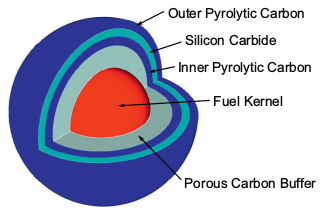
\includegraphics[height=3.5cm]{figures/triso}
	\caption{Drawing of a TRISO fuel particle. Image reproduced from \cite{hales_multidimensional_2013}.}
	\label{fig:triso}
\end{figure}

% Safety characteristics of HTGRs: Graphite and negative temp coeff
Graphite is another contributor to the passive safety of the \gls{HTGR} design.
Combining ceramic fuel and a graphite core structure permits high operating temperatures \cite{ballinger_balance_2004}.
Graphite has a high heat capacity and maintains its strength at temperatures beyond 2760 $^{\circ}$C.
Additionally, HTGRs have a negative temperature coefficient of reactivity and a low core power density.
A low core power density enables passive heat transfer mechanisms to remove the decay heat following postulated accidents \cite{neylan_modular_1988}.
These passive heat transfer mechanisms rely primarily on the natural processes of conduction, thermal radiation, and convection.
As a result, temperature changes in the core occur slowly and without damage to the core structure during transients.

% Co-generation applications: Rankine vs Bryton
HTGRs higher operating temperatures are a desirable feature because they offer increased thermal conversion efficiencies.
The early \gls{HTGR} designs converted their heat into electricity using the steam-Rankine cycle \cite{herranz_power_2009}.
In such a system, the helium coolant passes through a steam generator, and the steam drives a turbine.
This arrangement is around 38\% efficient \cite{breeze_nuclear_2014}.
However, the steam cycle requires a steam generator and also a gas circulator \cite{no_review_2007}.
This requirement increases the capital cost of power plant, and it creates a risk of a water ingress event.
The Brayton cycle is a better option because the helium coolant can directly drive a gas turbine in a closed cycle.
A closed cycle eliminates the need for a steam generator and a gas circulator.
Additionally, it removes external sources of contamination of the nuclear circuit, reducing the need for on-line cleanup systems \cite{iaea_current_2001}.
With the Brayton cycle, the system can achieve an energy conversion efficiency of around 48\% \cite{breeze_nuclear_2014}.

Higher outlet temperatures and increased thermal conversion efficiencies in HTGRs enable a wide range of process heat applications, such as coal gasification processes, oil refinery processes, and production of synthesis gas, methanol, and hydrogen.
Hydrogen offers a solution to energy and climate challenges, decarbonizing the transport and power sectors \cite{nagashima_japans_2018}.
Several hydrogen production processes benefit from high temperatures, such as high-temperature electrolysis \cite{doenitz_hydrogen_1980} or thermochemical water-splitting \cite{yildiz_efficiency_2006}.
Utilizing the \gls{HTGR} as the process energy source eliminates the need to burn fossil fuels to generate the steam those processes require \cite{iaea_current_2001}.

% Maybe this paragraph should be in objectives
This thesis focuses primarily on the \gls{MHTGR}-350 \cite{neylan_modular_1988} \cite{silady_licensing_1988}.
Under the sponsorship of the \gls{US} \gls{DOE}, a team consisting of General Atomics, Combustion Engineering, General Electric, Bechtel National, Stone \& Webster Engineering, and \gls{ORNL} developed the \gls{MHTGR}-350 \cite{neylan_modular_1988}.
They designed the basic module to deliver superheated steam at 17.3 MPa and 538 $^{\circ}$C.
Based on both economic and technological considerations, a 350 MWth modular reactor defines the optimal configuration.
The team completed in 1986 the preliminary safety information document for the MHTGR-350 and the complete draft pre-application in 1989 \cite{huning_steady_2014}.

% \cite{ballinger_balance_2004}
% The modular type HTGR provides the extra unique characteristic that the fuel temperature will not exceed the failure temperature following postulated accidents just by using passive heat transfer mechanisms.

\section{Motivation}

This work's ultimate goal is to support the development of \gls{HTGR} technology.
More specifically, we focus on the development of computational methods for modeling \glspl{HTGR} with \textit{Moltres} \cite{lindsay_introduction_2018} as our primary analysis tool.

% Why do we focus on HTGRs?
The Generation IV Roadmap project identified reactor concepts that could meet the future's energy demands in an efficient, economical, and environmentally safe manner \cite{macdonald_ngnp_2003}.
One of these reactor concepts is the \gls{VHTR}.
A \gls{VHTR} is a type of HTGR whose core outlet temperatures are between 700 and 950 $^{\circ}$C \cite{gif_gif_2019}.
The \gls{DOE} selected this reactor concept for the \gls{NGNP} Project.
This project intended to demonstrate emissions-free nuclear-assisted electricity and hydrogen production by 2015.

Although the \gls{DOE} canceled the \gls{NGNP} Project, the large scale deployment of HTGRs may become a reality in the near term.
Some microreactor designs embody this type of reactor technology and may be operational before 2030.
Additionally, as Section \ref{sec:pmr} has already described, HTGR technology has several favorable characteristics.
To recapitulate the most relevant features, the \gls{HTGR} relies on passive heat transfer mechanisms, uses TRISO particles as its fuel which inhibits proliferation, achieves high temperatures, and benefits from increased cycle efficiencies.
Another beneficial characteristic is that high temperatures enable a wide range of process heat applications, among which we find hydrogen production.

%Why is computational modeling important?
Modeling and prediction of core thermal-hydraulic behavior is necessary for assessing the safety characteristics of a reactor.
Determining the temperature inside a reactor, for both normal and transient operation, is of paramount importance as several materials' integrity depends on it.
Undesirably high temperatures endanger the TRISO particles' integrity and, consequently, jeopardize the fission product containment \cite{tak_numerical_2008}.
% The temperatures in the core have to be kept below values that begin to cause damage to fission product barriers, produce stmctural material weakness, and lead to excessive chemical reaction rates.
Furthermore, the complex fuel blocks geometry requires numerical calculations for obtaining the fuel temperatures.

The characteristics of an \gls{HTGR} are different from those of conventional \glspl{LWR}.
Such differences demand reactor analysis tools that capture the following peculiarities of \glspl{HTGR} \cite{rohde_development_2012}\cite{bostelmann_criticality_2016}:
\begin{itemize}
% \item Hexagonal structure: the shape of the fuel blocks hinders conformity to any orthogonal coordinate system.
\item Double heterogeneity: the TRISO particles form the first heterogeneity level, consisting of four
layers.
The second level arises from the fuel elements, as they encompass the compacts, the coolant, and the moderator.
\item Strong temperature dependence: the fuel temperatures have a significant effect on the neutron spectrum and the transient feedbacks.
\item High temperature gradient: the temperature difference between the fuel and the moderator is large during the course of transients.
\item High thermal inertia: the large graphite structures cause long transients.
\end{itemize}

%Why use Moltres?
Historically, linking a stand-alone neutronics solver to a thermal-hydraulics solver allowed for simulating an entire reactor.
The connection of the programs occurred in a loose-coupling fashion, such that one code's output served as the other's input and vice versa.
This coupling technique is commonly known as the operator-splitting technique \cite{ragusa_consistent_2009}.
In such an approach, each program uses a physical model that solves some of the problem variables while assuming constant the rest of them.
Nonetheless, these physical models describe processes that rely heavily on the solution of one another's.
The neutron flux determines the power distribution, and the power distribution strongly influences the temperature field.
Due to the \gls{HTGR} temperature feedback, the temperature affects the neutron flux distribution in the core.
Because of a strong temperature feedback, multiphysics transient simulations coupled via the operator-splitting approach may introduce significant numerical errors \cite{park_tightly_2010}\cite{ragusa_consistent_2009}.

\gls{MOOSE} \cite{gaston_moose_2009} is a computational framework targeted at solving fully coupled systems.
All the software built on the \gls{MOOSE} framework shares a joint code base.
These features facilitate relatively easy coupling between separate phenomena and allow for great flexibility, even with a large variance in time scales \cite{novak_pronghorn_2018}.
Additionally, all programs use \gls{MPI} for parallel communication and allow for deployment on massively-parallel cluster-computing platforms.

\textit{Moltres} is an open source, \gls{FEM} application built within the \gls{MOOSE} framework.
\textit{Moltres} solves arbitrary-group neutron diffusion, delayed neutron precursor concentration, and temperature governing equations.
All these characteristics, plus some modifications that this work intends to implement, make \textit{Moltres} suitable for solving the type of physical phenomena described above.

\section{Objectives}

% This thesis focuses on steady-state calculations and also intends to set a roadmap for the transient simulations.
As mentioned earlier, the ultimate goal of this work is to support the development of \gls{HTGR} technology.
The following list of main objectives expands on that goal.

\paragraph{Determine prismatic \glspl{HTGR} key physics.}
Prismatic HTGRs have inherent physics phenomena unique to their design.
This thesis intends to determine which are those inherent physics crucial for their accurate modeling.

\paragraph{Extend Moltres modeling capabilities to prismatic \glspl{HTGR}.}
Moltres is a multi-physics solver designed to capture key physics in \glspl{MSR}.
Moltres's current capabilities allow for solving some of the physics in the prismatic HTGR design.
Nevertheless, the solver needs to capture the missing physics in prismatic HTGRs and adequately integrate them into the current capabilities.

\paragraph{Understand \gls{HTGR} contribution to stopping climate change.}
HTGRs are an attractive technology due to attaining high temperatures.
With such high temperatures, the efficiency of hydrogen production increases.

\vskip 0.6cm
The main objectives are somewhat broad.
The following list presents secondary objectives which will lead to the fulfillment of the main objectives:

\paragraph{Demonstrate Moltres' ability to predict HTGR neutronics.}
A neutronics solver should predict the flux shape and magnitude accurately, during steady-state and transient simulations.
Previous work demonstrated Moltres' ability to solve MSR neutronics.
Chapter \ref{ch:neutronics} demonstrates such an ability for prismatic HTGRs.

\paragraph{Understand the impact of the group constants energy group structure on the HTGR diffusion calculations.}
The underlying physics of \glspl{HTGR} differ from the physics of other reactors.
Consequently, the simulation results will be sensitive to different parameters from other reactor type simulations.
Chapter \ref{ch:neutronics} studies the impact of the group constants energy group structure on the diffusion calculations.

\paragraph{Calculate power distribution correctly.}
The power distribution is the most influential parameter over the thermal-hydraulics as it determines the temperature profile in the reactor.
Previous work demonstrated Moltres ability to calculate the power distribution in MSRs.
Chapter \ref{ch:neutronics} evinces such an ability for prismatic HTGRs.

\paragraph{Predict prismatic HTGRs temperature profile accurately.}
Undesirably high temperatures endanger the integrity of the reactor structures, and most importantly, the TRISO particles.
Additionally, the temperature influences the neutronics.
Hence, an accurate neutronics calculation will be inaccurate without a correct thermal-hydraulics calculation. 
Previous work demonstrated Moltres ability to predict the temperature profile in MSRs.
Chapter \ref{ch:thermalfluids} examines Moltres ability to accurately predict the temperature profile in prismatic HTGRs.

\paragraph{Coupled simulations
Accurately model the thermal feedback on the neutronics.
Chapter \ref{ch:thermalfluids}

\paragraph{Techno-economic analysis of hydrogen production with HTGRs.}
High temperatures enable high-efficiency hydrogen production methods.
Most of them have different energy requirements and production rates.
Chapter \ref{ch:hydro} analyses such quantities.

\chapter{Literature Review}
This chapter summarizes previous efforts in numerical simulations of prismatic HTGRs.
The simulation of prismatic HTGRs require the coupled modeling of the neutronics and thermal-fluid phenomena.
This chapter comprehends the following sections: Section \ref{sec:litreview-neut} addresses diffusion methods for solving the neutronics, Section \ref{sec:litrev-thermalf} focuses on the thermal-fluids, Section \ref{sec:litreview-multi} studies the coupled simulations, and Section \ref{sec:litreview-summary} wraps up the main takeaways of the literature review.

\section{Prismatic HTGR Diffusion Solvers}
\label{sec:litreview-neut}

Currently, several software programs solve the neutronics of prismatic \glspl{HTGR}.
Most of these codes rely on one of the following methods: stochastic transport (Monte Carlo), deterministic transport, or deterministic diffusion.
This section focuses on the last class.
% If time permits work on a brief description of the Monte Carlo and deterministic transport maybe.
% Why? Deterministic diffusion solvers have lower computational requirements than other methods reference ??
% The utilization of the Monte Carlo codes is unattractive because of the tremendous problem size and the need for a large number of neutron histories \cite{lee_status_2006}.
% It is one of the simplest means to solve neutron transport problems \cite{leppanen_development_2007}.
% Here I say the following
% Deterministic diffusion methods are computationally cheaper than the other methods.
% This characteristic makes it a good candidate for coupled calculations.

The history of deterministic diffusion solvers began in the late 1950s with the \gls{FDM} application to the analysis of \glspl{LWR}.
In \gls{FDM}, mesh spacings are usually of the order of the diffusion length.
While solving large multi-dimensional problems, this feature causes the mesh points to reach intractable numbers \cite{lewis_finite_1986}.
The computational expense of these calculations motivated the generation of more computationally efficient techniques \cite{lawrence_progress_1986}.
Although substantial overlaps exist, the most common techniques fall into two broad categories: nodal methods and \gls{FEM}.

% NODAL
FLARE \cite{delp_flare_1964} is a three-dimensional \gls{BWR} simulator, and it is representative of the first generation of nodal methods.
This approach used adjusted parameters to match actual operating data or the results of more accurate calculations.
Most of these methods were implementations of the so-called "1.5 group theory" \cite{gupta_nodal_1981}.
The second generation of nodal methods derived spatial coupling relationships by applying the \gls{TIP}.
This procedure obtains equivalent one-dimensional equations by integrating the multi-dimensional diffusion equation over directions transverse to each coordinate axis \cite{lawrence_progress_1986}.
This approach proved to be highly efficient and accurate in Cartesian geometries.

In 1981, a formulation based on the \gls{NEM} first demonstrated the feasibility of nodal methods in hexagonal geometries \cite{duracz_nodal_1981}.
However, this method would introduce non-physical singular terms that required the utilization of discontinuous polynomials.
This drawback motivated the development of more effective formulations.
HEXNOD, introduced in 1988 by Wagner \cite{wagner_three-dimensional_1989}, is an example of such formulations.
This algorithm uses the \gls{TIP} and, in contrast to the \gls{NEM}, solves the resulting differential equation analytically.
Wagner's article demonstrated the method's good accuracy by comparing to \gls{FDM} and Monte Carlo calculations for a few benchmark problems.

HEXPEDITE \cite{fitzpatrick_hexpedite_1992} introduced a new method that is another example of more effective formulations.
HEXPEDITE uses the \gls{TIP} formulation to derive a pseudo-one-dimensional equation.
The resulting differential equation is solved analytically.
The difference from HEXNOD is that HEXPEDITE uses a simpler and more efficient coupling scheme.
Different works \cite{fitzpatrick_hexpedite_1992}\cite{fitzpatrick_developments_1995} on the HEXPEDITE methodology tested the approach against the \gls{NEM} and the \gls{FDM}.
These studies established HEXPEDITE’s superiority in terms of accuracy and runtime.
HEXPEDITE's use prevailed in the analysis of \glspl{HTGR} until recently.
In 2010, \gls{INL} conducted a study \cite{ortensi_deterministic_2010-1} in which they compared HEXPEDITE's results against several diffusion codes, as well as the Monte Carlo codes MCNP5 \cite{rsicc_computer_code_collection_mcnp5_2003} and Serpent \cite{leppanen_serpent_2015}.
% In 2010, \gls{INL} conducted a study \cite{ortensi_deterministic_2010-1} in which they compared HEXPEDITE's results against the diffusion codes JAR, CITATION, and CRONOS2, as well as the Monte Carlo codes MCNP5 and Serpent.

DIF3D \cite{lawrence_dif3d_1983} and PARCS \cite{downar_parcs_2004} are other examples of prevalent nodal diffusion codes.
DIF3D has several solution options such as the diffusion \gls{FDM}, diffusion \gls{NEM} based on \gls{TIP}, and the VARIANT nodal transport method.
% VARIANT: variational nodal \cite{palmiotti_variant_1995}
PARCS has several solution options as well, such as a diffusion \gls{FDM}, diffusion \gls{NEM} based on \gls{TIP}, P$_{N}$ transport methods, and the multigroup transport simplified P$_3$ with \gls{FDM} and \gls{NEM} discretizations.

% from ortensi_deterministic_2010-1 and wang_modified_2018
Nodal methods solve relatively coarse meshes for approximate solutions.
This characteristic makes the process efficient.
On the other hand, the method does not provide detailed point-wise accurate solutions \cite{kang_finite_1973}.
Additionally, the derivation of nodal methods happens in a specific coordinate system for a particular node shape.
The application to complex problems is not flexible as different geometries require customized configurations.
This lack of flexibility limits the applications of nodal methods to regular geometries only.

% FEM
The \gls{FEM} is a well-established method in applied mathematics and engineering.
\gls{FEM} is a numerical technique for finding approximate solutions to partial differential equations by deriving their weak or variational form.
Most applications make \gls{FEM} preferable due to its flexibility in the treatment of curved or irregular geometries.
Also, the use of high order elements attains higher rates of convergence \cite{cavdar_finite_2004}.
The first engineering application of \gls{FEM} was in the field of structural engineering dating back to 1956.
In successive years, \gls{FEM} became the most extensively used technique in almost every branch of engineering.
\glspl{FEM} have several advantages over the nodal methods.
It provides flexibility in the geometry definition, a firm mathematical basis, ease in extension to the multi-group application, and high computational efficiency \cite{lee_development_2008}.

In 1973, Kang et al. \cite{kang_finite_1973} described the first application of \gls{FEM} to neutron diffusion theory.
The fundamental motivation for this development was the impractical application of the \gls{FDM} to three-dimensional problems.
In this early work, the author compared different \gls{FEM} approaches to the \gls{FDM} in one-dimensional and two-dimensional problems.
The studies showed a higher order of convergence achieved by the \gls{FEM}.

Throughout the last four decades, many software programs utilized the \gls{FEM} to solve the diffusion equation.
Some of the most recent software for diffusion simulations are CRONOS2 \cite{lautard_cronos_1990}, CAPP \cite{lee_development_2011}, and Rattlesnake \cite{wang_rattlesnake_2019}.
The list of \gls{FEM} diffusion solvers is more extensive, but we focus on the best-documented software in the open literature.
% We also emphasize that most of the \gls{FEM} diffusion solvers for \glspl{HTGR} were born as \gls{LWR} analysis codes.

% CRONOS
\gls{CEA} developed CRONOS2 \cite{lautard_cronos_1990} as part of the SAPHYR system.
CRONOS2 conducts steady-state and transient multi-group calculations, based on the diffusion equation or the transport equation using the S$_N$ method and an \gls{FDM} or a \gls{FEM} discretization.
In 2008, Damian et al. \cite{damian_vhtr_2008} presented the code suite NEPTHIS\cite{cavalier_presentation_2005}/CAST3M\cite{studer_cast3marcturus_2007}, software that relied on CRONOS2.
Section \ref{sec:litreview-multi} describes further the coupling scheme.

% CAPP
In 2008, the \gls{KAERI} published an article \cite{lee_development_2008} that presented CAPP.
Its purposes are to conduct steady-state core physics analysis, core depletion analysis, and core transient analysis.
The article validated the software with two benchmark problems: the IAEA PWR benchmark problem, and Phase I Exercise 1 of the OECD/NEA PBMR-400 Benchmark \cite{reitsma_oecd-neansc_2008}.
In 2011, Lee et al. published an article \cite{lee_development_2011} in which they extended the functionalities of CAPP to prismatic HTGRs.
To validate CAPP, they had to add to CAPP a simplified thermal-fluids tool.
Section \ref{sec:litreview-multi} describes the thermal-fluids tool and their coupling.

% Proghorn and Rattlesnake
RattleSnake \cite{wang_rattlesnake_2019} is the MOOSE \cite{gaston_moose_2009} based application for simulating the transport equation.
\gls{INL} had initially developed Pronghorn \cite{novak_pronghorn_2018} to model \glspl{PBMR} \cite{strydom_inl_2013}.
The MOOSE neutronics kernel library Yak incorporated the neutron diffusion models initially in Pronghorn.
Currently, RattleSnake is the primary tool for solving the linearized Boltzmann neutron transport equation within MOOSE and relies heavily on Yak.
Various solvers are available under RattleSnake, including low-order multigroup diffusion, spherical harmonics transport, and discrete ordinates transport, all solved with the \gls{FEM}.
% Both RattleSnake and Pronghorn yielded the same exact results when using the continuous \gls{FEM} multigroup diffusion option in RattleSnake.

% strydom_inl_2013
In 2013, \gls{INL} conducted the OECD/NEA MHTGR-350 MW Benchmark \cite{oecd_nea_benchmark_2017}\cite{strydom_inl_2013} without further simplifications.
The \gls{INL} team solved Phase I Exercise 1 using INSTANT-P1 \cite{wang_krylov_2011}, Pronghorn, and RattleSnake.
% They also solved exercises 2 and 3 using RELAP5-3D and PHISICS/RELAP5-3D code suit.
INSTANT-P1 is a transport solver that relies on the spherical harmonics discretization of angles.
The results for Pronghorn and RattleSnake were identical.
By modifying the cross-sections, INSTANT-P1 returned the diffusion solution.
Its results were within 30 pcm from Pronghorn and RattleSnake results.
All presented results exhibited good agreement with the benchmark results.

\subsection{Energy group structure analysis}
\label{sec:energy-struct}

% Number of energy groups impact over the calculations
Diffusion calculations use homogenized group constants previously generated by neutron transport solvers.
The choice of the energy group structure for the group constant homogenization affects the accuracy of the diffusion calculation.
The longer neutron mean free path in \glspl{HTGR} compared to \gls{LWR} increases the spectral interactions between elements.
For this reason, HTGR analyses require more energy groups than conventional \gls{LWR} analyses.
This section summarizes previous studies on the impact of the energy group structure over the diffusion calculations.

\gls{ANL} directed a study \cite{lee_status_2006} to compare the accuracy of nodal diffusion calculations employing different energy group structures.
The group constant homogenization used the DRAGON neutron transport solver and the diffusion calculations utilized the code DIF3D.
For the study, the ANL team implemented a one-dimensional fuel-reflector model in which they compared the solution accuracy using 4, 7, 8, 14, and 23 energy groups.
They also used alternative energy group structures for the same number of groups.
For simplicity, the authors used the homogenized fuel compact model and generated all the group constant at 300 K.
One of their conclusions was that the number of energy groups should be more than 4, and more than 6 would be sufficient for uranium fueled HTGRs.
Another finding was that the accuracy of the diffusion calculation is sensitive to the energy group boundaries.
% Mention something about the metrics of the study? To asses the accuracy, they compared the multiplication factor.

% \begin{figure}[htbp!]
% 	\centering
% 	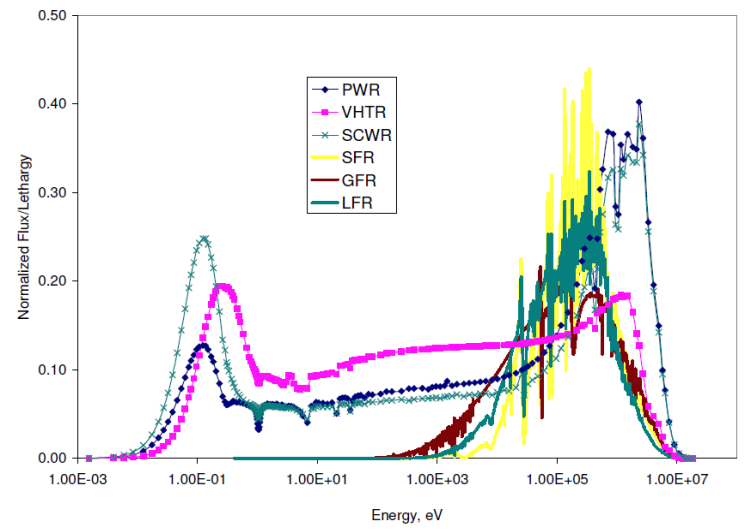
\includegraphics[width=0.40\linewidth]{figures/spectrum}
% 	\caption{Comparison of neutron energy spectra of different reactor designs. PWR=Pressurized Water Reactor, VHTR=Very High-Temperature Gas-Cooled Reactor, SCWR=Supercritical Water Reactor, SFR=Sodium Fast Reactor, GFR=Gas Fast Reactor, LFR=Lead Fast Reactor. Image reproduced from \cite{taiwo_summary_2005}.}
% 	\label{fig:spectrum}
% \end{figure}

% han_sensitivity_2008
Han's MS thesis \cite{han_sensitivity_2008} focused on selecting energy groups for the reactor analysis of the \gls{PBMR}.
The author used COMBINE6 \cite{grimesey_combinepc-portable_1994} for group constant generation and the Penn State nodal diffusion code NEM \cite{bandini_three-dimensional_1990} for the reactor analysis.
The author compared the results against MCNP5 reference results.
To simplify the setup, the model used uniformly distributed isotopes in the fuel.
The study performed the calculations at 300 and 1000 K.
To arrive at an optimal group structure, the author compared many combinations of group structures using a trial and error strategy.
One conclusion of this work agrees with the previous bibliography \cite{gulf_oil_company_nuclear_1973} \cite{duderstadt_nuclear_1976} in that the energy spectrum is critical to yield an accurate description of a nuclear reactor using a few groups.

ANL's study helps set up proper nodal diffusion calculations for an \gls{HTGR}.
Although we can extrapolate those conclusions to \gls{FEM} diffusion solvers, such a study might be valuable as a part of this thesis.
ANL's team conducted the study at 300 K --- not in the operational range of any \glspl{HTGR}.
On the contrary, Han's thesis included an analysis at 1000 K, and his results showed that the temperature changes have a non-negligible impact.
Additionally, ANL's study used the simplified model of the homogenized fuel compact.
Han highlighted that homogenized fuel models of the \gls{PBMR} underestimate criticality calculations.
In 2015, \gls{INL} presented their results \cite{strydom_results_2015} for an \gls{IAEA} coordinated research project \cite{tyobeka_htgr_2011} and showed that the homogenization of the compact material notably underestimates the multiplication factor.
On the other hand, the open literature has not investigated the impact of such simplification over the homogenized group constants.

\subsection{Summary of Prismatic HTGR Diffusion Solvers}

Section \ref{sec:litreview-neut} introduced several deterministic diffusion classes, including FDM, nodal methods, and FEM.
The fundamental motivation for the development of nodal methods and FEM was the impractical application of the \gls{FDM} to three-dimensional problems.
Section \ref{sec:litreview-neut} also discussed on the main characteristics of these methods, directing the reader's attention to the advantages of the FEM.
Although nodal methods are efficient, most applications make FEMs preferable due to its flexibility in the treatment of irregular geometries.
Additionally, FEMs have a firm mathematical basis, and its formulation eases the extension to multi-group applications.
Moltres relies on the FEM counting with all the advantages of the method.

Section \ref{sec:litreview-neut} summarizes previous efforts in deterministic diffusion solvers of prismatic HTGRs.
This thesis draws two main conclusions from those earlier efforts.
The first conclusion is that several authors validated their solvers by comparison to other codes.
In the context of this thesis, Chapter \ref{ch:neutronics} compares Moltres results to Serpent and the Phase I Exercise 1 of the OECD/NEA MHTGR-350 MW Benchmark.
The second conclusion is that several prismatic HTGRs count with integrated thermal-fluids solver.
Due to a strong thermal feedback, modeling of prismatic HTGRs with Moltres will require the incorporation of a thermal-fluids solver.
Section \ref{sec:litrev-thermalf} discusses previous work in the thermal-fluids modeling of prismatic HTGRs.

% energy group study
Section \ref{sec:energy-struct} outlines the importance of the right choice of energy group structure for group constant homogenization.
Diffusion calculations use homogenized group constants previously generated by neutron transport solvers.
Previous studies focused on nodal diffusion calculations of HTGRs.
Although we can extrapolate the conclusions of those conclusions to \gls{FEM} diffusion calculations, such a study might be valuable.
Chapter \ref{ch:neutronics} studies the accuracy of the diffusion calculations for different energy group structures.

\section{Prismatic HTGR Thermal-fluids}
\label{sec:litrev-thermalf}

% sort of motivation
This section of the literature review summarizes previous work on thermal-fluids modeling of prismatic HTGRs.
Thermal-fluids calculations enable the correct design of \glspl{HTGR}.
Predicting the maximum fuel temperature at steady-state is of paramount importance to succeed in such a task.
I emphasize this statement in the case that hydrogen production is desirable, as that process requires higher coolant temperatures, leading to high fuel and reactor vessel temperatures.
This literature review analyzed several approaches that helped choosing a thermal-fluids model to implement in Moltres simulations.

% sort of intro to simplified models
The complex geometry of the hexagonal fuel assembly requires numerical calculations for obtaining accurate evaluations.
Thermal-fluids studies for early \glspl{HTGR} consisted mainly of support calculations for \gls{NRC} safety analysis reports.
The analyses employed sets of independent solvers that relied on simplified approximations.
Simplified models help understand some fundamental aspects of prismatic HTGRs and have the advantage of reducing the computational expense of the calculations.

% shenoy_htgr_1974
General Atomics \cite{shenoy_htgr_1974} developed the first set of software libraries that relied on simplified approximations.
The following list introduces and summarizes some of these and their features:

\begin{itemize}
\item FLAC: It determines the coolant flow distribution in the coolant channels and gaps.
It solves the one-dimensional momentum equation for incompressible flow and the continuity equations for mass and energy.

\item POKE: It determines the coolant mass flow, coolant temperature, and fuel temperature distribution.
It solves the steady-state mass and momentum conservation equations for parallel channels.

\item DEMISE: It determines the steady-state three-dimensional temperature distribution in a standard element.
It solves the temperature in a network model.

\item TAC2D: It is a general-purpose thermal analysis code.
It solves the two-dimensional heat conduction equation.
\end{itemize}

Several studies have used these software programs.
% macdonald_ngnp_2003
For example, \gls{INL} conducted in 2003 a design study \cite{macdonald_ngnp_2003} in support of the \gls{NGNP} project.
It investigated ways to increase the coolant temperature for the NGNP.
The authors conducted several parametric studies whose reference reactor was the GT-MHR \cite{general_atomics_gas_1996}.
Using POKE and TAC2D, they evaluated three major design modifications: reducing the bypass flow, controlling the inlet coolant flow distribution, and increasing the height of the reactor.

Among the simplified approaches, this thesis differentiates the \textit{flow network}, \textit{equivalent cylindrical}, and \textit{unit cell} models.
The flow network model treats the coolant flow paths in the core as a cross-connected flow network \cite{shenoy_htgr_1974}.
Constant pressure nodes connected to flow branches make up the network.
The model uses the one-dimensional conservation momentum equations to solve the pressure loss and coolant temperature in each network node.
The equivalent cylinder model uses a geometrically simpler one-dimensional or two-dimensional design model \cite{shenoy_htgr_1974}\cite{tak_numerical_2008}.
The unit cell model divides the fuel blocks into triangular-shaped unit cells.
The model assumes that the unit cell is a symmetry section such that the coolant removes all the heat generated in the cell \cite{tak_numerical_2008}.

% flow network model
% reza_design_2006
Using the flow network analysis tool RELAP5-3D/ATHENA \cite{inl_relap5-3dathena_2005}, Reza et al. \cite{reza_design_2006} conducted a thermal-fluids study of the GT-MHR.
Reza et al. increased the reactor outlet temperature to enable hydrogen production.
Additionally, they evaluated alternative inlet coolant flow configurations in an attempt to reduce the reactor vessel temperatures.
After finding an optimal configuration, they evaluated the fuel and the reactor vessel's maximum temperatures during the \gls{LPCC} and the \gls{HPCC} events.

% equivalent cylindrical model
% no_multi-component_2007
An example of an application using the equivalent cylindrical approach is GAMMA \cite{lim_gamma_2006}\cite{no_multi-component_2007}.
GAMMA is a system code for thermal-fluids analysis and system transients.
GAMMA's primary motivation is simulating the air ingress event following a LOCA.
Following the depressurization of helium in the core, air could potentially enter the core through the break and oxidize the in-core graphite structure.
Graphite oxidation is an exothermic chemical reaction and, thus, it is a significant concern.
GAMMA solves heat conduction, fluid flow, chemical reactions, and multi-component molecular diffusion.
The code couples the solid and gas equations using the porous media model.
Together with the multi-dimensional analysis feature, GAMMA has a one-dimensional analysis capability for  modeling a flow network.

% takada_core_2004
Takada et al. \cite{takada_core_2004} carried out another study using the flow network and the equivalent cylindrical model.
Focusing on the \gls{HTTR}, they developed a thermal-fluids design tool.
This tool used the flow network analysis software FLOWNET \cite{maruyama_verification_1988} for calculating the coolant flow and temperature distributions.
TEMDIM \cite{maruyama_verification_1988} solved the fuel temperatures using the equivalent cylindrical model.
Finally, the authors validated the calculation scheme by comparing its results with the experimental data from the \gls{HTTR}.

% unit cell model
% nakano_conceptual_2008
Nakano et al. \cite{nakano_conceptual_2008} studied different fuel assembly configurations using several simplified approximations.
The authors used FLOWNET and TAC2D for determining the flow distribution and fuel temperature.
The fuel temperature calculation used the equivalent cylindrical model of a unit cell.
However, the asymmetry of the unit cell configuration makes the temperature distribution asymmetric in the graphite block, behavior that the equivalent cylindrical model fails to capture.

% in_three-dimensional_2006
In 2006, In et al. \cite{in_three-dimensional_2006} conducted a more detailed analysis using a three-dimensional model of the unit cell in the hot-spot of the GT-MHR 600, which is the spot in the core with the largest power density.
The objective of the study was to predict the maximum fuel temperature at steady-state at the end of the equilibrium cycle.
The \gls{CFD} software CFX 10 \cite{ansys_inc_cfx_2006} calculated the three-dimensional temperature profile.
The results showed that the maximum fuel temperature surpassed the design limits, so the authors proposed decreasing the power density or the axial power peak as countermeasures.

% more detailed calculations
To recapitulate, previous work used simplified approaches to evaluate different aspects of prismatic HTGRs.
Some of those evaluations include thermal-fluids design, analaysis of alternative coolant flow configurations, and accident analysis.
Such simplified approaches are helpful to understand essential aspects of prismatic HTGRs but they may yield inaccurate temperature distributions \cite{tak_numerical_2008}.
More detailed thermal-fluids evaluations were rare in the open literature until the last 15 years.
This thesis summarizes some of those evaluations down below.

% cioni_3d_2005
Cioni et al. \cite{cioni_3d_2005} presented an article in 2005 in which they conducted three-dimensional simulations of HTGR fuel assemblies.
The study's objective was to investigate the blockage of cooling channels in the core.
They used the \gls{CFD} tool Trio\_U \cite{bieder_priceles_2000} to carry out the analysis.
The numerical scheme solved the three-dimensional conduction equation in the solid coupled to the coolant's one-dimensional thermal-fluid equations.
The blockage increased the temperature on the blocked fuel assembly only and it did not affect the surrounding elements due to the bypass flow.
This study proves the importance of the bypass flow modeling.

% simoneau_three-dimensional_2007
Simoneau et al. \cite{simoneau_three-dimensional_2007} analyzed the transient behavior of an \gls{HTGR} during the \gls{DCC} and \gls{HPCC} event.
The CFD tool STAR-CD \cite{computational_dynamics_limited_star-cd_2004} performed the calculations.
It solved conductive, convective, and radiation heat transfer in a 30$^{\circ}$-section of the core and reactor vessel.
The tool used the porous media model to accommodate the different spatial scales.

% tak_numerical_2008
In 2008, an article by Tak et al. \cite{tak_numerical_2008} conducted a three-dimensional CFD analysis of a fuel column of the PMR600, a pre-conceptual reactor designed by \gls{KAERI} whose reference design is the GT-MHR.
The commercial software CFX 11 \cite{ansys_incorporated_cfx_2006} performed the calculations.
The study considered a $1/12^{th}$ section of the fuel due to its symmetry.
Using the one-dimensional thermal-fluid equations, the model determined the coolant distribution, which served as input to the CFD code.
However, the friction in the channels is dependent on the viscosity, which is highly dependent on the temperature.
Therefore, obtaining the mass flow rates from a separate solver may introduce errors \cite{sato_computational_2010}.

% sato_computational_2010
Another article \cite{sato_computational_2010} studied a $1/12^{th}$ section of the fuel column of the GT-MHR with the commercial tool FLUENT \cite{fluent_inc_fluent_2006}.
The authors conducted parametric studies of several factors, such as bypass gap-width, turbulence model, axial heat generation profile, and geometry changes due to irradiation.
In this study, FLUENT obtained the coolant distribution as part of the solution.
Their most relevant results show that the bypass flow causes a large lateral temperature gradient in the block.
Large temperature gradients cause excessive thermal stresses, which raise potential structural issues.

% travis_thermalhydraulics_2013
Despite the recent developments in CFD tools, a detailed full-core analysis for a prismatic \gls{HTGR} still requires a tremendous computational expense.
This requirement is mostly due to the three-dimensional CFD simulation of the coolant flow.
Travis et al. \cite{travis_thermalhydraulics_2013} developed a method to compute full-core thermal-fluids analyses of HTGRs.
The article presented a simplified method that reduces the computational time and memory requirements while maintaining accurate results.
The method solves the three-dimensional heat conduction equation in the solid and the one-dimensional thermal-fluid equations in the coolant channels.
The method's validation analyzed a fuel column and compared the results to those of a three-dimensional CFD simulation.
The CFD simulation used the commercial software STAR-CCM+ \cite{cd-adapco_star-ccm_2012}.
The new computational scheme reduced the computation time to 2.5\% of the CFD simulation time.
Overall, the method showed good accuracy and less than a 2\% difference to the CFD simulation.

% tak_practical_2012 / tak_development_2014
Tak et al. \cite{tak_practical_2012} \cite{tak_development_2014} developed CORONA, which uses a practical method for the whole core analysis.
CORONA intends to combine the accuracy from CFD tools and the light computational expense of system analysis codes.
The method solves the three-dimensional heat conduction equation in the solid and the one-dimensional thermal-fluid equations in the fluid.
To validate CORONA, the authors analyzed a fuel column and compared their results against CFX and experimental results.
The validation results showed that CORONA provided reasonably accurate results.

\subsection{Summary of Prismatic HTGR Thermal-fluids}

Section \ref{sec:litrev-thermalf} summarizes previous work on the thermal-fluids modeling of prismatic HTGRs.
Although CFD techniques compute detailed temperature profiles, their fine mesh requirement restricts the use of such methods to studies of the local behavior of a fuel column.
However, a whole-core thermal analysis has many advantages over local models.
In general, the problem set up includes more accurate boundary conditions.
Without whole-core modeling, the local models' mass flow distributions are average values of the core flow rate instead of their exact value \cite{huning_novel_2016}.
This simplification leads to under-predicted fuel temperatures for the assemblies with a lower flow rate than the average.
Additionally, a coupled analysis with a reactor physics code requires a full-core model \cite{tak_practical_2012}.
An alternative for an explicit whole-core analysis are system codes that use simplified models.
Nevertheless, the simplification of the geometries reduces the fuel block temperature resolution.

% porous media
% disadvantages ?

The high computational expense of CFD analysis is mostly due to the three-dimensional CFD simulation of the coolant flow \cite{travis_thermalhydraulics_2013}.
Another alternative is to combine the three-dimensional heat conduction equation for the solid structures to the one-dimensional fluid conservation equations.
The one-dimensional fluid approximation does not resolve the boundary layer avoiding finer meshes near the walls as well as turbulence conservation equations \cite{tak_development_2014}.
Chapter \ref{ch:thermalfluids} studies the implementation of this alternative in Moltres for studying the thermal-fluids of prismatic HTGRs.

\section{Prismatic HTGR Multi-physics}
\label{sec:litreview-multi}

% sort of intro
Historically, stand-alone simulations have solved the neutronics and thermal-fluids of HTGRs separately.
Nonetheless, these physical phenomena rely heavily on one another.
Hence, a coupled analysis is necessary to consider the interaction between the neutronics and thermal-fluids behavior \cite{tak_cappgamma_2016}.

% damian_vhtr_2008
In 2008, Damian et al. \cite{damian_vhtr_2008} conducted a study aimed at understanding the passive safety features of a prismatic \gls{HTGR}.
They performed analyses on various geometrical scales, including: unit cell and fuel columns located at the core hot-spot and two-dimensional and three-dimensional core configurations, including the coupling between neutronics and thermal-fluids.
The last part of the study analyzed a three-dimensional core model using the coupled software NEPTHIS and CAST3M/Arcturus for calculating the neutronics and the thermal-fluids.
NEPHTIS used a transport-diffusion calculation scheme that relied on APOLLO2 \cite{sanchez_apollo2_1999} and the diffusion code CRONOS2.
The CAST3M/Arcturus model used a two-level approach.
On the first level, the porous media model solved the homogenized system and the coolant.
On the second level, CAST3M solved the thermal-fluids on the homogenized geometry.
The authors conducted several parametric studies and assessed their impact on the power distribution.
The studies included the variation of the helium bypass fraction, average power density, core geometry, reflector materials, and fuel loading strategy.
Their results exhibited that with the reduction of the bypass fraction, the average reflector temperature rises.

% CAPP
In 2011, Lee et al. published an article \cite{lee_development_2011} in which they extended the functionalities of CAPP to prismatic \glspl{HTGR}.
To take into account the thermal feedback, the authors integrated into CAPP a simplified thermal-fluids tool based on Stainsby's approach \cite{stainsby_investigation_2008}.
This approach uses different lenght scale models to solve the temperature distribution.
The model divides a fuel column into six triangular prisms, each of them hosting a representative coolant channel.
The tool calculates the axial coolant temperature distribution solving the energy equation.
After calculating the coolant temperature, a two-dimensional conduction model solves the moderator and fuel compact temperatures.
Through a TRISO particle conduction model, the model obtains the fuel temperature.
Finally, a three-dimensional conduction model based on the \gls{FDM} allows for solving the reflector temperature.
To validate this model, the authors solved a two-dimensional model of the PMR-200 at the beginning of the equilibrium cycle.
The PMR-200 is a pre-conceptual reactor designed by \gls{KAERI}.
Their validation compared the results against HELIOS \cite{stammler_helios_1998}, concluding with a strong accuracy.

% tak_cappgamma_2016
Tak et al. \cite{tak_cappgamma_2016} coupled CAPP and GAMMA+.
GAMMA uses the one-dimensional form of the mass, momentum, energy, and species conservation equations to solve the fluid's flow and temperature distribution.
For solids, it uses three different models: (1) heat conduction model of a TRISO particle, (2) implicit coupling to consider the heat exchange between a fuel compact and TRISO particle, and (3) multi-dimensional heat conduction model of the hexagonal fuel and reflector blocks.
In this study, the authors applied the coupled code to study the steady-state performance of the PMR-200.
Some of their most relevant results revealed that neglecting the bypass flow decreases the active core temperatures; consequently, the multiplication factor increases by approximately 300 pcm.
These results prove the importance of the right modeling of the thermal-fluids in coupled simulations of prismatic HTGRs.

% yuk_time-dependent_2020
A recent article by Yuk et al. \cite{yuk_time-dependent_2020} added to CAPP the capability to conduct transient analyses.
This capability solves the time-dependent neutron diffusion equation with the \gls{FEM}.
The primary motivation behind this feature was to perform reactivity insertion accident simulations.
To take into account the thermal feedback, the authors developed a simplified thermal-fluids analysis tool based on Stainsby's approach.
The tool divides a fuel column into six triangular prisms, each of them hosting a representative coolant channel.
After calculating the coolant temperature, a two-dimensional conduction model solves the moderator and fuel compact temperatures.
To test the new transient capabilities, they analyzed two control rod ejection scenarios and compared the results to those of the CAPP/GAMMA+ coupled code.
Both showed similar results.
This article highlights the importance of developing transient analysis capabilities to conduct accident simulations.

% Benchmarks Intro
The prismatic HTGR tools available have lagged behind tools and methods developed for \glspl{LWR}.
The evolution of the HTGR technology drives the development of more accurate and efficient simulation tools.
Additionally, the definition appropriate benchmarks is essential to compare various tools' capabilities.
% oecd_nea_coupled_2020
In 2012, the \gls{OECD}/\gls{NEA} defined a benchmark for the \gls{MHTGR}-350 MW reactor \cite{oecd_nea_benchmark_2017}.
The purpose of this benchmarking exercise is to compare various reactor physics and thermal-fluid analysis methods.
The MHTGR-350 design serves as a basis for this benchmark.
The scope of the benchmark is twofold: (1) to establish a well-defined problem, based on a common given data set, to compare methods and tools in core simulation and thermal-fluid analysis, and (2) to test the depletion capabilities of various lattice physics tools available for prismatic \glspl{HTGR}.
The OECD/NEA MHTGR-350 MW benchmark subdivides the coupled system calculation into three phases.
Phase I corresponds to the steady-state modeling of the stand-alone neutronics and thermal-fluids, as well as the coupling between them.
Phase II consists of transient cases.
Phase III focuses on lattice depletion calculations.

% j_ortensi_relap-7_2012 j_ortensi_initial_2012
In 2012, \gls{INL} published a study \cite{j_ortensi_initial_2012} that coupled Pronghorn and RELAP-7 \cite{andrs_relap-7_2012}.
Pronghorn solved the coupled equations defining the neutron diffusion, fluid flow, and heat transfer in a three-dimensional model.
RELAP-7 is a MOOSE-based system application and solves the one-dimensional continuity, momentum, and energy equations for a compressible fluid.
It was responsible for simulating the plant system layout, including the hot and cold ducts, the helium circulator, and the steam generator.
% This study integrated PRONGHORN and RELAP-7 with the operator split approach (or loose coupling) where each application used an independent mesh.
To test the coupling, INL's team carried out the OECD/NEA MHTGR-350 Benchmark \cite{oecd_nea_coupled_2020}.
The original benchmark provides a set of 26 neutron energy group and temperature dependent cross sections.
To simplify the debugging, the authors collapsed the 26 groups into two groups.
Although using two groups reduces the accuracy of the model, the lower number of groups decreases the calculation time by at least a factor of ten.
In this study, a two-dimensional cylindrical model replaced the three-dimensional geometry defined by the benchmark.
The integrated system testing included two stages: (1) both stand-alone codes underwent several convergence studies, and (2) the integrated system solved the steady-state problem in an integrated manner.
The authors concluded that the coupling between Pronghorn and RELAP-7 was successful.

% tak_coupled_2016
Tak et al. \cite{tak_coupled_2016} developed a neutronics/thermal-fluids coupled software using DeCART \cite{kaeri_decart_2007} and CORONA.
DeCART is a whole-core neutron transport tool, and it was responsible for calculating the power distribution and the fast neutron fluence.
CORONA calculated the temperature distribution.
To validate the code, the authors conducted the OECD/NEA MHTGR-350 benchmark.
The exercise's main objective was to validate the code and identify technical challenges for future development.
The authors presented an interesting analysis in which they compared the coupled simulation results and the stand-alone simulations.
The difference in the multiplication factor was as high as 2597 pcm.
The axial offset and maximum fuel temperature exhibited significant differences as well.
This study highlights the importance of the integration of both neutronics and thermal-fluid solvers.

% tyobeka_htgr_2011 / strydom_results_2015
Sensitivity analysis and uncertainty analysis methods assess the predictive capabilities of coupled neutronics/thermal-fluids simulations.
In 2013, the IAEA launched a coordinated research project \cite{tyobeka_htgr_2011} on the HTGR Uncertainty Analysis in Modeling.
The coordinated research project's objective was to determine the uncertainty in HTGR calculations at all stages of coupled reactor physics/thermal-fluids and depletion calculations.
This coordinated research project is a natural continuation of the previous IAEA and OECD/NEA international activities \cite{iaea_evaluation_2003}\cite{reitsma_oecd-neansc_2008} on Verification and Validation of available HTGR simulator capabilities.
The technical approach is to establish and utilize a benchmark for uncertainty analysis.
The benchmark defines a series of well-defined problems with complete sets of input specifications and reference experimental data.
The coordinated research project adopted the MHTGR-350 as the reference design and the GT-MHR as a second reference design.
The design specification uses the OECD/NEA MHTGR-350 MW benchmark \cite{oecd_nea_benchmark_2017} code design specifications.
The coordinated research project subdivides the coupled system calculation into three phases.
Phase I corresponds to the stand-alone neutronics and thermal-fluids modeling.
Phase II consists of design calculations, coupled with steady-state neutronics/thermal-fluids calculations with and without depletion calculations.
Phase III focuses on safety calculations.

\subsection{Summary of Prismatic HTGR Multi-physics}

Section \ref{sec:litreview-multi} introduced several prior studies of prismatic HTGR multi-physics.
This studies highlight the importance of the proper integration of the neutronics and thermal-fluids in HTGR modeling.
The neutronics and thermal-fluids physical phenomena rely heavily on each other.
Hence, a coupled analysis is necessary to capture the interaction between the neutronics and the thermal-fluids.
Chapter \ref{ch:thermalfluids} discusses a coupling strategy for the neutronics and thermal-fluids phenomena in Moltres.
For that exercise, Section \ref{sec:coupled-average} follows a simplified version of Phase I Exercise 3 of the OECD/NEA MHTGR-350 MW Benchmark.


\chapter{Methodology}

\section{Computational tools}

\subsection{MOOSE}

% intro
\gls{MOOSE}\cite{gaston_moose_2009} is a computational framework that supports engineering analysis applications.
In a nuclear reactor, several partial differential equations describe the physical behavior.
These equations are typically nonlinear, and they are often strongly coupled to each other.
\gls{MOOSE} targets such systems and solves them in a fully coupled manner.

% more details about MOOSE
\gls{MOOSE} is an open-source code under a \gls{LGPL}.
The code itself relies on LibMesh \cite{kirk_libmesh_2006}, an LGPL finite element library, and PetSc, a \gls{BSD}-licensed toolkit for solving nonlinear equations \cite{balay_petsc_2016}.
MOOSE applications define weak forms of the governing equations and 
modularize the physics expressions into "Kernels."
Kernels are C++ classes containing methods for computing the residual and Jacobian contributions of individual pieces of the governing equations.
\gls{MOOSE} and LibMesh translate them into residual and Jacobian functions.
These functions become inputs into PetSc solution routines.

\gls{MOOSE} utilizes the mathematical structure present in \gls{JFNK} methods \cite{knoll_jacobian-free_2004}.
\gls{JFNK} methods are synergistic combinations of Newton-type methods for superlinearly convergence of nonlinear equations and Krylov subspace methods for solving the Newton correction equations.
The Jacobian-vector product links the two methods.
JFNK methods compute such products approximately without forming and storing the elements of the true Jacobian.
The ability to perform a Newton iteration without forming the Jacobian gives JFNK methods potential for application throughout problems governed by nonlinear partial differential equations.

All the software built on the MOOSE framework shares a joint base code.
The applications, by default, utilize monolithic and implicit methods.
This feature facilitates relatively easy coupling between different phenomena and allows for great flexibility, even with a great variance in time scales \cite{novak_pronghorn_2018}.
Additionally, all codes use \gls{MPI} for parallel communication and allow deployment on massively-parallel cluster-computing platforms.

\subsection{Moltres}

\textit{Moltres} \cite{lindsay_introduction_2018} is a MOOSE-based application initially designed for modeling fluid-fuelled \glspl{MSR}.
This simulation tool is open source and operates with an LGPL.
It uses \textit{git} for version control, emphasizing its openness and promoting quality through peer review.

Moltres solves arbitrary-group neutron diffusion, precursors, and temperature governing equations.
It can solve the equations in a fully-coupled way or solve each system independently, allowing for great flexibility and making it applicable to a wide range of nuclear engineering problems.

\subsection{Serpent}

The Serpent Monte Carlo code \cite{leppanen_development_2007} \cite{leppanen_calculation_2014} is a three-dimensional continuous-energy neutron transport code developed by the VTT Technical Research Centre of Finland, and it has been in public distribution since 2009.
Monte Carlo neutron transport codes have several reactor physics applications related to criticality safety analyses, radiation shielding problems, detector modeling, and validation of deterministic transport codes.
The Monte Carlo method's main advantage is its capability to model geometry and interaction physics without significant approximations.
The main disadvantage is that simulating complex systems is computing-intensive, restricting applications to some extent.

Serpent serves two primary purposes: (1) reactor modeling, and (2) group constant generation.
In reactor modeling, the Monte Carlo simulation itself represents the solution to the full-scale problem.
In group constant generation, the transport simulation produces input parameters for a deterministic code.
Based on a few groups, deterministic codes allow for carrying out coupled full-core analyses.

In this work, Serpent produces group constants that serve as an input for Moltres and solves the heterogeneous system.
This last step provides the reference solutions for the validation of the Moltres calculation scheme.
We used Serpent 2.1.31 and the cross-section library JEFF3.1.2 for the calculations.
The reason for using Serpent to generate cross-sections is due to its ability to run explicit simulations of randomly located TRISO particles.
Applying a simple volume homogenization proves inaccurate due to the resonant self-shielding effect of the kernel and coated layers.
Although the particles' explicit modeling is time-consuming, costly, and impractical for most applications, it is necessary.

\section{Mathematical basis}

\subsection{Diffusion and precursors equations}

% Neutronics
Equations \ref{eq:diffusion} and \ref{eq:precursors} describe the time dependent behavior of the neutronics.

\begin{align}
  % diffusion
  \frac{1}{v_g}\frac{\partial}{\partial t} \phi_g &= \nabla \cdot D_g \nabla \phi_g -
  \Sigma_g^r \phi_g + \sum_{g \ne g'}^G \Sigma_{g'\rightarrow g}^s \phi_{g'} +
  \chi_g^p \sum_{g' = 1}^G (1 - \beta) \nu \Sigma_{g'}^f \phi_{g'} +
  \chi_g^d \sum_i^I \lambda_i C_i \label{eq:diffusion} \\
  % precursors
  \frac{\partial}{\partial t} C_i &= \sum_{g'= 1}^G \beta_i \nu \Sigma_{g'}^f \phi_{g'} - \lambda_i C_i
  \label{eq:precursors}
        \intertext{where}
        v_g &= \mbox{group $g$ neutron speed} \notag \\
        \phi_g &= \mbox{group $g$ neutron flux} \notag \\
        t &= \mbox{time} \notag \\
        D_g &= \mbox{group $g$ diffusion coefficient} \notag \\
        \Sigma_g^r &= \mbox{group $g$ macroscopic removal cross-section} \notag \\
        \Sigma_{g'\rightarrow g}^s &= \mbox{group $g'$ to group $g$ macroscopic scattering cross-section} \notag \\
        \chi_g^p &= \mbox{group $g$ prompt fission spectrum} \notag\\
        G &= \mbox{number of discrete energy groups} \notag \\
        \nu &= \mbox{number of neutrons produced per fission} \notag \\
        \Sigma_g^f &= \mbox{group $g$ macroscopic fission cross-section} \notag \\
        \chi_g^d &= \mbox{group $g$ delayed fission spectrum} \notag \\
        I &= \mbox{number of delayed neutron precursor groups} \notag \\
        \beta &= \mbox{delayed neutron fraction} \notag \\
        \lambda_i &= \mbox{average decay constant of delayed neutron precursors in precursor group $i$} \notag \\
        C_i &= \mbox{concentration of delayed neutron precursors in precursor group $i$.} \notag \\
\end{align}

% Boundary conditions
We apply the vacuum boundary condition to the diffusion equation.
The vacuum boundary condition states that no neutrons penetrate the boundary in the inward direction.
In other words, the incoming current density ($J^-(r_s, t)$) is equal to zero, equation \ref{eq:vacuumbc1} \cite{duderstadt_nuclear_1976}.

\begin{align}
   J^-(r_s, t) = \frac{1}{4} \phi(r_s, t) + \frac{D}{2} \hat{n_s} \cdot \nabla \phi (r_s, t) = 0
\label{eq:vacuumbc1}
\end{align}

\subsection{Thermal-hydraulics}
\label{ch3:th}

The governing equation for the temperature of the solids is the three-dimensional heat conduction equation \cite{melese_thermal_1984}.
Equations \ref{eq:tempsolid} to \ref{eq:heatsource2} allow for solving the temperature in the fuel, moderator, and reflector.

\begin{align}
    \rho_i c_{p,i} \frac{\partial}{\partial t} T_i &= k_i \nabla^2 T_i + Q_i \label{eq:tempsolid} \\
    Q_f &= \sum_{g = 1}^{G} \epsilon_g^f \Sigma_g^f \phi_g \label{eq:heatsource} \\
    Q_m &= Q_r = 0 \label{eq:heatsource2}
  \intertext{where}
  i &= \mbox{f (fuel), m (moderator), r (reflector)} \notag \\
  \rho_i &= \mbox{material $i$ density} \notag \\
  c_{p,i} &= \mbox{material $i$ heat capacity} \notag \\
  k_i &= \mbox{material $i$ thermal conductivity } \notag \\
  T_i &= \mbox{material $i$ temperature} \notag \\
  Q_i &= \mbox{material $i$ volumetric heat source} \notag \\
  \epsilon_g^f &= \mbox{energy released per fission} \notag \\
  \Sigma_g^f &= \mbox{group $g$ macroscopic fission cross-section} \notag \\
  \phi_g &= \mbox{group $g$ neutron flux.} \notag
\end{align}

% coolant
% section 2-5.2 white_viscous_2006
% equations 8-10 tak_practical_2012
The governing equation of the coolant is the one-dimensional form of the continuity, momentum, and energy conservation equations, equations \ref{eq:continuity} to \ref{eq:convection} \cite{white_viscous_2006}\cite{tak_practical_2012}.


% Citation ?
We calculate the heat transfer coefficient $h$ using the well-known Dittus-Boelter equation \ref{eq:dittus}.


\begin{align}
 	\frac{\partial}{\partial t} \rho_c + \nabla \cdot (\rho_c u) &= 0 \label{eq:continuity} \\
  \rho_c \left(\frac{\partial}{\partial t} u + u\frac{\partial}{\partial z}u \right) &= - \frac{\partial}{\partial z}p - \tau \frac{\varepsilon}{A} - \rho_c g \label{eq:momentum} \\
 	\rho_c \left( \frac{\partial}{\partial t} (c_{p,c} T_c) + u\frac{\partial}{\partial z} (c_{p,c} T_c) \right) &= \frac{\partial}{\partial t} p + u\frac{\partial}{\partial z} p +  q'''_{conv} 	\label{eq:tempcool} \\
  \tau &= \frac{f}{2} \rho_c u^2 \label{eq:friction} \\
  q'''_{conv} &= h\frac{\varepsilon}{A} (T_i-T_c) \label{eq:convection}
  \intertext{where}
  \rho_c &= \mbox{coolant density} \notag \\
  u &= \mbox{coolant velocity} \notag \\
  p &= \mbox{coolant pressure} \notag \\
  \tau &= \mbox{shear stress} \notag \\
  \varepsilon &= \mbox{wetted perimeter} \notag \\
  A &= \mbox{cross-sectional area} \notag \\
  g &= \mbox{gravity} \notag \\
  c_{p,c} &= \mbox{coolant specific heat capacity} \notag \\
  T_c &= \mbox{coolant temperature} \notag \\
  k_c &= \mbox{coolant thermal conductivity} \notag \\
  q'''_{conv} &= \mbox{convective heat transfer} \notag \\
  f &= \mbox{friction factor} \notag \\
  h &= \mbox{heat transfer coefficient} \notag \\
  T_i &= \mbox{solid temperature.} \notag
\end{align}

\begin{align}
  f &= 8\left[ \left( \frac{8}{Re_{D_h}} \right)^12 + \frac{1}{(A+B)^{3/2}} \right]^{1/12} \label{eq:churchill} \\
  A &= \{ 2.457 ln \left( \frac{1}{(\frac{7}{Re_{D_h}})^{0.9}+0.27\frac{\varepsilon}{D_h}} \right) \}^16
  B &= \{ \frac{37530}{Re_{D_h}} \}^16
  \intertext{where}
  \varepsilon &= \mbox{Surface roughness.} \notag
\end{align}

\begin{align}
  Nu &= \frac{h D_h}{k} = 0.023 Re_{D_h}^0.8 Pr^0.4 \label{eq:dittus}
  \intertext{where}
  Nu &= \mbox{Nusselt number} \notag \\
  D_h &= \mbox{hydraulic diameter.} \notag
\end{align}

\section{OECD/NEA MHTGR-350 MW Benchmark}

The deterministic neutronic thermal-fluids and transient analysis methods available for prismatic \glspl{HTGR} lag behind the state-of-the-art technologies of other reactors.
This delay has motivated the development of more accurate tools for the design and safety evaluations of \glspl{HTGR}.
In addition to the development of new methods, it is essential to define appropriate benchmarks to compare these new methods' capabilities.
The \gls{OECD}/\gls{NEA} defined such a benchmark \cite{oecd_nea_benchmark_2017} using the \gls{MHTGR}-350 MW reactor \cite{silady_licensing_1988} as the reference design.
The scope of the benchmark is twofold: (1) establish a well-defined problem, based on a common given data set, to compare methods and tools in core simulation and thermal fluids analysis, and (2) test the depletion capabilities of various lattice physics codes available for prismatic \glspl{HTGR}.

The benchmark defines several Phases and Exercises:

\begin{itemize}
        \item Phase I: Steady State
        \begin{enumerate}
            \item Neutronics solution with fixed cross-sections. 
            \item Thermal fluids solution with given heat sources.
            \item Coupled neutronics-thermal fluids steady state solution.
        \end{enumerate}

        \item Phase II: Transient Cases
        \begin{enumerate}
            \item Depressurized Conduction Cooldown without reactor trip.
            \item Pressurized Conduction Cooldown with reactor trip.
            \item Water ingress with reactor trip.
            \item Power 100-80-100 load follow.
        \end{enumerate}

        \item Phase III: Lattice Depletion Case
\end{itemize}

\section{MHTGR-350 Reactor Description}

This section describes the \gls{MHTGR}-350 reactor.
Table \ref{tab:maincharac} lists its main characteristics.
The core consists of an array of hexagonal fuel elements in a cylindrical arrangement, Figure \ref{fig:layout}.
Nineteen graphite replaceable reflector elements compose the inner reflector region.
A ring of identically sized graphite replaceable reflector elements surrounds the fuel elements.
Then, a region of permanent reflector elements follows the replaceable reflectors.
The reactor vessel encases all the elements.

\begin{table}[htbp!]
  \centering
    \caption{MHTGR-350 Characteristics \cite{oecd_nea_benchmark_2017}.}
  \begin{tabular}{ll}
  \toprule
  Characteristics                   & Value               \\ \midrule
  Installed Thermal Capacity        & 350 MWt             \\
  Installed Electric Capacity       & 165 MWe             \\
  Core inlet/outlet Temperature     & 259/687$^{\circ}$C  \\
  Power Density                     & 5.9 MW/m$^3$        \\
  Reactor Vessel Outside diam.      & 6.8 m               \\
  Reactor Vessel Height             & 22 m                \\
  Active core radius                & 2.97 m              \\
  Active core height                & 7.93 m              \\
  Top reflector height              & 1.20 m              \\
  Bottom reflector height           & 1.60 m              \\
  Number of fuel columns            & 66                  \\
  Number of inner reflector columns & 19                  \\
  Number of outer reflector columns & 78                  \\
  \bottomrule
  \end{tabular}
  \label{tab:maincharac}
\end{table}

\begin{figure}[htbp!]
    \centering
    \subfloat[Core radial layout. Image reproduced from \cite{oecd_nea_benchmark_2017}.]{
        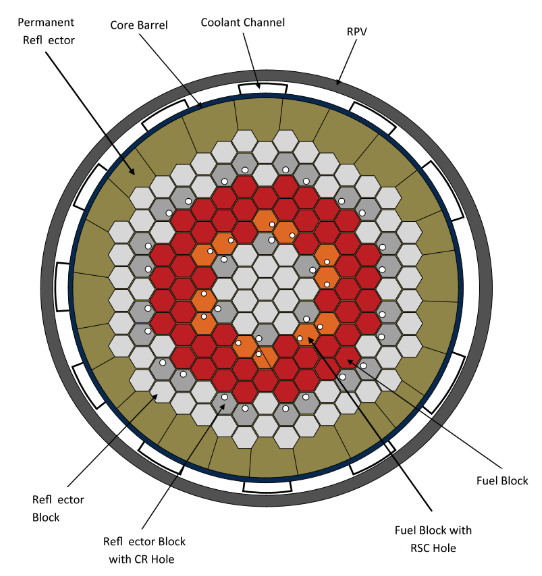
\includegraphics[width=0.45\textwidth]{figures/radial-layout.png}
    }
    \subfloat[Core axial layout. Image reproduced from \cite{oecd_nea_benchmark_2017}.\label{fig:layoutb}]{
        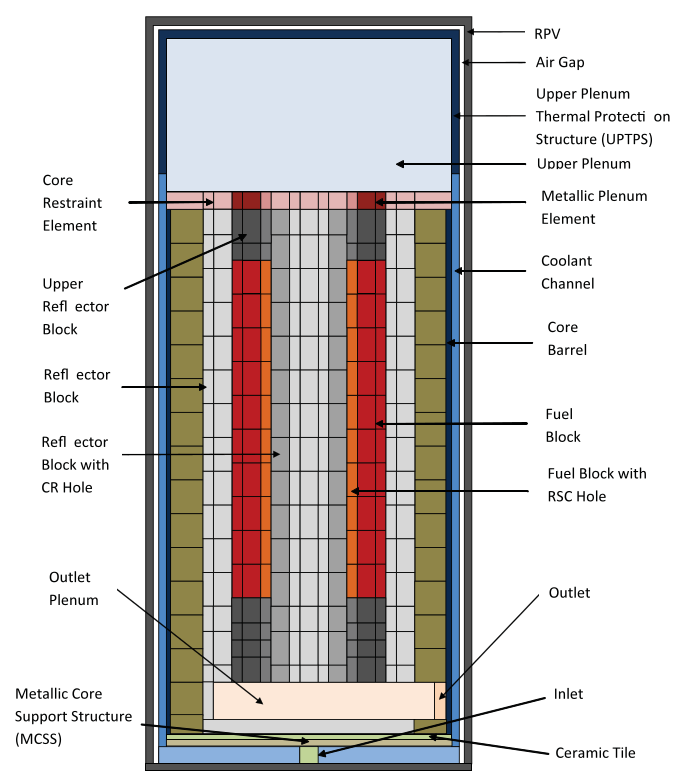
\includegraphics[width=0.45\textwidth]{figures/axial-layout.png}
    }
    \hfill
    \caption{MHTGR reactor layout.}
    \label{fig:layout}
\end{figure}

% \begin{figure}[htbp!]
%   \centering
%   \begin{subfigure}[t]{0.4\textwidth}
%     \centering
%     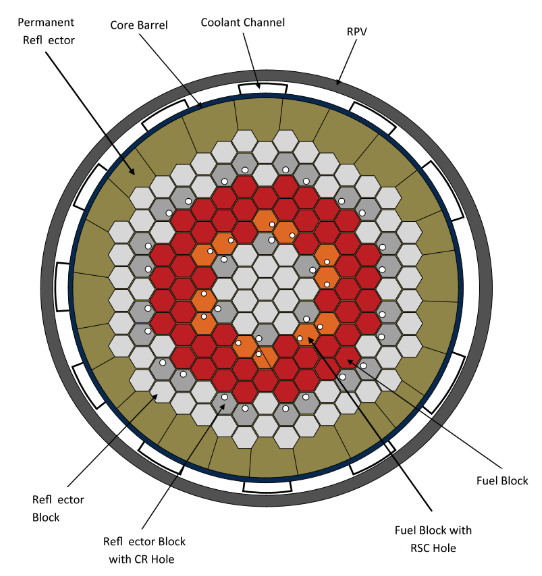
\includegraphics[width=0.95\linewidth]{figures/radial-layout.png}
%     \caption{Core radial layout. Image reproduced from \cite{oecd_nea_benchmark_2017}.}
%   \end{subfigure}
%   \begin{subfigure}[t]{0.4\textwidth}
%     \centering
%     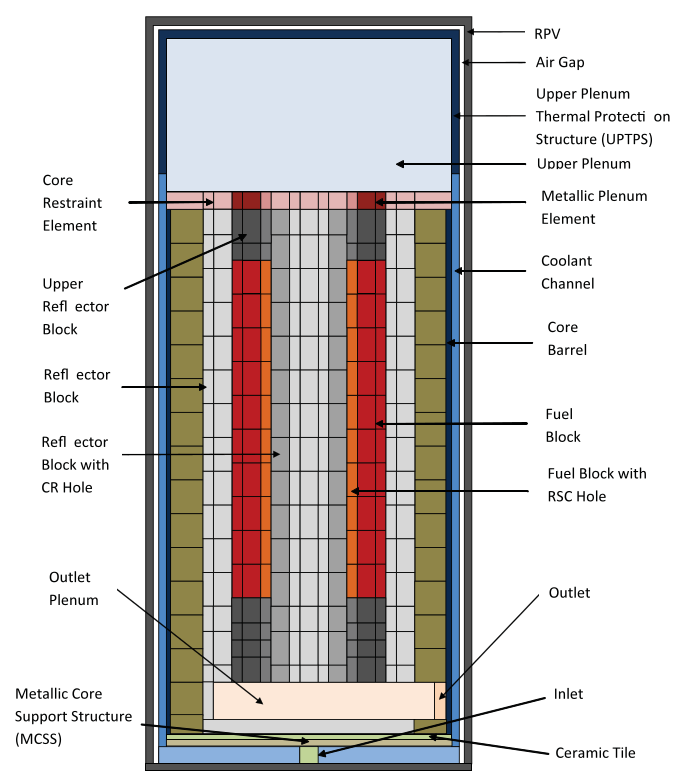
\includegraphics[width=0.95\linewidth]{figures/axial-layout.png}
%     \caption{Core axial layout. Image reproduced from \cite{oecd_nea_benchmark_2017}.}
%     \label{fig:layoutb}
%   \end{subfigure}
%   \hfill
%   \caption{MHTGR reactor layout.}
%   \label{fig:layout}
% \end{figure}

Ten layers of fuel elements stacked on top of each other compose the 66 fuel columns that integrate the active core.
Figure \ref{fig:layoutb} shows an axial view of the reactor.
The core has two types of fuel elements: a standard element and a reserve shutdown element that contains a channel for \gls{RSC}, Figure \ref{fig:fuelassembly}.
Table \ref{tab:element-characteristics} specifies the details of the MHTGR-350 fuel elements.
Twelve columns in the core contain \gls{RSC} channels for reserve shutdown borated graphite pellets.
Hoppers above the core house the pellets, and if the \glspl{CR} become inoperable, the pellets drop into the channels \cite{oecd_nea_benchmark_2017}.

\begin{figure}[htbp!]
  \centering
    \subfloat[Standard fuel assembly. Image reproduced form \cite{tak_numerical_2008}.]{
        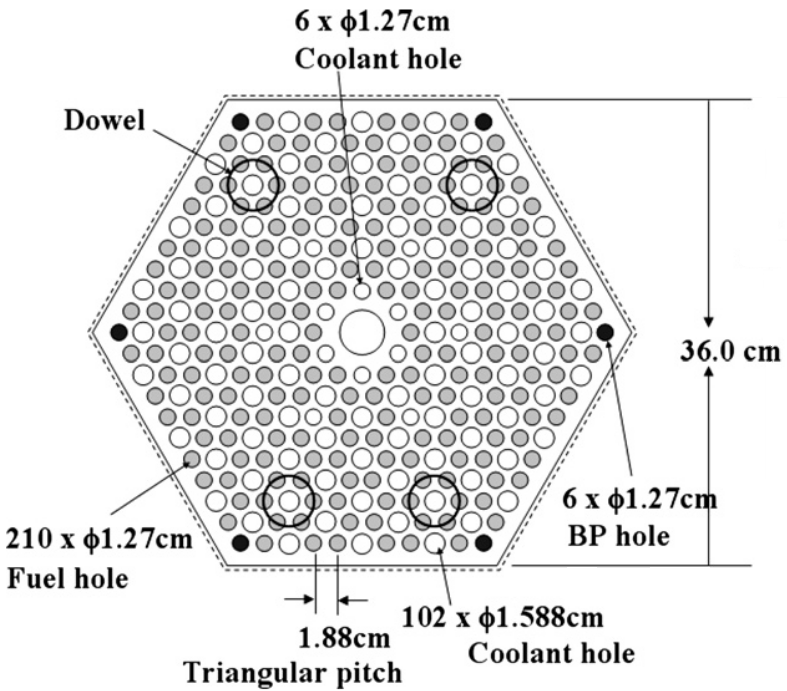
\includegraphics[width=0.45\textwidth]{figures/fuel-assembly}
    }
    \subfloat[RSC fuel assembly. Image reproduced form \cite{tak_practical_2012}.]{
        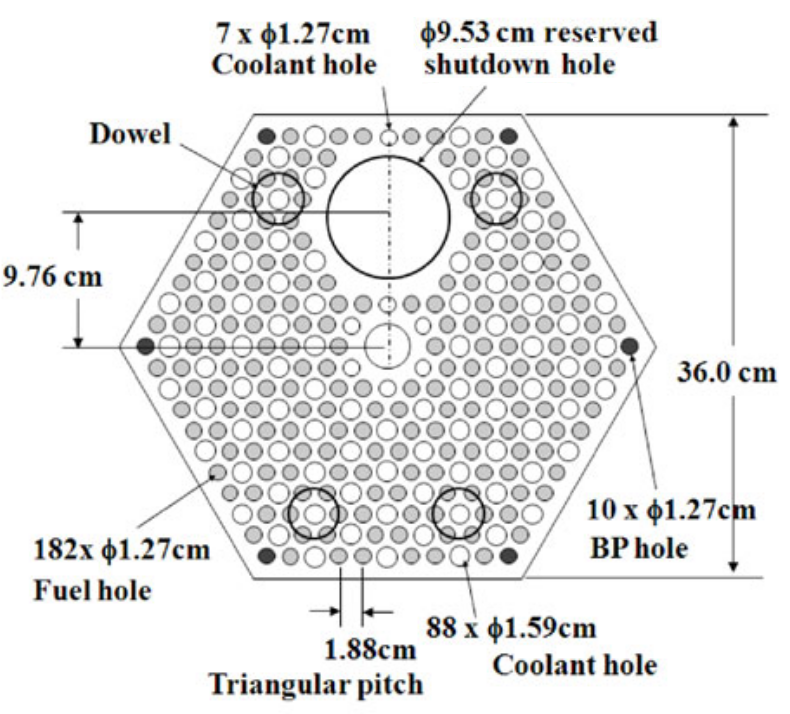
\includegraphics[width=0.45\textwidth]{figures/fuel-assembly-rsc}
    }
  \hfill
    \caption{MHTGR-350 fuel assembly layout.}
  \label{fig:fuelassembly}
\end{figure}

\begin{table}[htbp!]
\centering
      \caption{MHTGR350 fuel element characteristics \cite{oecd_nea_benchmark_2017}.}
      \label{tab:element-characteristics}
    \begin{tabular}{@{}l S[table-format=2.2] c}
    \toprule
    \multicolumn{1}{c}{Shared characteristics} & \multicolumn{1}{c@{}}{Value} & \multicolumn{1}{c@{}}{Units} \\
    \midrule
  Block pitch (flat-to-flat)       & 36      & cm       \\
  Fuel length                      & 79.3    & cm       \\
  Fuel handling diameter           & 3.5     & cm       \\
  Fuel handling length             & 26.4    & cm       \\
  RSC hole diameter                & 9.525   & cm       \\
  RSC center to assembly center    & 9.756   & cm       \\
  Fuel/coolant pitch               & 1.879   & cm       \\
  Fuel hole radius                 & 0.635   & cm       \\
  Compacts per fuel hole           & \multicolumn{1}{c@{}}{15}    & -        \\
  Large coolant hole radius        & 0.794   & cm       \\
  Small coolant hole radius        & 0.635   & cm       \\
  LBP hole radius                  & 0.635   & cm       \\
  Block graphite density           & 1.85    & g/cm$^3$ \\
  \midrule

      \multicolumn{1}{c}{Standard element} &  &  \\

  \midrule
  Number of large coolant holes    & \multicolumn{1}{c@{}}{120}   & -        \\
  Number of small coolant holes    & \multicolumn{1}{c@{}}{6}     & -        \\
  Number of fuel holes             & \multicolumn{1}{c@{}}{210}   & -        \\
  \midrule

      \multicolumn{1}{c}{RSC element} &  &  \\

  \midrule
  Number of large coolant holes    & \multicolumn{1}{c@{}}{88}    & -        \\
  Number of small coolant holes    & \multicolumn{1}{c@{}}{7}     & -        \\
  Number of fuel holes             & \multicolumn{1}{c@{}}{186}   & -        \\
    \bottomrule
    \end{tabular}
\end{table}

% Fuel assemblys and triso particles
The fuel elements contain blind holes for fuel compacts and full-length channels for helium coolant flow.
Table \ref{tab:compact} specifies the details of the TRISO particle and fuel compact designs of the \gls{MHTGR}-350.

\begin{table}[htbp!]
\centering
    \caption{TRISO and fuel compact characteristics \cite{oecd_nea_benchmark_2017}.}
    \label{tab:compact}
    \begin{tabular}{@{}l S[table-format=2.1] c}
    \toprule
    \multicolumn{1}{c}{Characteristic} & \multicolumn{1}{c@{}}{Value} & \multicolumn{1}{c@{}}{Units} \\
    \midrule
  Fuel                             & UC$_{0.5}$O$_{1.5}$   & -        \\
  Enrichment (average)             & 15.5                  & wt\%     \\
  Packing fraction (average)       & 0.35                  & -        \\
  Kernel radius                    & 0.02125               & cm       \\
  Buffer radius                    & 0.03125               & cm       \\
  IPyC radius                      & 0.03475               & cm       \\
  SiC radius                       & 0.03825               & cm       \\
  OPyC radius                      & 0.04225               & cm       \\
  Compact radius                   & 0.6225                & cm       \\
  Compact gap radius               & 0.6350                & cm       \\
  Compact length                   & 4.9280                & cm       \\
  Kernel density                   & 10.50                 & g/cm$^3$ \\
  Buffer density                   & 1.00                  & g/cm$^3$ \\
  IPyC density                     & 1.90                  & g/cm$^3$ \\
  SiC density                      & 3.20                  & g/cm$^3$ \\
  OPyC density                     & 1.90                  & g/cm$^3$ \\
  Compact matrix density           & 1.74                  & g/cm$^3$ \\
    \bottomrule
    \end{tabular}
\end{table}

% Reactivity control
A combination of \gls{LBP} and \glspl{CR} controls the core reactivity.
The \gls{LBP} consists of \gls{B4C} granules dispersed in graphite compacts.
The current design uses six \gls{LBP} rods per element.
Table \ref{tab:LBP} displays the characteristics of the \gls{LBP} compacts.
The reactor has 30 \glspl{CR}.
Six of them are start-up \glspl{CR}, and their location is the inner reflector.
The remaining 24 are operating \glspl{CR} and control the reactivity during power operation and a reactor trip.

\begin{table}[htbp!]
\centering
    \caption{LBP compact characteristics \cite{oecd_nea_benchmark_2017}.}
    \label{tab:LBP}
    \begin{tabular}{@{}l S[table-format=1.4] c}
    \toprule
    \multicolumn{1}{c}{Characteristic} & \multicolumn{1}{c@{}}{Value} & \multicolumn{1}{c@{}}{Units} \\
    \midrule
  Absorber                         & B$_{4}$C              & -         \\
  Packing fraction                 & 0.109                 & -         \\
  Kernel radius                    & 0.0100                & cm        \\
  Buffer radius                    & 0.0118                & cm        \\
  PyC radius                       & 0.0141                & cm        \\
  Compact radius                   & 0.5715                & cm        \\
  Compact gap radius               & 0.6350                & cm        \\
  Rod length                       & 72.187                & cm        \\
  Kernel density                   & 2.47                  & g/cm$^3$  \\
  Buffer density                   & 1.00                  & g/cm$^3$  \\
  PyC density                      & 1.87                  & g/cm$^3$  \\
  Compact matrix density           & 0.94                  & g/cm$^3$ \\
    \bottomrule
    \end{tabular}
\end{table}


\chapter{Neutronics}
\label{ch:neutronics}

This chapter presents several studies that use Moltres as a stand-alone neutronics solver.
The objective of the chapter is to validate Moltres calculation scheme by comparing Moltres results to Serpent and the OECD/NEA MHTGR-350 Benchmark.
This chapter comprehends the following sections: Section \ref{sec:neut-prelim} describes some preliminary studies that help set up Serpent and Moltres simulations, Section \ref{sec:neut-serpent} presents several studies comparing Moltres and Serpent results, Section \ref{sec:ph1e1} discusses Moltres results of Phase I Exercise 1 of the Benchmark, and Section \ref{sec:neutr-conc} concludes the chapter with a summary of the chapter and its key points.

\section{Preliminary studies}
\label{sec:neut-prelim}

This section's purpose is to find the right set up of Serpent and Moltres input files.
Section \ref{sec:homo-hetero} focuses on the materials definition in Serpent input file for obtaining the group constants for Moltres.
Section \ref{sec:setup} analyzes different ways to set up Moltres input files.

\subsection{Homogeneous vs. heterogeneous isotope distribution}
\label{sec:homo-hetero}

This section determines the proper way to treat the fuel compact heterogeneities in Serpent.
This study modeled in Serpent two different material distributions in a fuel compact: a homogeneous distribution of the isotopes and a heterogeneous distribution that explicitly modeled the TRISO particles.
The study used a hexagonal unit cell model that included the fuel compact, a helium gap, and the surrounding graphite, exhibited in Figure \ref{fig:compact-model}.
Table \ref{tab:compact} specifies the model input parameters.
The material temperature was 1200K, a case that represents the \gls{HFP} core state.
The Serpent simulations included 5$\times 10^4$ neutrons per cycle, 500 active cycles, and 50 inactive cycles for the calculations.
The homogeneous distribution simulation took 1.73 minutes and the heterogeneous distribution simulation 2.21 minutes using 256 cores --- the heterogeneous calculation took 28$\%$ longer.

\begin{figure}[htbp!]
  \centering
    \subfloat[Homogeneous isotope distribution in the fuel compact.]{
        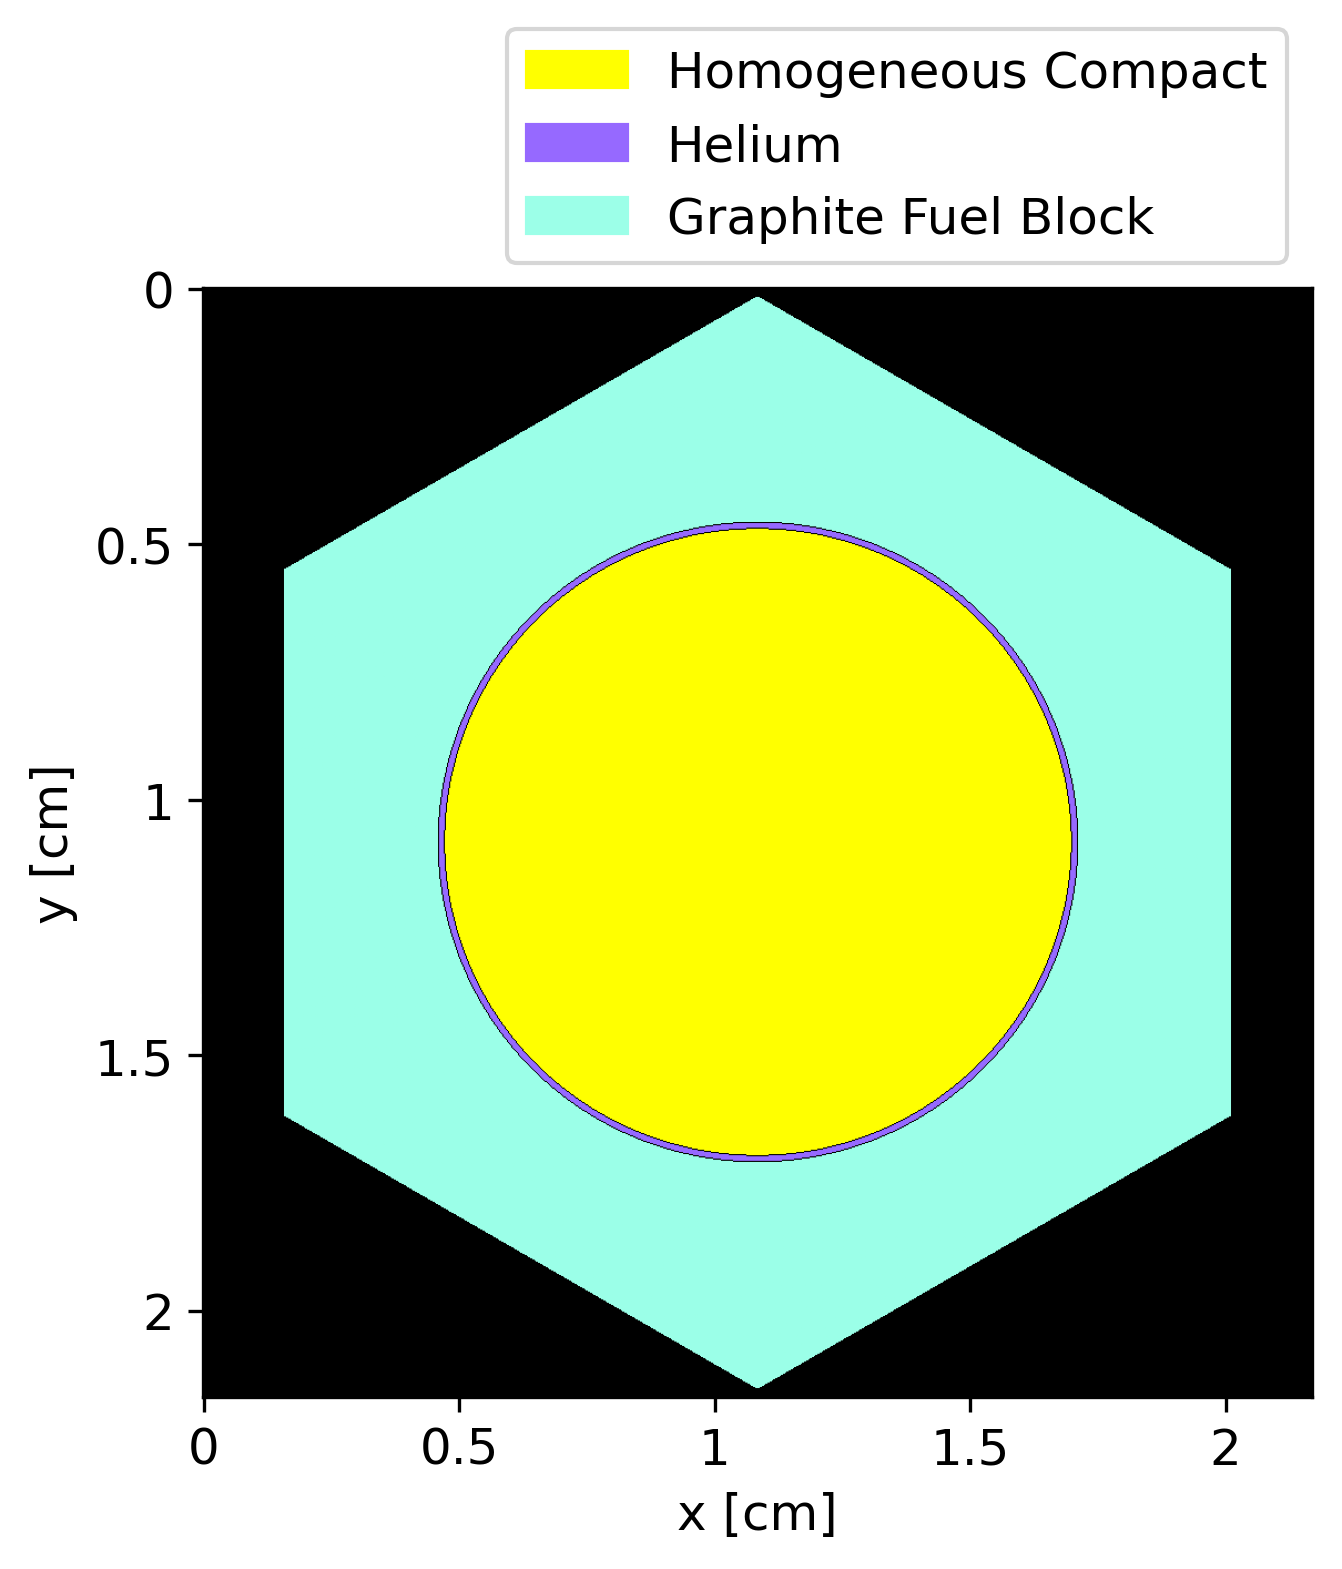
\includegraphics[width=0.45\textwidth]{figures-neutronics/compact-homo}
    }
    \subfloat[Explicit model of the TRISO particles in the fuel compact.]{
        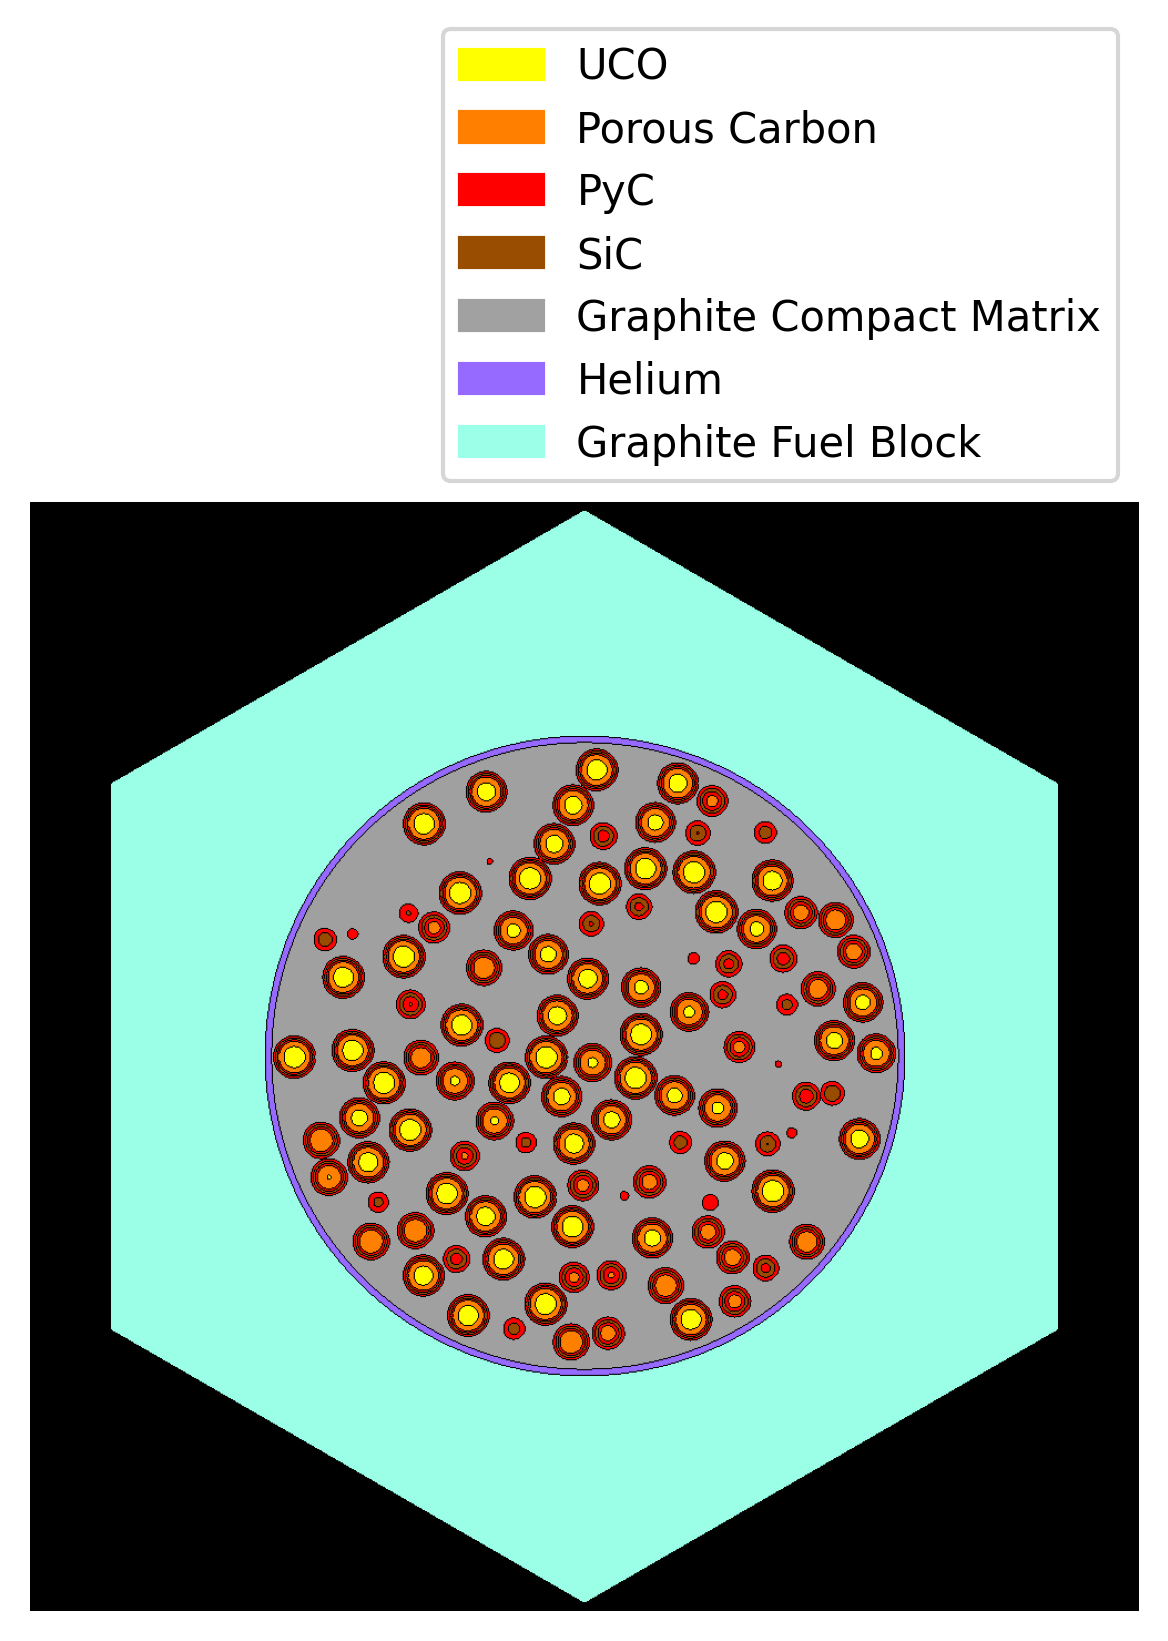
\includegraphics[width=0.45\textwidth]{figures-neutronics/compact}
    }
  \hfill
  \caption{Comparison of different Serpent models of the fuel compact.}
  \label{fig:compact-model}
\end{figure}

The \gls{Keff} was 1.17527 $\pm$ 0.00021 for the homogeneous distribution and 1.25107 $\pm$ 0.00020 for the heterogeneous distribution.
Serpent generated the group constants using the three energy group structure [0, 2.38eV, 111keV, 20MeV].
Using the heterogeneous distribution as the reference, a python script calculated the relative error of some of the group constants in an eigenvalue calculation.
The evaluated parameters were $D_g$, $\Sigma^r_g$, $\nu\Sigma^f_g$, and $\chi^t_g$ (see Equation \ref{eq:diffusion-eig}).
Figure \ref{fig:param-comparison} displays the relative errors for $\Sigma^r_g$ and $\nu\Sigma^f_g$, which were the group constants that changed the most.
The figure does not include $D_g$ and $\chi^t_g$ because their relative errors were less than 1$\%$.
The relative errors of $\Sigma^r_g$ and $\nu\Sigma^f_g$ were less than 6$\%$.

\begin{figure}[htbp!]
	\centering
	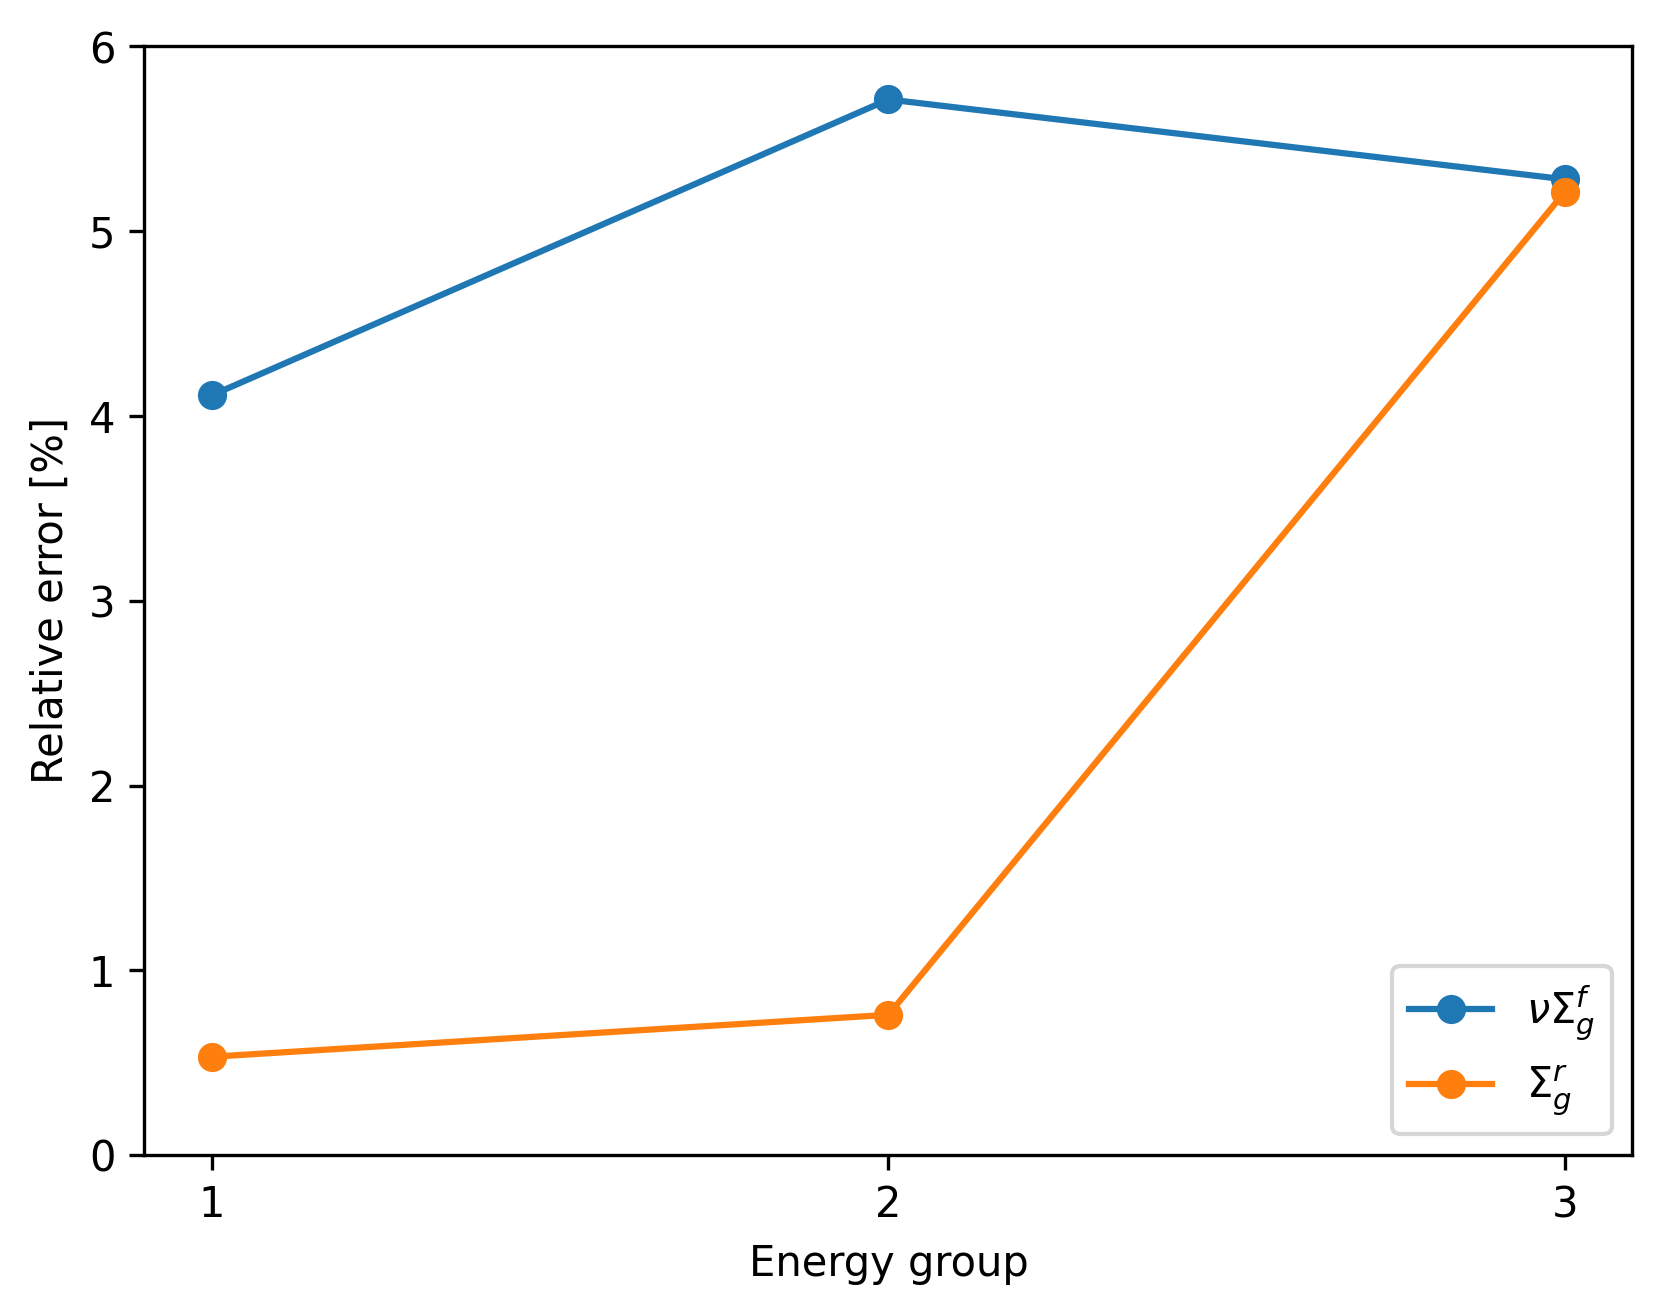
\includegraphics[width=0.43\linewidth]{figures-neutronics/param-comparison}
	\hfill
	\caption{Relative error of the group constants generated with a homogeneous isotope distribution vs explicit TRISO modeling.}
	\label{fig:param-comparison}
\end{figure}

The results show that the homogenization of the fuel compact isotopes decreases the multiplication factor considerably.
The impact on the group constants does not seem to be substantial; however, the multiplication factor's considerable difference suggests that the combined effect of the small variations in the group constants is significant.
Based on these results, Serpent models the TRISO particles explicitly for generating the group constants in the following sections.

\subsection{Problem set-up}
\label{sec:setup}

% Diffusion calculations: homo vs hetero in LWRs
Diffusion calculations necessitate a spatial homogenization of the group constants.
Depending on the desired level of detail, the type of homogenization could vary.
For example, in PWR core calculations, the homogenization in space could be per assembly or pin-by-pin \cite{krebs_calculational_1990}.
In a per-assembly homogenization, the diffusion solver represents the assembly as a single material neutronically (we will refer to diffusion calculations using this type as homogeneous calculations).
A pin-by-pin homogenization treats the pin or assembly heterogeneities, yielding a more detailed neutronic representation of the fuel assembly (we will refer to diffusion calculations of this type as heterogeneous calculations).

% Previous works using Moltres
Previous work \cite{lindsay_introduction_2018}\cite{pater_multiphysics_2019} used Moltres for simulating \glspl{MSR}, which allow for heterogeneous calculations.
In those calculations, the authors defined two materials in Moltres input files: the moderator and the fuel.
For such a configuration, a moderator mesh node holds the neutronics and temperature information only of the moderator.
The same is true in the fuel.
% On the other hand, a homogeneous calculation would not differentiate between moderator and fuel and would hold the information of both materials in each node.

% What I did in this section:
Keeping in mind Moltres proven capabilities, this work aimed for a heterogeneous calculation of a prismatic \gls{HTGR}.
For this study, Serpent modeled a fuel column of the MHTGR-350 and generated the group constants.
Figure \ref{fig:fuelcolumn} displays the Serpent model geometry.
Serpent generated the group constants for three materials: moderator, coolant, and fuel compact.
The Serpent simulations included 5$\times 10^5$ neutrons per cycle, 400 active cycles, and 100 inactive cycles for the calculations.
% The \gls{Keff} was 1.41933.
Taking advantage of the problem's symmetry, Moltres modeled only $1/12^{th}$ of the fuel column shown in Figure \ref{fig:fuelcolumn}.
I made the geometry and mesh using Gmsh \cite{geuzaine_gmsh_2020}.
The diffusion calculation had 1.84$\times 10^5$ \glspl{DoF} per energy-group.

\begin{figure}[htbp!]
	\centering
    \subfloat[Serpent model geometry.]{
        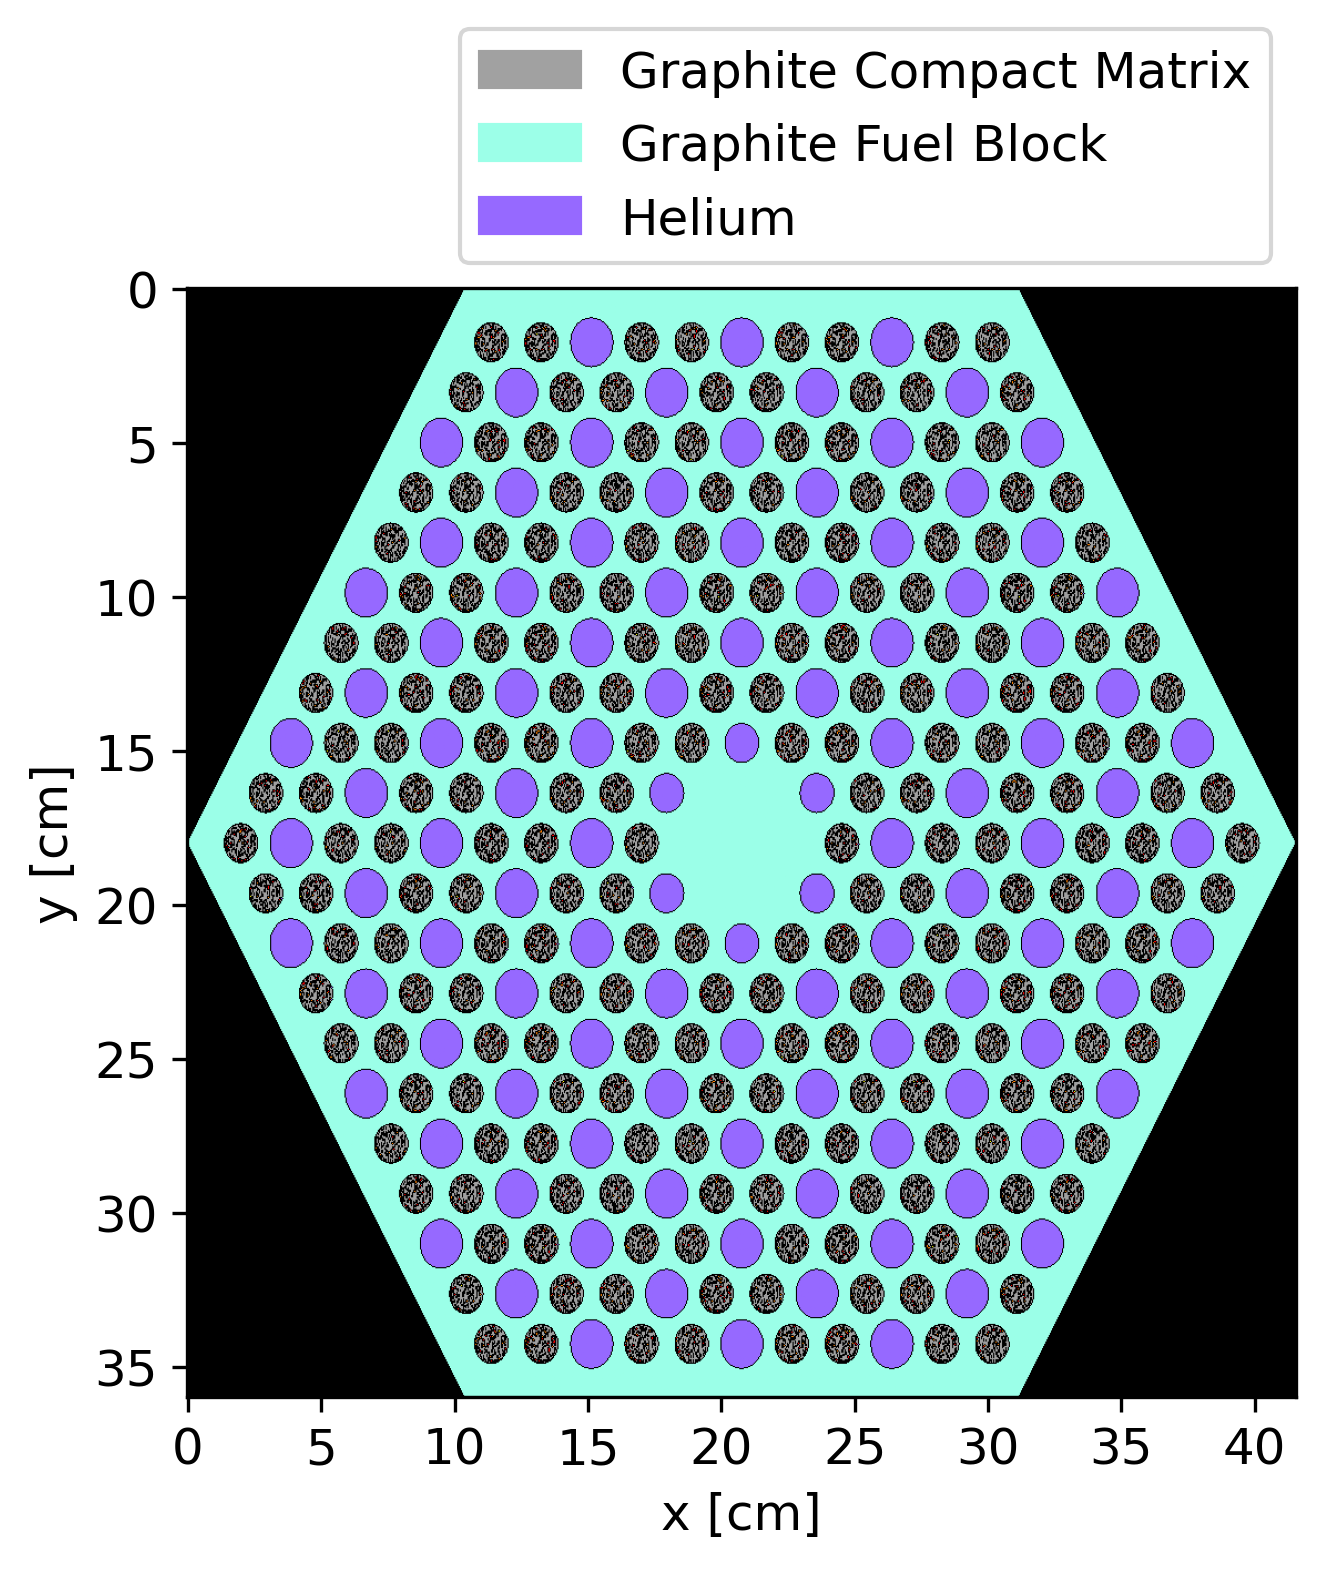
\includegraphics[width=0.35\textwidth]{figures-neutronics/standard}
    }
    \subfloat[Moltres model geometry.]{
        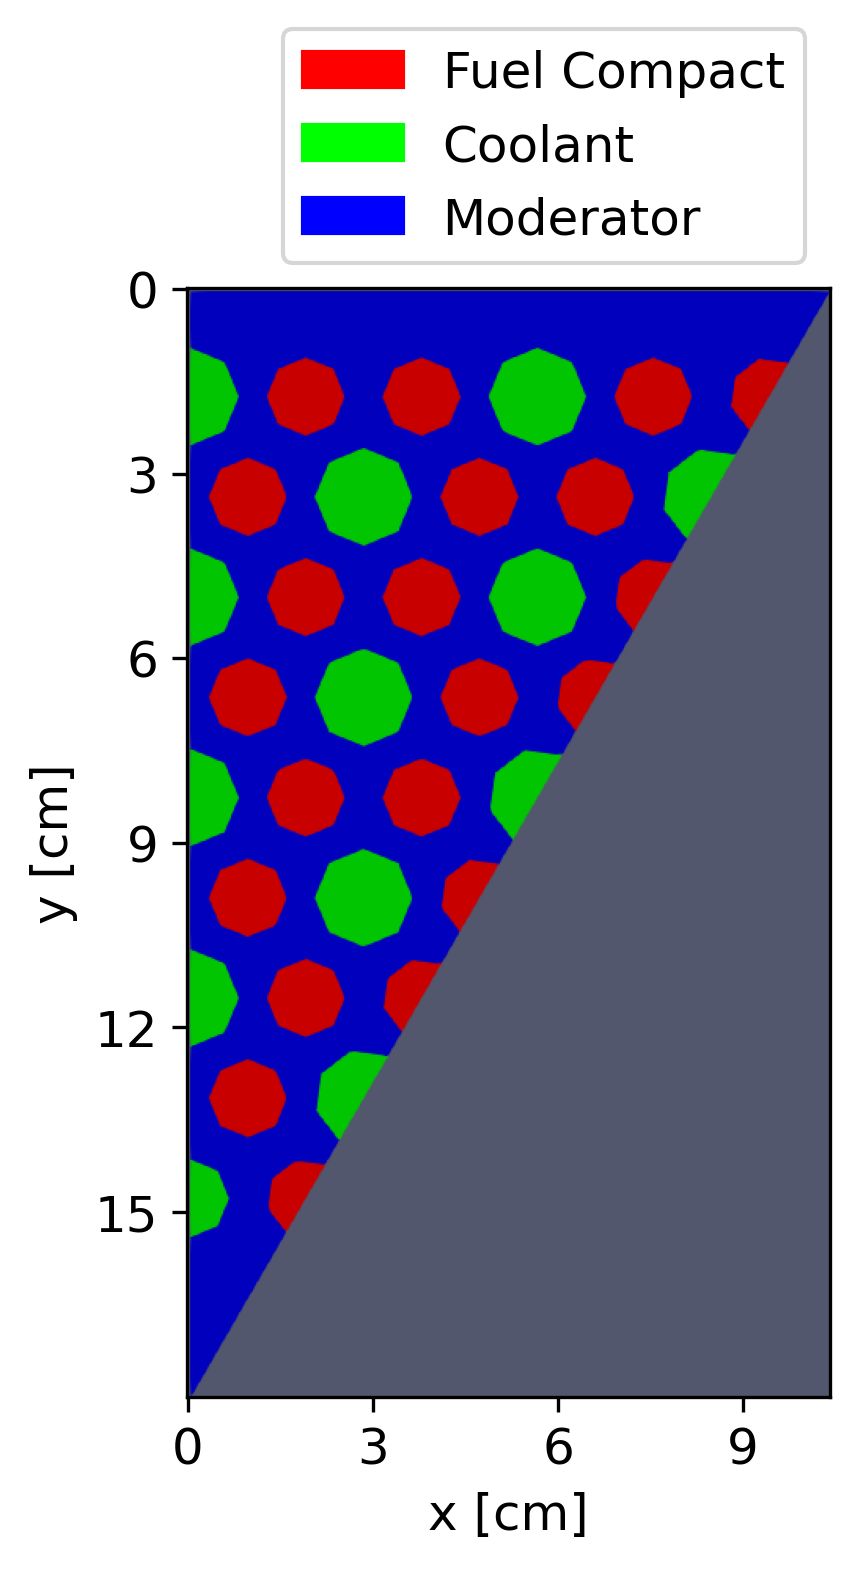
\includegraphics[width=0.22\textwidth]{figures-neutronics/3D-assembly-30deg-reflec-meshB2}
    }
	\hfill
    \caption{Fuel column of the MHTGR-350. $xy$-plane in the active core region.}
	\label{fig:fuelcolumn}
\end{figure}

Moltres simulation obeyed an eigenvalue convergence tolerance of 1$\times$10$^{-8}$, defined by equation \ref{eq:moltres-tol}

\begin{align}
   & \frac{k^{(n)}-k^{(n-1)}}{k^{(n)}} < \varepsilon \label{eq:moltres-tol}
   \intertext{where}
   & k^{(n)} = \mbox{eigenvalue at iteration $n$ } [-] \notag \\
   & \varepsilon = \mbox{convergence tolerance } [-]. \notag
\end{align}

The calculation used two energy groups with the structure [0, 0.625eV, 20MeV].
The eigenvalue calculation did not converge.
Although several factors could contribute to this behavior, I focused on the validity of the diffusion calculations in this system.

% Diffusion validity see bu1/tools-bu.txt
In diffusion theory, the current density $J$ is proportional to the gradient of the flux, see equation \ref{eq:diff} \cite{leppanen_development_2007}.
\begin{align}
   & J = - D \nabla \phi \label{eq:diff} \\
   \intertext{where}
   & J = \mbox{current density } [n \cdot cm^{-2} \cdot s^{-1}] \notag \\
   & D = \mbox{diffusion coefficient } [cm] \notag \\
   & \phi = \mbox{neutron flux } [n \cdot cm^{-2} \cdot s^{-1}]. \notag
\end{align}

This approximation relies on the following assumptions:
\begin{itemize}
	\item the angular flux does not depend strongly on the angular variables,
	\item the fission source is isotropic,
	\item the time derivative of the current density is small compared to the mean collision time,
	\item and the anisotropic energy-transfer due to scattering is negligible in group-to-group scattering.
\end{itemize}

More detailed studies of the transport equation indicate that the following cases violate the assumption of a weak angular dependence \cite{duderstadt_nuclear_1976}:
\begin{itemize}
    \item regions near vacuum boundaries and low-density material regions,
    \item regions near strongly absorbing media,
    \item and regions near localized sources.
\end{itemize}

The diffusion theory applies best to geometries consisting of large homogeneous regions where the flux gradient is small.
This is the case for material regions whose geometrical scales are considerably larger than the neutron mean free path.
For this reason, Table \ref{tab:mfp} compares the neutron mean free path in the different fuel assembly materials.
The mean free path in the fuel compact and the moderator are in the order of the centimeters.
In the coolant, the mean free path magnitude is comparable to the fuel column dimensions.
These results suggest that a heterogeneous diffusion calculation of the prismatic fuel column challenges some of the diffusion theory assumptions.

\begin{table}[htbp!]
  \centering
  \caption{Neutron mean free path in different materials. Values expressed in $cm$.}
  \begin{tabular}{l|cccc}
  \toprule
              & Fuel compact  & Moderator  & Coolant  & Homogeneous fuel \\
  \midrule
  Fast  		  & 2.71 & 2.70 & 1137.31 & 3.37 \\
  Thermal		  & 2.22 & 2.36 & 1945.49 & 2.89 \\
  \bottomrule
  \end{tabular}
  \label{tab:mfp}
\end{table}

Next, I conducted a feasibility study for the homogeneous calculation of the fuel assembly in Moltres.
Serpent calculated the homogeneous group constants of the fuel assembly, see equation \ref{eq:diffusion-eig}, by homogenizing the fuel, coolant, and moderator.
This material's mean free path is in the order of the centimeters, Table \ref{tab:mfp}.
Next, Moltres used the homogeneous group constants to carry out an eigenvalue calculation.
Comparing Moltres results with Serpent results, Serpent's \gls{Keff} was 1.41942 $\pm$ 0.00007 while Moltres' was 1.40788.
Moltres eigenvalue is smaller than Serpent's eigenvalue.
% This difference is possibly due to the lack of treatment of the anisotropic term in the scattering cross-section.
Additionally, Figure \ref{fig:prelim} displays a comparison between the axial flux in the fuel column obtained with Serpent vs. Moltres.
Serpent's flux is the average value of the flux in each bin, while Moltres flux is the point-wise flux over the $z$-axis
\begin{align}
  & \phi_s(z) = \frac{\int_{\Delta V} \phi(x,y,z) dV}{\Delta V} \label{eq:serpent-flux} \\
  & \phi_m(z) = \phi_m(x,y,z)   \label{eq:moltres-flux}
  \intertext{where}
  & \phi_s(z) = \mbox{Serpent axial flux } [n \cdot cm^{-2} \cdot s^{-1}] \notag \\
  & \Delta V = \mbox{Volume of the detector bins } [cm^3] \notag \\
  & \phi_m(z) = \mbox{Moltres axial flux } [n \cdot cm^{-2} \cdot s^{-1}]. \notag
\end{align}

The fluxes are similar in shape and magnitude.
% Conclusion
I emphasize that this was a feasibility study.
The following sections present a more in-depth analysis of more detailed results.
Based on these results and discussion, I conducted homogeneous calculations using Moltres in the following sections.

\begin{figure}[htbp!]
	\centering
    \subfloat[Serpent axial flux.]{
        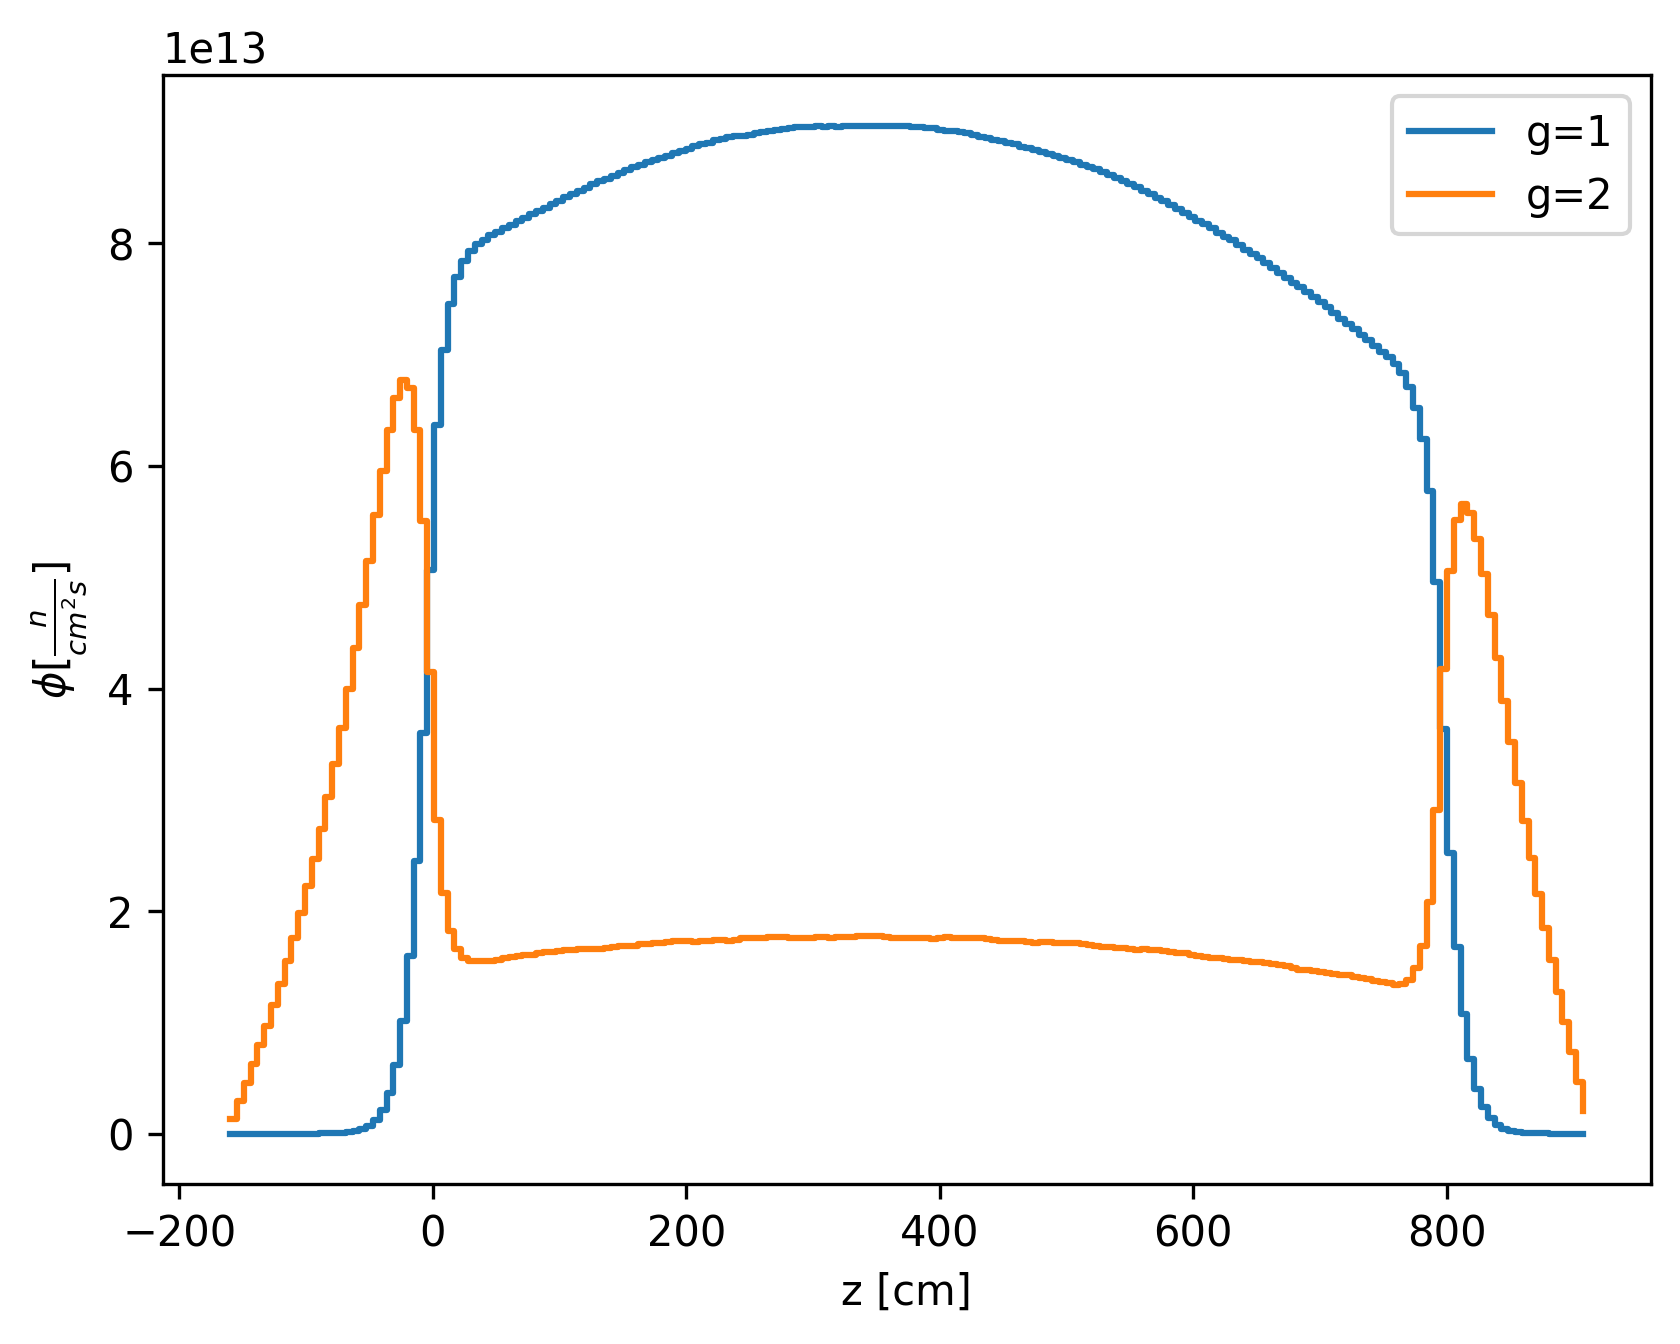
\includegraphics[width=0.45\textwidth]{figures-neutronics/standard-column-detector-Axial}
    }
    \subfloat[Moltres axial flux.]{
        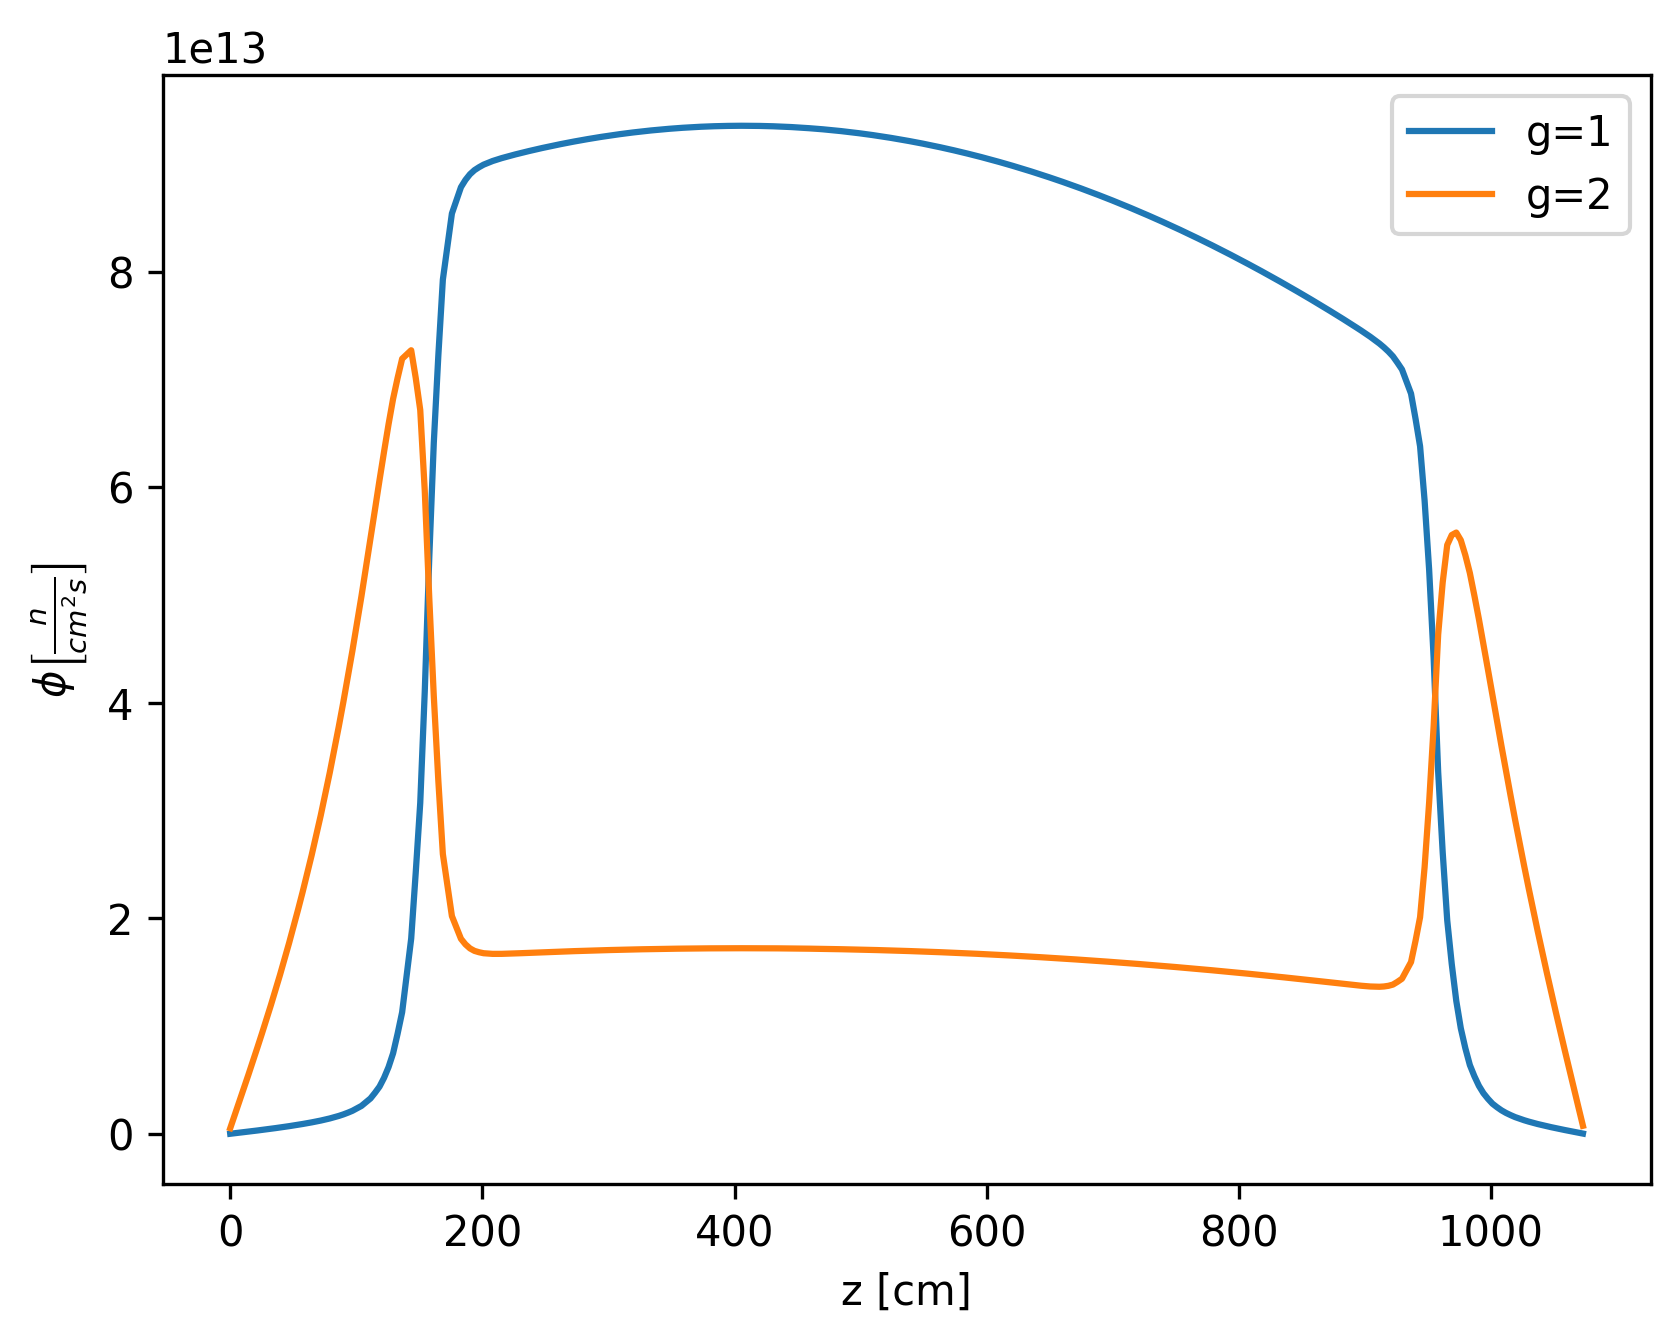
\includegraphics[width=0.45\textwidth]{figures-neutronics/homo-fuel}
    }
	\hfill
  \caption{Comparison of the two group axial flux in the fuel column.}
	\label{fig:prelim}
\end{figure}

\section{Serpent-Moltres comparison}
\label{sec:neut-serpent}

In this section, Serpent modeled a fuel column and the full-core of the MHTGR-350.
Serpent obtained the homogenized group constants that served as input to Moltres.
The following sections compare Moltres and Serpent results as a validation exercise.

\subsection{Fuel column}

This section investigats the effects of the energy group structure on the diffusion simulations.
I conducted two analyses: first, I varied the number of energy groups, second, I varied the energy group structures with a constant number of energy groups.
To reduce the computational expense, we narrowed down our focus to a fuel column of the MHTGR-350, Figure \ref{fig:fuelcolumn}.
% The fuel column includes the bottom and top reflectors.
Tables \ref{tab:element-characteristics} and \ref{tab:compact} specify the model input parameters.

The first step in the calculation was to obtain the group constants using Serpent.
Figure \ref{fig:fuelcolumn} displays the axial layout of the model.
Serpent's model did not consider the fuel handling holes or the bottom and top reflectors' coolant channels for simplicity.
\glspl{HTGR} use burnable poisons to reduce the power peaking factors in various active core regions.
Some reactors have burnable poisons in the rings closer to the reflectors, and no burnable poisons in the middle rings.
This characteristic motivated the analysis of two cases: one fuel column that does not have burnable poisons and one that does.
The burnable poisons' locations are the six corners of the fuel assembly, Figure \ref{fig:fuelassembly}.
The material temperatures were 600 and 1200K, cases that represent the \gls{CZP} and the \gls{HFP} core states.
The Serpent simulations included 4$\times 10^5$ neutrons/cycle, 360 active cycles, and 40 inactive cycles for the calculations.

Taking advantage of the problem's symmetry, Moltres modeled only $1/12^{th}$ of the homogenized fuel column.
I made the geometry and mesh, which had 3.71 $\times 10^4$ elements and 2.29 $\times 10^4$ nodes, using Gmsh.
The diffusion calculations had 2.29 $\times 10^4$ \glspl{DoF} per energy-group.
The Moltres input files set an eigenvalue and a flux convergence tolerance of 1$\times$10$^{-8}$.
Moltres calculations used the different energy group structures listed in Table \ref{tab:energygroups}.

\begin{table}[htbp!]
  \centering
  \caption{Energy group structure \cite{iaea_evaluation_2003}.}
  \begin{tabular}{S[table-format=2.2e-1]|llllllllllll}
  \toprule
                      & \multicolumn{12}{c}{Group structure} \\
  \multicolumn{1}{c|}{Upper boundary [eV]} & 26    & 21   & 18   & 15a & 15b & 15c & 15d & 15e   & 12  & 9  & 6  & 3 \\
  \midrule
  1.49e+07            & 1     & 1    & 1    & 1   & 1   & 1   & 1   & 1     & 1   & 1  & 1  & 1 \\ 
  7.41e+06            & 2     &      &      &     &     &     &     &       &     &    &    &   \\ 
  3.68e+06            & 3     & 2    & 2    & 2   & 2   & 2   & 2   & 2     & 2   &    &    &   \\ 
  6.72e+05            & 4     &      &      &     &     &     &     &       &     &    &    &   \\ 
  1.11e+05            & 5     & 3    & 3    & 3   & 3   & 3   & 3   & 3     & 3   & 2  & 2  & 2 \\ 
  1.93e+04            & 6     & 4    & 4    & 4   & 4   &     &     &       & 4   &    &    &   \\ 
  3.35e+03            & 7     &      &      &     &     &     &     &       &     &    &    &   \\ 
  1.58e+03            & 8     & 5    & 5    &     &     & 4   &     &       &     &    &    &   \\ 
  7.48e+02            & 9     & 6    & 6    & 5   & 5   &     & 4   & 4     & 5   & 3  &    &   \\ 
  2.75e+02            & 10    & 7    & 7    & 6   & 6   & 5   &     &       & 6   & 4  &    &   \\ 
  1.30e+02            & 11    & 8    & 8    & 7   & 7   &     & 5   & 5     & 7   & 5  & 3  &   \\ 
  6.14e+01            & 12    & 9    &      &     & 8   & 6   &     &       &     &    &    &   \\ 
  2.90e+01            & 13    & 10   & 9    & 8   & 9   &     & 6   & 6     &     &    &    &   \\ 
  1.37e+01            & 14    & 11   & 10   & 9   &     &     &     &       & 8   & 6  &    &   \\ 
  8.32e+00            & 15    & 12   & 11   & 10  & 10  & 7   & 7   & 7     & 9   &    &    &   \\ 
  5.04e+00            & 16    &      &      &     &     &     &     &       &     &    &    &   \\ 
  2.38e+00            & 17    & 13   & 12   & 11  & 11  & 8   & 8   & 8     & 10  & 7  & 4  & 3 \\ 
  1.29e+00            & 18    & 14   &      &     &     &     &     &       &     &    &    &   \\ 
  6.50e-01            & 19    & 15   & 13   & 12  & 12  & 9   & 9   & 9     & 11  & 8  & 5  &   \\ 
  3.50e-01            & 20    & 16   &      &     &     & 10  & 10  &       &     &    &    &   \\ 
  2.00e-01            & 21    & 17   & 14   & 13  & 13  & 11  & 11  & 10    &     &    &    &   \\ 
  1.20e-01            & 22    &      &      &     &     &     &     & 11    &     &    &    &   \\ 
  8.00e-02            & 23    & 18   & 15   & 14  & 14  & 12  & 12  & 12    &     &    &    &   \\ 
  5.00e-02            & 24    & 19   & 16   &     &     & 13  & 13  & 13    &     &    &    &   \\ 
  2.00e-02            & 25    & 20   & 17   & 15  & 15  & 14  & 14  & 14    & 12  & 9  & 6  &   \\ 
  1.00e-02            & 26    & 21   & 18   &     &     & 15  & 15  & 15    &     &    &    &   \\ 
  \bottomrule
  \end{tabular}
  \label{tab:energygroups}
\end{table}

% Fluxes
To recapitulate, we simulated four operational cases: 
\begin{itemize}
  \item Operational case 1: fuel with no burnable poisons at 600K.
  \item Operational case 2: fuel with no burnable poisons at 1200K.
  \item Operational case 3: fuel with burnable poisons at 600K.
  \item Operational case 4: fuel with burnable poisons at 1200K.
\end{itemize}

% This is very important and I should review it carefully
To compare the results from Serpent and Moltres, we review the three-group axial fluxes found by each of them.
Moltres ran the calculations for 26 energy groups and collapsed the results into three energy groups to facilitate the results' visualization.
Figures \ref{fig:assembly-noLBP-600-flux} to \ref{fig:assembly-LBP-1200-flux} display the axial flux from the Serpent and the Moltres simulations for all cases.
For the operational case 1, the fluxes are close in shape and magnitude.
For the operational case 2, the fluxes look similar.
The flux in Moltres has a straighter shape.
The thermal flux peak in the bottom reflector is bigger.
For the operational case 3, the flux in Moltres has a larger magnitude.
Additionally, the shape of the Moltres flux is concave, while the Serpent flux is convex.
For the operational case 4, the flux in Moltres is larger and more concave than Serpent flux.
Overall, the fluxes in Moltres and Serpent are close in shape and magnitude.

% No LBP 600
\begin{figure}[htbp!]
	\centering
    \subfloat[Serpent neutron flux.]{
        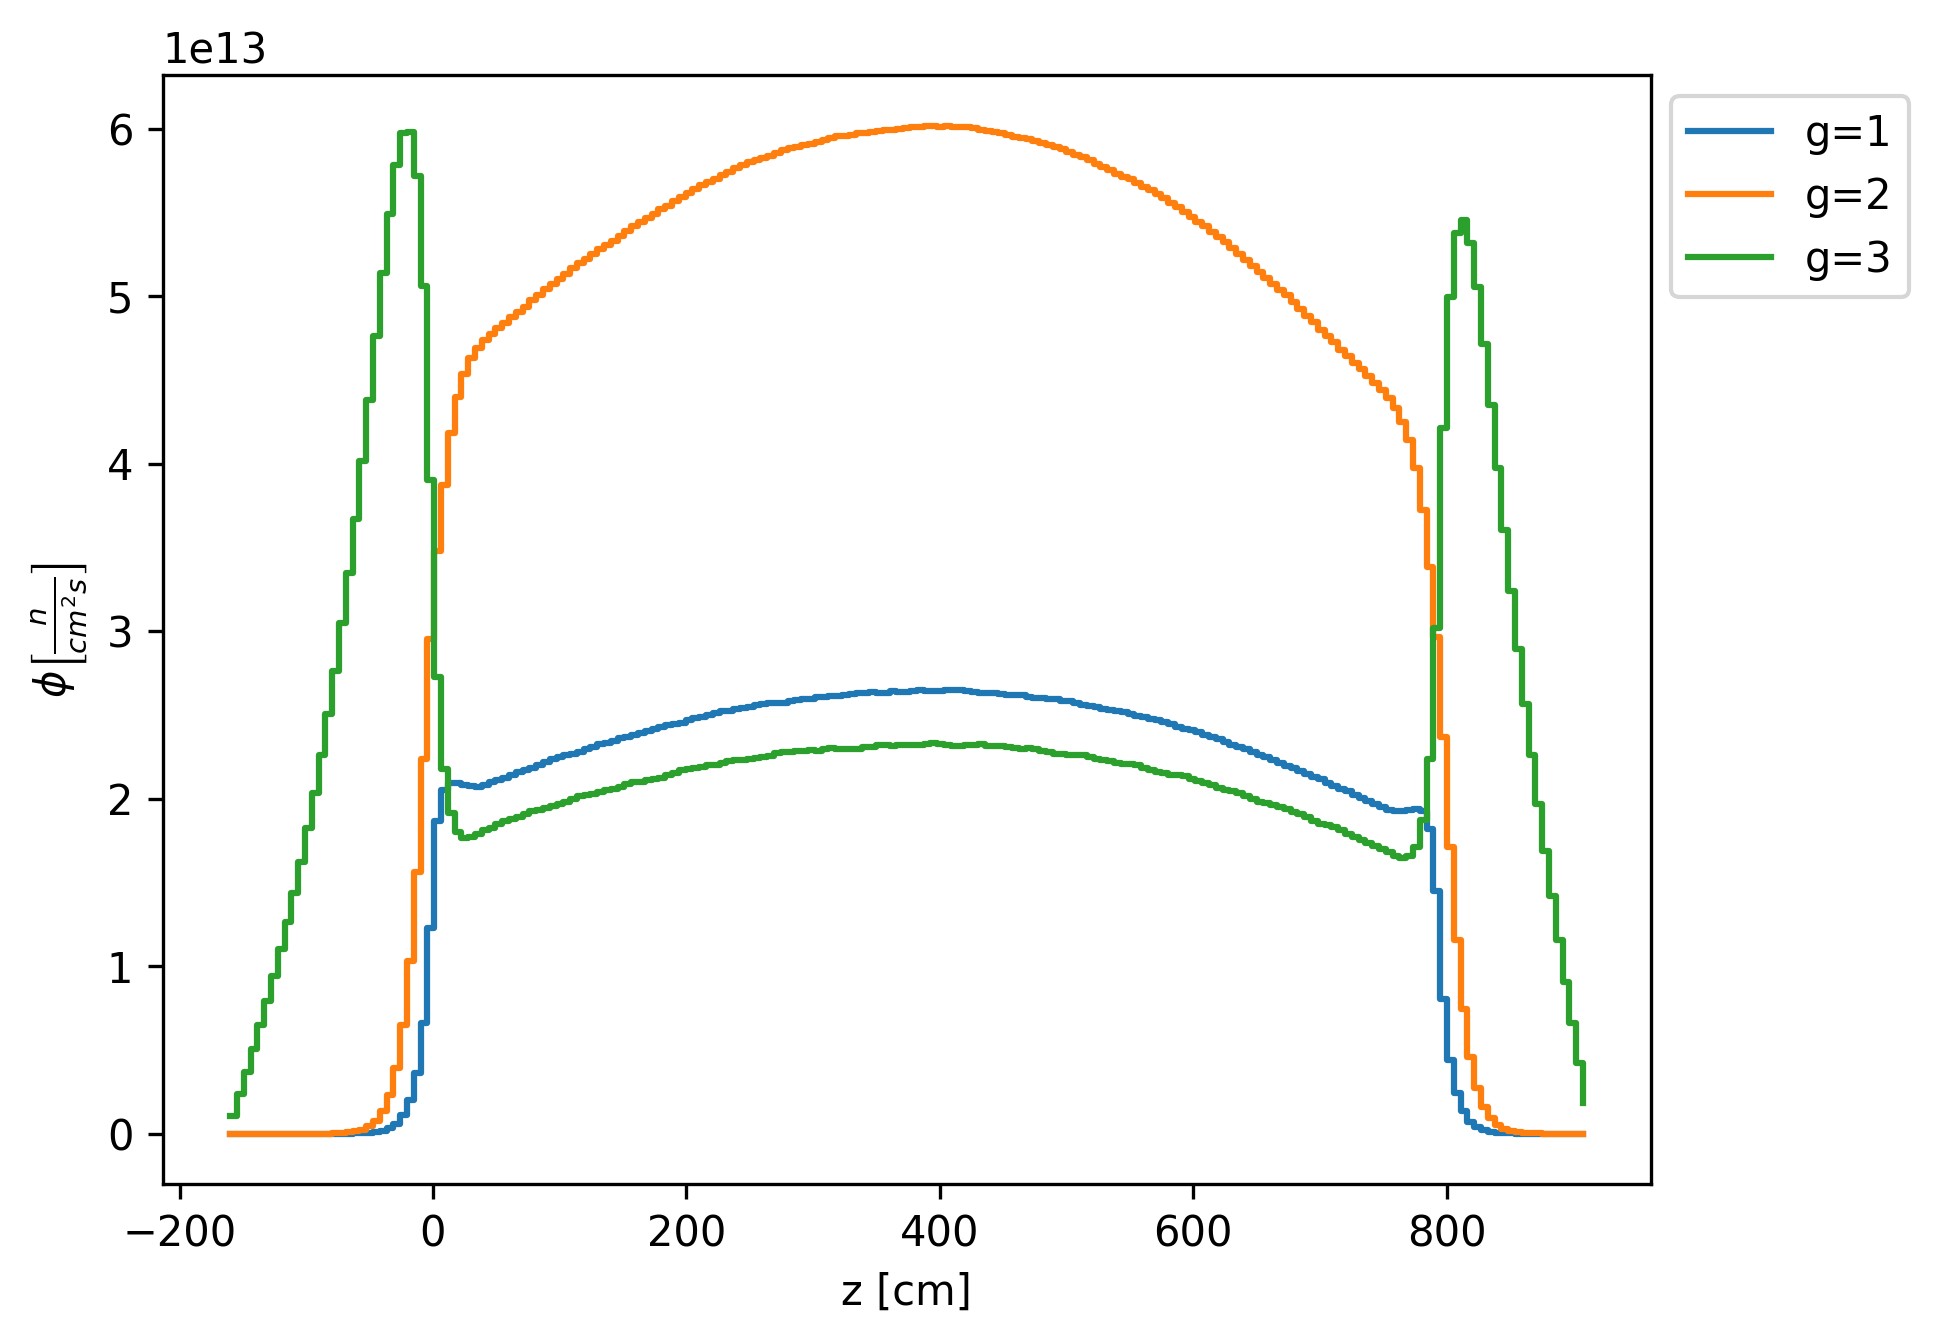
\includegraphics[width=0.45\textwidth]{figures-neutronics/serpent26G-noLBP-600-collapse}
    }
    \subfloat[Moltres neutron flux.]{
        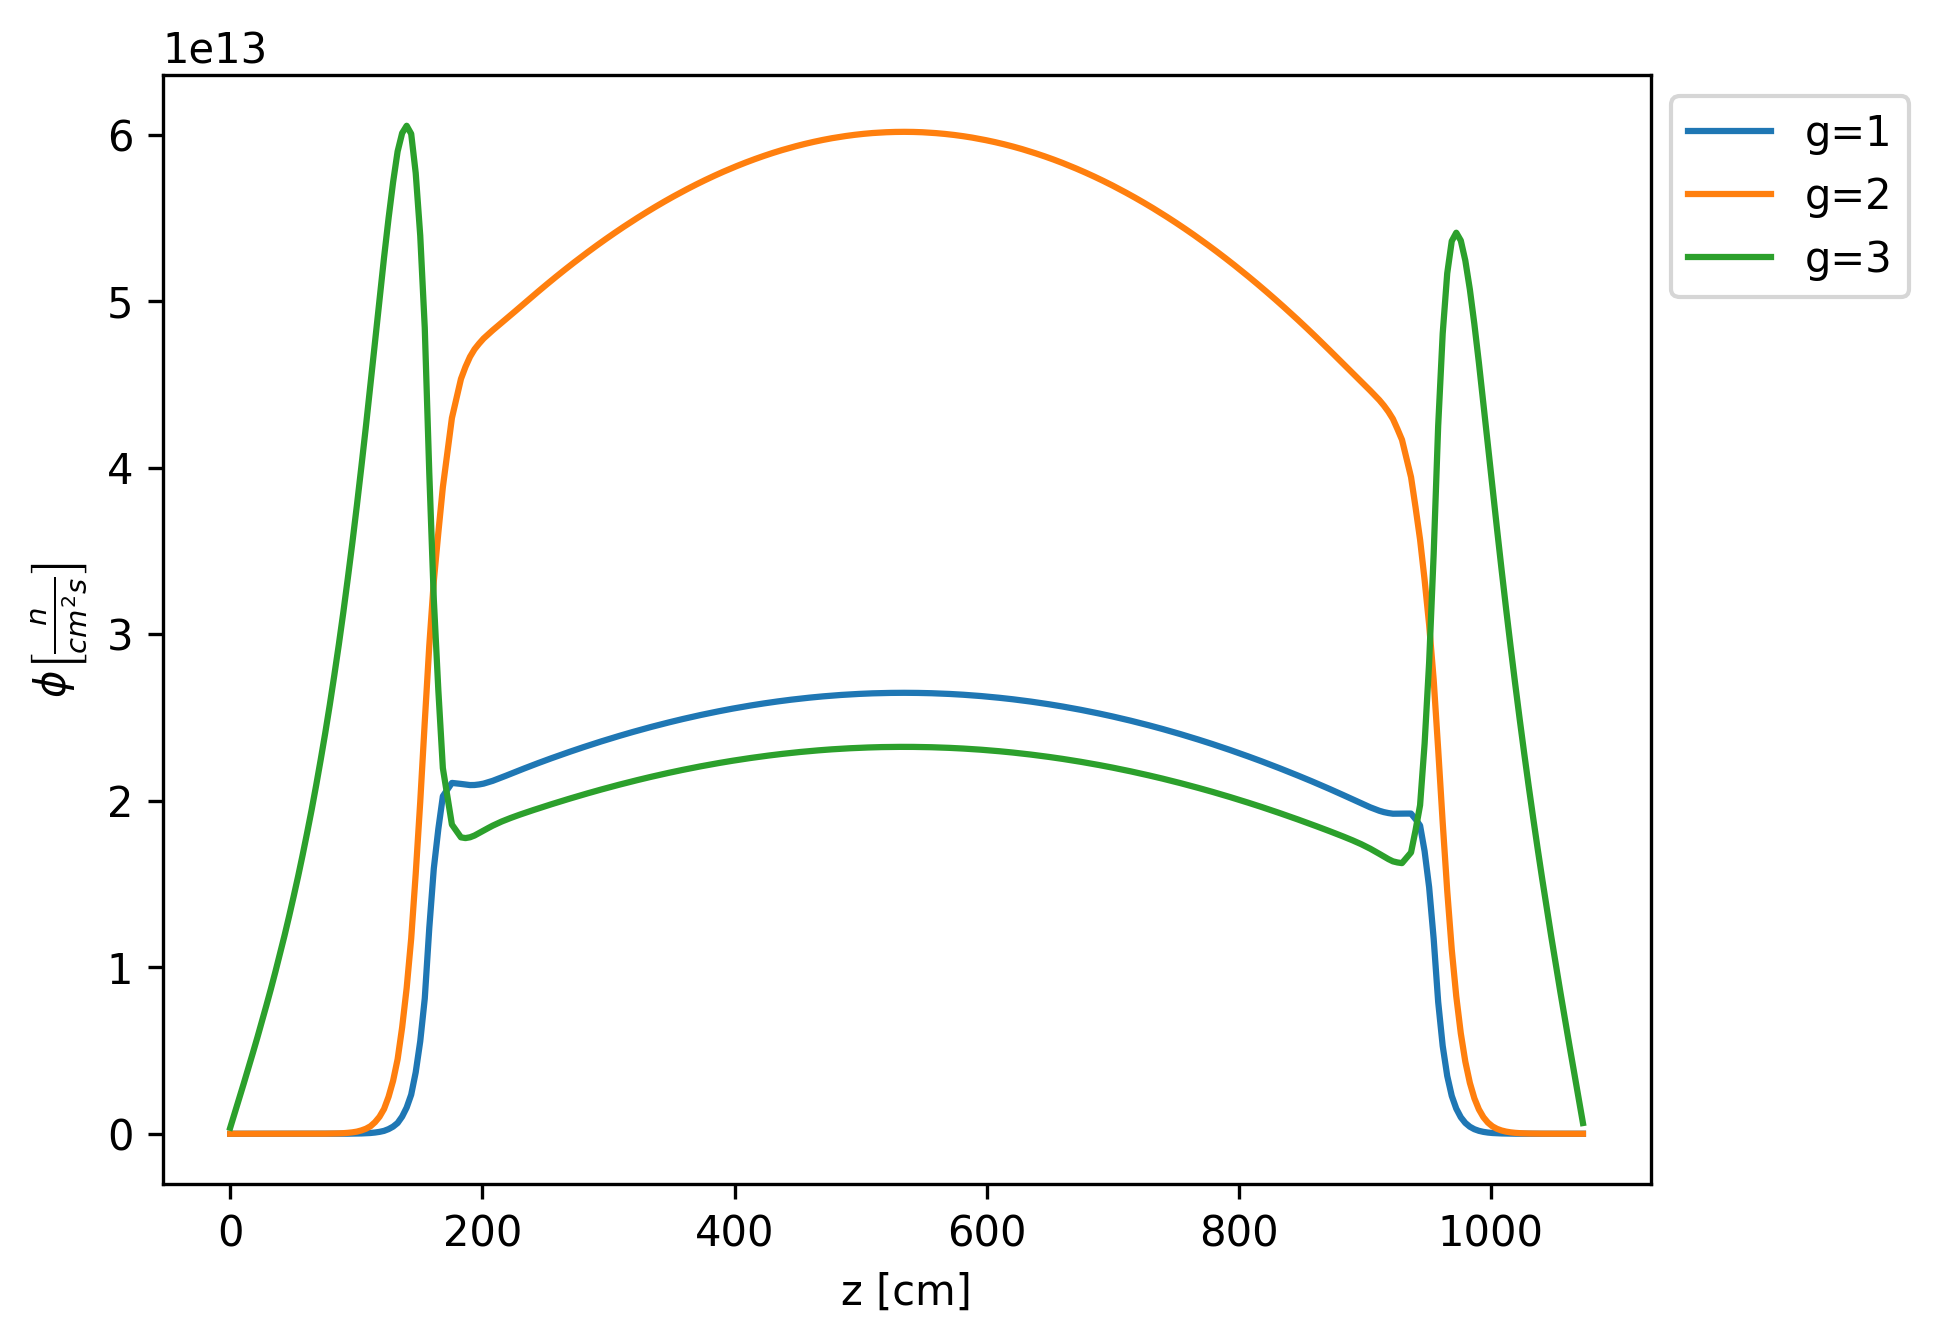
\includegraphics[width=0.45\textwidth]{figures-neutronics/3D-assembly-noLBP-600-26G}
    }
	\hfill
  \caption{Operational case 1: fuel column with no burnable poisons at 600K. Comparison of Serpent and Moltres-derived 3-group axial neutron fluxes.}
	\label{fig:assembly-noLBP-600-flux}
\end{figure}

% No LBP 1200
\begin{figure}[htbp!]
  \centering
    \subfloat[Serpent neutron flux.]{
        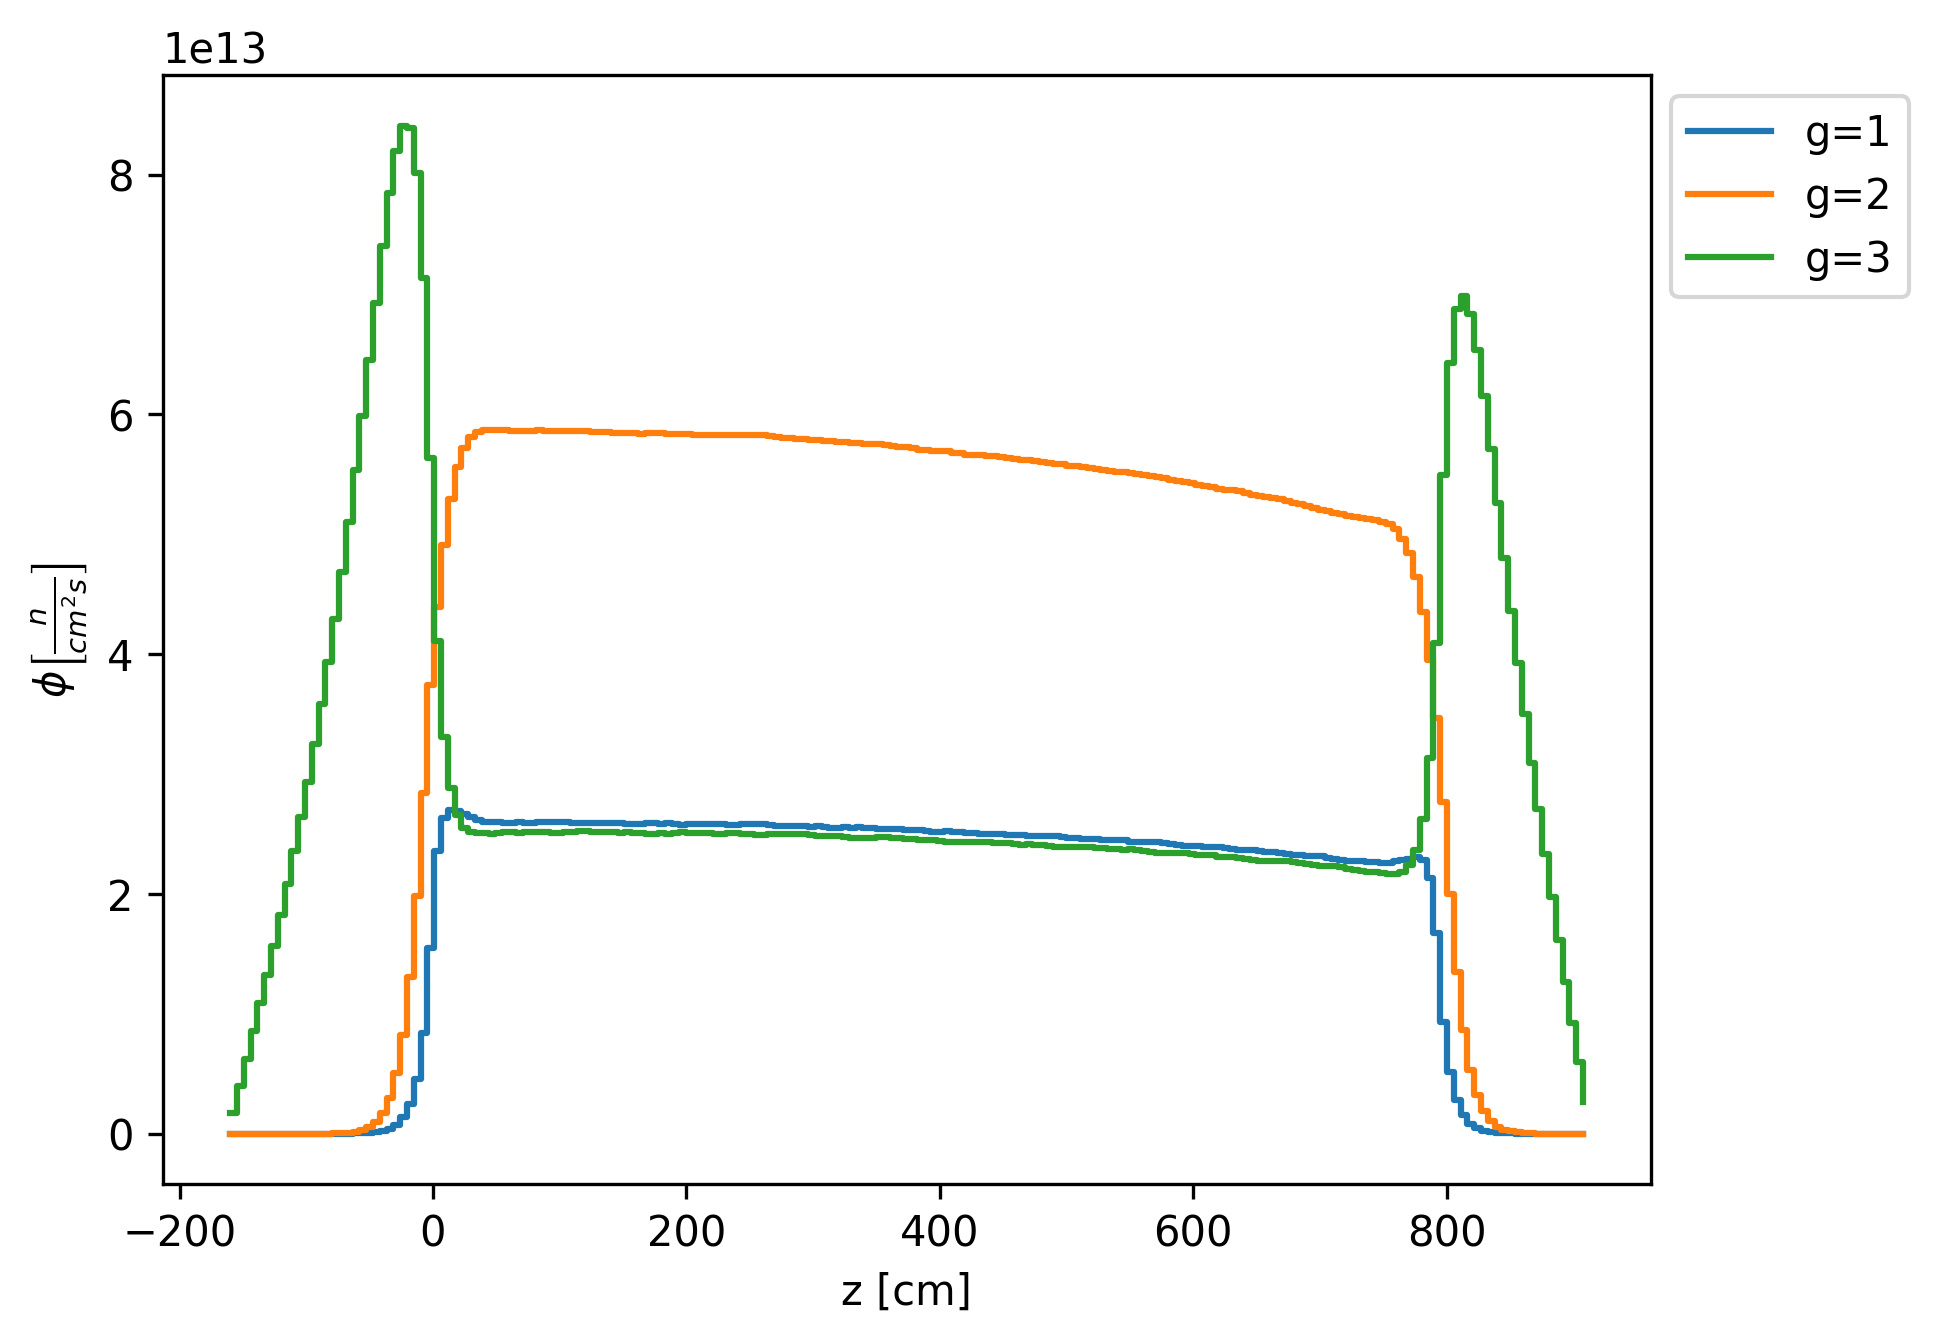
\includegraphics[width=0.45\textwidth]{figures-neutronics/serpent26G-noLBP-1200-collapse}
    }
    \subfloat[Moltres neutron flux.]{
        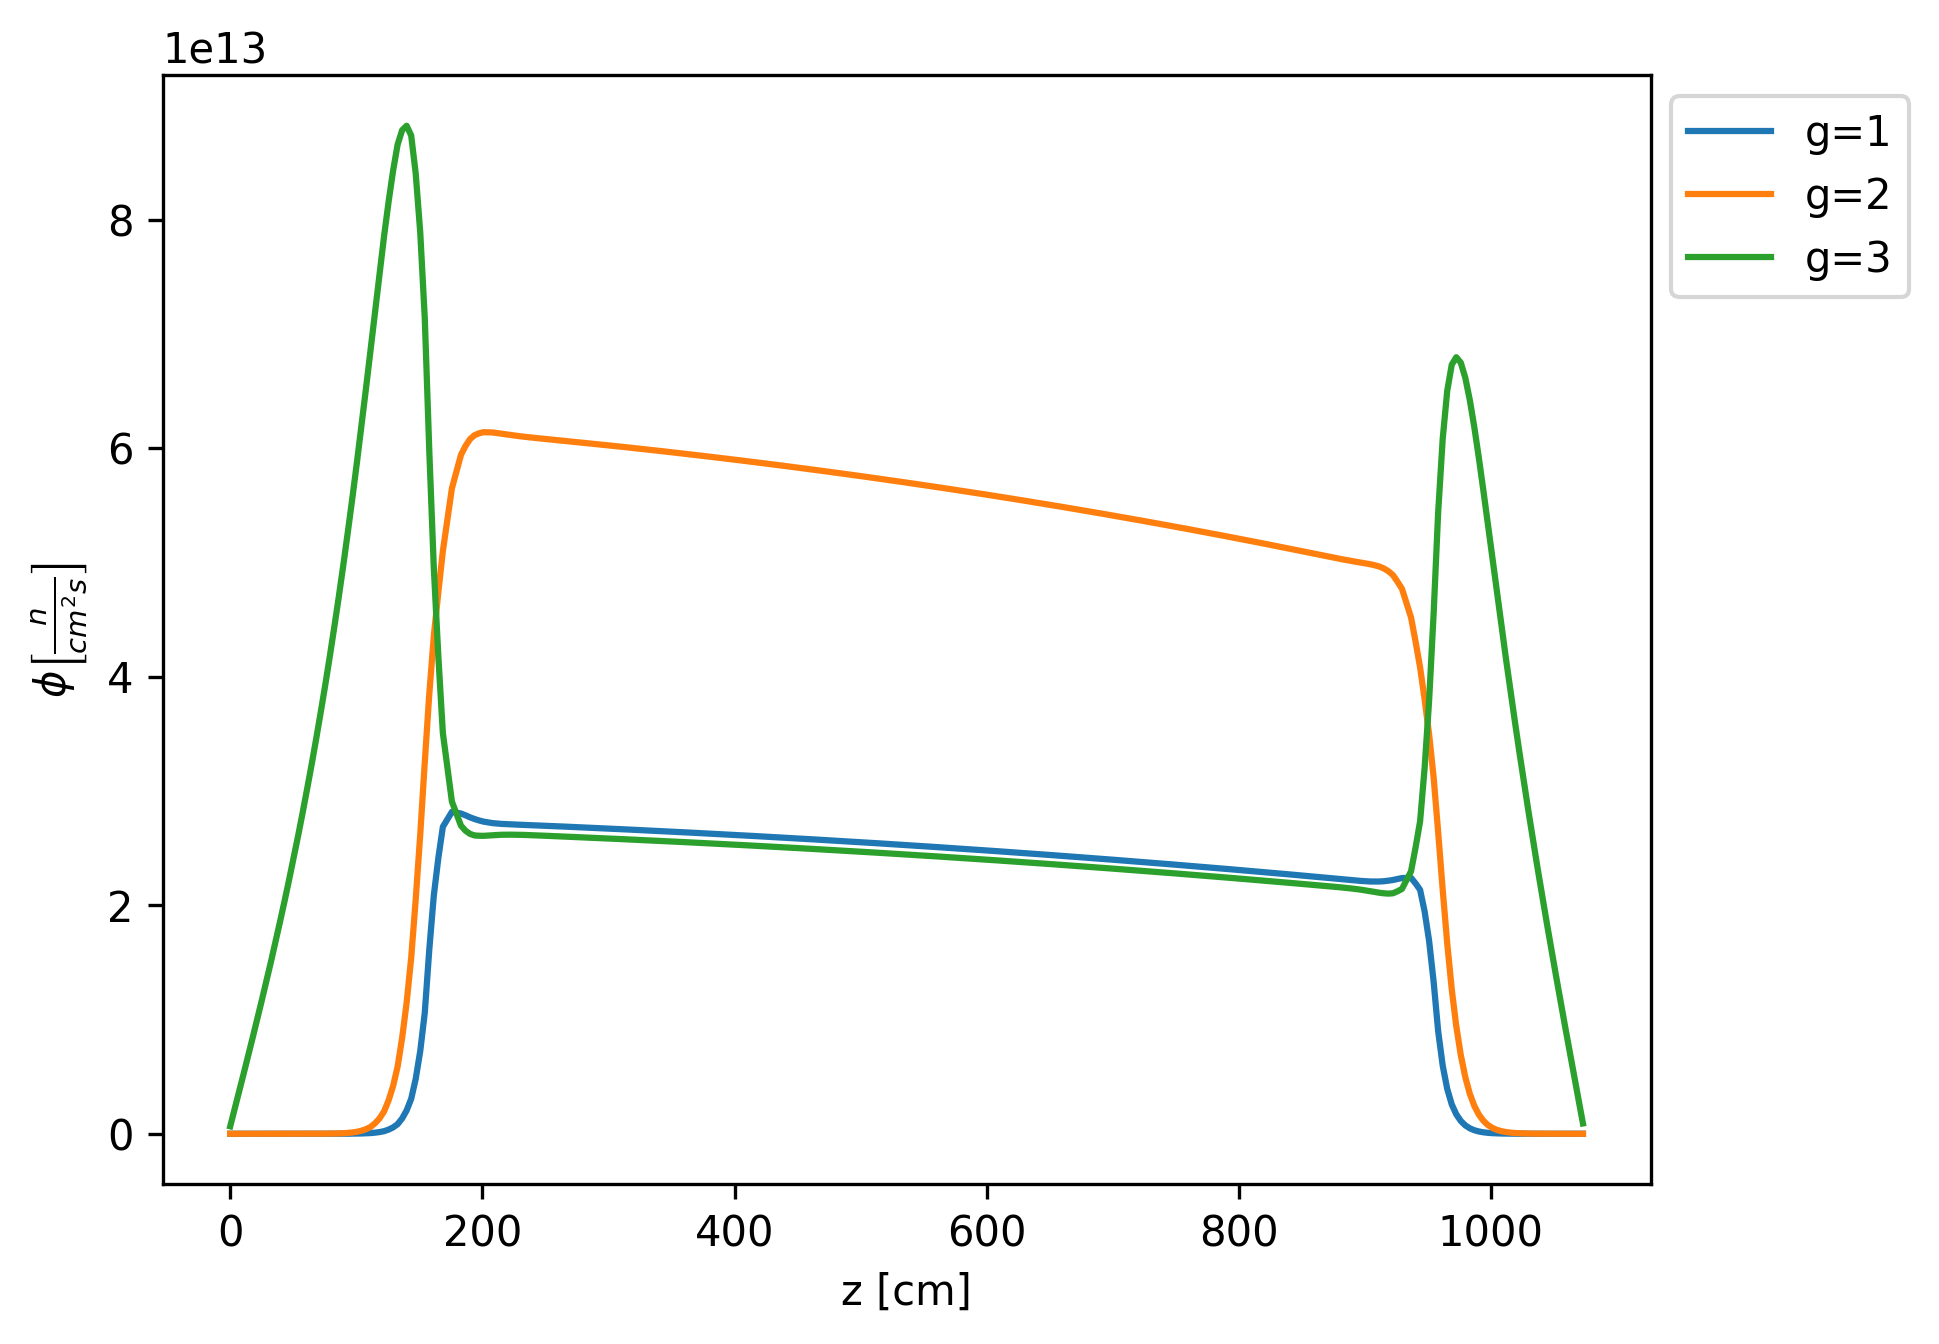
\includegraphics[width=0.45\textwidth]{figures-neutronics/3D-assembly-noLBP-1200-26G}
    }
  \hfill
  \caption{Operational case 2: fuel column with no burnable poisons at 1200K. Comparison of Serpent and Moltres-derived 3-group axial neutron fluxes.}
  \label{fig:assembly-noLBP-1200-flux}
\end{figure}

% LBP 600 
\begin{figure}[htbp!]
  \centering
    \subfloat[Serpent neutron flux.]{
        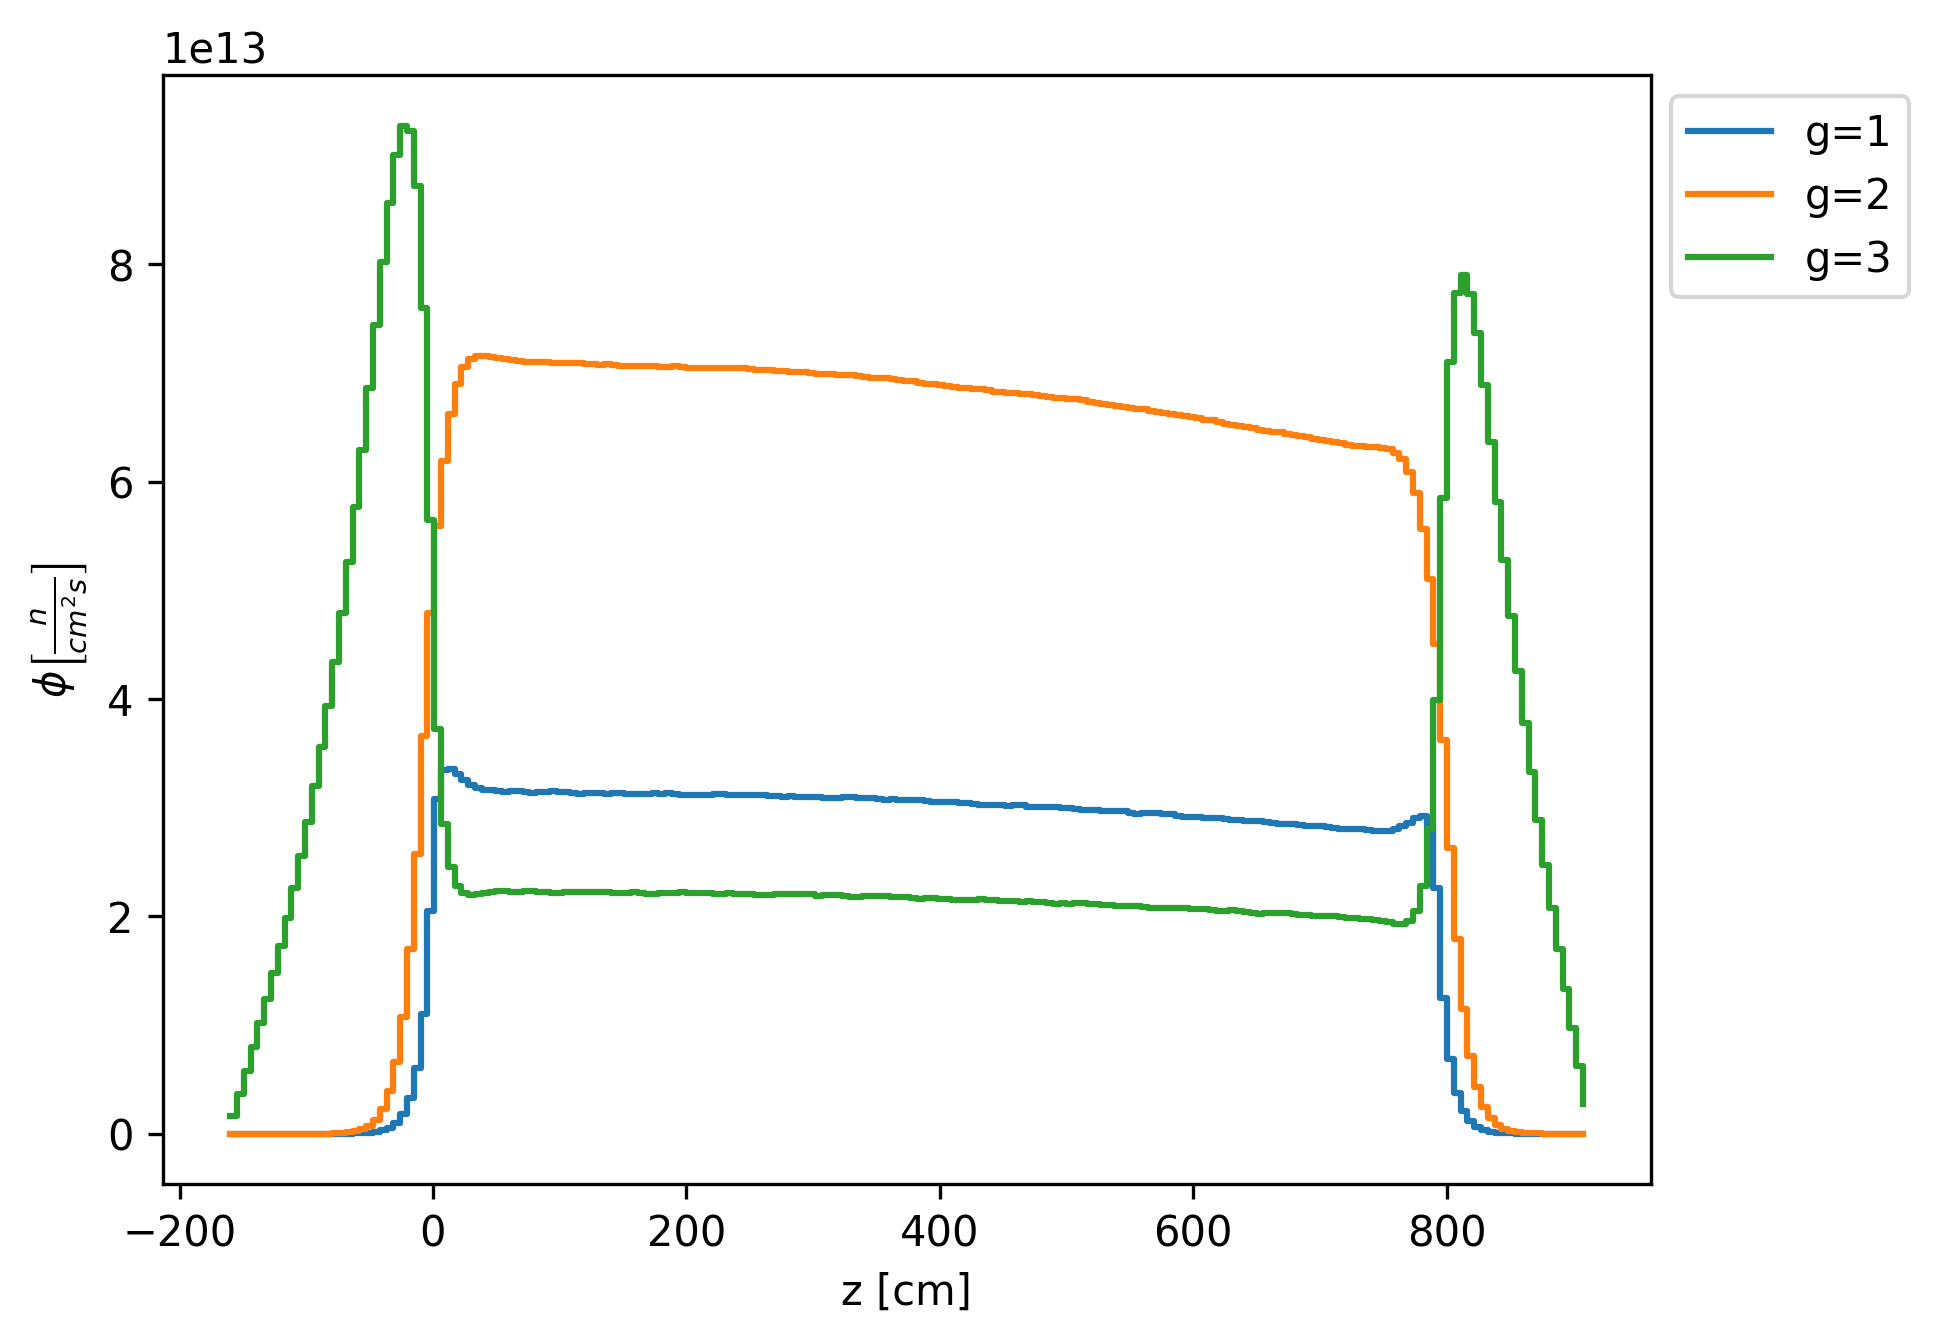
\includegraphics[width=0.45\textwidth]{figures-neutronics/serpent26G-LBP-600-collapse}
    }
    \subfloat[Moltres neutron flux.]{
        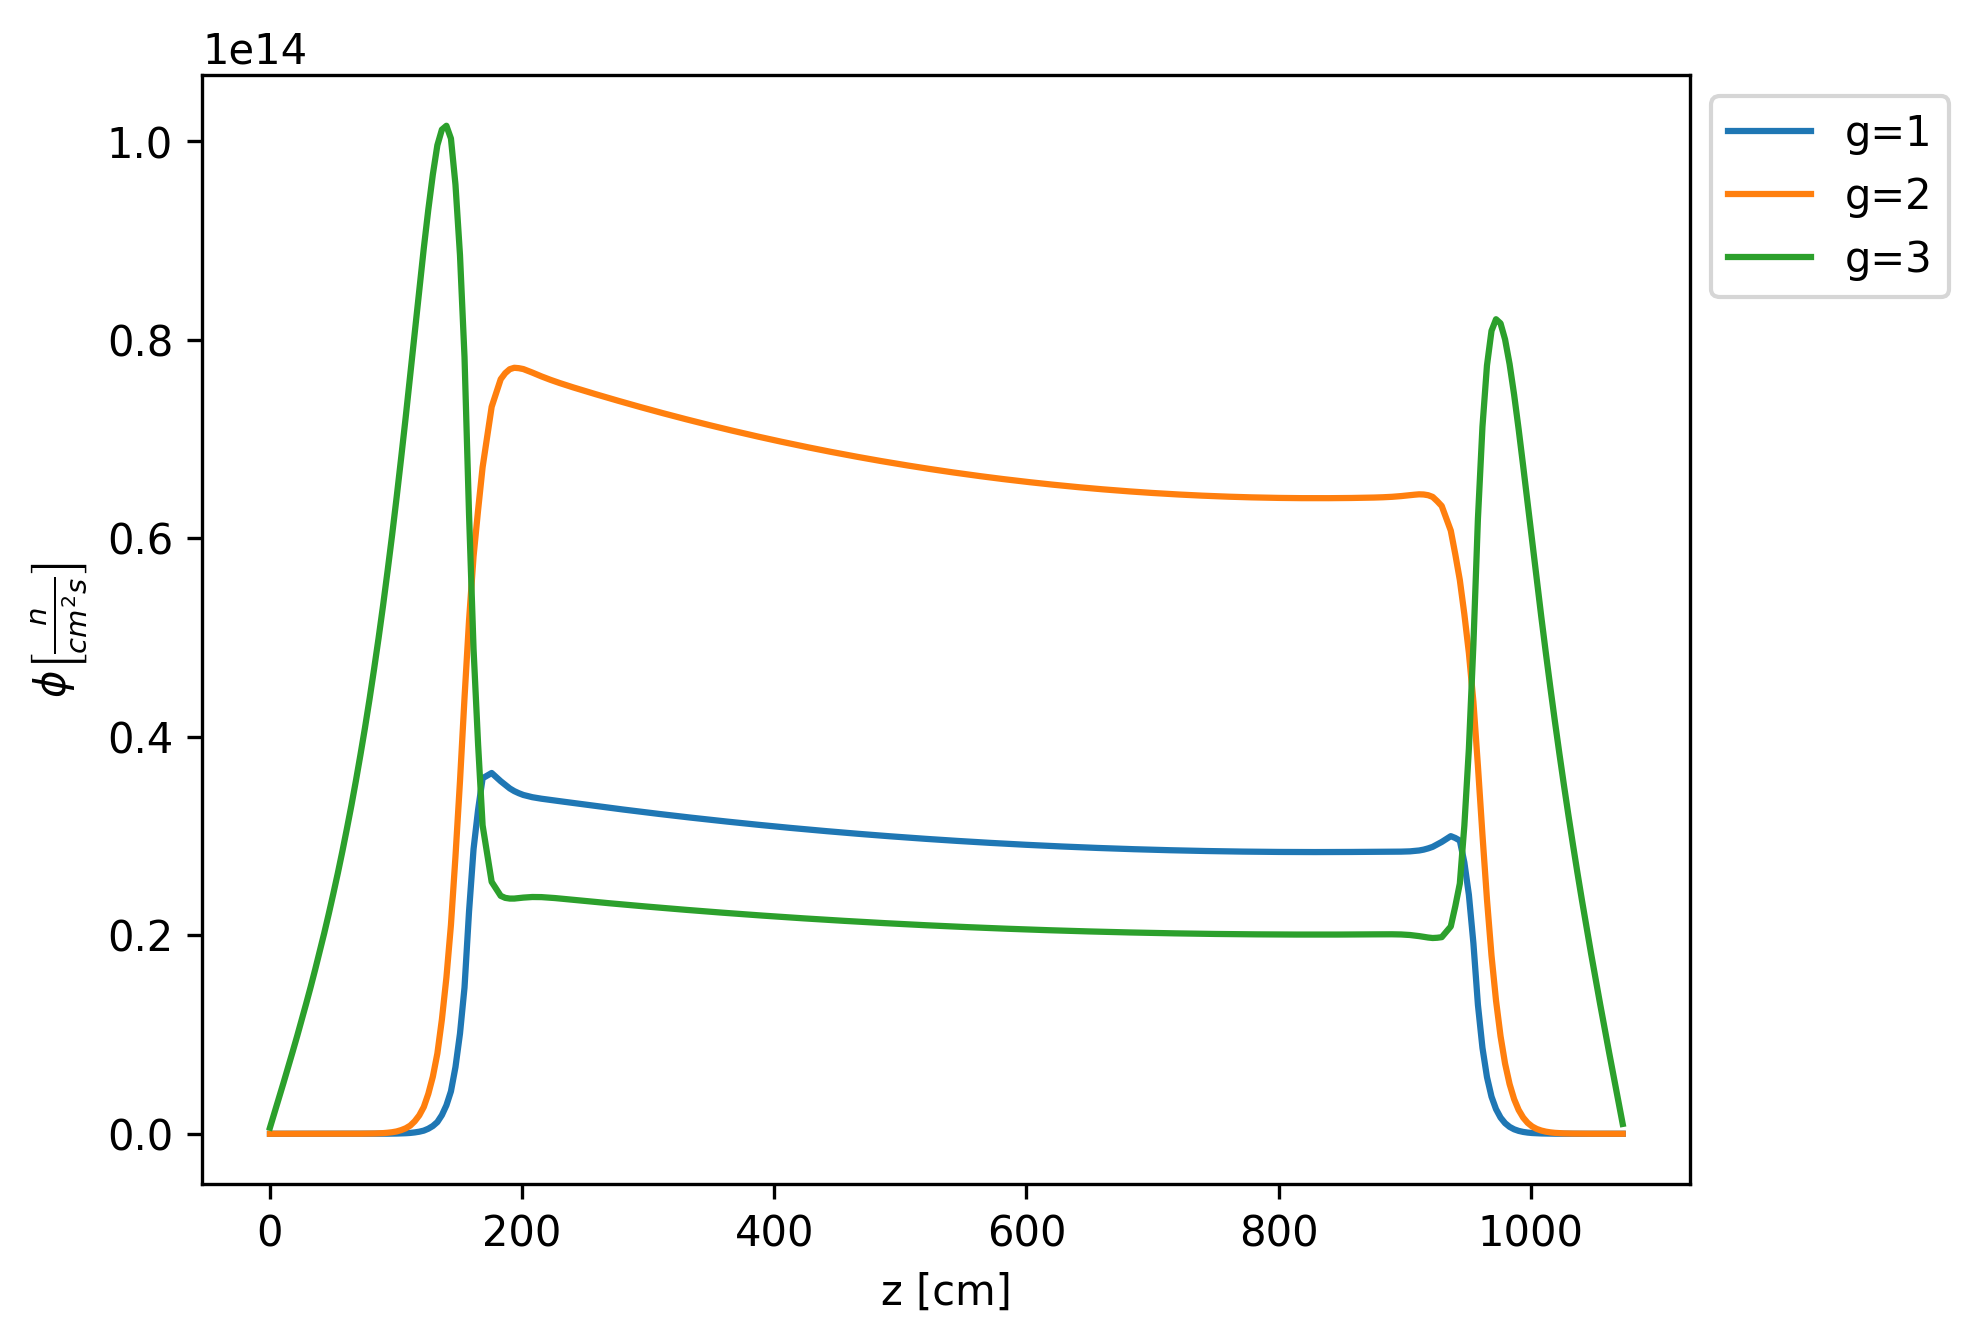
\includegraphics[width=0.45\textwidth]{figures-neutronics/3D-assembly-LBP-600-26G}
    }
  \hfill
  \caption{Operational case 3: fuel column with burnable poisons at 600K. Comparison of Serpent and Moltres-derived 3-group axial neutron fluxes.}
  \label{fig:assembly-LBP-600-flux}
\end{figure}

% LBP 1200
\begin{figure}[htbp!]
  \centering
    \subfloat[Serpent neutron flux.]{
        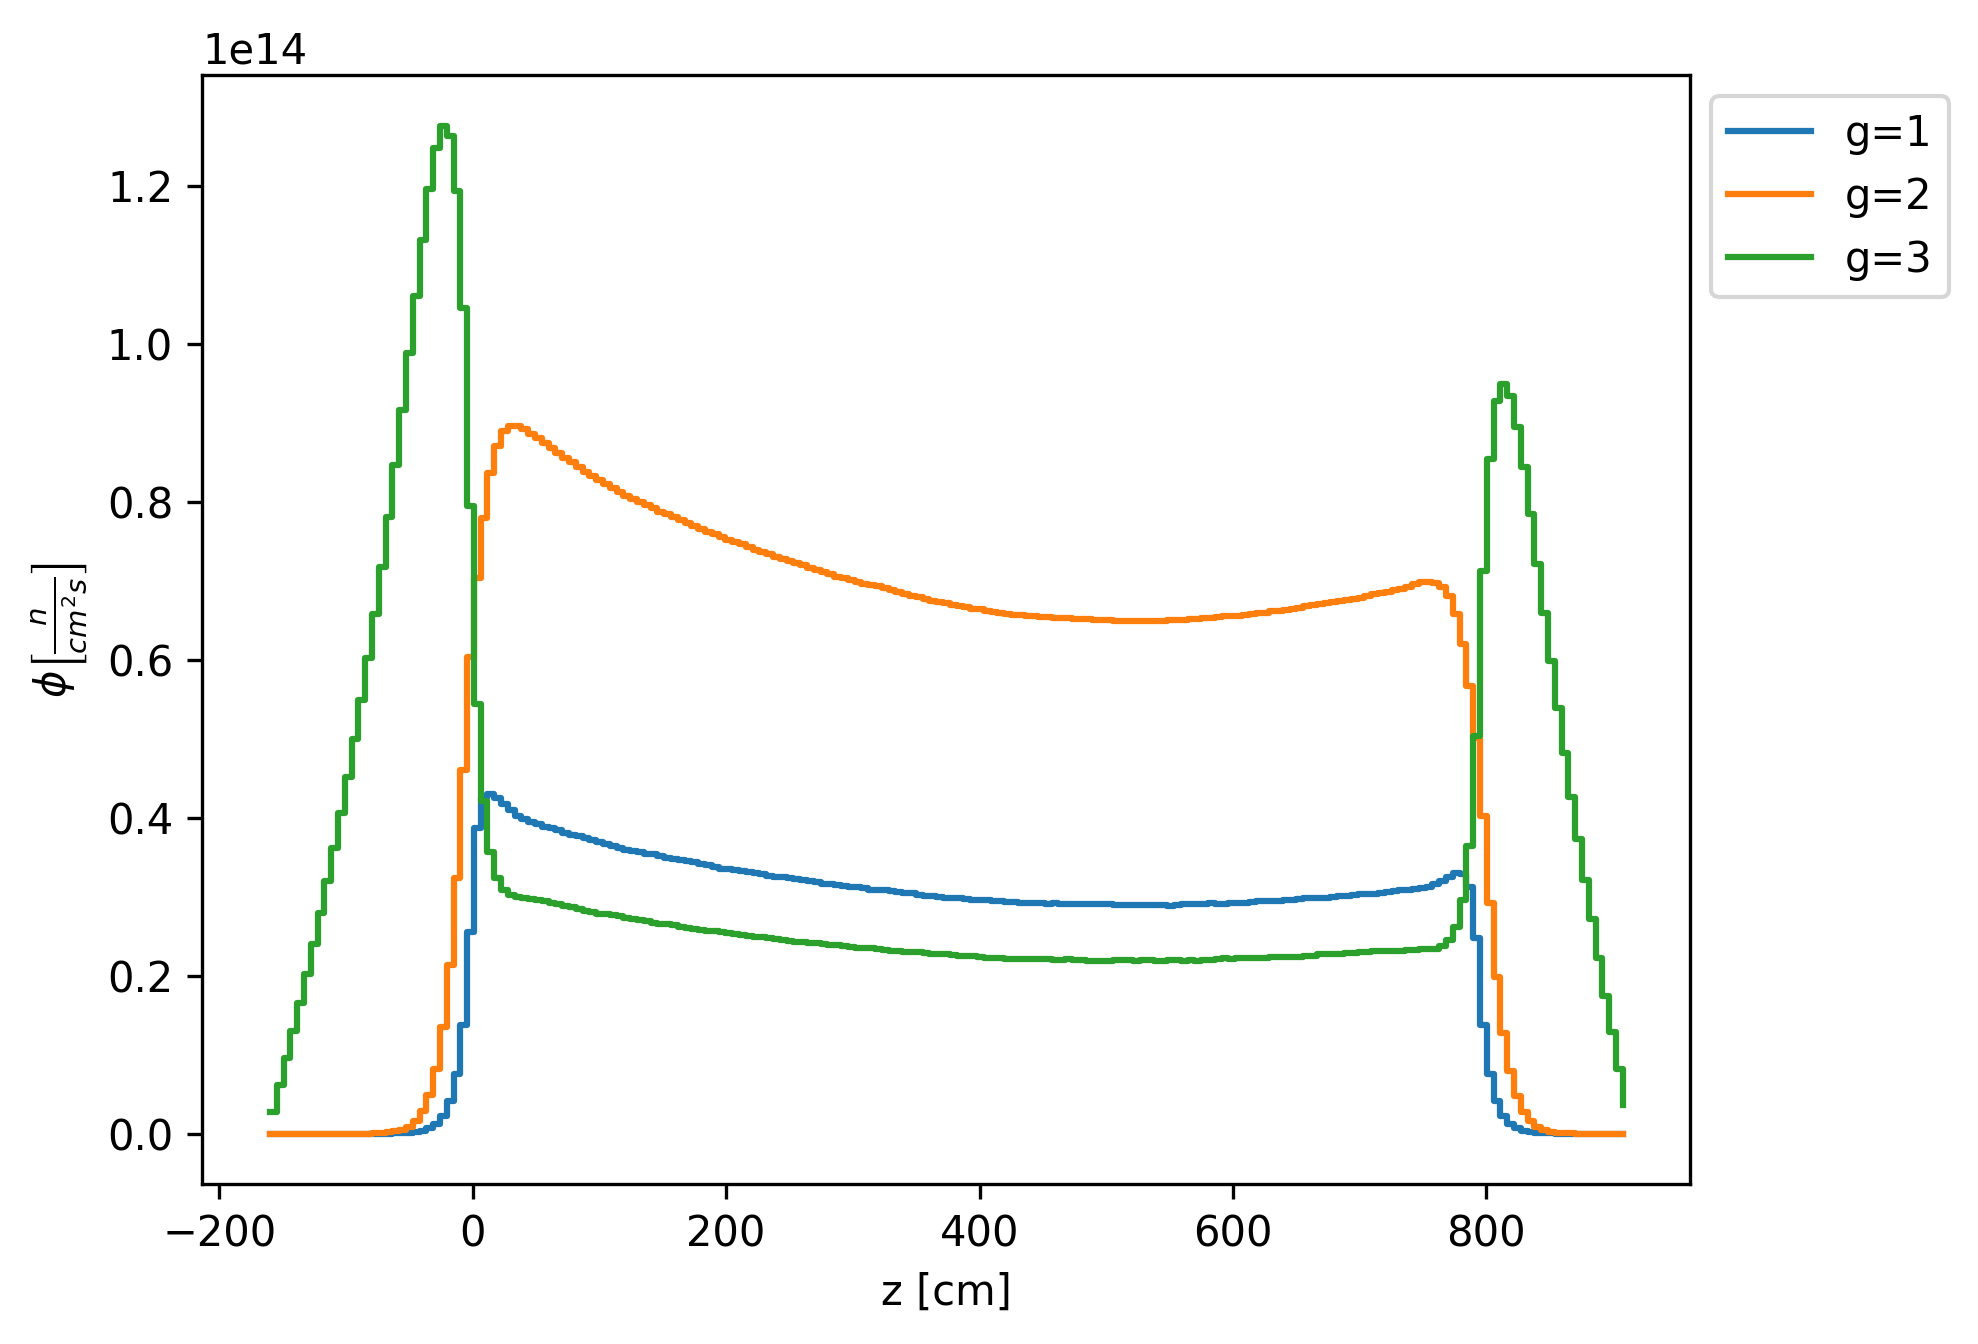
\includegraphics[width=0.45\textwidth]{figures-neutronics/serpent26G-LBP-1200-collapse}
    }
    \subfloat[Moltres neutron flux.]{
        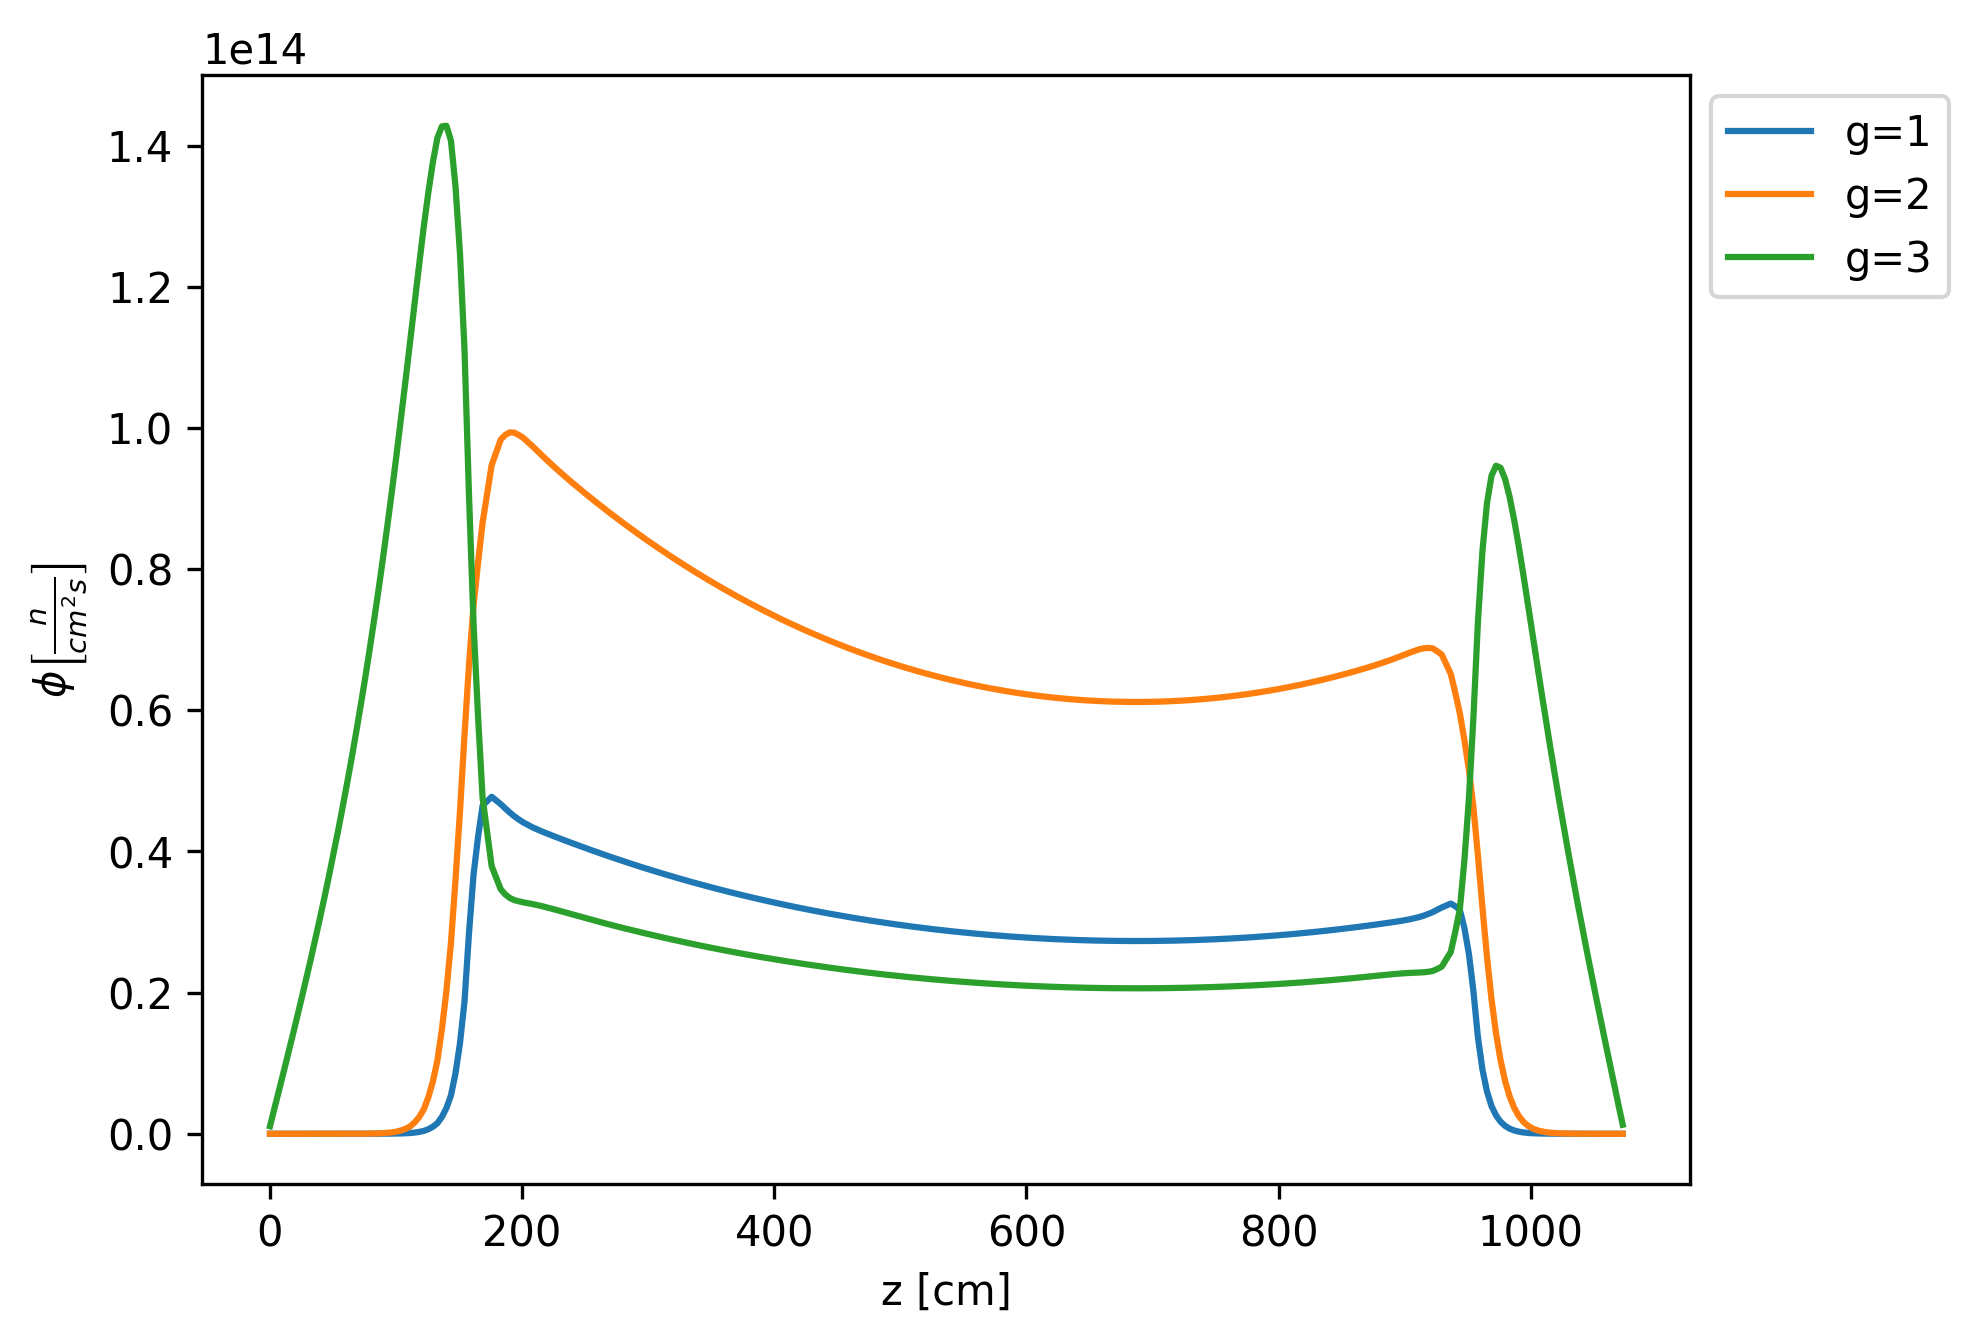
\includegraphics[width=0.45\textwidth]{figures-neutronics/3D-assembly-LBP-1200-26G}
    }
  \hfill
  \caption{Operational case 4: fuel column with burnable poisons at 1200K. Comparison of Serpent and Moltres-derived 3-group axial neutron fluxes.}
  \label{fig:assembly-LBP-1200-flux}
\end{figure}

% eigenvalues
Equation \ref{eq:delta-rho} calculates the reactivity difference ($\Delta \rho$) between the eigenvalues calculated by Serpent and Moltres
\begin{align}
	& \Delta \rho = \left| \rho_1 - \rho_2 \right| = \left| \frac{k_1-1}{k_1} - \frac{k_2-1}{k_2} \right| = \left| \frac{k_1-k_2}{k_1 k_2} \right| \label{eq:delta-rho} \\
  \intertext{where}
  & k_1 = \mbox{Serpent-derived eigenvalue} [-] \notag \\
  & k_2 = \mbox{Moltres-derived eigenvalue} [-]. \notag
\end{align}

Table \ref{tab:keff} exhibits the eigenvalues calculated by Serpent and $\Delta \rho$ for the different energy group structures.
The eigenvalues in Moltres differ slightly from the eigenvalues in Serpent, and overall, the reactivity difference is less than 50 pcm.
The number of energy groups does not affect the accuracy of the eigenvalue calculations in Moltres.

\begin{table}[htbp!]
  \centering
  \caption{Eigenvalues calculated by Serpent and reactivity difference between eigenvalues calculated by Moltres and Serpent, see equation \ref{eq:delta-rho}, for the different energy group structures.}
  \begin{tabular}{c|c|cccccccc}
  \toprule
Operational case  & Serpent       & \multicolumn{8}{c}{$\Delta \rho$ [pcm]}            \\ \cline{3-10} 
                  & eigenvalues   & 3   & 6   & 9   & 12   & 15   & 18   & 21   & 26   \\
  \midrule
1 & 1.43800 $\pm$ 0.00008 & 10  & 7   & 6   & 6    & 5    & 6    & 6    & 12   \\
2 & 1.37771 $\pm$ 0.00008 & 23  & 15  & 4   & 3    & 2    & 2    & 1    & 11   \\
3 & 1.12861 $\pm$ 0.00009 & 44  & 21  & 24  & 25   & 25   & 24   & 19   & 9    \\
4 & 1.06554 $\pm$ 0.00010 & 36  & 40  & 29  & 32   & 44   & 43   & 25   & 25   \\
  \bottomrule
  \end{tabular}
  \label{tab:keff}
\end{table}

The last analysis is for the Moltres axial flux.
Considering the 26 group structure as the reference value, equation \ref{eq:l2norm} obtained the $L_2$-norm of the active core's axial flux relative difference
\begin{align}
  & \Delta_{L_2} = \left\| \frac{\phi_G(z)-\phi_{ref}(z)}{\phi_{ref}(z)} \right\|  \quad \wedge \quad z\quad \in \quad L_a \label{eq:l2norm}
  \intertext{where}
  & \Delta_{L_2} = \mbox{L$_2$-norm relative difference } [-] \notag \\
  & \phi_G(z) = \mbox{$G$-energy groups axial flux } [n \cdot cm^{-2} \cdot s^{-1}] \notag \\
  & \phi_{ref}(z) = \mbox{reference axial flux } [n \cdot cm^{-2} \cdot s^{-1}] \notag \\
  & L_a = \mbox{active core length } [cm]. \notag
\end{align}

Figures \ref{fig:assembly-noLBP-er} and \ref{fig:assembly-LBP-er} show $\Delta_{L_2}$ for the various energy group structures.
Overall, the relative error decreases with an increase in the number of energy groups.
Nonetheless, this is not always the case.
For example, in Figure \ref{fig:assembly-noLBP-er-b}, from 12 to 15-energy groups, the thermal flux agreement improves, but the fast flux agreement worsens.
Additionally, the relative error of the cases with no burnable poisons is smaller than the relative error of the cases with burnable poison.
The treatment of the burnable poisons challenges the accuracy of the homogenized simulations in Moltres.
For example, a three-energy group structure yields more than 100$\%$ error when treating the burnable poison, Figure \ref{fig:assembly-LBP-er}.

% No LBP
\begin{figure}[htbp!]
	\centering
    \subfloat[Operational case 1: 600K.]{
        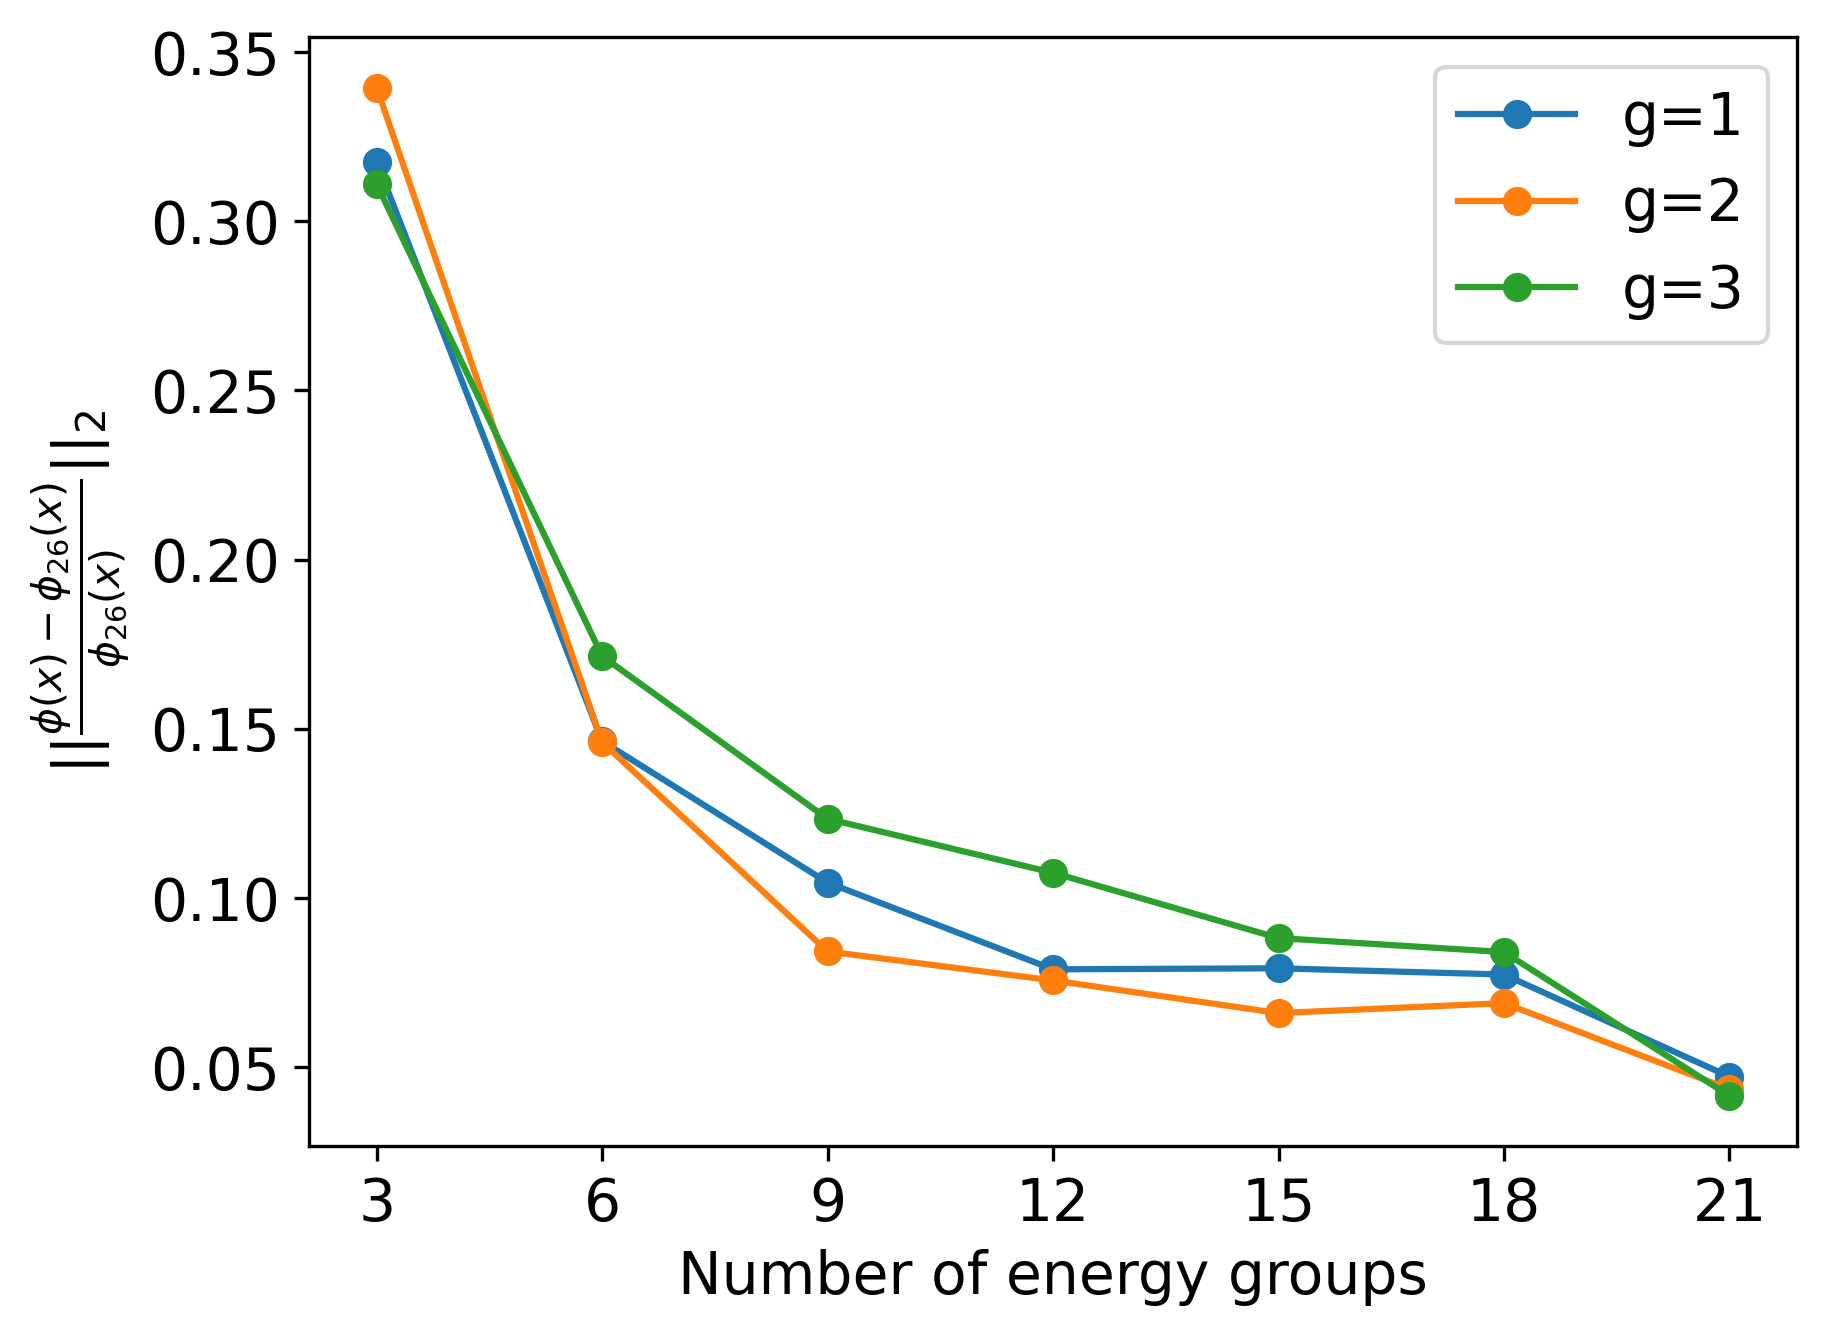
\includegraphics[width=0.45\textwidth]{figures-neutronics/noLBP-600-er-final}
    }
    \subfloat[Operational case 2: 1200K.\label{fig:assembly-noLBP-er-b}]{
        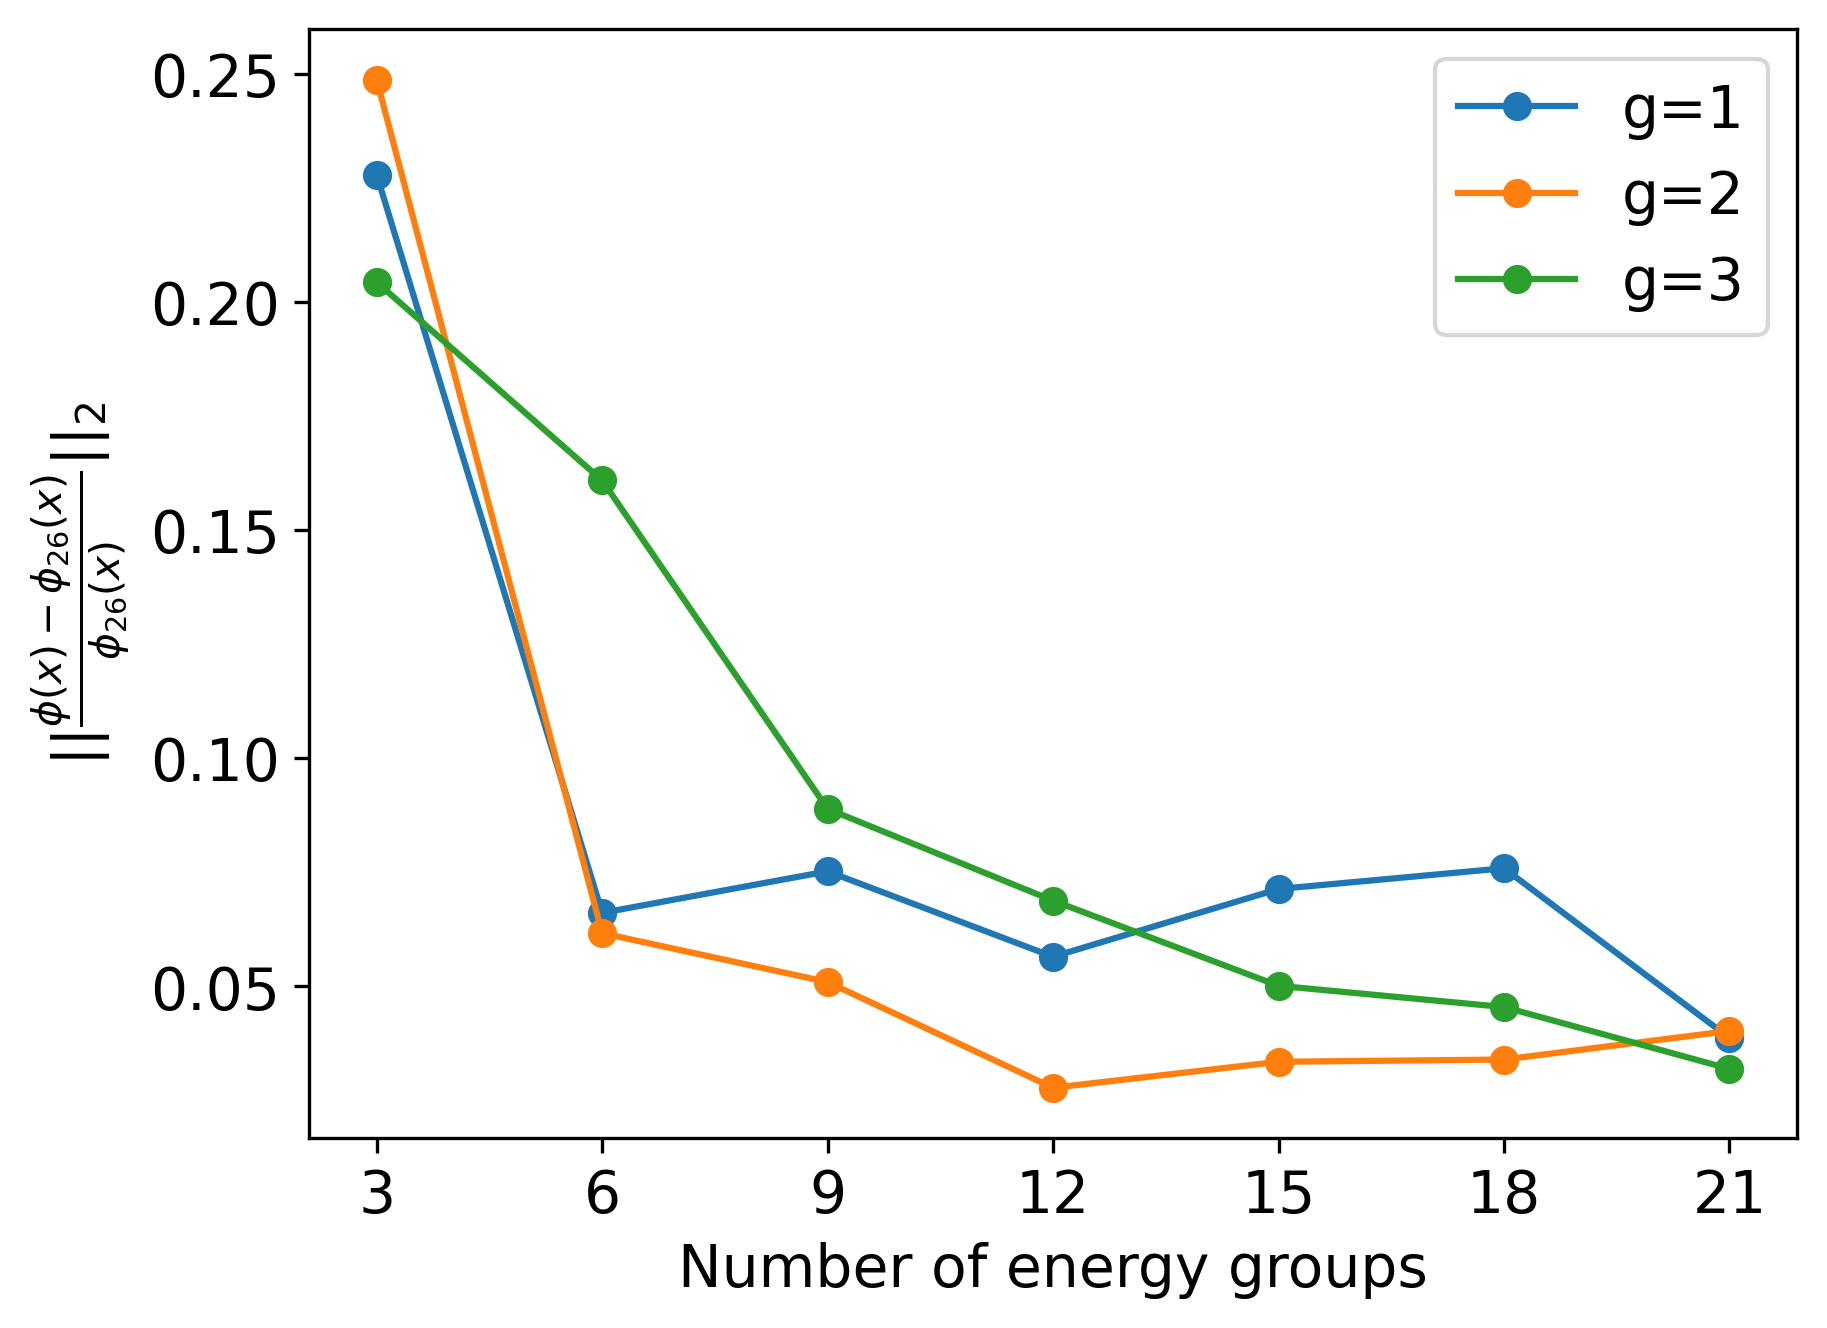
\includegraphics[width=0.45\textwidth]{figures-neutronics/noLBP-1200-er-final}
    }
	\hfill
    \caption{L$_2$-norm relative error for different number of energy group structures for the operational cases with no burnable poisons.}
	\label{fig:assembly-noLBP-er}
\end{figure}

% LBP
\begin{figure}[htbp!]
	\centering
    \subfloat[Operational case 3: 600K.]{
        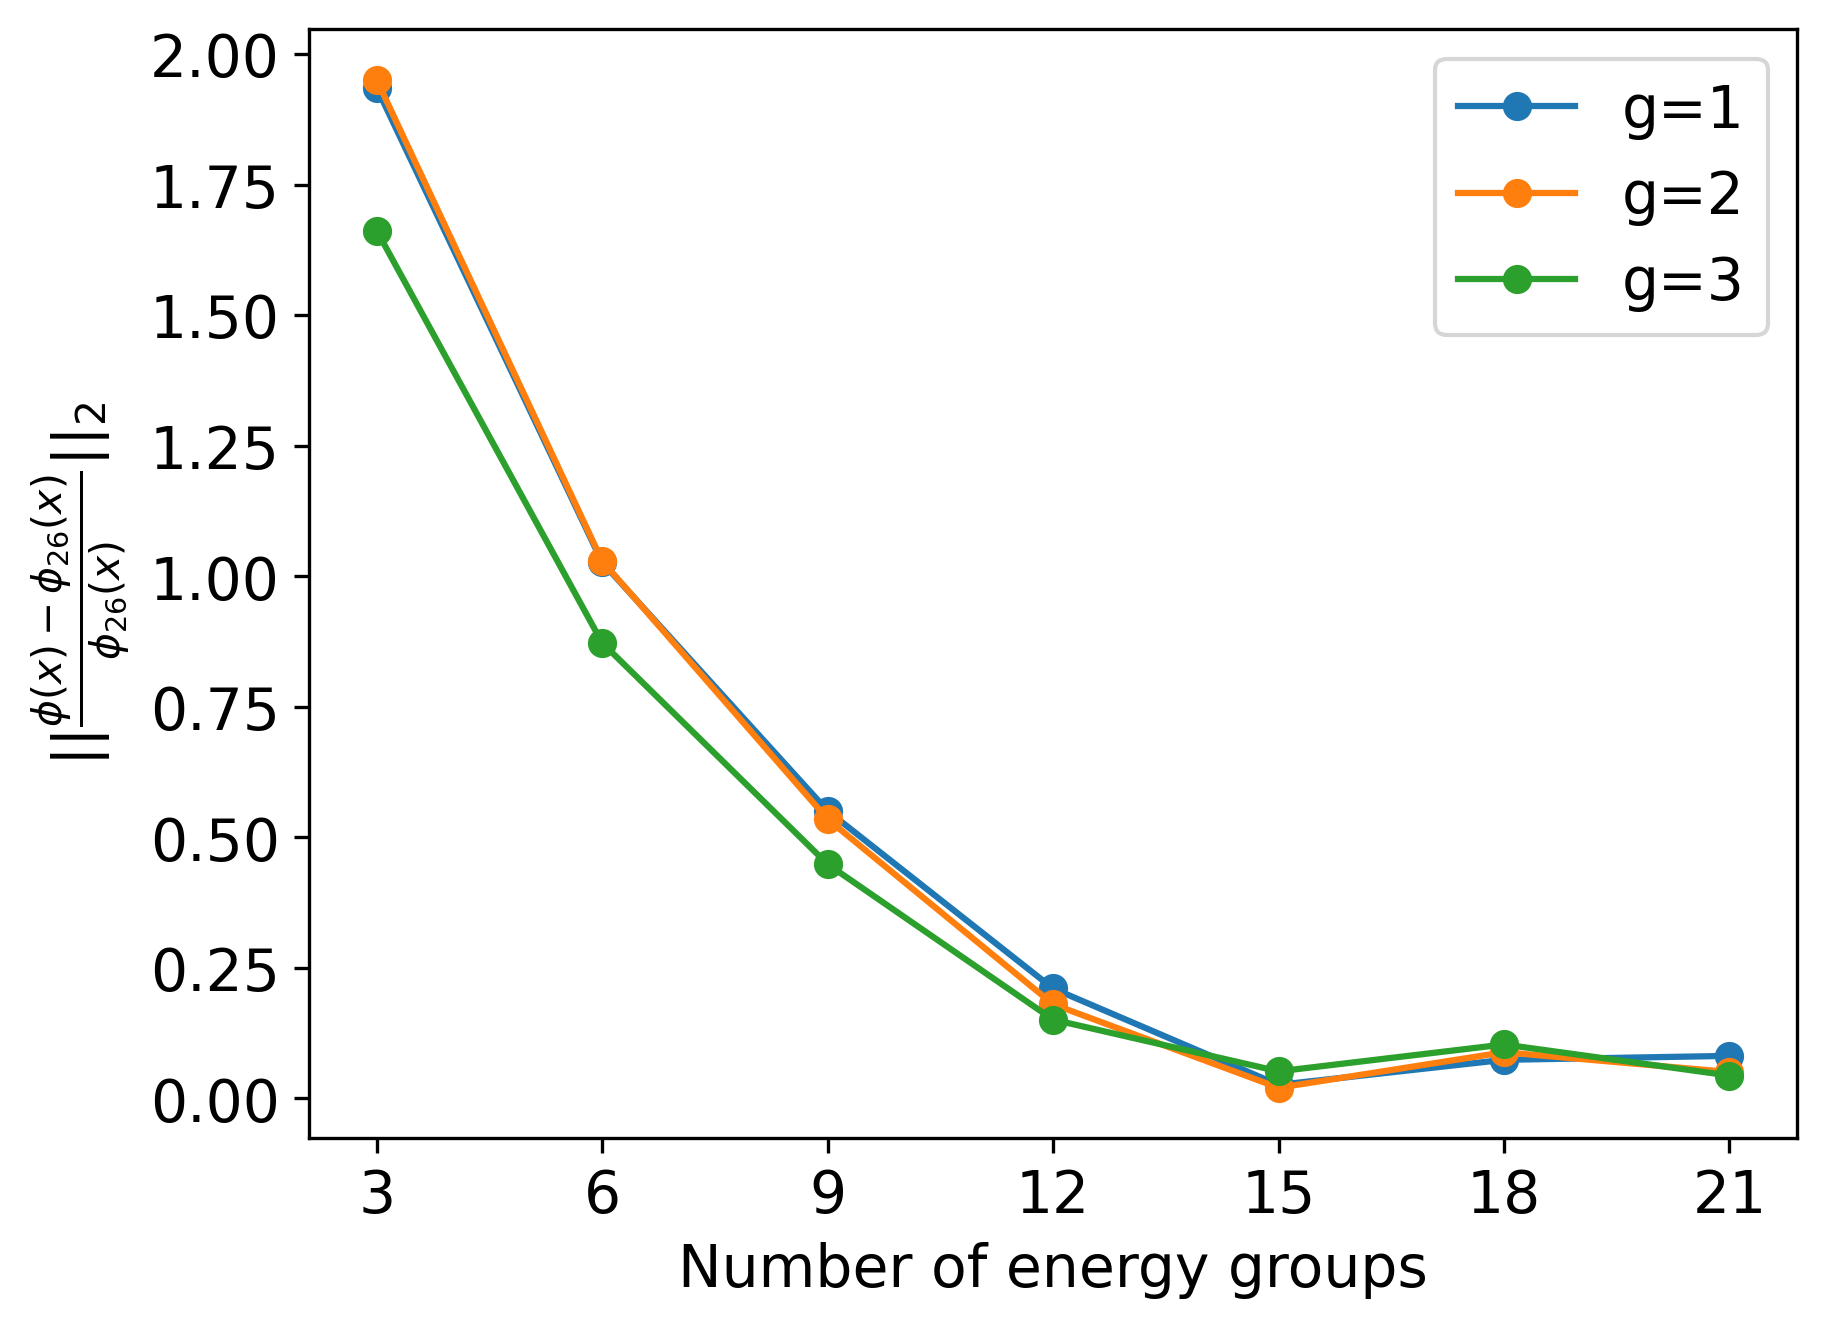
\includegraphics[width=0.45\textwidth]{figures-neutronics/LBP-600-er-final}
    }
    \subfloat[Operational case 4: 1200K.]{
        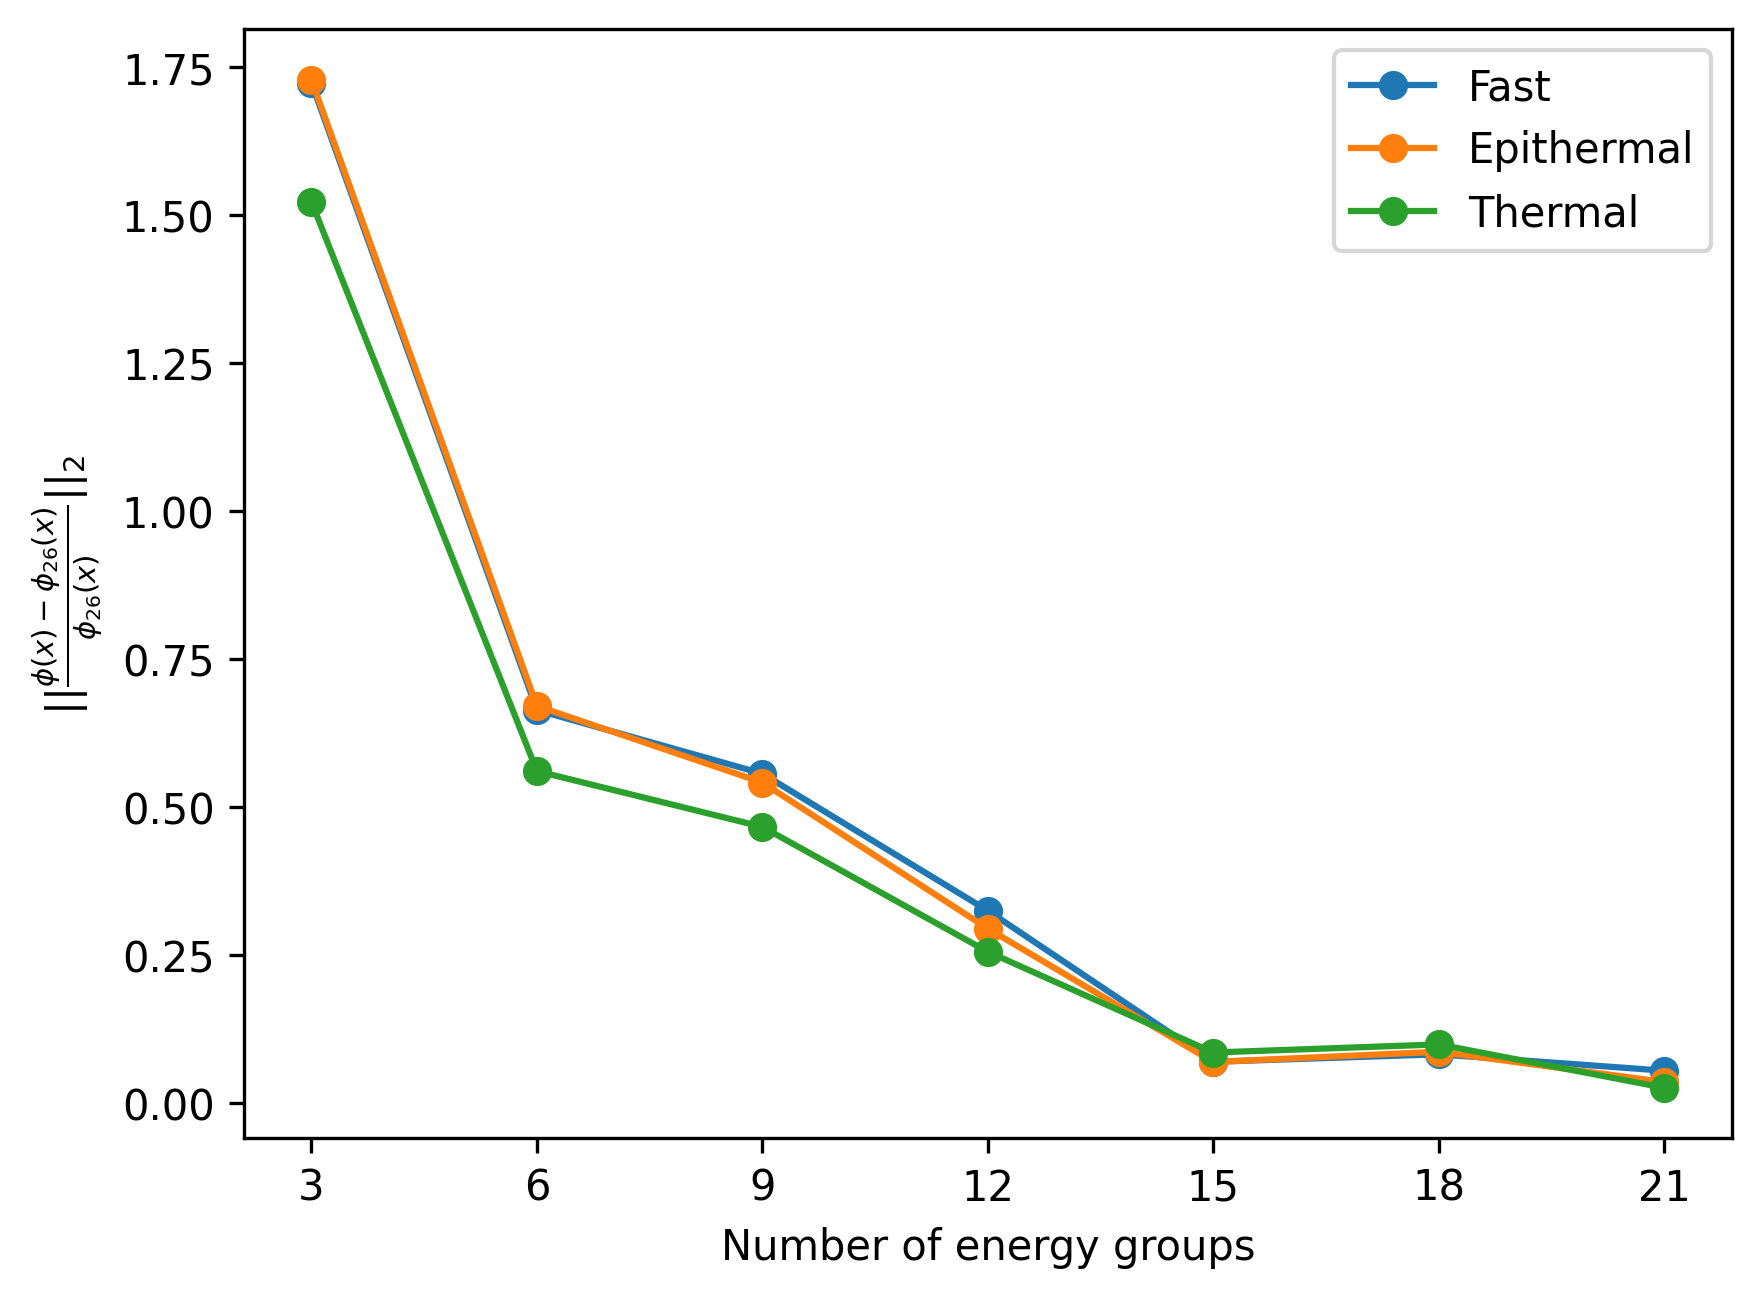
\includegraphics[width=0.45\textwidth]{figures-neutronics/LBP-1200-er-final}
    }
	\hfill
    \caption{LBP case. L$_2$-norm relative error for different number of energy group structures for the operational cases with burnable poisons.}
	\label{fig:assembly-LBP-er}
\end{figure}

The analysis also included the computational time and the peak memory usage during the simulations, as shown in Figure \ref{fig:assembly-time}.
All the simulations used 128 cores.
This section presents only the cases at 600K because the impact of the temperature change was not significant.
The computational requirements rise with an increase in the number of energy groups.
As the geometry uses a constant number of elements, the number of DoFs per energy-group remains constant for all the simulations.
Figure \ref{fig:assembly-time} also shows that the overall time of the cases with burnable poison is higher than the cases without them.

% Time and memory
\begin{figure}[htbp!]
	\centering
    \subfloat[No burnable poisons at 600 K.]{
        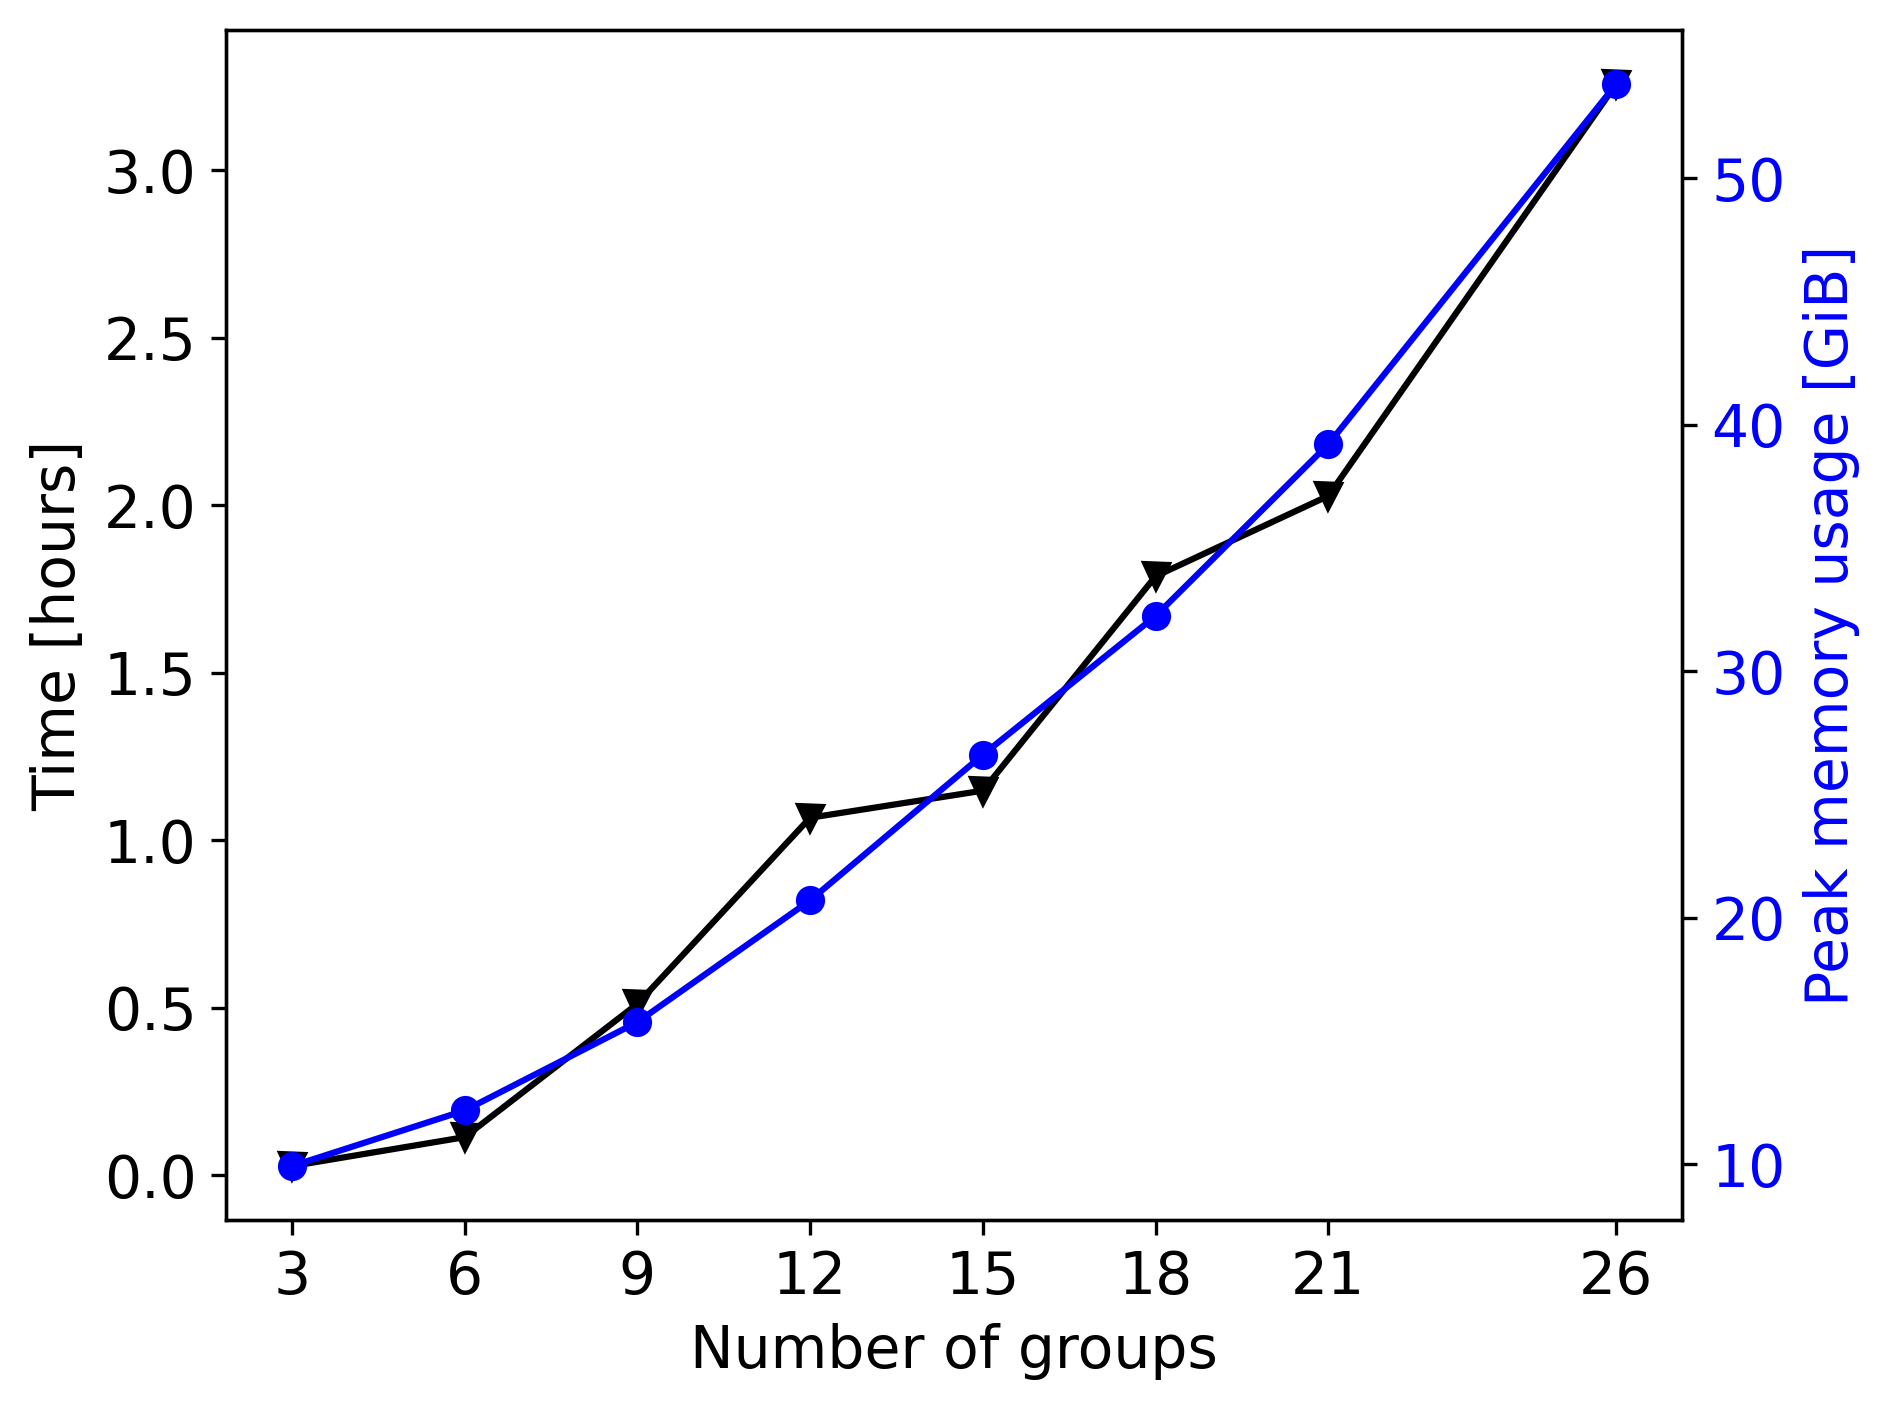
\includegraphics[width=0.45\textwidth]{figures-neutronics/time-noLBP-600}
    }
    \subfloat[Burnable poisons at 600 K.]{
        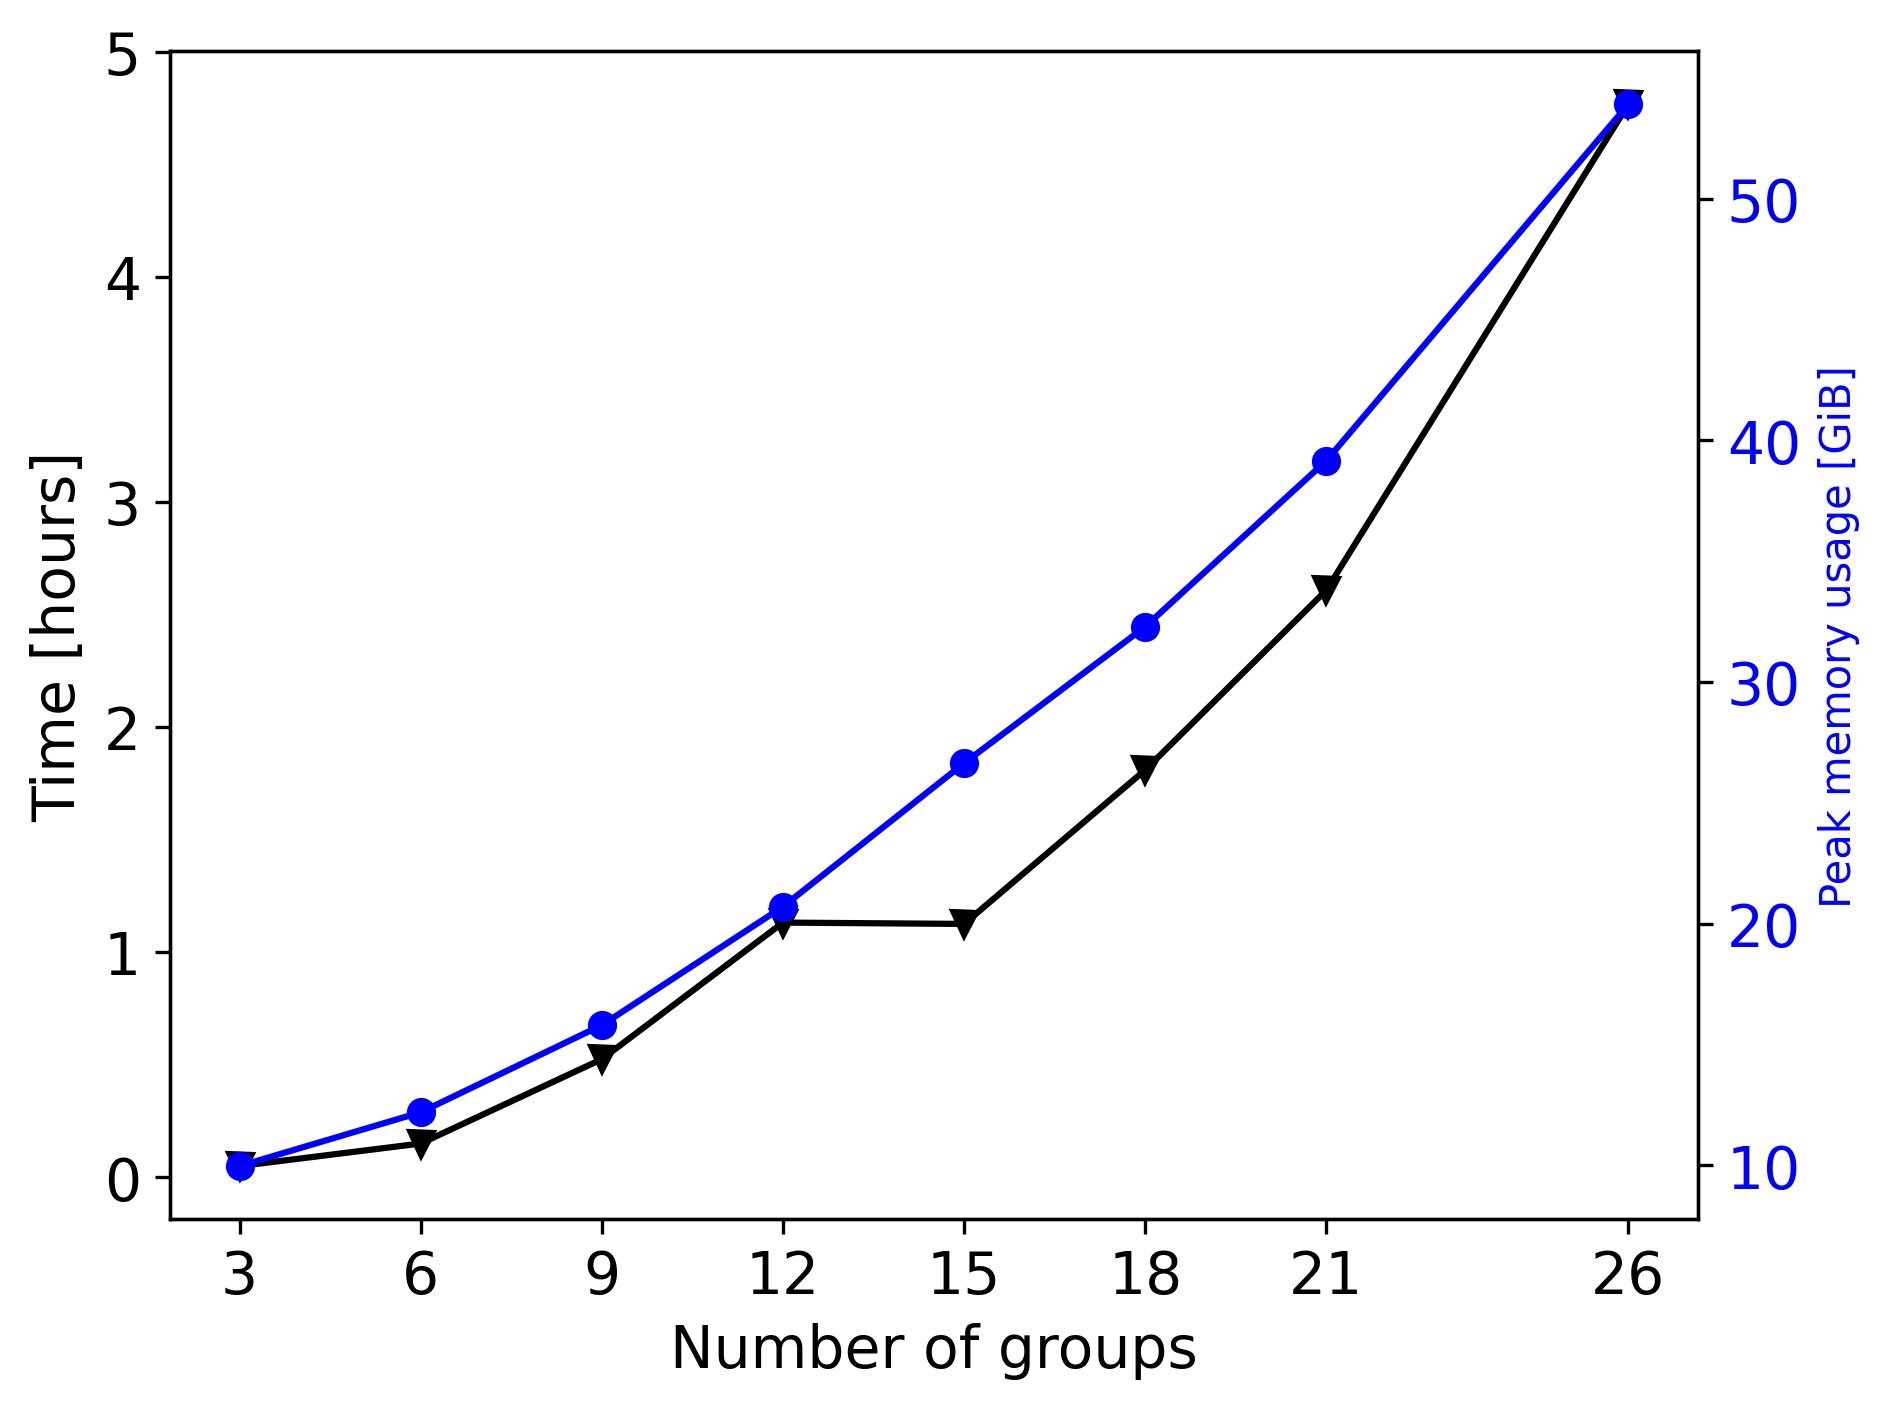
\includegraphics[width=0.45\textwidth]{figures-neutronics/time-LBP-600}
    }
	\hfill
	\caption{Computational time and memory requirements for different number of energy group structures.}
	\label{fig:assembly-time}
\end{figure}

The last study analyzed the impact of the energy group structure on the flux accuracy for a constant number of energy groups.
We chose 15 energy groups, as it yields a good overall accuracy and a practical computational expense.
Table \ref{tab:energygroups} defines the various energy group structures.
Table \ref{tab:accuracy15} exhibits the $L_2$-norm of the relative error for the various energy group structures.
Some energy group structures yield better results for some cases while giving worse results for others.
For example, the $15d$ structure gives better results at 600K with burnable poisons than without them.
To choose the best performing structure, equation \ref{eq:weighted-ave} calculated a weighted average for the different groups
\begin{align}
  & W_{ave} = w_{th} \Delta_{th} + w_{epi} \Delta_{epi} + w_{f} \Delta_{f} \label{eq:weighted-ave}
  \intertext{where}
  & W_{ave} = \mbox{weighted average } [-] \notag \\
  & w_{th} = \mbox{thermal flux weight } [-] \notag \\
  & w_{epi} = \mbox{epipthermal flux weight } [-] \notag \\
  & w_{f} = \mbox{fast flux weight } [-] \notag \\
  & \Delta_{th} = \mbox{L$_2$-norm relative difference of the thermal flux } [-] \notag \\
  & \Delta_{epi} = \mbox{L$_2$-norm relative difference of the epithermal flux } [-] \notag \\
  & \Delta_{f} = \mbox{L$_2$-norm relative difference of the fast flux } [-]. \notag
\end{align}

We arbitrarily chose the weights to be 0.5, 0.3, and 0.2 for the thermal, epithermal, and fast fluxes.
For this averaging scheme, the energy group structure $15d$ is the best one.

\begin{table}[htbp!]
  \centering
  \caption{Axial flux relative difference $L_2$-norm for various energy group structures. Values expressed in percentages.}
  \begin{tabular}{@{}l|c|l| S[table-format=2.1] S[table-format=2.1] S[table-format=2.1] S[table-format=2.1] S[table-format=2.1] }
  \toprule
	Burnable poisons     & Temperature {[}K{]}   & Flux       & \multicolumn{1}{c@{}}{15a} & \multicolumn{1}{c@{}}{15b}  & \multicolumn{1}{c@{}}{15c}  & \multicolumn{1}{c@{}}{15d}  & \multicolumn{1}{c@{}}{15e}  \\
	\midrule
	\multirow{6}{*}{No}  & \multirow{3}{*}{600}  & Fast       & 7.9  & 8.0  & 8.2  & 8.1  & 9.1  \\
	                     &                       & Epithermal & 6.6  & 6.5  & 8.6  & 8.2  & 9.2  \\
	                     &                       & Thermal    & 8.8  & 8.5  & 10.6 & 10.7 & 12.9 \\ \cline{2-8}
	                     & \multirow{3}{*}{1200} & Fast       & 7.1  & 7.7  & 5.7  & 5.1  & 4.5  \\
	                     &                       & Epithermal & 3.3  & 3.9  & 6.2  & 5.1  & 3.4  \\
	                     &                       & Thermal    & 5.0  & 4.7  & 8.5  & 8.2  & 8.4  \\ \hline
	\multirow{6}{*}{Yes} & \multirow{3}{*}{600}  & Fast       & 24.0 & 24.8 & 2.6  & 2.3  & 3.7  \\
	                     &                       & Epithermal & 21.0 & 21.7 & 2.0  & 1.6  & 2.7  \\
	                     &                       & Thermal    & 18.1 & 18.8 & 5.2  & 5.5  & 5.7  \\ \cline{2-8}
	                     & \multirow{3}{*}{1200} & Fast       & 36.2 & 37.3 & 6.9  & 6.6  & 25.9 \\
	                     &                       & Epithermal & 33.2 & 34.2 & 6.9  & 6.5  & 25.1 \\
	                     &                       & Thermal    & 29.6 & 30.6 & 8.5  & 8.3  & 20.3 \\
	\midrule
	\multicolumn{2}{l}{Weighted average}         &            & 17.3 & 17.8 & 6.3  & 6.0  & 10.8 \\
	\bottomrule
  \end{tabular}
  \label{tab:accuracy15}
\end{table}


\subsection{Full-core}

This section compared the results from Serpent and Moltres simulations of a full-core model.
Figure \ref{fig:fullcoremodel} displays a $xy$-plane of the model, which includes the bottom and top reflectors.
Due to symmetry, Moltres model included only a $1/6^{th}$ of the reactor.
The first step in the calculation obtained the group constants using Serpent.
Tables \ref{tab:maincharac}, \ref{tab:element-characteristics}, and \ref{tab:compact} specify the model input parameters.
For simplicity, standard fuel assemblies compose all the fuel column.
The model considered a fresh core, and it did not include the fuel handling holes nor the bottom and top reflector coolant channels.
Based on the previous section analyses, we chose the energy group structure $15d$ in Table \ref{tab:energygroups}.
The material temperatures were 600K and 1200K, cases that represent the \gls{CZP} and the \gls{HFP} core states.
The Serpent simulations included 8$\times 10^5$ neutrons per cycle, 500 active cycles, and 100 inactive cycles.

% Geometries
\begin{figure}[htbp!]
	\centering
    \subfloat[Serpent model geometry.]{
        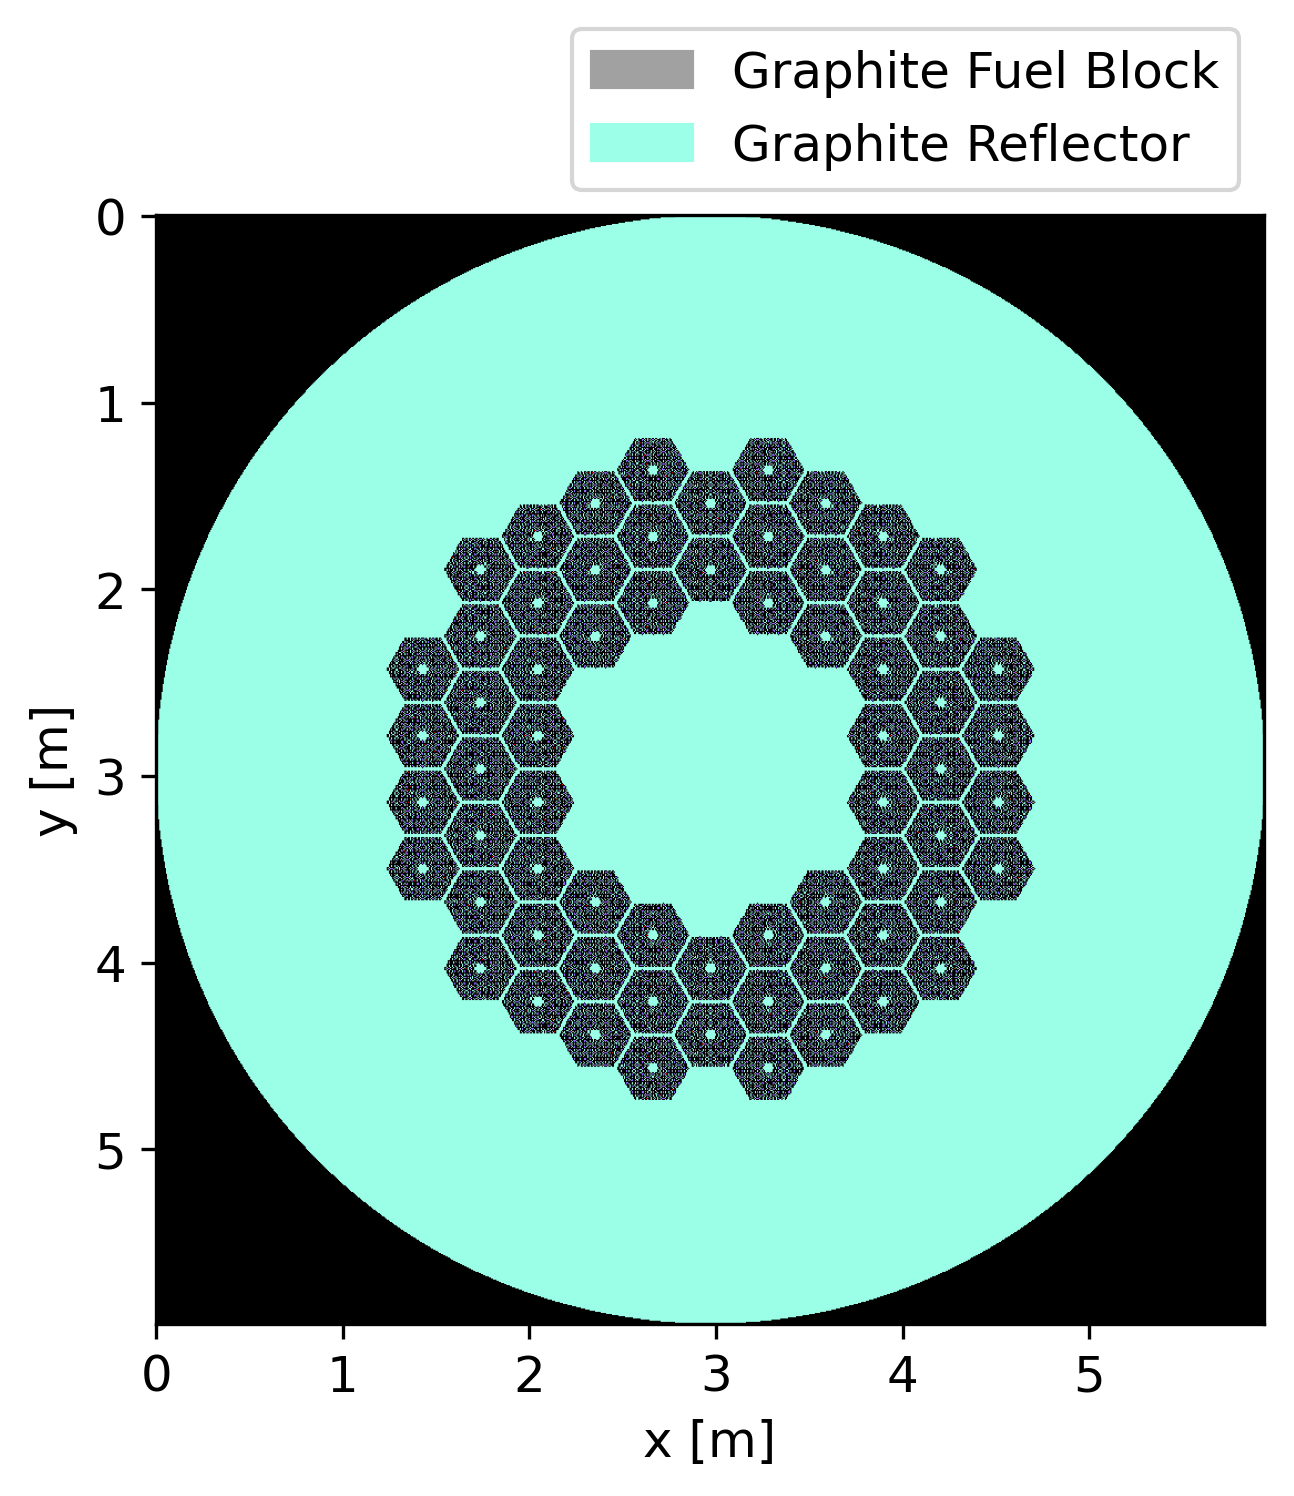
\includegraphics[width=0.39\textwidth]{figures-neutronics/oecd-fullcore}
    }
    \subfloat[Moltres model geometry.]{
        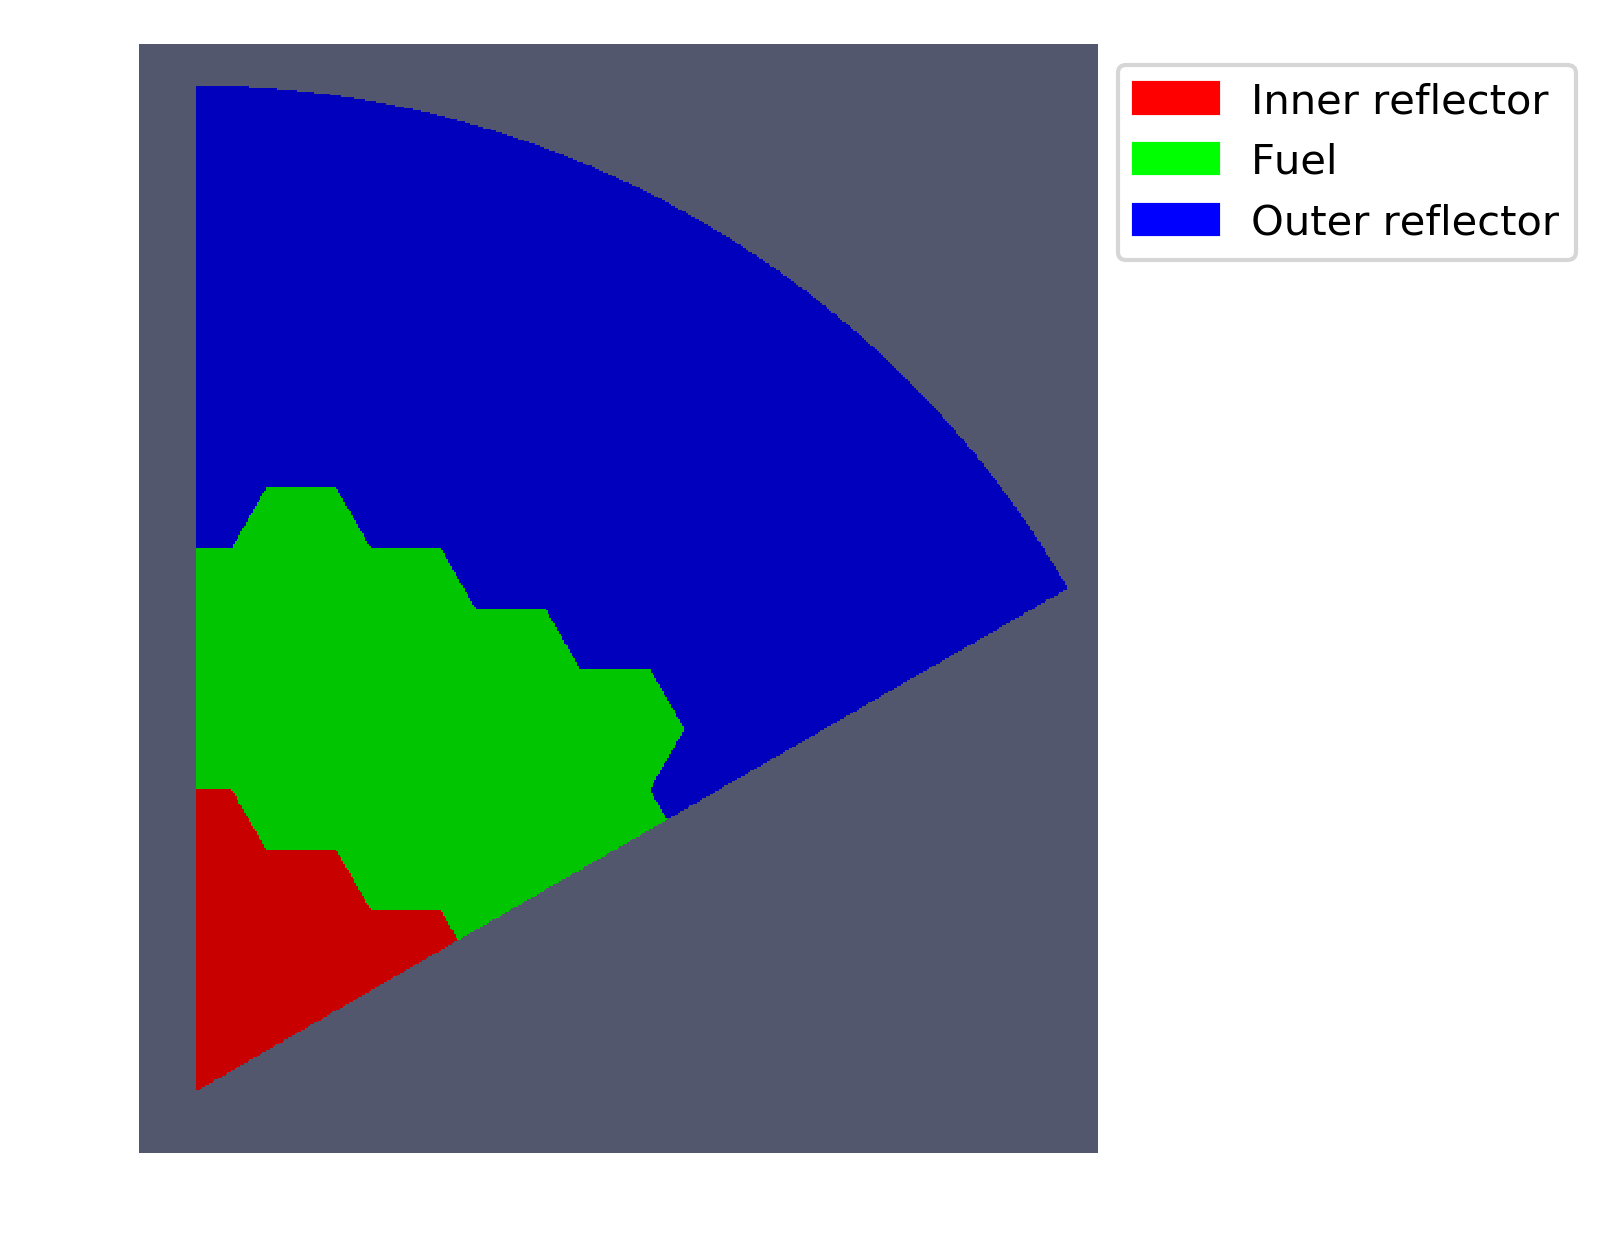
\includegraphics[width=0.49\textwidth]{figures-neutronics/3D-fullcore-60-homo-meshB2}
    }
	\hfill
  \caption{MHTGR-350 full-core model layout.}
	\label{fig:fullcoremodel}
\end{figure}

Moltres model geometry and mesh, which had 3.0 $\times 10^5$ elements and 1.60 $\times 1-^5$ nodes, using Gmsh.
The diffusion calculations had 1.60 $\times 10^5$ \glspl{DoF} per energy-group and a total of 2.4 $\times 10^6$ DoFs.
The Moltres input files set an eigenvalue and a flux convergence tolerance of 1$\times$10$^{-8}$.

% Keff
Between Serpent and Moltres, we compared the \gls{Keff}, the power distribution, and the flux shape and magnitude in different zones of the reactor.
Table \ref{tab:full-keff} exhibits the \gls{Keff} from Serpent and Moltres.
The differences between the eigenvalues calculated by Moltres and Serpent are smaller than 300 pcm.

\begin{table}[htbp!]
  \centering
  \caption{Comparison between Serpent and Moltres-derived eigenvalues.}
  \begin{tabular}{cccc}
  \toprule
  Temperature [K] & Serpent			     & Moltres  & $\Delta \rho$ [pcm] 	\\
  \midrule
			 600  	    & 1.10869 $\pm$ 0.00006  & 1.11150	 &	228		\\
			1200 	      & 1.06138 $\pm$ 0.00006  & 1.06468	 &	292   \\
  \bottomrule
  \end{tabular}
  \label{tab:full-keff}
\end{table}

% Power distribution
Figures \ref{fig:fullcore-600-power} and \ref{fig:fullcore-1200-power} show Serpent and Moltres radial power distributions.
The following analysis applies to both temperatures.
Regarding the power distribution, the results are symmetric with respect to a 60$^{\circ}$ line.
This suggests that we could reduce the mesh size by almost half by considering only $1/12^{th}$ of the reactor.
Next, we observe that Moltres result exhibits a higher power density than Serpent in the inner and outer rings but a lower power density in the middle ring.
The largest difference occurs at 600K, shown Figure \ref{fig:fullcore-600-power}, in the inner ring and has a magnitude of 0.29 MW.

%Power distribution at 600K
\begin{figure}[htbp!]
	\centering
    \subfloat[Serpent radial power distribution.]{
        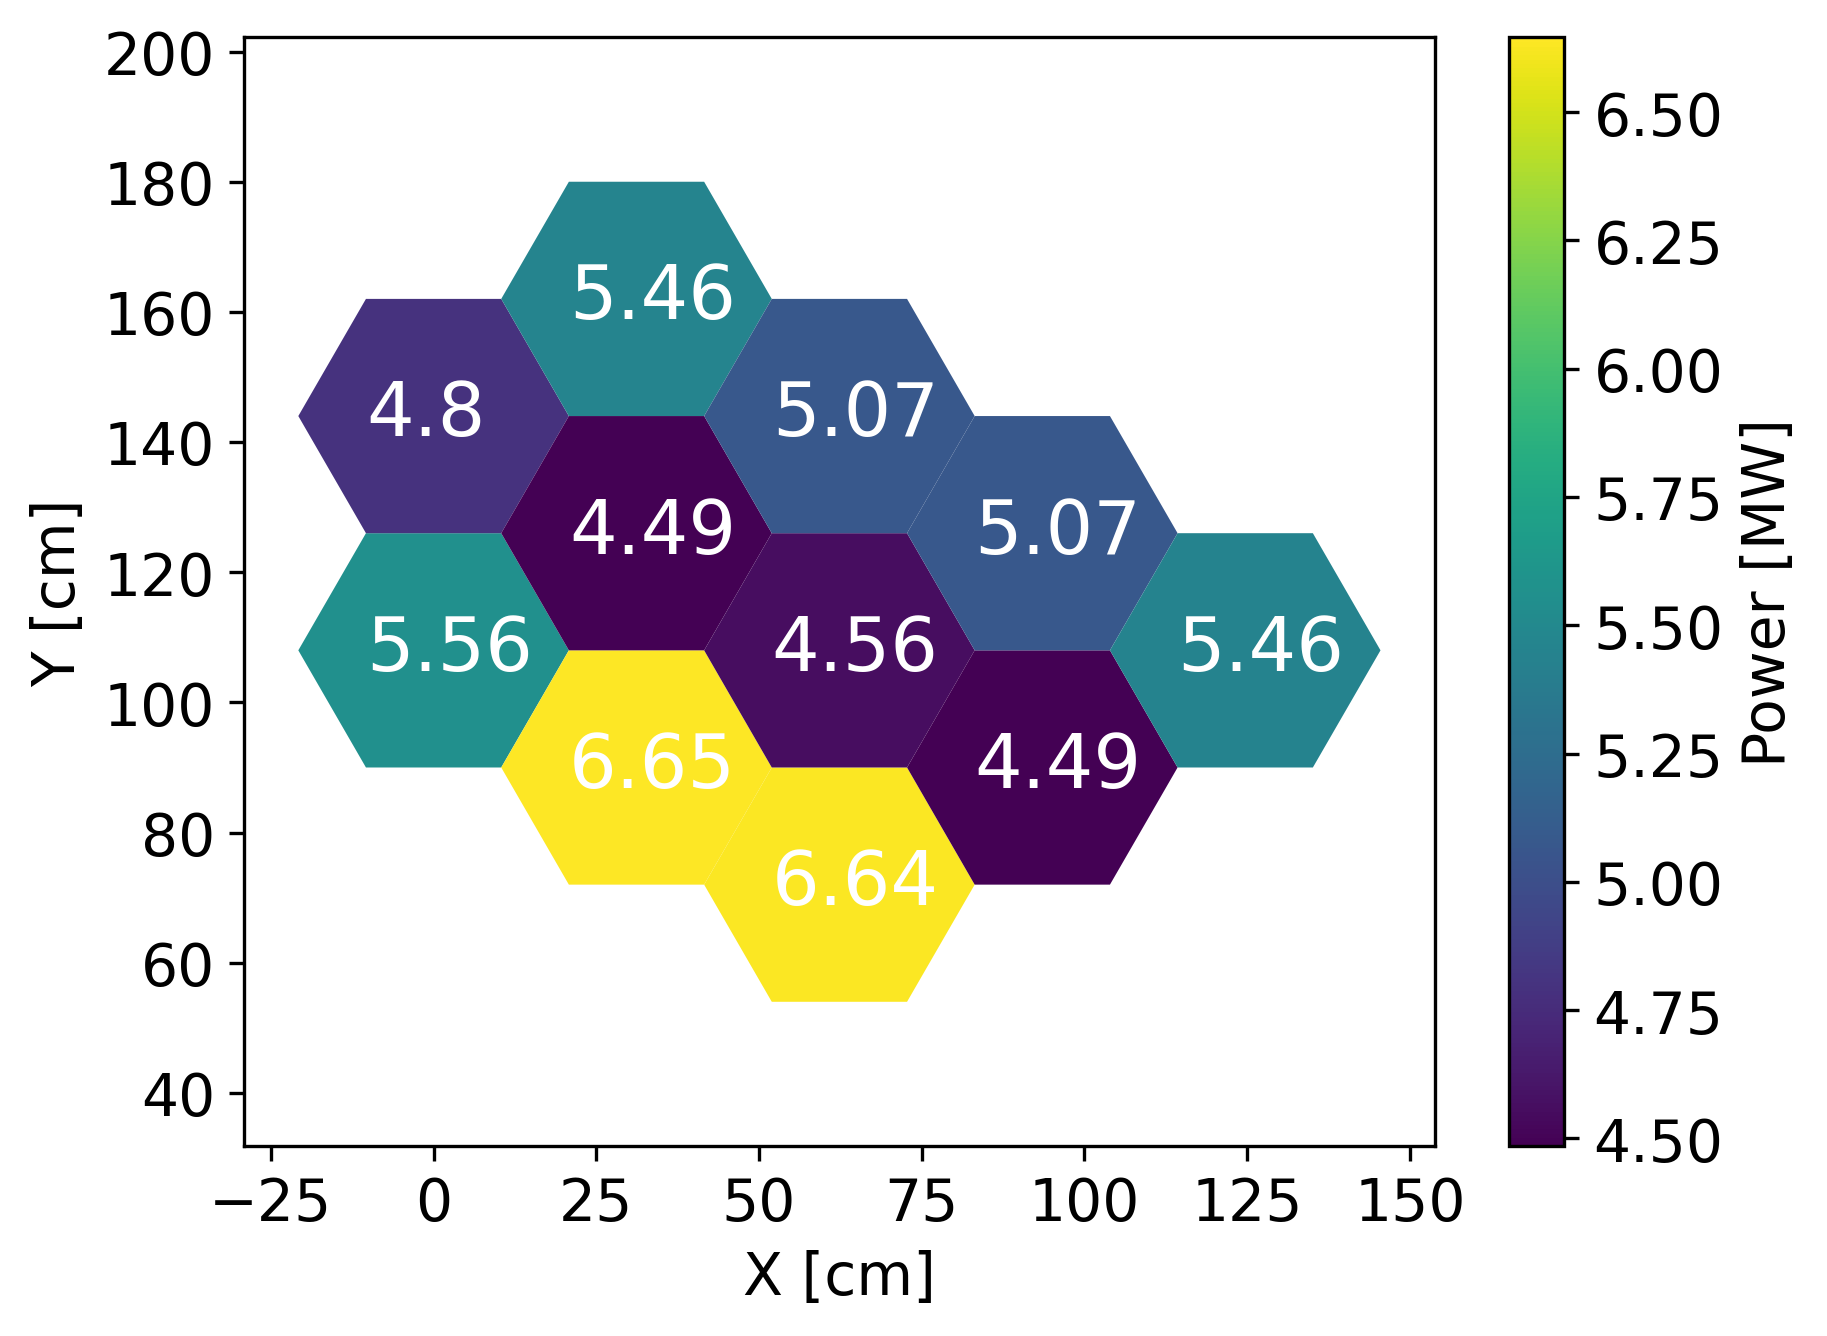
\includegraphics[width=0.45\textwidth]{figures-neutronics/serpent26G-600-power}
    }
    \subfloat[Moltres radial power distribution.]{
        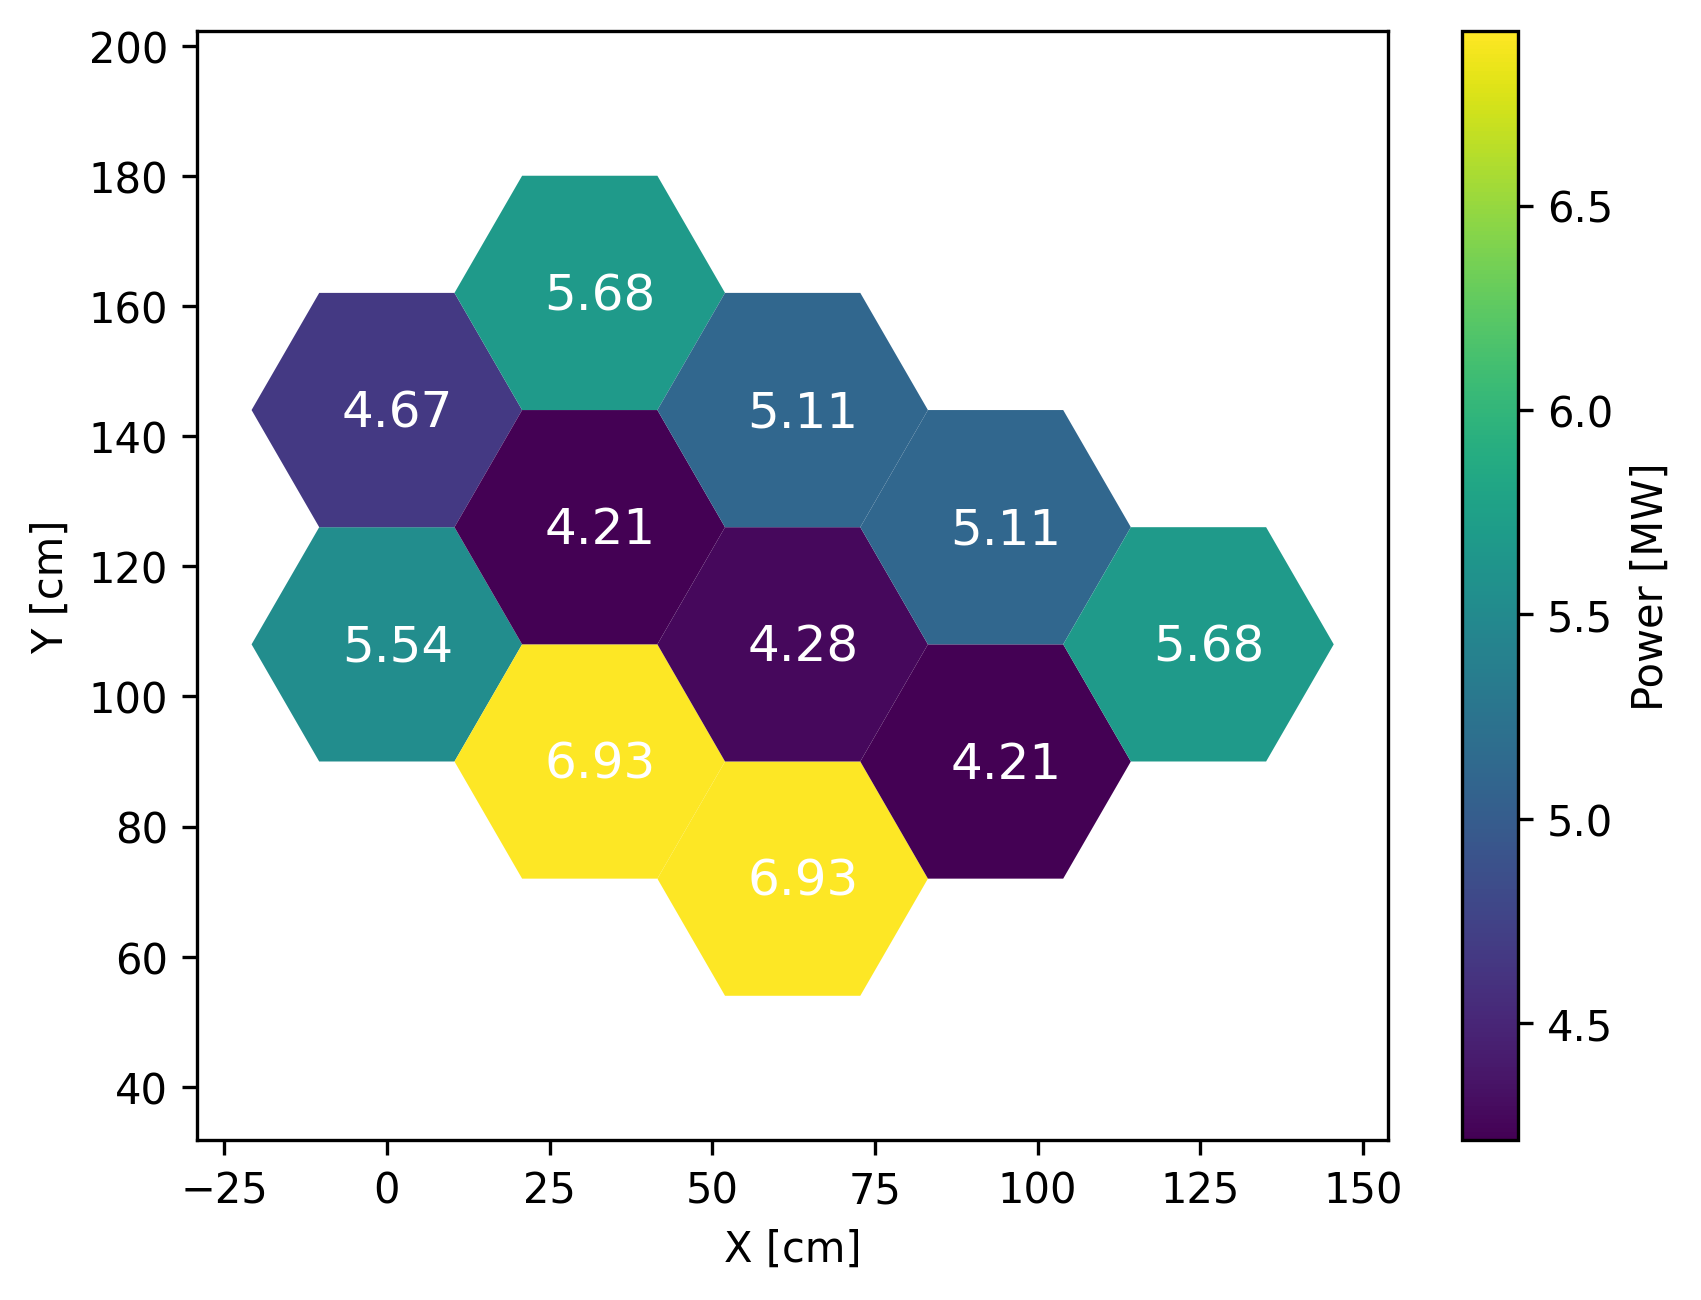
\includegraphics[width=0.45\textwidth]{figures-neutronics/3D-fullcore-600-15Gd-power}
    }
	\hfill
	\caption{Comparison of the MHTGR-350 radial power distribution at 600 K calculated by Serpent and Moltres.}
	\label{fig:fullcore-600-power}
\end{figure}

%Power distribution at 1200K
\begin{figure}[htbp!]
	\centering
    \subfloat[Serpent radial power distribution.]{
        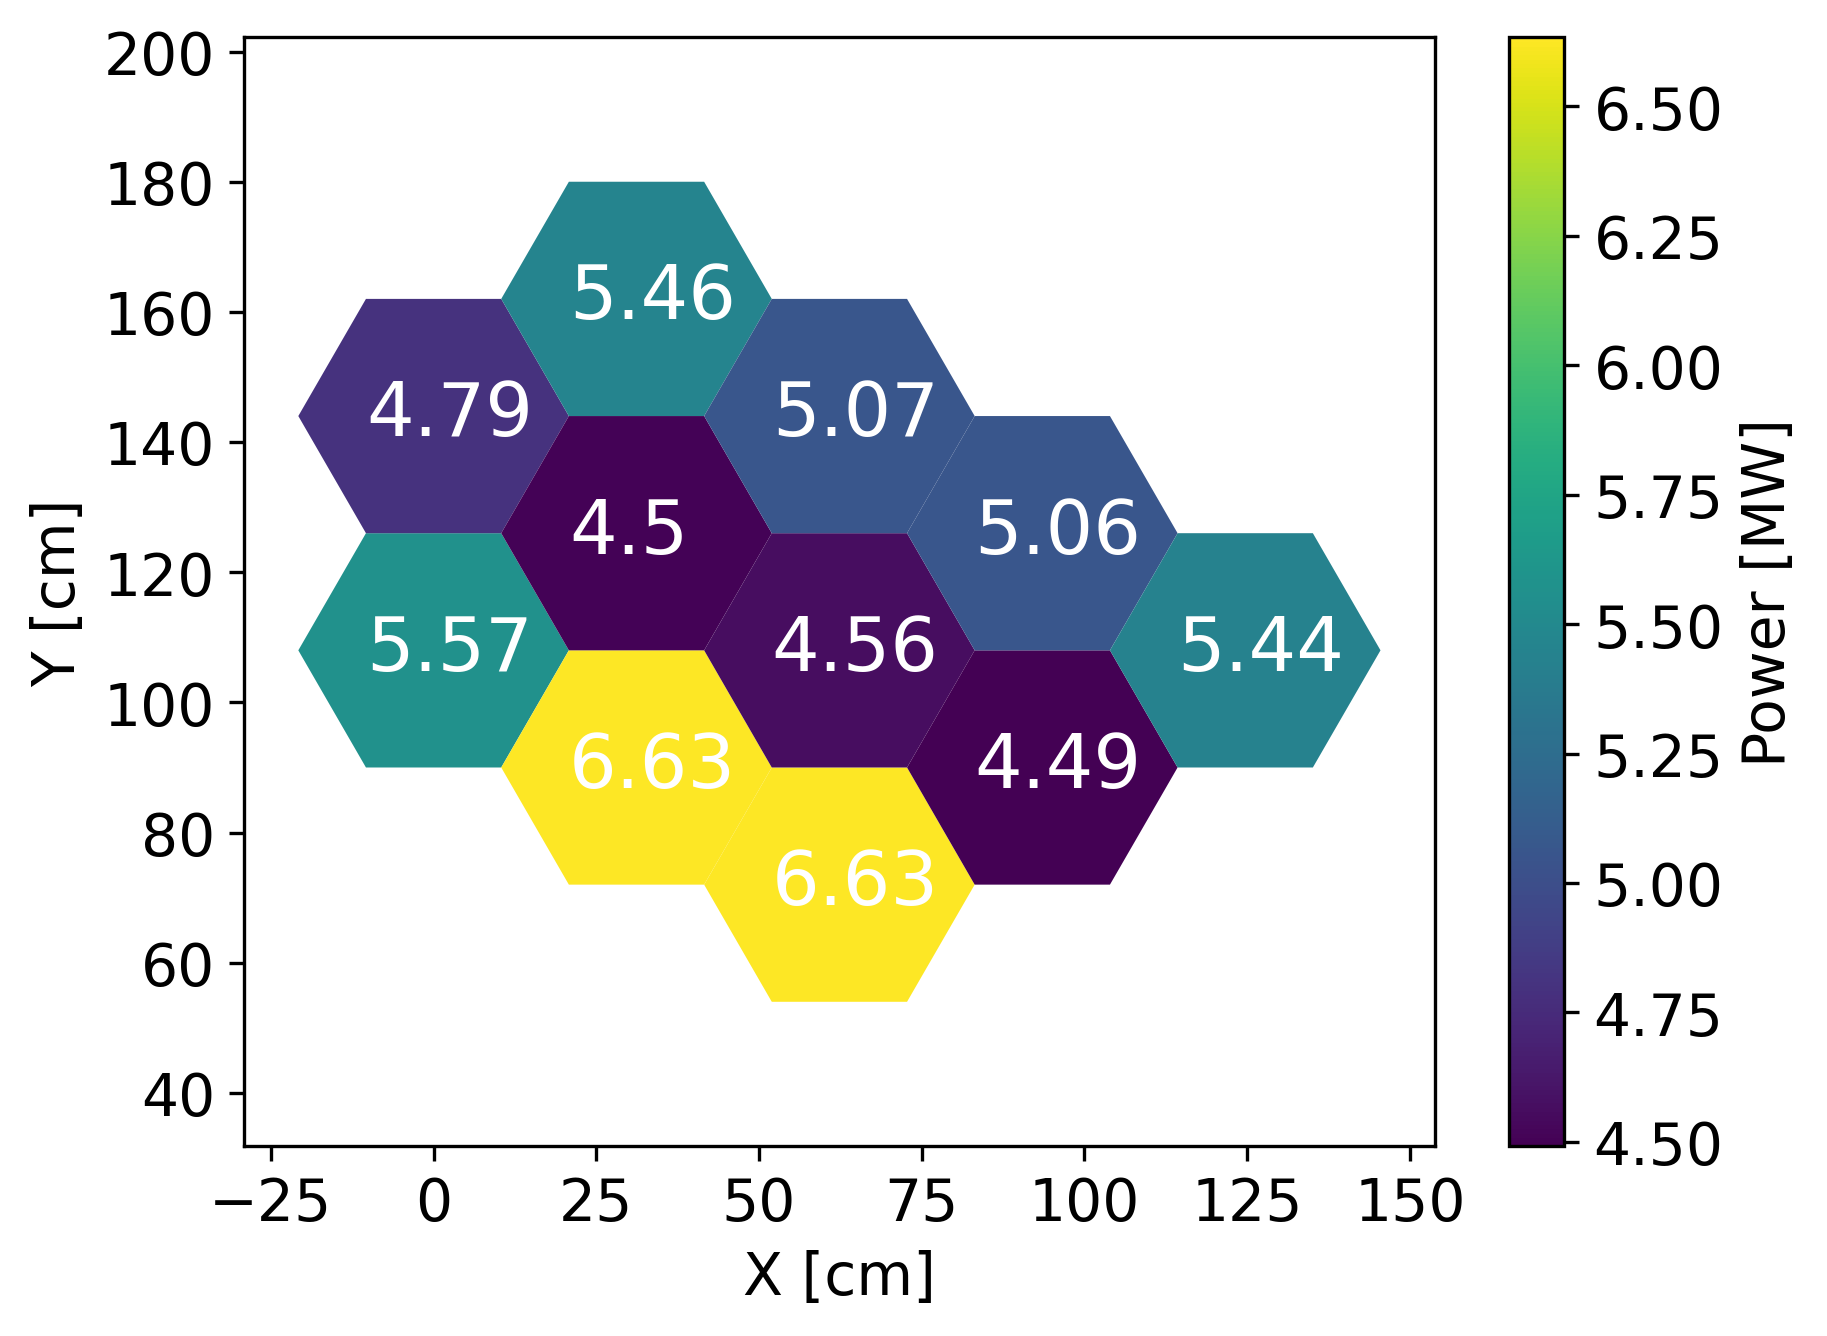
\includegraphics[width=0.45\textwidth]{figures-neutronics/serpent26G-1200-power}
    }
    \subfloat[Moltres radial power distribution.]{
        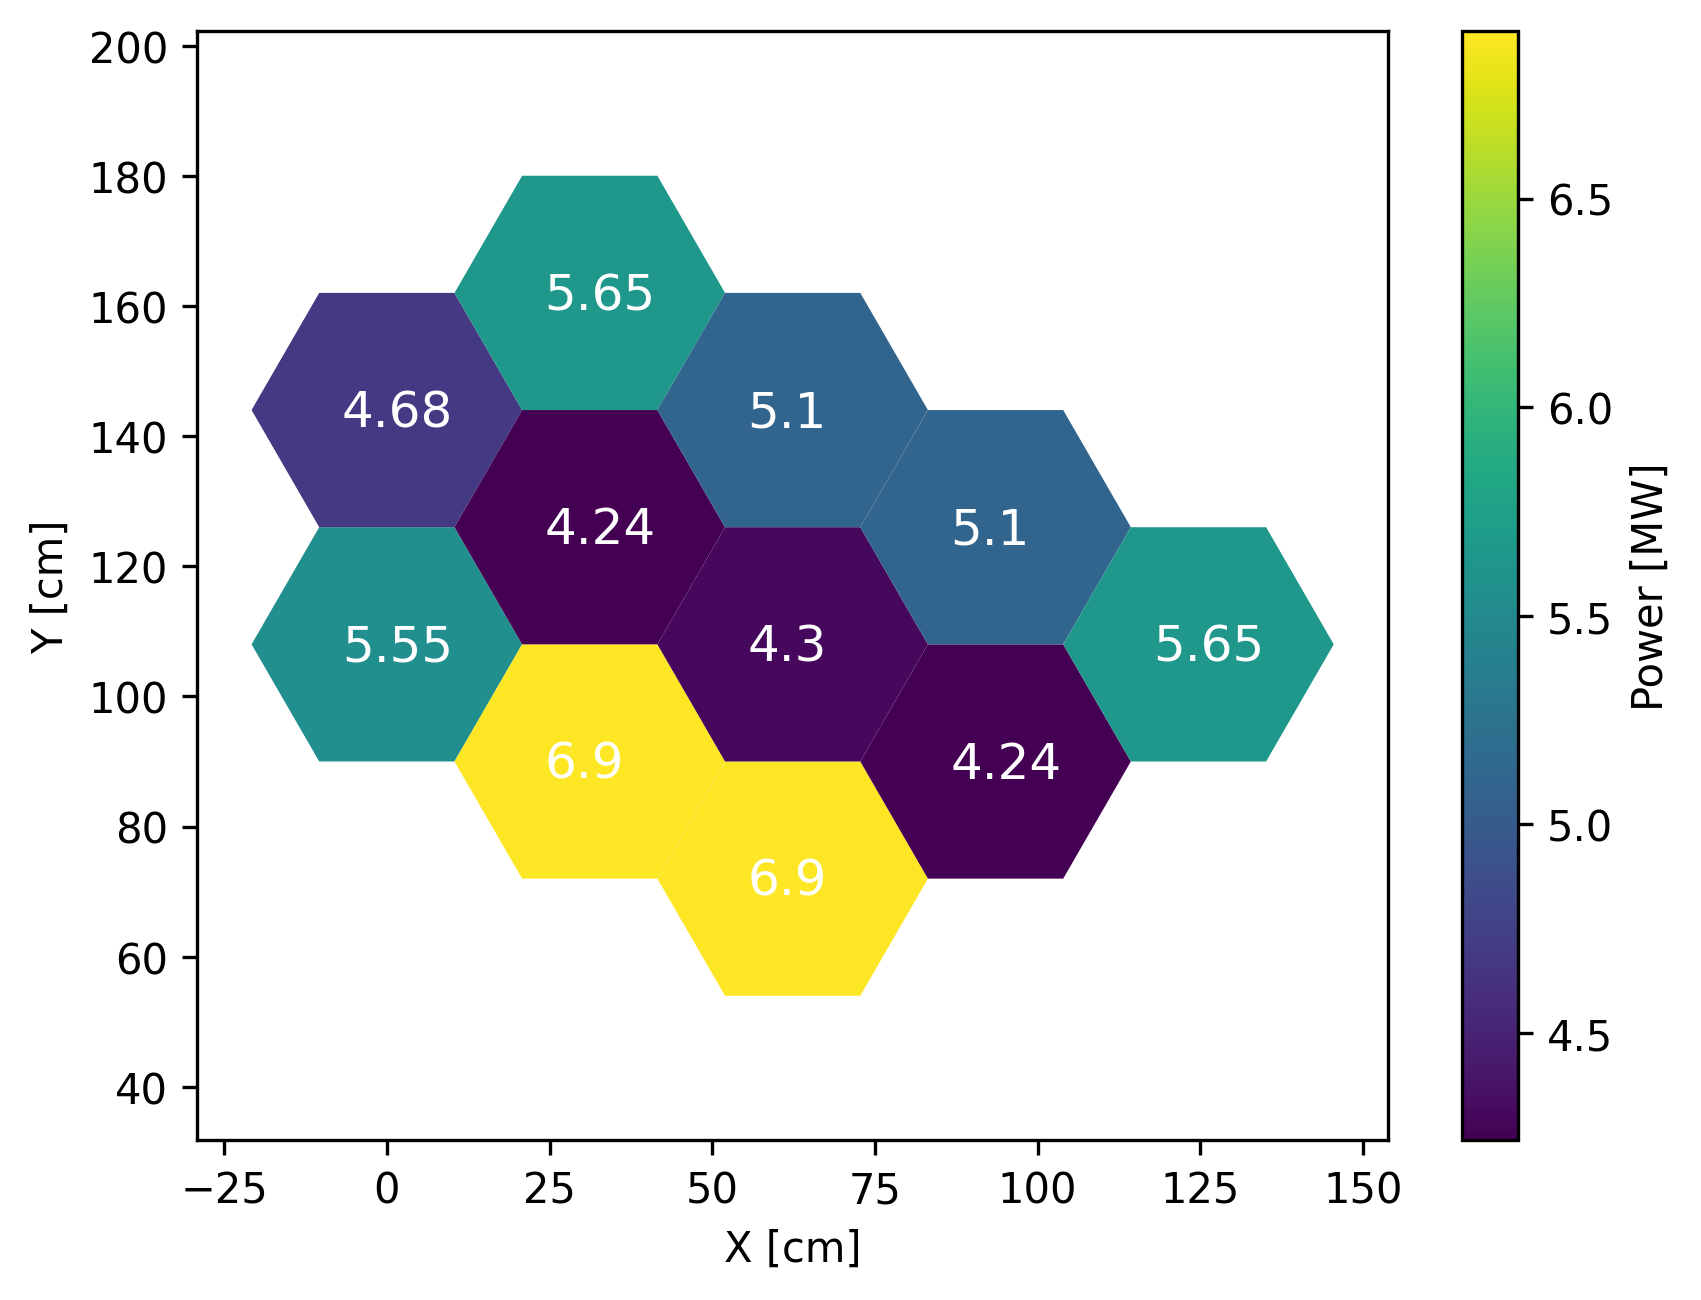
\includegraphics[width=0.45\textwidth]{figures-neutronics/3D-fullcore-1200-15Gc-power}
    }
	\hfill
	\caption{Comparison of the MHTGR-350 radial power distribution at 1200 K calculated by Serpent and Moltres.}
	\label{fig:fullcore-1200-power}
\end{figure}

% Fluxes
We placed axial and radial flux detectors in arbitrary regions of the reactor to compare the fluxes, Figure \ref{fig:fullcore-detectors} shows their locations.
Both the Serpent and Moltres radial detector's axial location was the middle of the active core's height.
Note that the flux in Serpent is an average over the fuel column's volume, while the flux in Moltres is the point-wise flux over the fuel column's centerline.
The Serpent radial detector's volume had a 2$^{\circ}$-angle and a fuel assembly's height.
Moltres ran the calculations for 15 energy groups and collapsed the results into three groups to facilitate the results' visualization.
Figures \ref{fig:fullcore-600-axial1} and \ref{fig:fullcore-600-radial1} show the axial and radial fluxes at 600K.
The axial flux shapes are similar, but Figure \ref{fig:fullcore-600-axial1} shows that the fast and epithermal axial fluxes in Moltres are larger, while the axial thermal flux is smaller.
The axial epithermal and thermal fluxes are closer in magnitude in the active core in Serpent's simulation.
In Figure \ref{fig:fullcore-600-radial1}, Serpent fluxes present some 'noise.'
A higher number of generations per cycle in Serpent simulations or using a detector with a larger volume would eliminate this.
Additionally, the radial flux in Serpent reveals the location of the burnable poisons in the fuel assemblies.
This diffusion simulation fails to capture such localized effects as the group constants are homogeneous in the fuel assembly.
The radial fast flux in Moltres is larger, while the radial epithermal and thermal fluxes have almost the same magnitudes.
Figures \ref{fig:fullcore-1200-axial1} and \ref{fig:fullcore-1200-radial1} display the fluxes at 1200K, which differ from the 600K case.
Still, we observe the same behavior for both axial and radial fluxes.
Overall, Moltres and Serpent fluxes are comparable in magnitude and shape.

%Detectors
\begin{figure}[htbp!]
	\centering
    \subfloat[Flux detectors in Serpent model.]{
        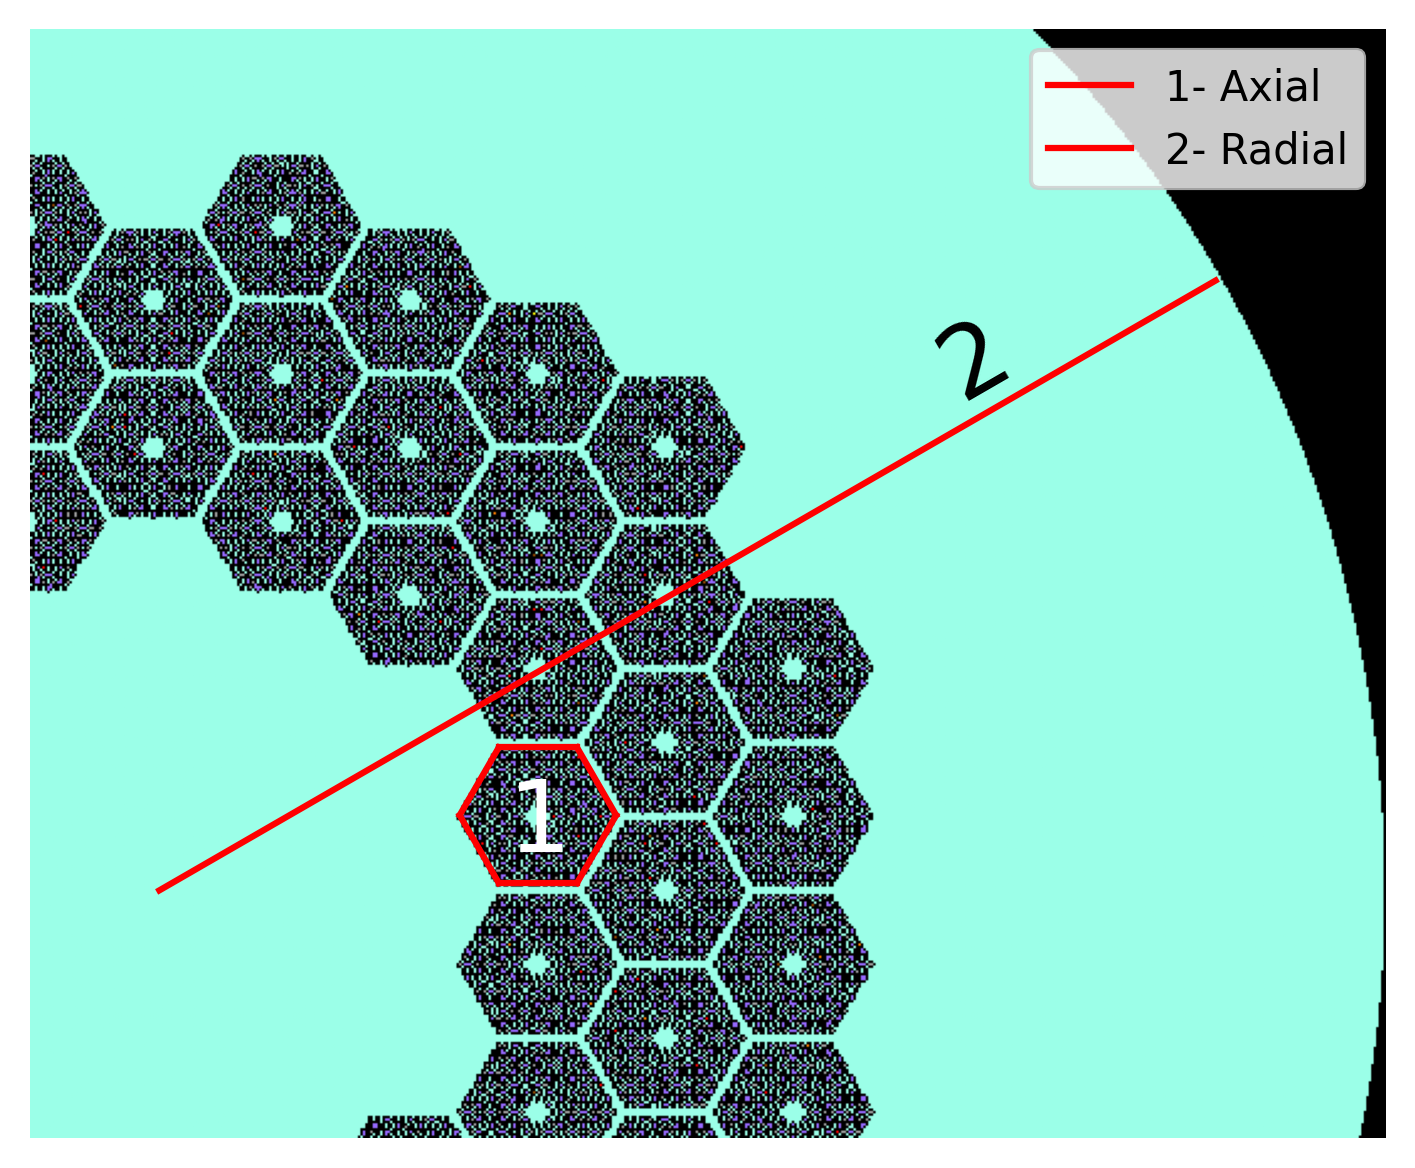
\includegraphics[width=0.52\textwidth]{figures-neutronics/oecd-fullcore-detectorsC}
    }
    \subfloat[Flux detectors in Moltres model.]{
        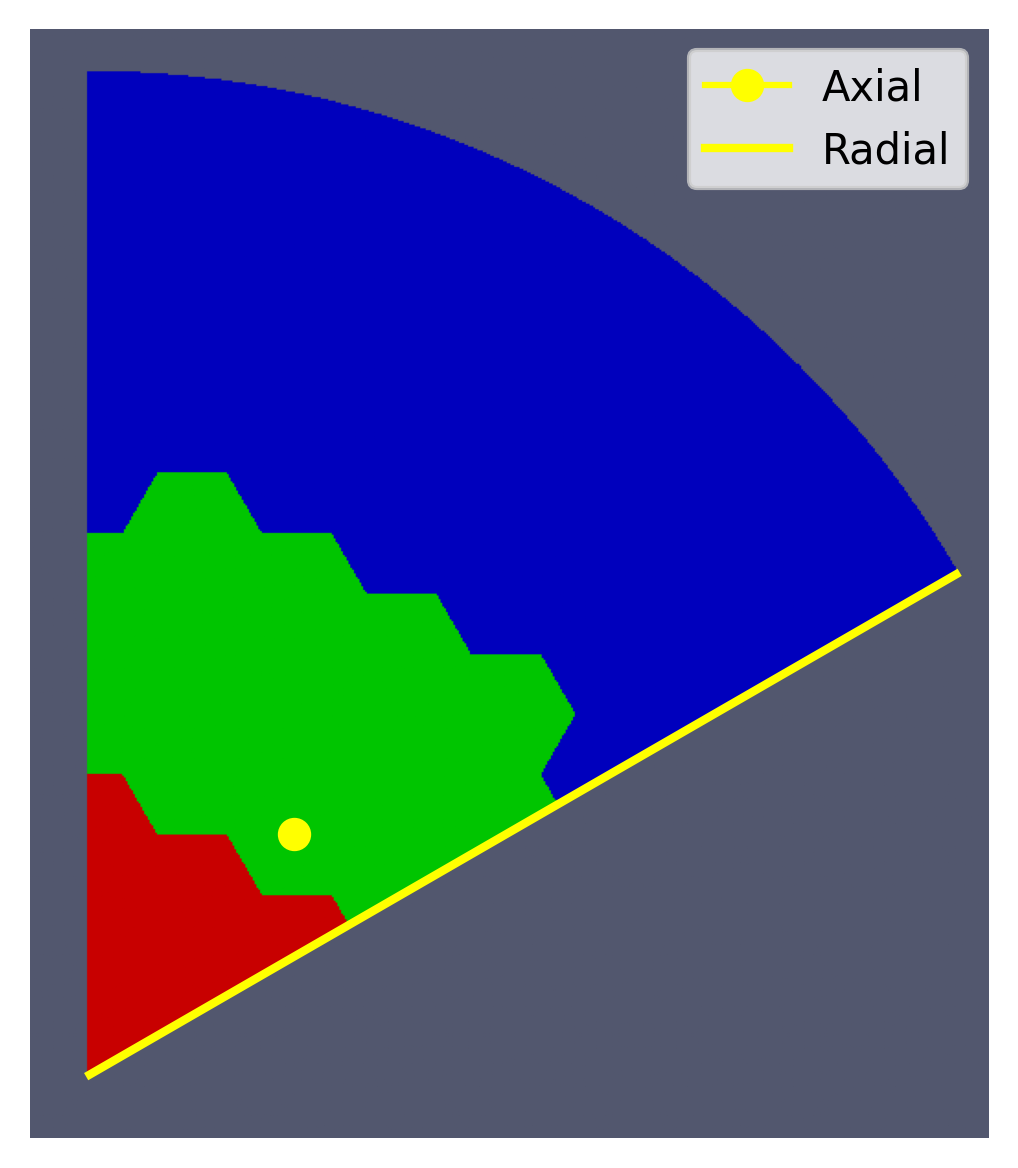
\includegraphics[width=0.37\textwidth]{figures-neutronics/3D-fullcore-60-detectors2}
    }
	\hfill
	\caption{Axial view of the flux detector locations.}
	\label{fig:fullcore-detectors}
\end{figure}

% Axial flux1 at 600K
\begin{figure}[htbp!]
	\centering
    \subfloat[Serpent axial detector flux.]{
        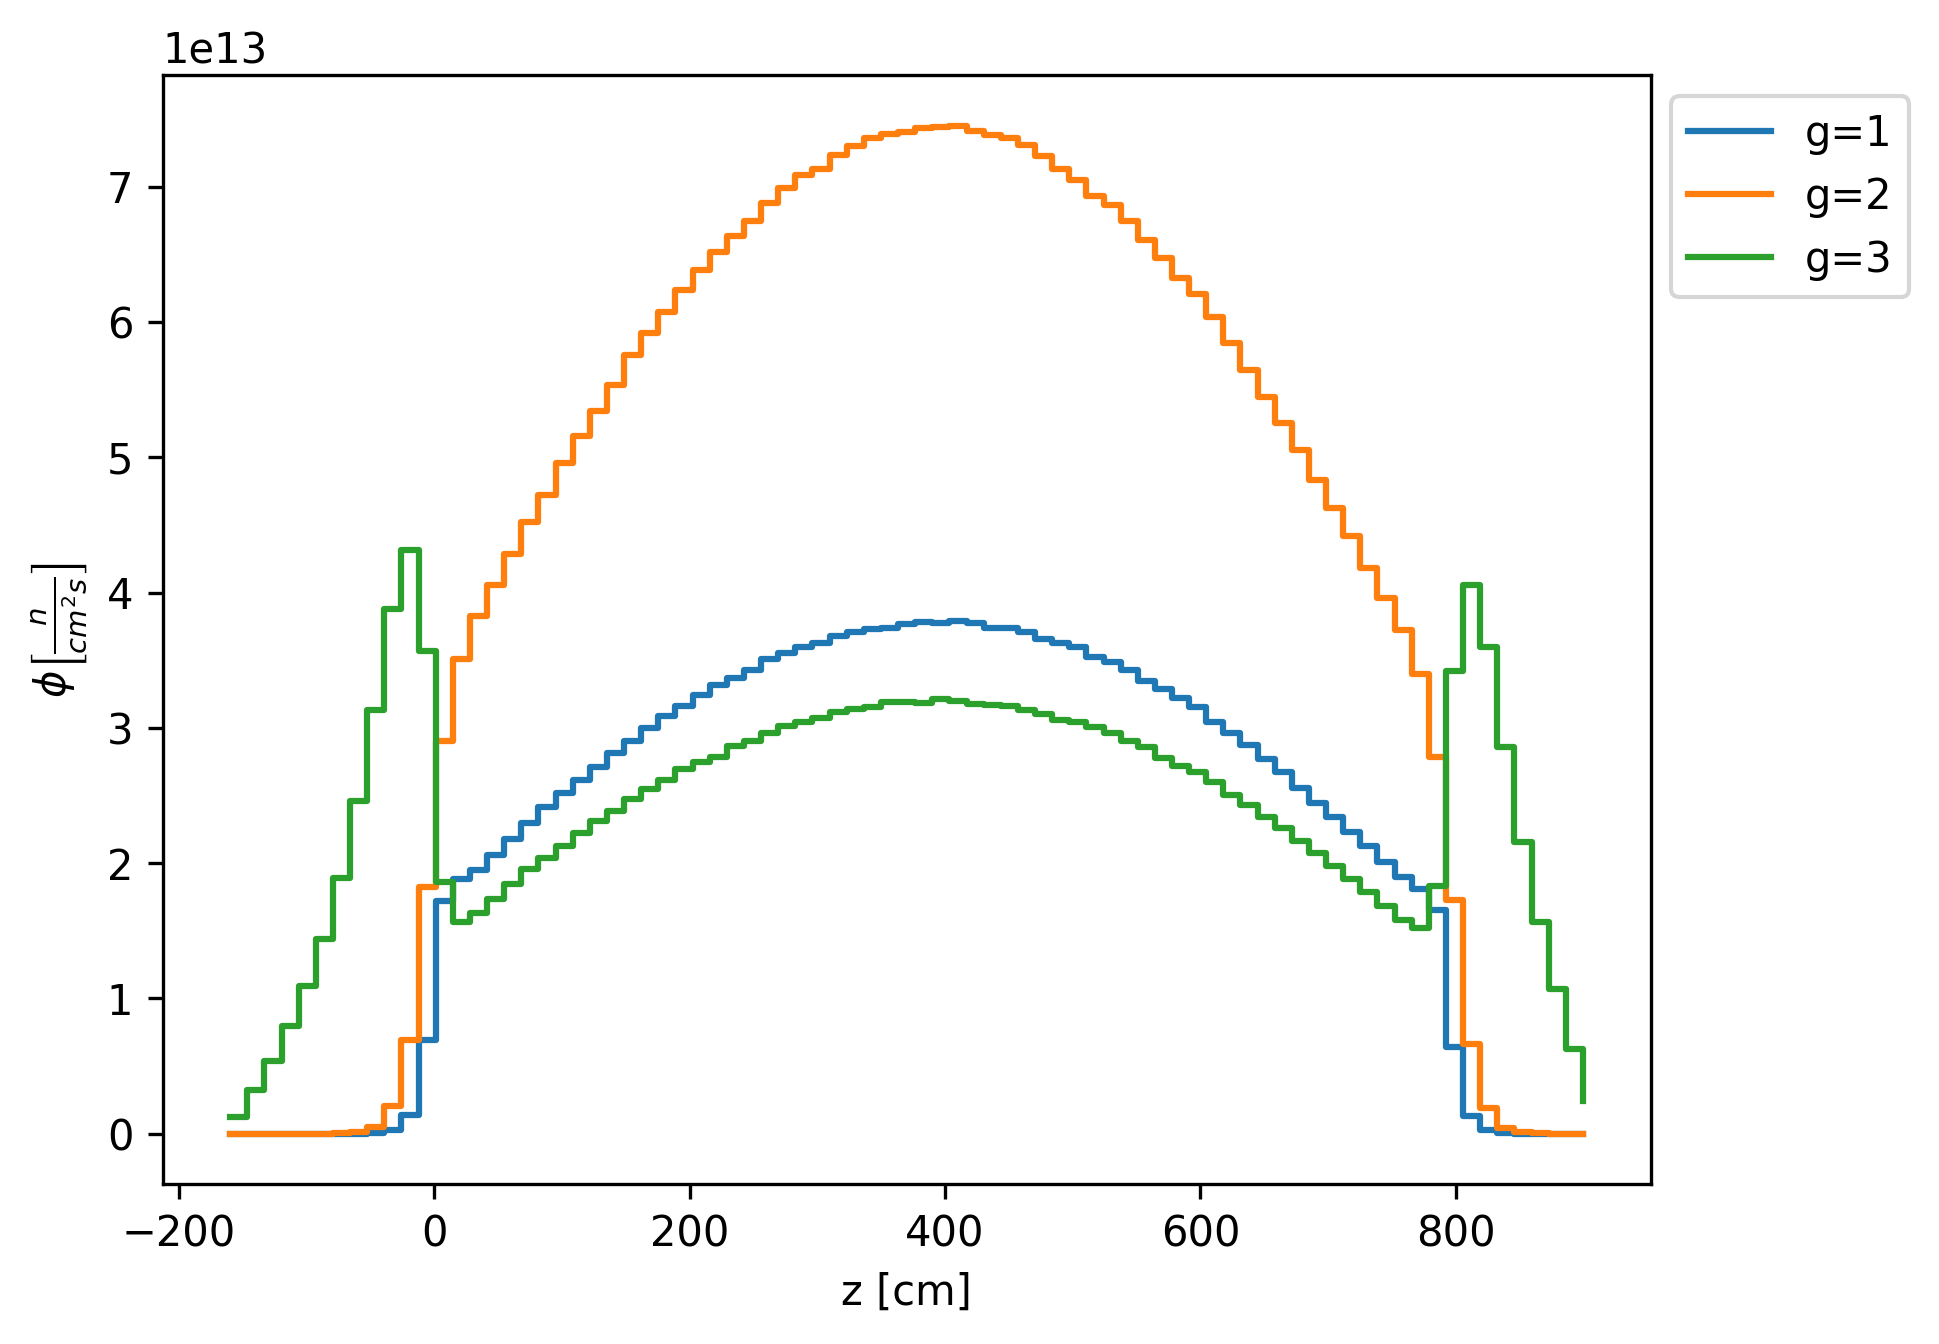
\includegraphics[width=0.45\textwidth]{figures-neutronics/serpent26G-600-collapse-Axial1}
    }
    \subfloat[Moltres axial detector flux.]{
        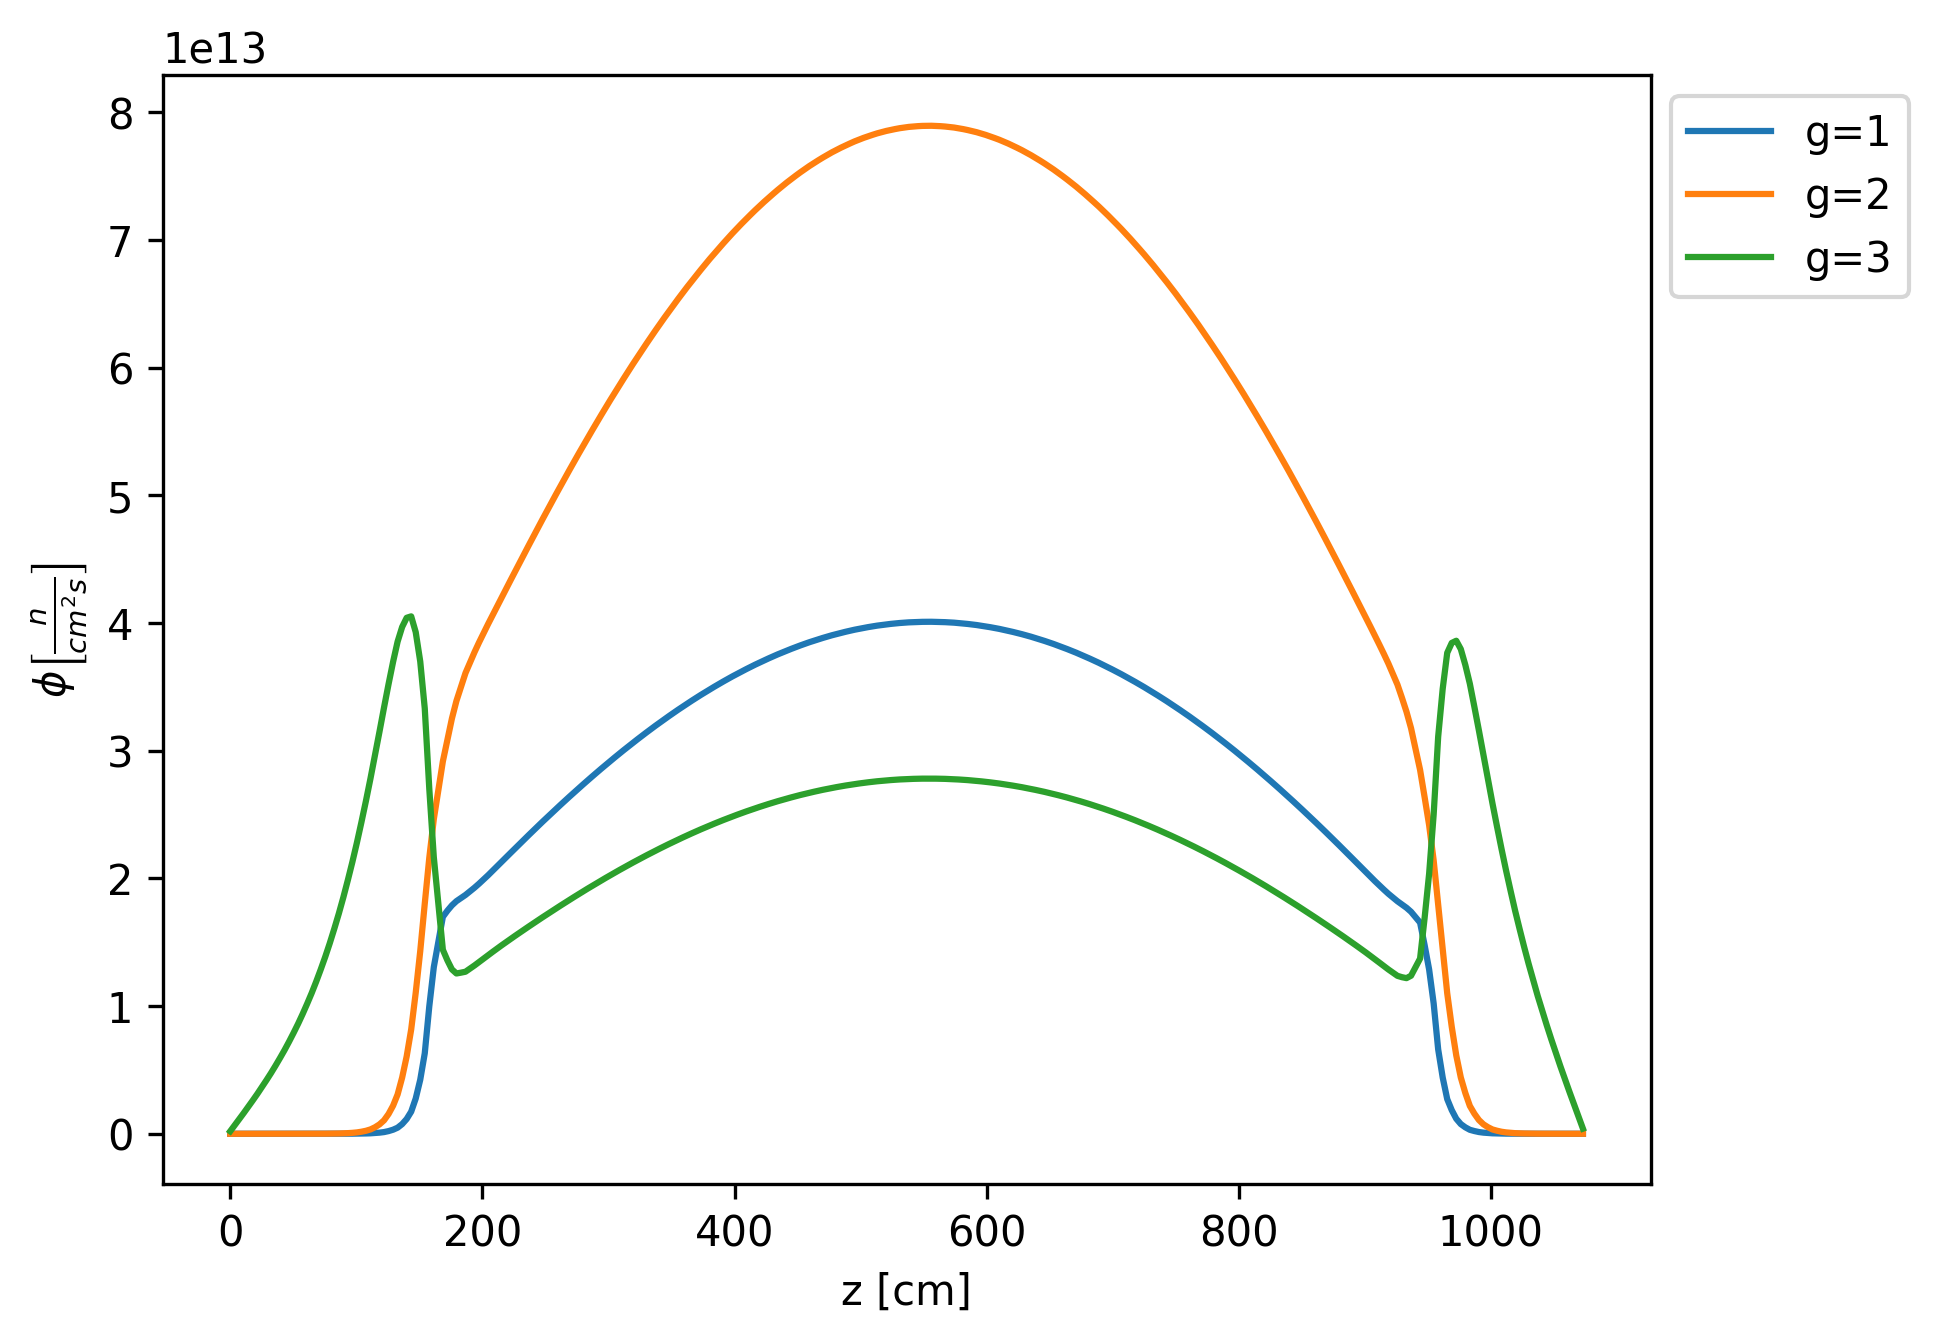
\includegraphics[width=0.45\textwidth]{figures-neutronics/3D-fullcore-600-15Gd-axial1}
    }
	\hfill
	\caption{Comparison of the axial detector flux calculated by Serpent and Moltres at 600 K.}
	\label{fig:fullcore-600-axial1}
\end{figure}

%Radial flux at 600 K
\begin{figure}[htbp!]
	\centering
    \subfloat[Serpent radial detector flux.]{
        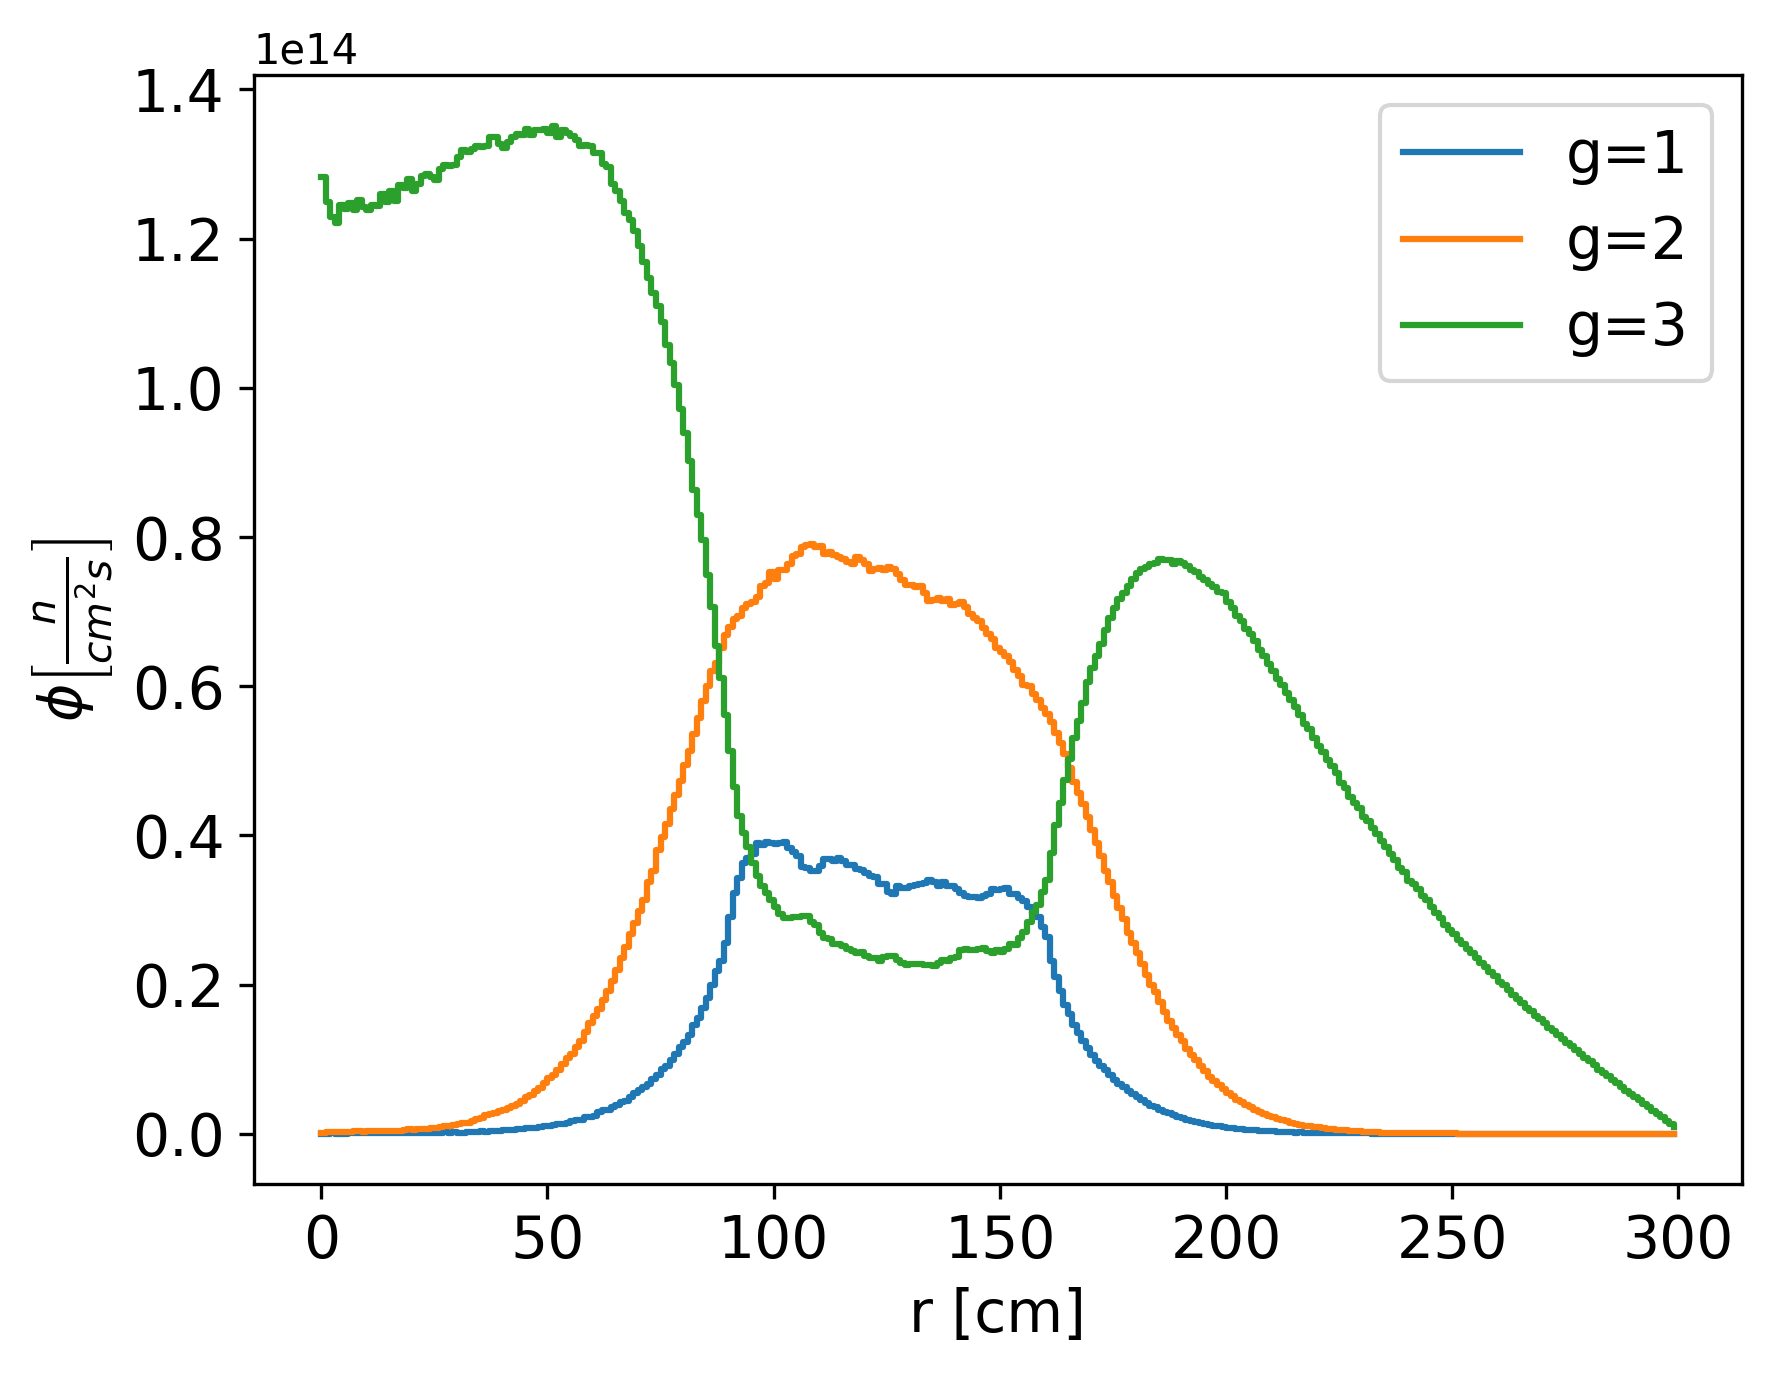
\includegraphics[width=0.45\textwidth]{figures-neutronics/serpent26G-600-collapse-Radial}
    }
    \subfloat[Moltres radial detector flux.]{
        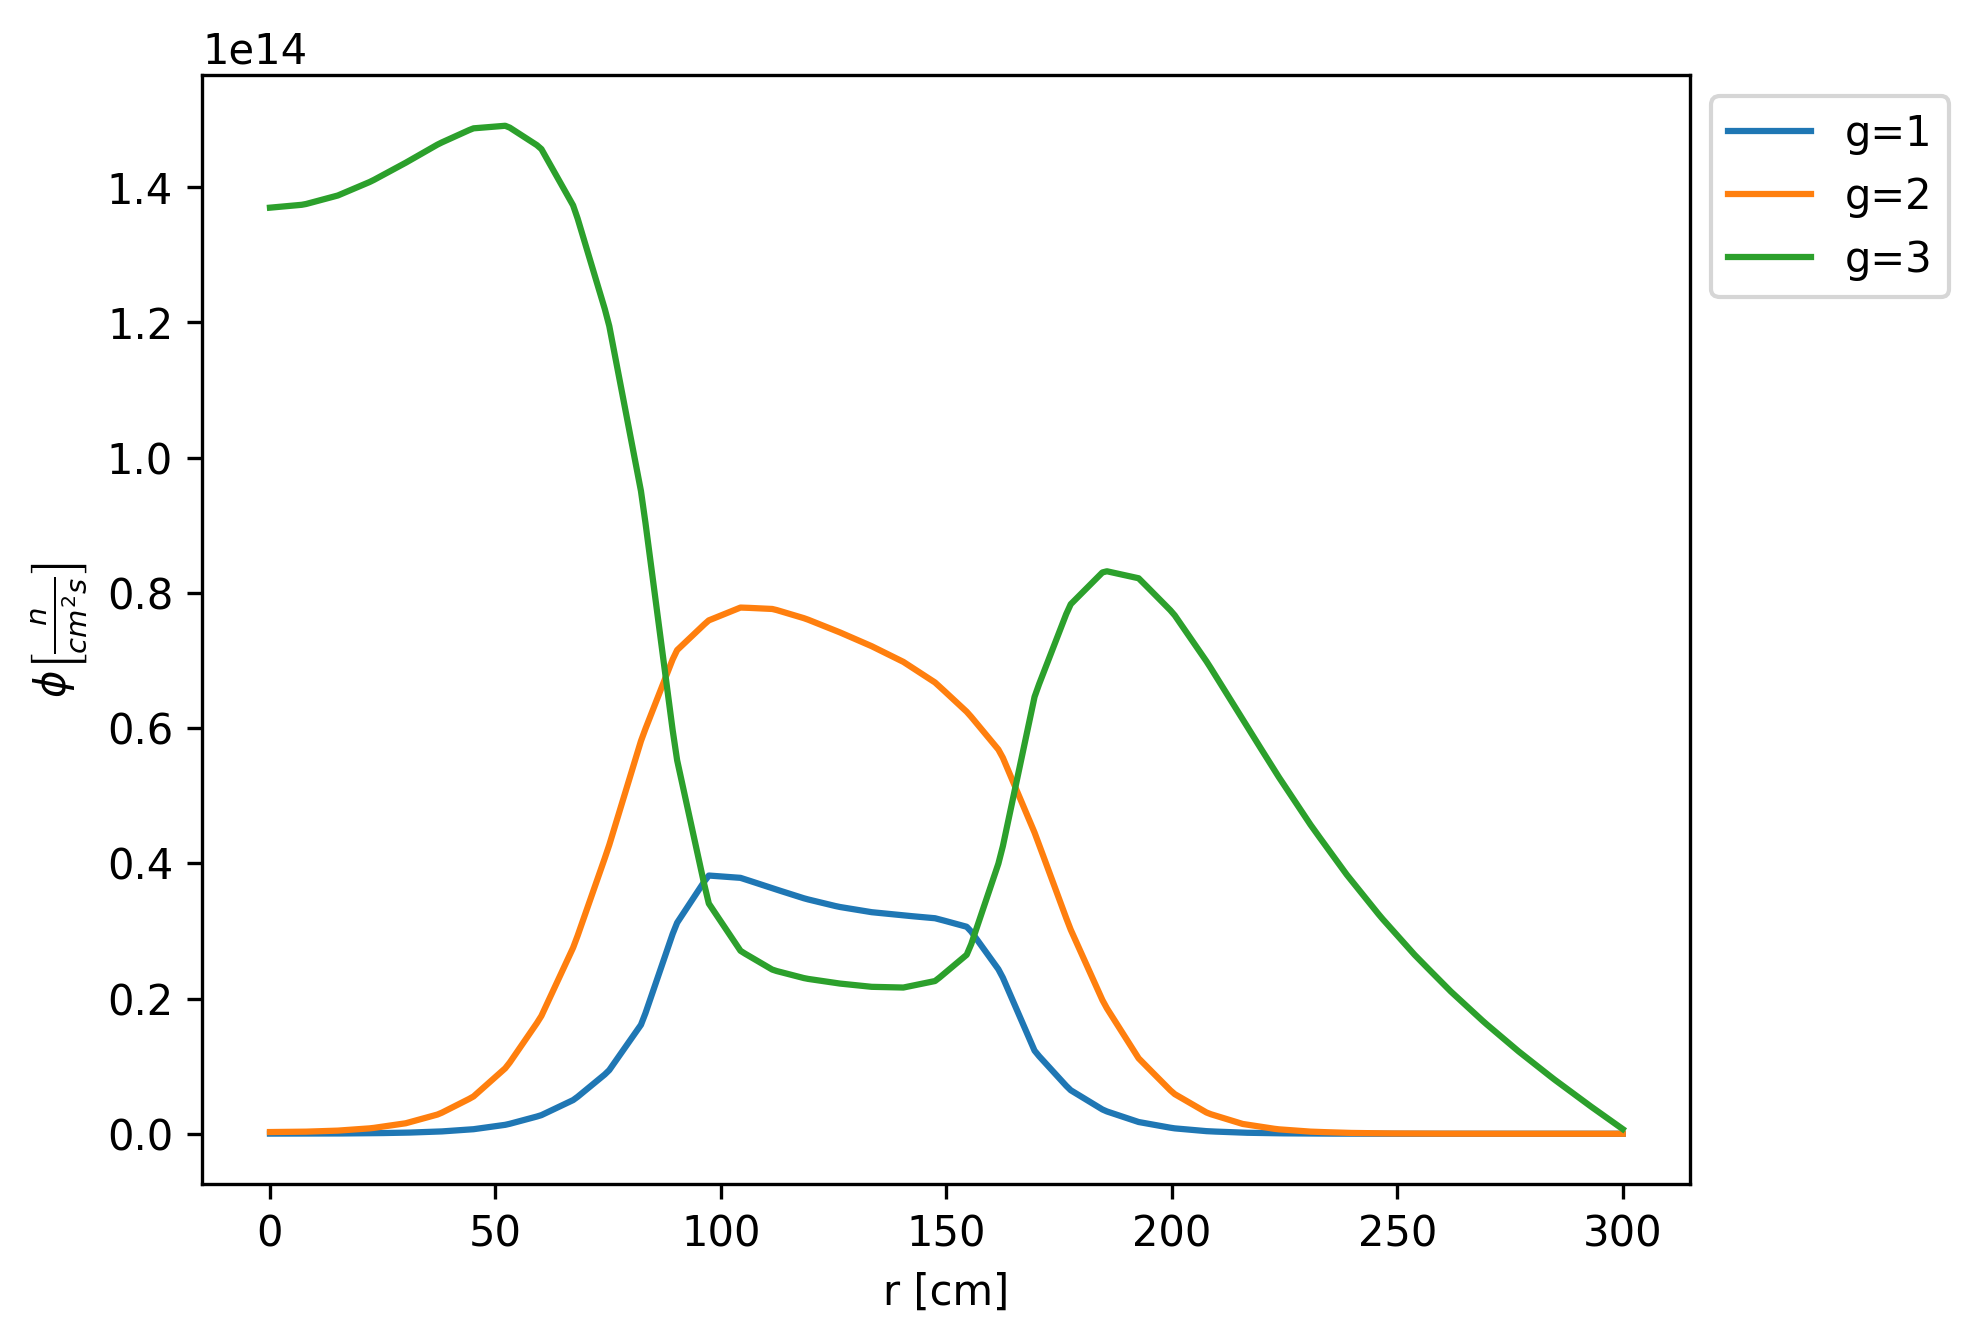
\includegraphics[width=0.45\textwidth]{figures-neutronics/3D-fullcore-600-15Gd-radial1}
    }
	\hfill
	\caption{Comparison of the radial detector flux calculated by Serpent and Moltres at 600 K.}
	\label{fig:fullcore-600-radial1}
\end{figure}

% Axial flux1 at 1200K
\begin{figure}[htbp!]
	\centering
    \subfloat[Serpent axial detector flux.]{
        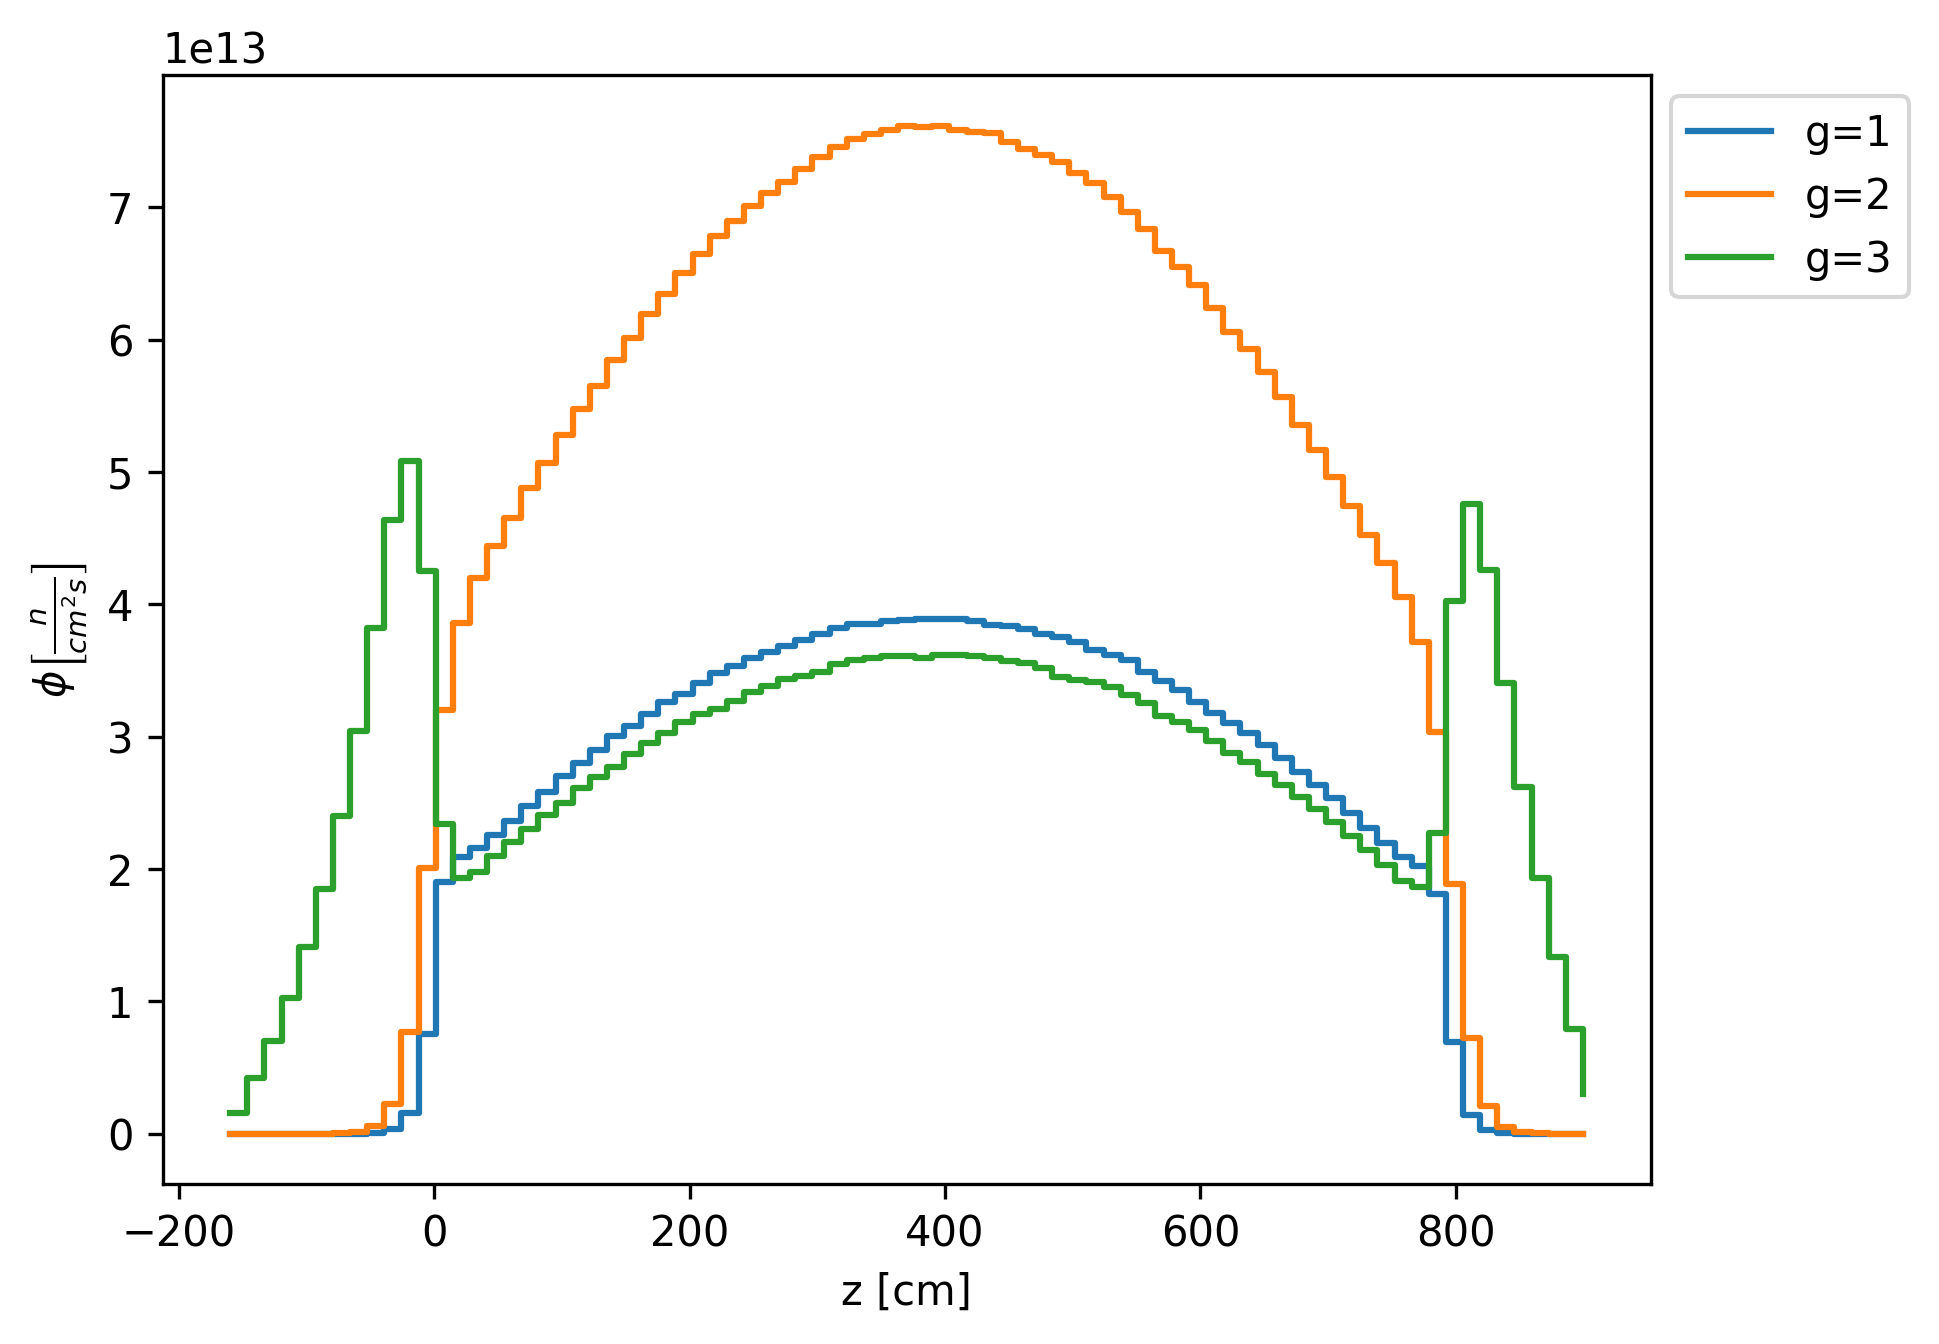
\includegraphics[width=0.45\textwidth]{figures-neutronics/serpent26G-1200-collapse-Axial1}
    }
    \subfloat[Moltres axial detector flux.]{
        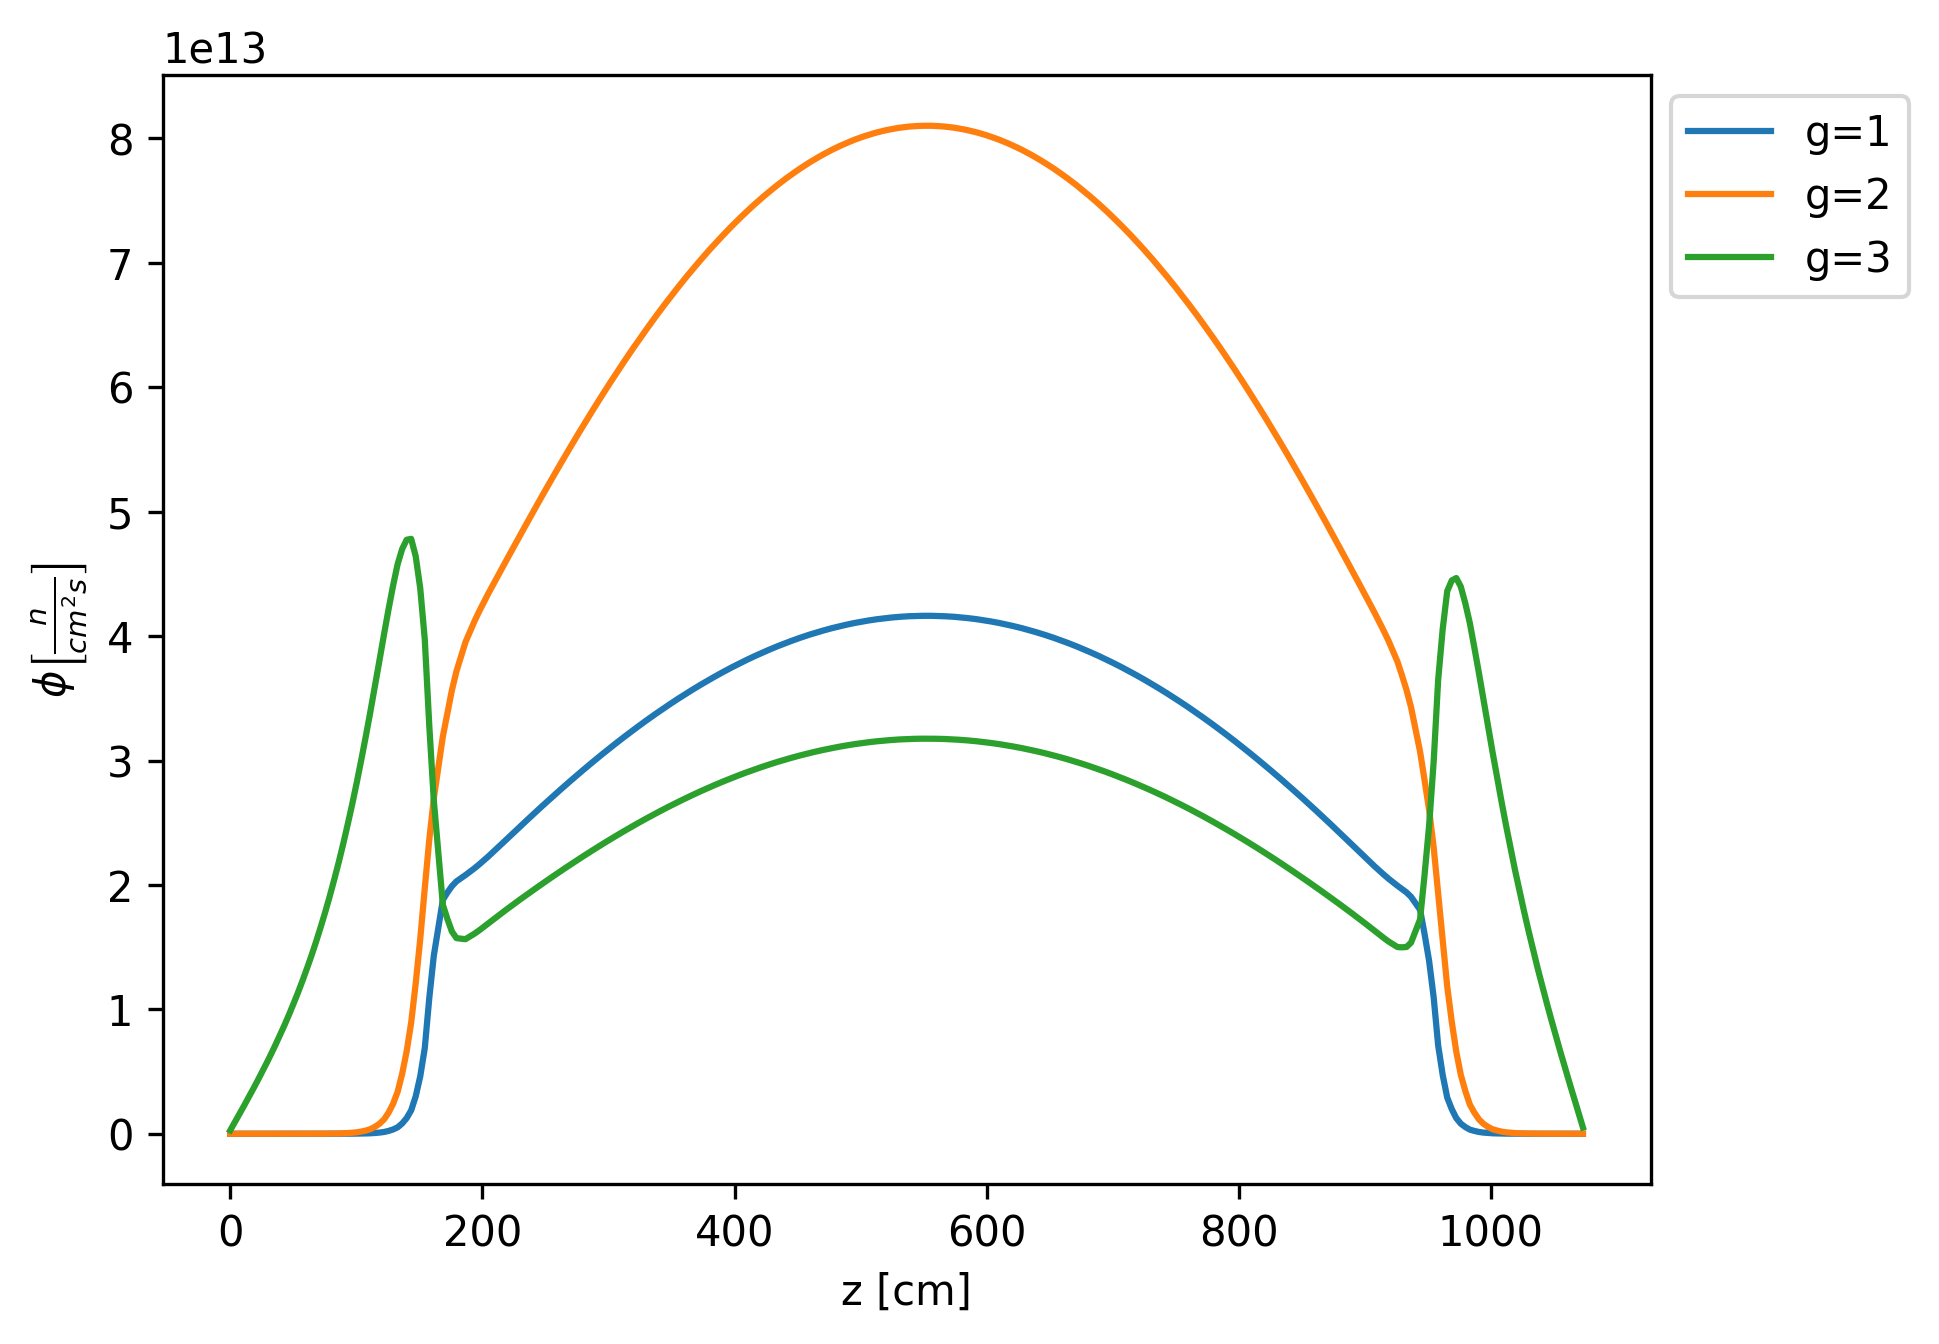
\includegraphics[width=0.45\textwidth]{figures-neutronics/3D-fullcore-1200-15Gc-axial1}
    }
	\hfill
	\caption{Comparison of the axial detector flux calculated by Serpent and Moltres at 1200 K.}
	\label{fig:fullcore-1200-axial1}
\end{figure}

%Radial flux at 1200 K
\begin{figure}[htbp!]
	\centering
    \subfloat[Serpent radial detector flux.]{
        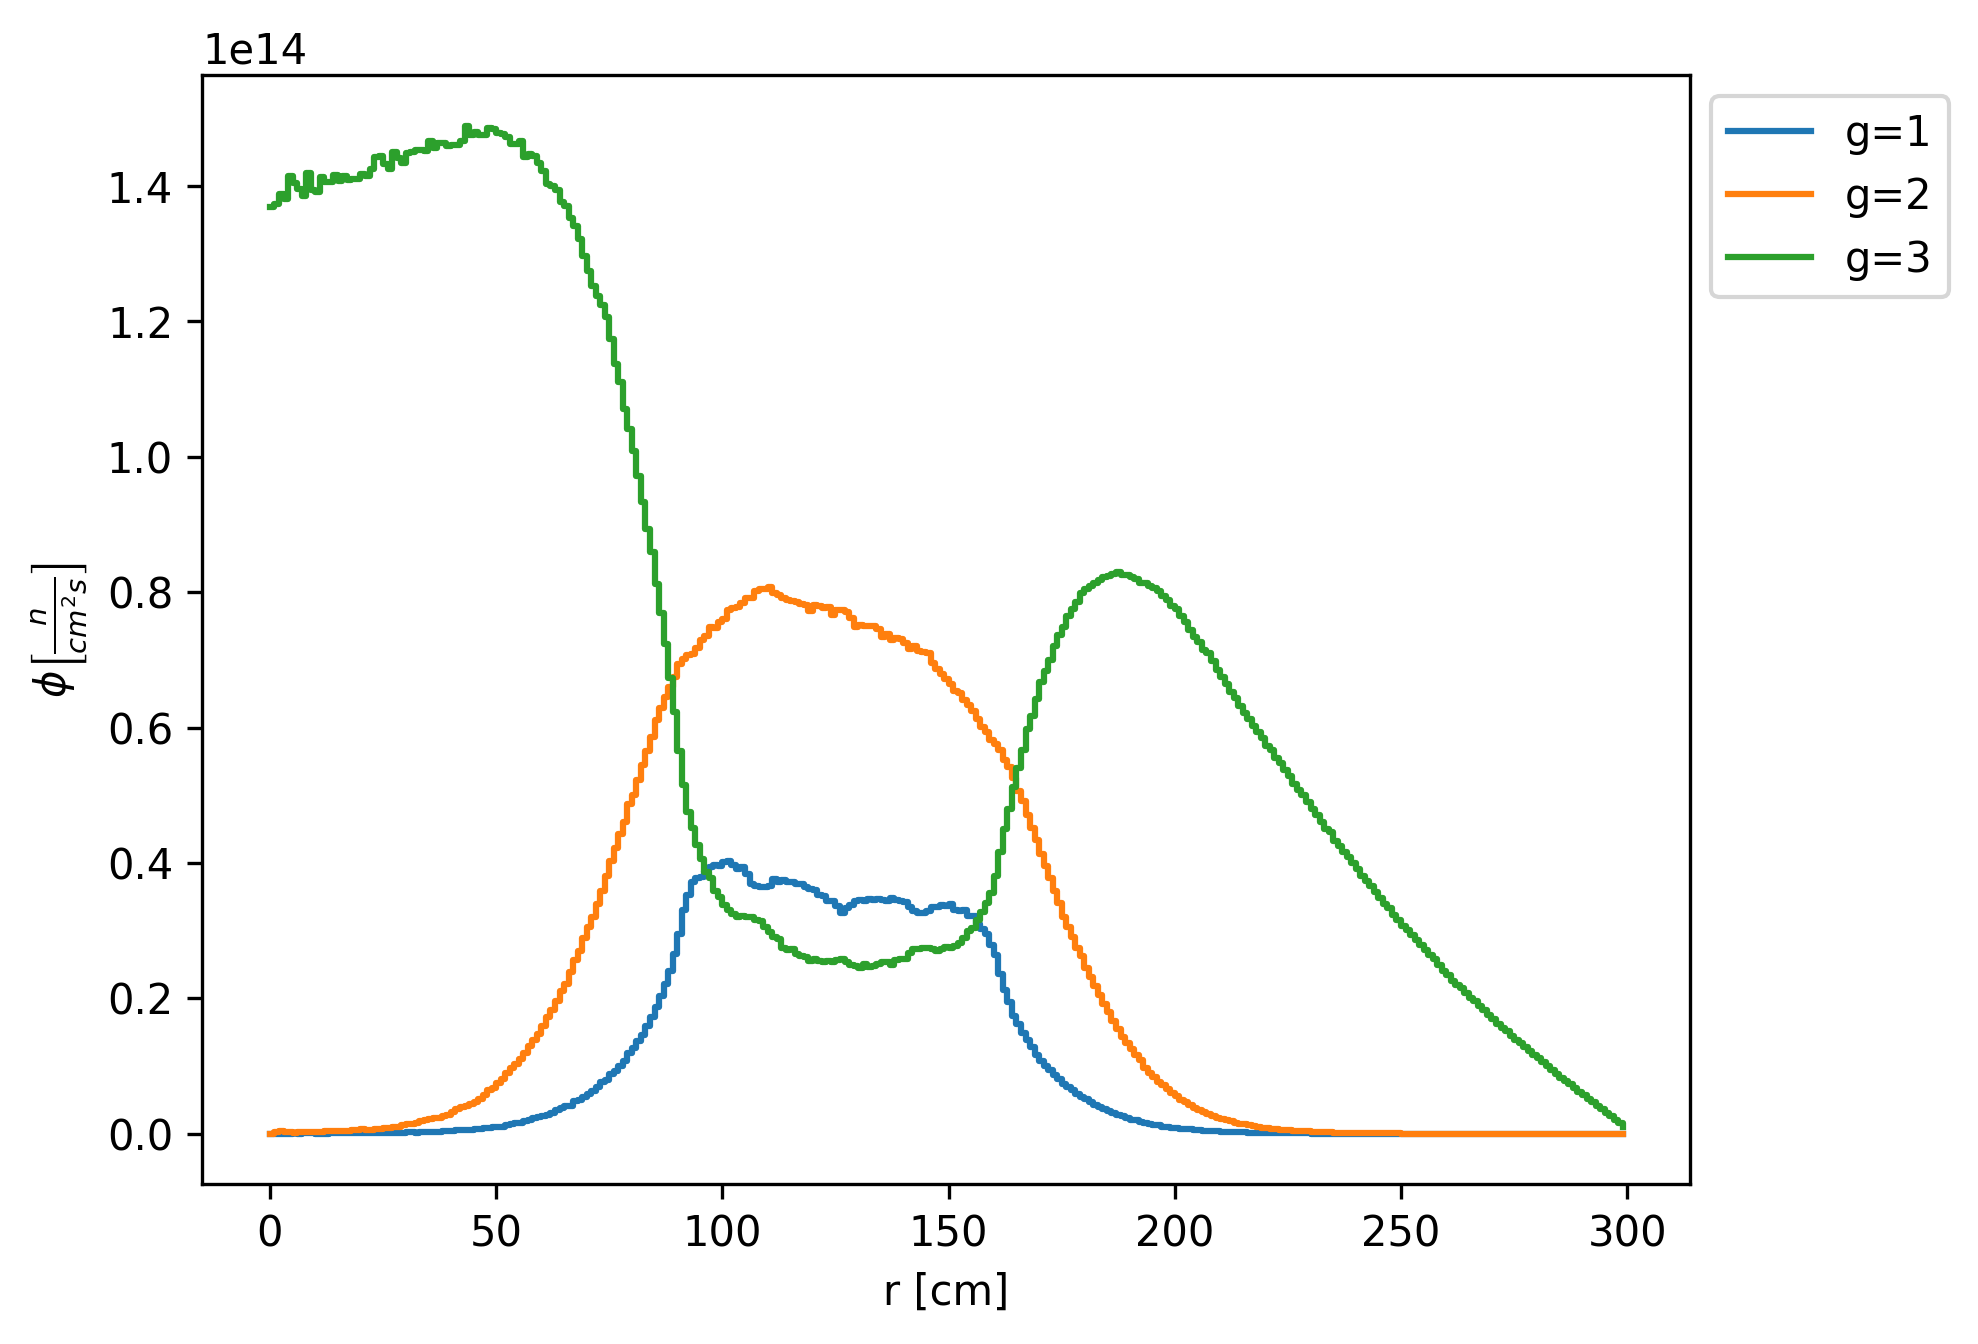
\includegraphics[width=0.45\textwidth]{figures-neutronics/serpent26G-1200-collapse-Radial}
    }
    \subfloat[Moltres radial detector flux.]{
        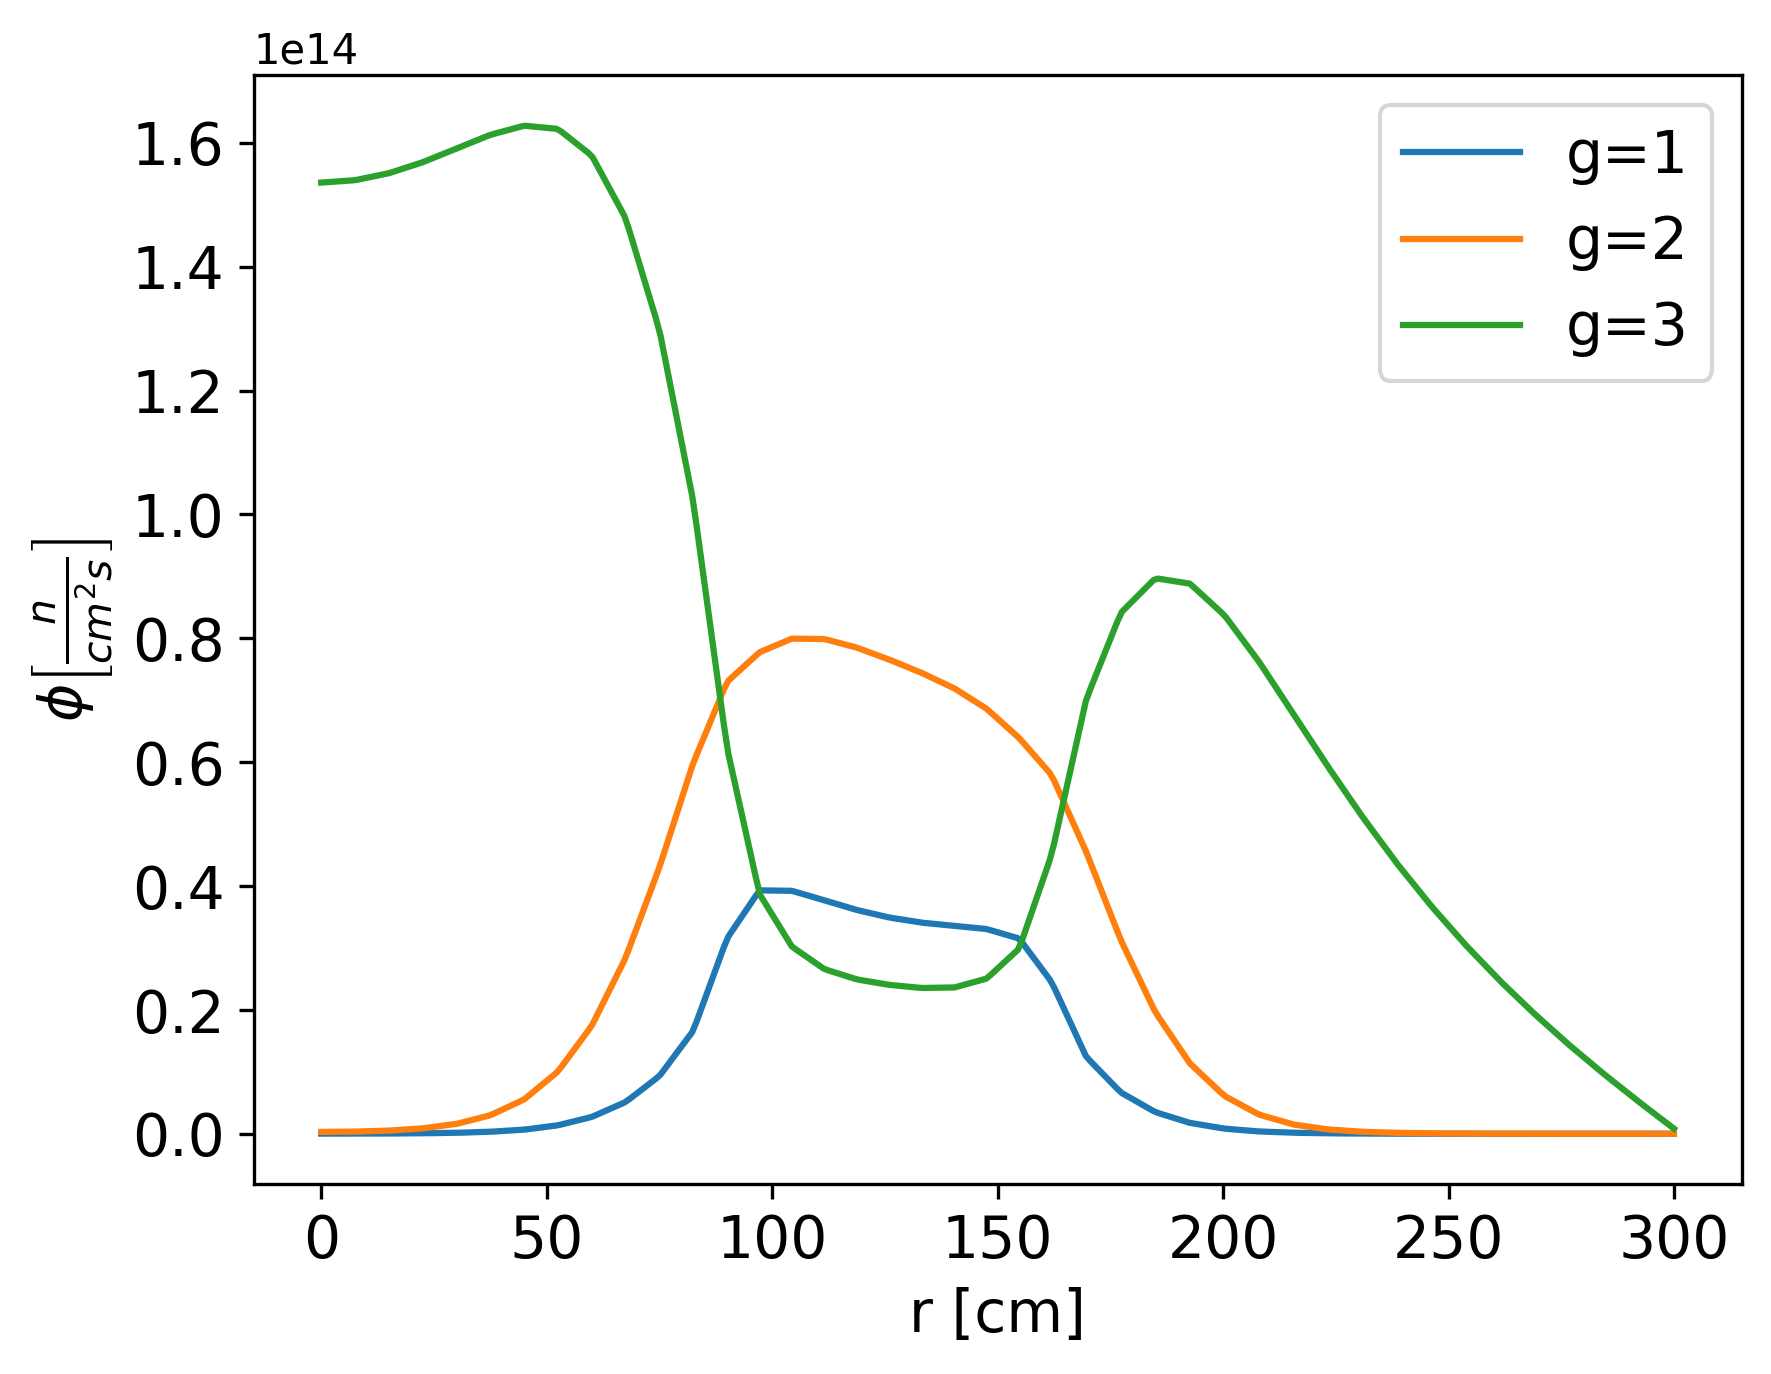
\includegraphics[width=0.45\textwidth]{figures-neutronics/3D-fullcore-1200-15Gc-radial1}
    }
	\hfill
	\caption{Comparison of the radial detector flux calculated by Serpent and Moltres at 1200 K.}
	\label{fig:fullcore-1200-radial1}
\end{figure}


\section{OECD/NEA MHTGR-350 Benchmark: Phase I Exercise 1}
\label{sec:ph1e1}

% Exercise description
This section discusses Phase I Exercise 1 of the OECD/NEA MHTGR-350 Benchmark conducted with Moltres and compares the results with those already published \cite{oecd_nea_coupled_2020}.
The benchmark specifies the group constants required to conduct the exercise, ensuring a common dataset among various benchmark participants and allowing stand-alone neutronic comparison without thermal-fluids feedback.
The exercise requests the reporting of the global parameters: $K_{eff}$, control rod worth ($\Delta \rho_{CR}$), axial offset ($AO$), and the power distribution map \cite{oecd_nea_benchmark_2017}.
Equations \ref{eq:controlrod} and \ref{eq:ao} define $\Delta \rho_{CR}$ and $AO$
\begin{align}
    \Delta \rho_{CR} &= \frac{k_{eff, out}-k_{eff, in}}{k_{eff, out}k_{eff, in}} \label{eq:controlrod}
    \intertext{where}
    \Delta \rho_{CR} &= \mbox{control rod worth} [-] \notag \\
    k_{eff, out} &= \mbox{eigenvalue with \gls{CR} out (at position z=911.7 cm)} [-] \notag \\
    k_{eff, in} &= \mbox{eigenvalue with \gls{CR} in (at position z=99 cm)} [-] \notag
		\intertext{and}
    AO &= \frac{P_{top}-P_{bottom}}{P_{top}+P_{bottom}} \label{eq:ao}
    \intertext{where}
    AO &= \mbox{axial offset } [-] \notag \\
    P_{top} &= \mbox{total power produced in the top half core } [W] \notag \\
    P_{bottom} &= \mbox{total power produced in the bottom half core } [W]. \notag
\end{align}

The Moltres simulation modeled $1/3^{rd}$ of the reactor, shown in Figure \ref{fig:bench-mesh}.
The model included the bottom and top reflectors
Two hundred and thirty-two hexagonal subdomains comprised the core, for which the benchmark provides group constants.
% Table \ref{tab:mac-region} lists the six macroscopic regions that we can differentiate in the model.
The simulations required two meshes: one for the CR out and one for the CR in.
The simulation with the CR out had 2.7 $\times 10^5$ \glspl{DoF} per energy-group, and a total of 7.0 $\times 10^6$ DoFs.
The simulation with the CR in had 2.3 $\times 10^5$ \glspl{DoF} per energy-group, and a total of 5.9 $\times 10^6$ DoFs.
The Moltres simulations obeyed an eigenvalue convergence tolerance of 1$\times$10$^{-8}$.

\begin{figure}[htbp!]
	\centering
	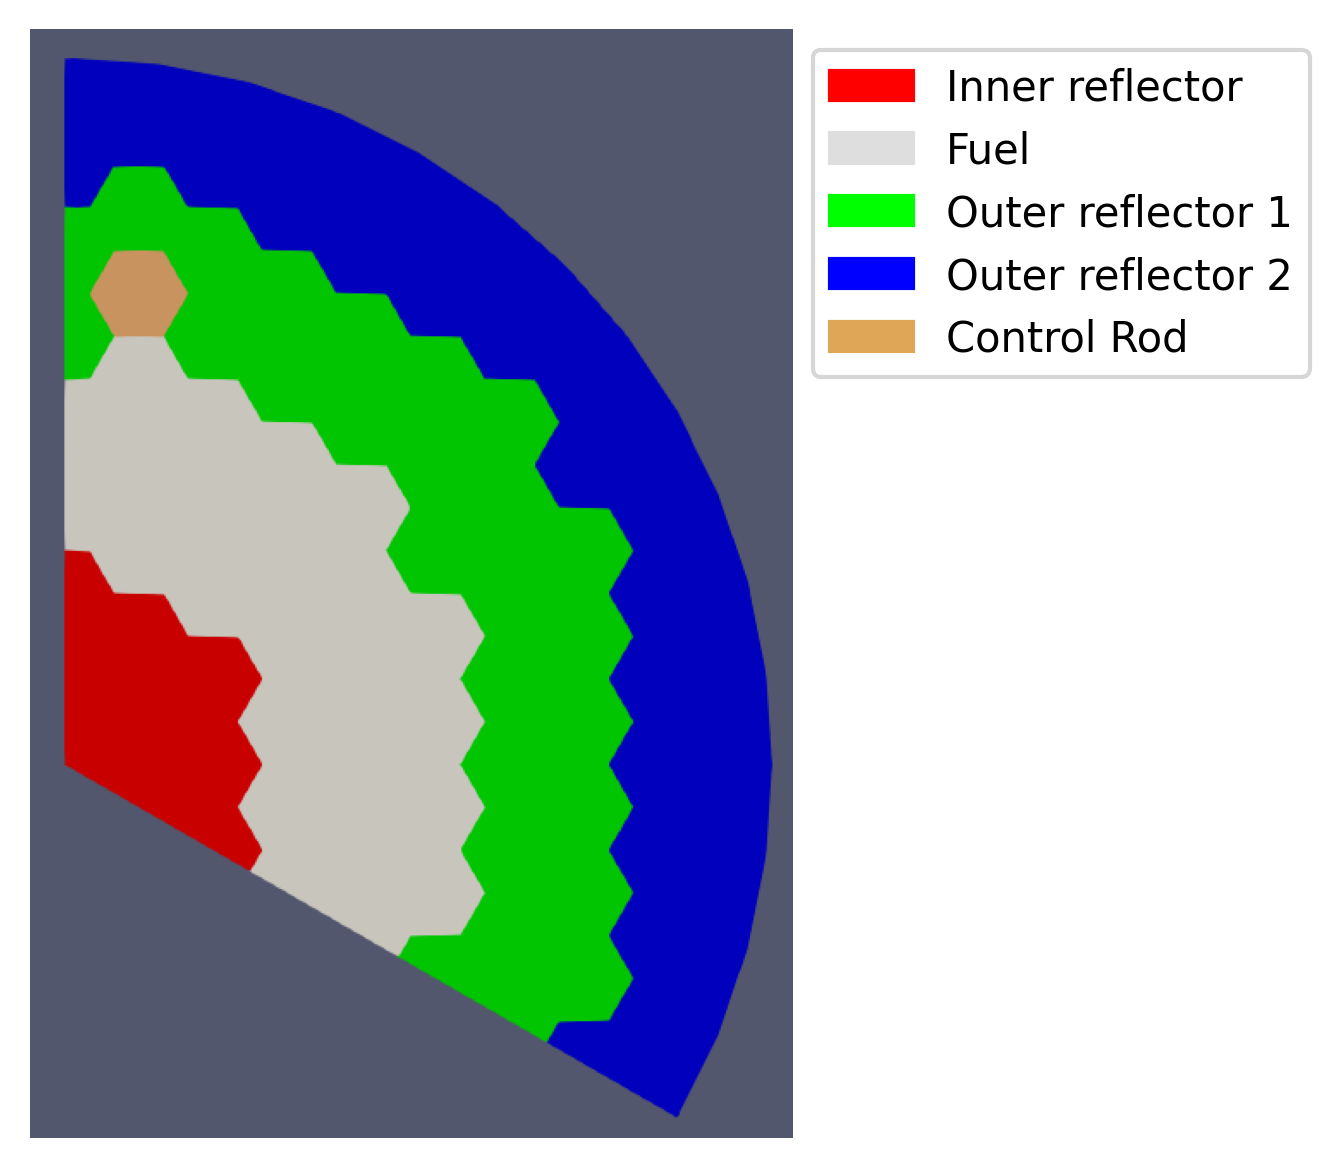
\includegraphics[width=0.55\linewidth]{figures-neutronics/oecd-fullcore-legend}
	\hfill
	\caption{Moltres model, $1/3^{rd}$ section of the MHTGR-350.}
	\label{fig:bench-mesh}
\end{figure}

% \begin{table}[htbp!]
%   \centering
%   \caption{Macroscopic regions .}
%   \label{tab:mac-region}
%   \begin{tabular}{@{}l c}
%   \toprule
%   Macroscopic region    & Subdomains     \\
%   \midrule
%   Fuel              & 1 to 220      \\
%   Bottom reflector  & 221 to 224    \\
%   Inner reflector   & 225           \\
%   Outer reflector   & 226-227       \\
%   Top reflector     & 228 to 231    \\
%   Control Rod       & 232           \\
%   \bottomrule
%   \end{tabular}
% \end{table}

The benchmark exercise specifies the group constants and a map with their location.
The benchmark definition used DRAGON-4 \cite{marleau_user_2016} to obtain the group constants from a full block configuration.
The dataset contains 26 energy groups.
Because the benchmark group constant format differs from the Moltres format, I made a Python script to handle the differences as part of this thesis.
The benchmark specifies the following group constants: $\Sigma_g^t$, $D_g$, $\nu\Sigma_g^f$, $\Sigma_g^f$, $\chi_g^t$, and $\Sigma_{g'\rightarrow g}^s$ (see equation \ref{eq:diffusion-eig}).

The benchmark exercise sets periodic \glspl{BC} on the sides of the geometry; however, a memory issue did not allow for implementing those BCs in our 26-group Moltres input file.
We approximated the periodic BC with the reflective BC.
Section \ref{sec:bench-bcs} discusses further the use of periodic and reflective BCs.

% 4.33 h and 4.11 h
On average, the simulations took 4.22 hours using 1024 cores.
Table \ref{tab:globalparam} shows the main results.
These include: Moltres predicting a \gls{Keff} larger than the reference result, a reactivity disparity of 99 pcm, Moltres yielding a smaller control rod worth (difference being 312 pcm), and the axial offset for the Moltres simulation being 4$\%$ higher than the reference result.
We attribute the discrepancies to the use of the reflective BCs instead of the periodic BCs.
Once again, Section \ref{sec:bench-bcs} discusses further the use of periodic and reflective BCs.

\begin{table}[htbp!]
  \centering
  \caption{Global parameters.}
  \begin{tabular}{lcc}
  \toprule
  Parameter 	&  Benchmark  &  Moltres    \\
  \midrule
  k$_{eff, out}$ 	&  1.06691    &  1.06804    \\
  $\Delta \rho_{CR}$ [pcm]  & 822.1 	& 509.8 \\
  AO        	&  0.168      &  0.1753     \\
  \bottomrule
  \end{tabular}
  \label{tab:globalparam}
\end{table}

Figure \ref{fig:axialpower} shows the radially averaged axial power distribution.
Figure \ref{fig:radialpower} shows the axially averaged radial power distribution.
In both figures, Moltres' values are similar to the reference results.
Moltres' power distribution in the inner ring is larger.
The differences are within 0.25 W/cm$^3$.

\begin{figure}[htbp!]
	\centering
    \subfloat[Moltres result.]{
        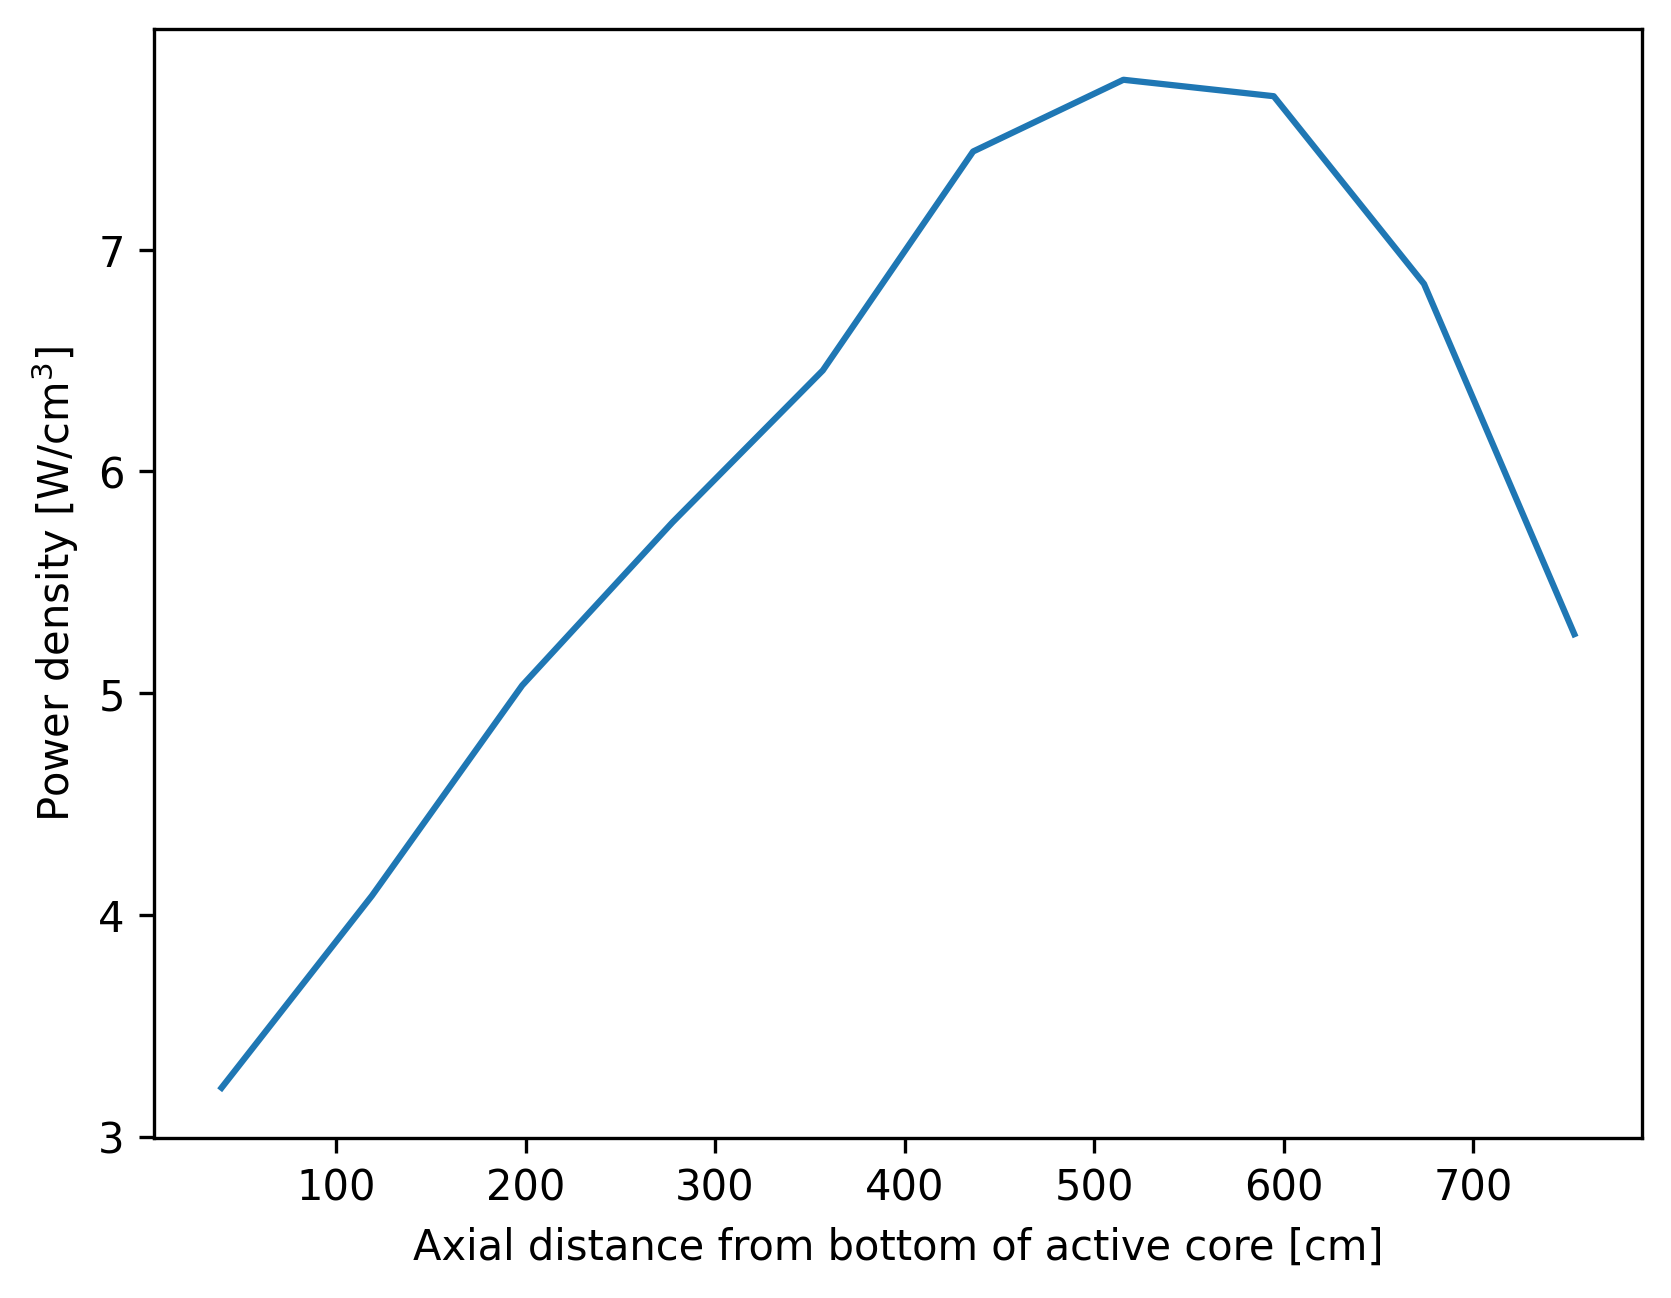
\includegraphics[width=0.42\textwidth]{figures-neutronics/3D-fullcore26G-axialpower}
    }
    \subfloat[Benchmark result. Image reproduced from \cite{oecd_nea_coupled_2020}.]{
        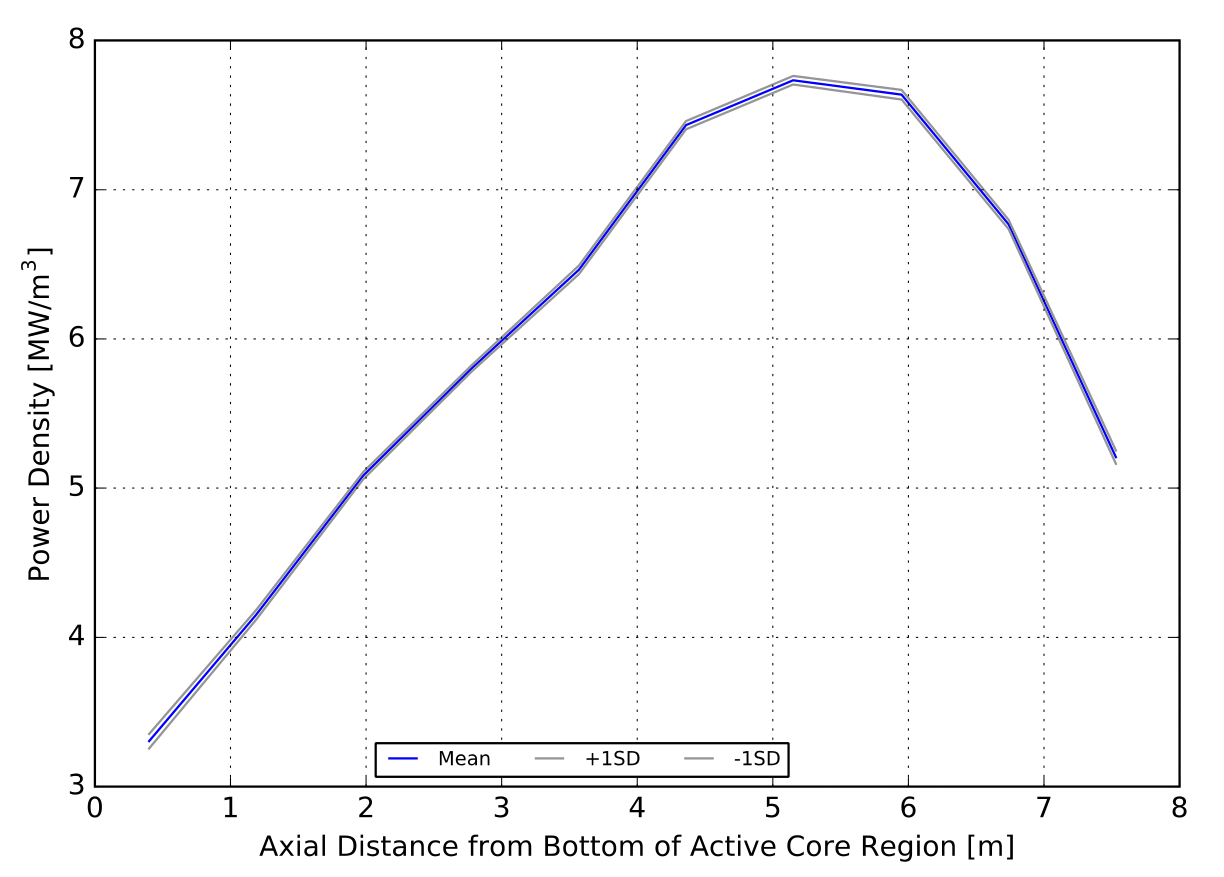
\includegraphics[width=0.47\textwidth]{figures-neutronics/benchmark-axialpower}
    }
	\hfill
	\caption{Comparison between the radially averaged axial power distribution calculated by Moltres and the benchmark published result \cite{oecd_nea_coupled_2020}.}
	\label{fig:axialpower}
\end{figure}

\begin{figure}[htbp!]
	\centering
    \subfloat[Moltres result.]{
        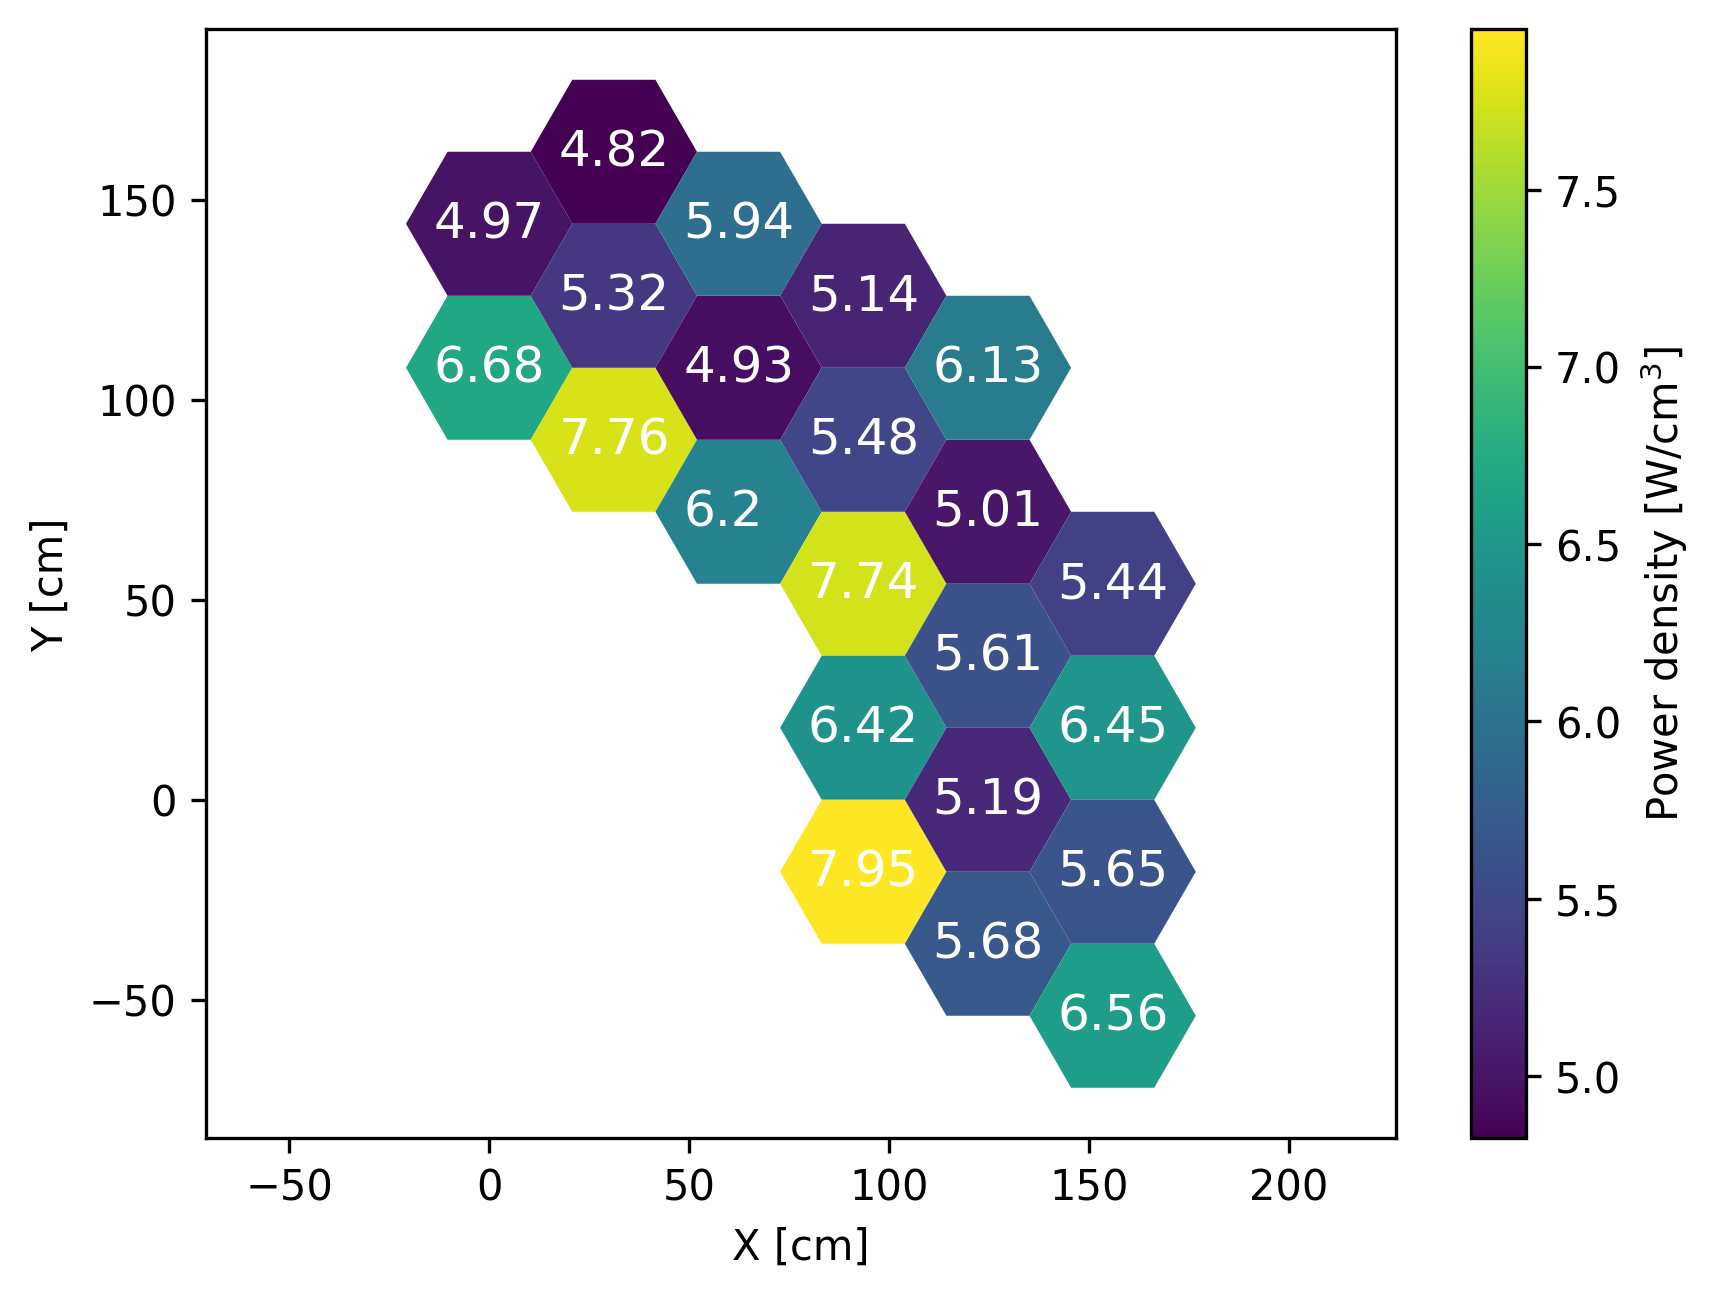
\includegraphics[width=0.47\textwidth]{figures-neutronics/3D-fullcore26G-radialpower}
    }
    \subfloat[Benchmark result. Image reproduced from \cite{oecd_nea_coupled_2020}.]{
        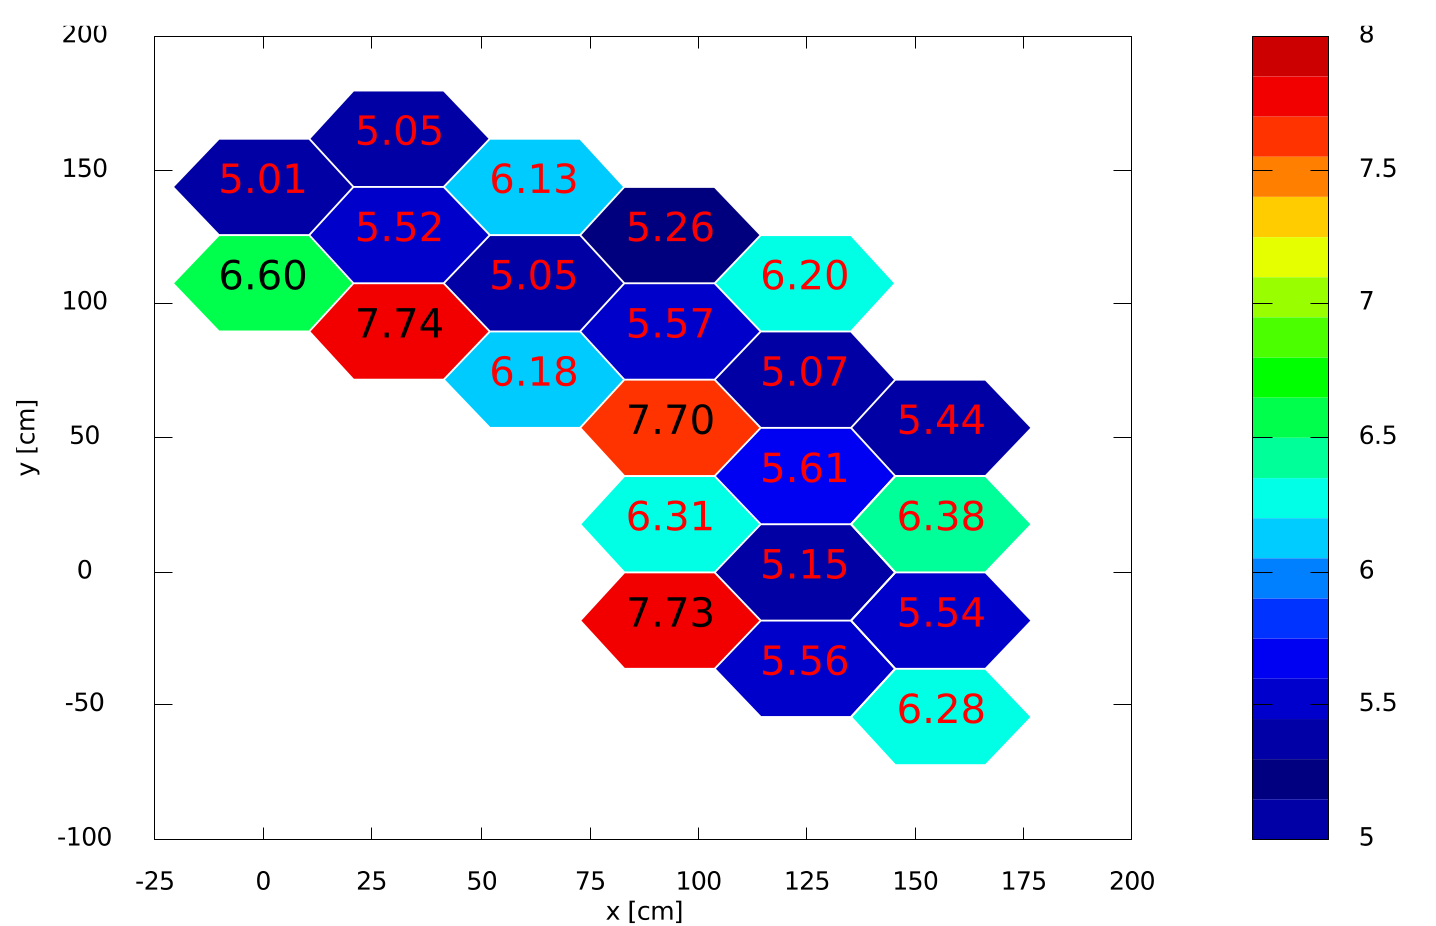
\includegraphics[width=0.42\textwidth, height=6.2cm]{figures-neutronics/benchmark-radialpower}
    }
	\hfill
  \caption{Comparison between the axially averaged radial power distribution calculated by Moltres and the benchmark published result \cite{oecd_nea_coupled_2020}.}
  \label{fig:radialpower}
\end{figure}

\subsection{Periodic vs Reflective Boundary Conditions}
\label{sec:bench-bcs}

In the last section, we observed deviations in Moltres results.
This section will analyze the discrepancies that the reflective \gls{BC} approximation may have introduced.
As the previous section mentioned, the simulation's memory requirements restrict the use of periodic BCs.
To reduce the memory requirements, we collapsed the group constants to a smaller number of energy groups.
We simulated two cases: one that uses a 3-group structure and one that uses a 6-group structure (see Table \ref{tab:energygroups}).

The simulations required two meshes each: one for the CR out and one for the CR in.
The 3-group simulation had 6.2 $\times 10^4$ DoFs per energy-group (total of 1.9 $\times 10^5$ DoFs) and 6.2 $\times 10^4$ DoFs per energy-group (total of 1.8 $\times 10^5$ DoFs) for the CR out and CR in cases, respectively.
The 6-group simulation had 1.7 $\times 10^4$ DoFs per energy-group (total of 1.0 $\times 10^5$ DoFs) and 1.9 $\times 10^4$ DoFs per energy-group (total of 1.1 $\times 10^5$ DoFs) for the CR out and CR in cases, respectively.
We highlight that the 6-group simulation had to use a coarser mesh; otherwise, it would not run.
This fact confirms the suspicion that the simulation's memory requirements prevent it from running.

We ran simulations with periodic and reflective boundary conditions for both cases and compared their results, as seen in Table \ref{tab:benchmark-bc}.
k$_{eff}$ rises with the reflective BC.
With the CR out, the raise is small.
However, with the CR in, the increase is considerable.
The combined effect of both increases leads to a decrease in the control rod worth.
The BC approximation barely affects the axial offset.

\begin{table}[htbp!]
  \centering
  \caption{Global parameter comparison for different types of BCs.}
  \begin{tabular}{clcccc}
  \toprule
  Energy groups       & Type of BCs & k$_{eff, out}$ & k$_{eff, in}$ & $\Delta \rho_{CR}$ [pcm] & AO \\
  \midrule
  \multirow{2}{*}{3}  & Periodic     & 1.07571		& 1.06776		& 692.6		& 0.237		\\
                      & Reflective   & 1.07586	  & 1.07021   & 490.5		& 0.237	  \\ \hline
  \multirow{2}{*}{6}  & Periodic     & 1.07182		& 1.06356		& 724.3	  & 0.185  	\\
                      & Reflective   & 1.07197   	& 1.06610 	& 513.3		& 0.186		\\  
  \bottomrule
  \end{tabular}
  \label{tab:benchmark-bc}
\end{table}

\section{Conclusions}
\label{sec:neutr-conc}

% Preliminary studies: homogeneous vs heterogeneous isotopic distribution
The preliminary studies focused on several aspects of the simulations.
The first aspect was the effect of distributing the fuel compact isotopes homogeneously in the Serpent model.
The results showed that the homogenization of the fuel compact isotopes decreased the multiplication factor considerably, and that the heterogeneous calculation took 28$\%$ longer.
Additionally, the homogeneous distribution appeared not to have a substantial impact on the group constants.
However, the multiplication factor's considerable difference suggested that the combined effect of the group constants’ small variations was significant.
Although explicit modeling of the TRISO particles is time-consuming, it is necessary.

% Preliminary studies: homogeneous vs heterogeneous diffusion simulation
The next section studied the problem set-up in Moltres.
Moltres uses a heterogeneous diffusion solver, making it applicable to reactor technologies that allow for heterogeneous diffusion calculations.
In this work, we aimed to use Moltres to solve prismatic HTGRs.
Nevertheless, the diffusion approximation fails to properly model regions where the mean free path is comparable to the region's dimensions.
The presence of helium in the prismatic HTGR fuel assembly challenges some of the diffusion theory assumptions.
Based on this discussion, we adapted the input group constants to carry out a homogeneous diffusion calculation using Moltres.

% Serpent-Moltres: Fuel column
Focusing on a fuel column of the MHTGR-350, we investigated the effects of the energy group structure on the diffusion calculations.
We considered four operational cases: a fuel column without burnable poisons and a fuel column with burnable poisons, both cases at 600K and 1200K.
Serpent obtained the homogenized group constants of the fuel column.
Then, Moltres took such constants as input along with a three-dimensional mesh defining the core geometry.
The first study compared the Moltres-derived axial flux to Serpent-derived axial flux.
Overall, the axial fluxes were close in shape and magnitude.
A different study focused on the effects of the energy group structure on the \gls{Keff}.
The number of energy groups did not affect the accuracy of the Moltres eigenvalue calculations.
We also compared the $L_2$-norm of the axial flux relative difference in the active core using various energy group structures.
For the four operational cases, increasing the number of energy groups improved the accuracy.
Additionally, we presented the simulation's computational expense for the different number of energy groups.
The simulation time and memory requirement rose by increasing the number of energy groups.
Finally, we analyzed the impact of using different 15-group structures on the $L_2$-norm of the axial flux relative error.
We chose $15d$ as the best-performing energy group structure.

% Serpent-Moltres: Full-core
Based on the fuel column analysis results, we compared Moltres full-core results with Serpent reference results.
We considered two operational cases: 600K and 1200K.
Serpent obtained the homogenized group constants of the different regions of the reactor, and again, Moltres took such constants as input along with a three-dimensional mesh.
The first analysis compared the Serpent and Moltres eigenvalues --- Moltres results were bigger, but the overall differences were less than 300 pcm.
The second analysis compared the radial power distributions from both codes.
These results showcased the symmetry of the problem.
Reducing the problem size by half, other simulations could reduce their computational expense.
For the most part, Moltres radial power distribution showed proximity to the Serpent's result.
We also compared Moltres and Serpent fluxes in two directions (axial and radial) in arbitrary core regions.
The axial fluxes showed small discrepancies, mostly in their magnitude.
The radial fluxes were close in shape and magnitude; however, the radial flux in the diffusion calculation failed to capture the flux variation near the burnable poisons.
Overall, the fluxes were similar.

% OECD-Benchmark
The simulation capabilities for prismatic HTGRs have not reached state of the art of LWRs.
This development delay motivated OECD/NEA to define a benchmark, which uses the MHTGR-350 as the reference design, to carry out code-to-code comparisons.
We conducted Phase I Exercise 1 with Moltres, using the group constants defined by the benchmark.
The group constants have a 26-energy group structure, and the exercise sets periodic \glspl{BC} on the sides of the geometry.
The simulation's high memory requirements have challenged such implementation in Moltres.
To circumvent this, we approximated the periodic \gls{BC} with a reflective BC.
Two out of three global parameters exhibited good agreement with the reference results; however, the control rod worth presented a large discrepancy, a consequence of the BC approximation.
Reducing the problem's size by collapsing the group constants to 3 and 6-energy groups, we compared the \gls{Keff} using the periodic and reflective BCs.
A reflective BC for the \gls{CR} out case did not substantially impact the \gls{Keff}, but the BC choice for the CR in case had a significant effect.
The combined effect of the approximation led to a large error in the CR worth, while it had only a small influence on the axial offset.

\chapter{Thermal-fluids}
\section{Preliminary studies}

This section carries out some preliminary studies using Moltres and MOOSE heat conduction module to solve the prismatic HTGR thermal-fluids.

\subsection{Verification of the thermal-fluids model}

To verify our methodology, this section solved a simplified cylindrical model whose analytical solution we know.
The model assumes a sinusoidal power profile in the $z$-direction.
Section \ref{appendix:ver} presents the analytical solution of the problem.
Moltres/MOOSE obtained the numerical solution of equations in Section \ref{ch3:th}.

Figure \ref{fig:th-ver-mesh} displays the model geometry.
The model differentiates 5 subregions: fuel compact, helium gap, moderator, film, and coolant.
Table \ref{tab:th-ver-char} summarizes the geometry dimensions and the input parameters.
Data for a VHTR based on the GT-MHR.
The moderator thickness is the VHTR unit cell minimum distance between fuel and coolant channels.
We calculated the coolant radius by preserving the coolant channel volume.

\begin{table}[htbp!]
\centering
      \caption{characteristics.}
      \label{tab:th-ver-char}
    \begin{tabular}{@{}l c S[table-format=2.2] c c}
    \toprule
    \multicolumn{1}{c}{Parameter} & multicolumn{1}{c}{Symbol} & \multicolumn{1}{c@{}}{Value} & \multicolumn{1}{c@{}}{Units} & multicolumn{1}{c}{Reference} \\
    \midrule
  Average power density & q$_{ave}$ & 35      & W/cm$^3$ & \cite{in_three-dimensional_2006} \\
  Fuel compact radius   & R$_f$     & 0.6225  & cm       & \cite{in_three-dimensional_2006} \\
  Fuel channel radius   & R$_g$     & 0.6350  & cm       & \cite{in_three-dimensional_2006} \\

  Coolant channel radius    & - 	& 0.7950  & cm       & \cite{in_three-dimensional_2006} \\
  Calculated coolant radius & R$_c$ & 0.6350  & cm       & - \\
  % material properties from \cite{tak_numerical_2008}
  \bottomrule
  \end{tabular}
\end{table}



Figure \ref{fig:th-ver-results} shows the axial and radial temperature profiles.
Both analytical and numerical solutions exhibit good agreement.
The outlet coolant temperature is 770.2 $^{\circ}$C whereas the average outlet coolant temperature of the VHTR is 950 $^{\circ}$C.
Note that this is a simplified model only for verification purposes, and it considers only one fuel channel while in the GT-MHR unit cell two fuel channels deposit their heat in one coolant channel.

\begin{figure}[htbp!]
	\centering
	\includegraphics[width=0.3\linewidth]{figures-thermal/2D-preliminar-mesh2}
	\hfill
	\caption{Scaled-down version of the model geometry.}
	\label{fig:th-ver-mesh}
\end{figure}

\begin{figure}[htbp!]
	\centering
    \subfloat[Fuel centerline and bulk coolant axial temperatures. \label{fig:th-ver-results-a}]{
        \includegraphics[width=0.45\textwidth]{figures-thermal/2D-preliminar-axial}
    }
    \subfloat[Radial temperature at z=396.5 cm.]{
        \includegraphics[width=0.45\textwidth]{figures-thermal/2D-preliminar-radial}
    }
	\hfill
    \caption{Temperature profiles.}
	\label{fig:th-ver-results}
\end{figure}

\section{Unit cell problem}

This section will solve the unit cell problem in the hot spot of an HTGR.
Intends to reproduce \cite{in_three-dimensional_2006}.
Missing material properties come from \cite{tak_numerical_2008}.
The material properties vary with the temperature (both in In et al and my simulation).


\begin{table}[htbp!]
\centering
      \caption{characteristics.}
      \label{tab:th-ver-char}
    \begin{tabular}{@{}l c S[table-format=2.2] c c}
    \toprule
    \multicolumn{1}{c}{Parameter} & multicolumn{1}{c}{Symbol} & \multicolumn{1}{c@{}}{Value} & \multicolumn{1}{c@{}}{Units} & multicolumn{1}{c}{Reference} \\
    \midrule
  Fuel compact radius       & R$_f$ & 0.6225    & cm   & \cite{in_three-dimensional_2006} \\
  Fuel channel radius       & R$_g$ & 0.6350    & cm   & \cite{in_three-dimensional_2006} \\
  Coolant film radius       & R$_i$ & 0.7950    & cm   & \cite{in_three-dimensional_2006} \\
  Coolant channel radius    & R$_c$ & 0.7950    & cm   & \cite{in_three-dimensional_2006} \\
  Fuel/coolant pitch        & p     & 1.885     & cm   & \cite{in_three-dimensional_2006} \\
  Fuel column height        & L     & 793       & cm   & \cite{in_three-dimensional_2006} \\
  % input parameter characteristics
  Average power density     & q$_{ave}$ & 35    & W/cm$^3$   & \cite{in_three-dimensional_2006} \\
  Inlet coolant temperature & T$_{in}$  & 400   & $^{\circ}$C  & \cite{in_three-dimensional_2006} \\
  Coolant channel mass flow rate & $\dot{m}$ & 0.0176 & kg/s & \cite{in_three-dimensional_2006} \\
  Helium inlet pressure & P & 70 & bar & \cite{in_three-dimensional_2006} \\
  Helium density        & \rho  & 4.94 $\times 10^{-6}$ & kg/cm$^3$ & \cite{nist} \\
  Helium heat capacity  & c$_p$ & 5188 & J/kg/K & \cite{nist} \\
  Film thermal conductivity & k_$i$ & 0.001731 & W/cm/K & - \\
  \bottomrule
  \end{tabular}
\end{table}

\begin{table}[htbp!]
  \centering
  \caption{Material properties.}
  \begin{tabular}{llll}
  \toprule
  Parameter                  & Symbol & 400$^{\circ}$C & 400$^{\circ}$C \\
  \midrule
  Fuel compact thermal conductivity & k_f & 
  Helium gap thermal conductivity   & k_g & 
  Moderator thermal conductivity    & k_m & 

  \bottomrule
  \end{tabular}
  \label{tab:maincharac}
\end{table}

\section{Fuel assembly}

This section will calculate the heat profile of a fuel assembly of a HTGR.

\section{Full core}

This section will extend the methodology to a full-ore problem and it will intend to solve Exercise 2 of Phase I of the OECD/NEA MHTGR-350 Benchmark.




\section{Neutronics and Thermal-fluids Coupling}

3 options:
- Heterogeneous model
- Homogenized media and sub-channel unit cell model: how does it solve advection ?
- Porous media model




\chapter{Hydrogen Production}
\label{ch:hydro}

Two characteristics of HTGRs, high-temperature and high thermal conversion efficiency, motivated the development of this chapter.
Those two characteristics enable highly-efficient hydrogen production.
This chapter analyzes several hydrogen production processes coupled to various nuclear reactor designs.
To find the most efficient strategy, the analysis not only considers HTGRs but also other types of reactors.
This chapter comprises the following sections:
Section \ref{sec:hydro-intro} discusses several energy challenges and introduces an alternative based on nuclear reactors and a hydrogen economy,
Section \ref{sec:hydro-objectives} summarizes the specific objectives of this chapter,
Section \ref{sec:hydro} outlines various hydrogen production methods and their energy requirements, 
Section \ref{sec:reactors} describes the characteristics of microreactors and \glspl{SMR},
Section \ref{sec:hydro-metho} presents the methodology followed in the calculations, 
Section \ref{sec:hydro-results} displays the results of the different analyses,
and Section \ref{sec:hydro-conc} concludes the chapter with a summary and the main points of the chapter.

\section{Introduction}
\label{sec:hydro-intro}

% The energy problem
Energy is one of the most vital contributors to economic growth.
In the future, economies and populations will continue to expand, and their energy demand will accompany such change \cite{burke_impact_2018} \cite{el-shafie_hydrogen_2019}.
Meeting these future needs requires the development of clean energy sources to ease the increasing environmental concerns.
As seen in Figure \ref{fig:ghg}, electricity generation was one of the economic sectors that released the most \glspl{GHG} in the \gls{US} in 2017.
As \gls{CO2} is the main component in \glspl{GHG}, decarbonizing electricity generation will allow us to meet the increases in energy demand and address the environmental concerns simultaneously.

\begin{figure}[htbp!]
	\centering
	\includegraphics[width=0.4\linewidth]{figures-hydro/total-ghg-2017.png}
	\hfill
	\caption{Total US GHG emissions by economic sector in 2017. Image reproduced from \cite{us_epa_sources_2020}.}
	\label{fig:ghg}
\end{figure}

% word on solar energy and the duck curve
To address these concerns, utility companies rely more and more on renewable energy resources, such as wind and solar \cite{ming_resource_2019}.
However, high solar adoption creates a challenge.
The need for electricity generators to ramp up quickly increases when the sun sets and the contribution from the photovoltaics falls \cite{us_department_of_energy_confronting_2017}.
The "duck curve" (or duck chart) in Figure \ref{fig:duck} depicts this phenomenon.
The \gls{CAISO} developed the duck curve to illustrate the grid's net load \cite{bouillon_prepared_2014}.
This thesis defines the net load as the difference between the forecasted load and expected electricity production from solar.

Moreover, the duck curve reveals another issue.
Over-generation may occur during the middle of the day, and high-levels of non-dispatchable generation may exacerbate the situation.
Consequently, the market would experience sustained zero or negative prices during the middle of the operating day \cite{bouillon_prepared_2014}.

\begin{figure}[htbp!]
	\centering
	\includegraphics[width=0.75\linewidth]{figures-hydro/caiso-duck.png}
	\hfill
	\caption{The duck curve. The $x$-axis represents the hours of the day. Image reproduced from \cite{bouillon_prepared_2014}.}
	\label{fig:duck}
\end{figure}

% solutions to the duck curve
The simplest solution to a demand ramp-up is to increase dispatchable generation, which uses resources with fast ramping and fast starting capabilities such as natural gas and coal \cite{bouillon_prepared_2014}, consequently decreasing non-dispatchable generation, such as geothermal, nuclear, and hydro.
Nonetheless, an approach like this is inconsistent with the goal of reducing carbon emissions.
Hence, our focus drifts to other potential low-carbon solutions, like nuclear generation and energy storage through \gls{H2} production.

% Transportation problem
Unfortunately, a carbon-neutral electric grid will be insufficient to halt climate change because transportation is a significant contributor to \gls{GHG} emissions.
As seen in Figure \ref{fig:ghg}, transportation released the most \glspl{GHG} in the \gls{US} in 2017. Thus, decarbonizing transportation underpins global carbon reduction.
One possible strategy is to develop a hydrogen economy, as Japan is currently doing.
Japan's strategy rests on the firm belief that \gls{H2} can be a decisive response to its energy and climate challenges.
It could foster deep decarbonization of the transport, power, industry, and residential sectors while strengthening energy security \cite{nagashima_japans_2018}.
In the transportation sector, Japan plans to deploy fuel cell vehicles, trucks, buses, trains, and ships.
Although \gls{H2} technologies release zero CO$_2$, any \gls{H2} production method is only as carbon-free as the energy source it relies on (electric, heat, or both).
Nuclear reactors introduce a clean energy option to manufacture \gls{H2}.

\gls{UIUC} is leading by example and actively working to reduce \gls{GHG} emissions from electricity generation and transportation (among other sectors) on its campus.
In pursuance of those efforts, the university developed the \gls{icap}.

% ICAPP
In 2008, \gls{UIUC} signed the American College and University Presidents' Climate Commitment, formally committing to becoming carbon neutral as soon as possible, no later than 2050.
The university developed the \gls{icap} in 2010 as a comprehensive roadmap toward a sustainable campus environment \cite{isee_illinois_2015}.
The \gls{icap} defines a list of goals, objectives, and potential strategies for several topical areas, including electricity generation and transportation.

\section{Objectives}
\label{sec:hydro-objectives}

This chapter focuses on two areas: transportation and electricity generation on the \gls{UIUC} campus.
Consequently, this work's objective aligns with the efforts in two of the six target areas defined on the \gls{icap}.

Regarding transportation, the objective is to quantify UIUC fleet fuel consumption, determine how much \gls{H2} enables the fleet conversion to \glspl{FCEV}, and find reactor designs that meet the \gls{H2} demand.

Regarding electricity generation, the objective is to quantify the magnitude of the duck curve in the UIUC's grid, determine how much \gls{H2} a reactor coupled to a \gls{H2} production process could produce, and how much electricity that \gls{H2} would generate if converted.


\section{Hydrogen production methods}
\label{sec:hydro}

This section introduces several hydrogen production processes and their energy requirements.

\subsection{Electrolysis}

The electrolysis of water is a well-known process whose commercial use began in 1890.
This process produces approximately 4\% of \gls{H2} worldwide.
The process is ecologically clean because it does not emit \glspl{GHG}.
However, in comparison with other methods, electrolysis is a highly energy-demanding technology \cite{kalamaras_hydrogen_2013}.

Three electrolysis technologies exist.
Alkaline-based is the most common, the most developed, and the lowest in capital cost.
It has the lowest efficiency and, therefore, the highest electrical energy cost.
Proton exchange membrane electrolyzers are more efficient but more expensive than Alkaline electrolyzers.
\gls{SOEC} electrolyzers are the most electrically efficient but the least developed.
\gls{SOEC} technology has challenges with corrosion, seals, thermal cycling, and chrome migration \cite{kalamaras_hydrogen_2013}.
The first two technologies work with liquid water, and the latter requires high-temperature steam, so this work refers to the first two as \gls{LTE} and the latter as \gls{HTE}.

Water electrolysis converts electric and thermal energy into chemical energy stored in hydrogen.
The process enthalpy change $\Delta H$ determines the required energy for the electrolysis reaction to take place, in which part of the energy corresponds to electric energy $\Delta G$ and to thermal energy $T \cdot \Delta S$

\begin{align}
	\Delta H &= \Delta G + T \Delta S \label{eq:electrolysis1}
    \intertext{where}
    \Delta H &= \mbox{specific total energy } [kWh \cdot kg_{H_2}^{-1}] \notag \\
    \Delta G &= \mbox{specific electrical energy } [kWh \cdot kg_{H_2}^{-1}] \notag \\
    T \Delta S &= \mbox{specific thermal energy } [kWh \cdot kg_{H_2}^{-1}]. \notag
\end{align}

In \gls{LTE}, electricity generates the thermal energy.
Hence, $\Delta H$ alone determines the process’s required energy.
$\Delta H$ is equal to 60 kWh/kg-H$_2$ considering a 67$\%$ electrical efficiency \cite{usdrive_hydrogen_2017}.

In \gls{HTE}, a high-temperature heat source is necessary to provide the thermal energy.
$\Delta G$ decreases with increasing temperatures, as seen in Figure \ref{fig:electro1}.
Decreasing the electricity requirement results in higher overall production efficiencies since heat-engine-based electrical work has a thermal efficiency of 50$\%$ or less \cite{j_e_obrien_high_2010}.
Figure \ref{fig:electro1} shows $\Delta G$ and $T \Delta$S.
The analyses considered the \gls{SOEC}'s $\Delta G$ to have an electrical efficiency of 88$\%$ \cite{helmeth_high_2020}.
$T \Delta S$ accounts for the latent heat of water vaporization.
Note that the process is at 3.5 MPa.
Although $\Delta G$ increases with pressure, a high pressure saves energy, as compressing liquid water is cheaper than compressing H$_2$ \cite{obrien_status_2010}.

\begin{figure}[htbp!]
	\centering
	\includegraphics[width=0.6\linewidth]{figures-hydro/hte-energy-P.png}
	\hfill
	\caption{Energy required by HTE at 3.5 MPa.}
	\label{fig:electro1}
\end{figure}

Equations \ref{eq:electrolysis2a} and \ref{eq:electrolysis2b} determine the electrical $P_{EH2}$ and thermal power $P_{TH2}$ required by the hydrogen plant

\begin{align}
	P_{EH2} &= \dot{m}_{H2} \Delta G \label{eq:electrolysis2a} \\
	P_{TH2} &= \dot{m}_{H2} T \Delta S \label{eq:electrolysis2b}
	\intertext{where}
	P_{EH2} &= \mbox{total electrical power } [kW] \notag \\
	P_{TH2} &= \mbox{total thermal power } [kW] \notag \\
	\dot{m}_{H2} &= \mbox{\gls{H2} production rate } [kg \cdot h^{-1}]. \notag
\end{align}

\subsection{Sulfur-Iodine Thermochemical Cycle}

A thermochemical water-splitting process converts water into hydrogen and oxygen by a series of thermally driven chemical reactions.
The direct thermolysis of water requires temperatures above 2500 $^{\circ}$C for significant hydrogen generation.
At this temperature, the process can decompose 10\% of the water.
A thermochemical water-splitting cycle accomplishes the same overall result using much lower temperatures.

General Atomics, Sandia National Laboratories, and the University of Kentucky compared 115 cycles that would use high-temperature heat from an advanced nuclear reactor \cite{brown_high_2003}.
The report specified a set of screening criteria used to rate each cycle.
Some of the cycles' desirable characteristics were minimal chemical reactions and separation steps, a high abundance of the elements, a minimal solids flow, and good compatibility between heat input temperature and the permitted materials' high temperature.
The highest scoring method was the \gls{SI} cycle.

The \gls{SI} cycle consists of the three chemical reactions represented in Figure \ref{fig:sulfur1}.
The whole process inputs are water and high-temperature heat, having no need for electricity.
The process recycles all reagents and lacks effluents \cite{yildiz_efficiency_2006}.
The chemical reactions are
\begin{align}
	I_2 + SO_2 + 2H_2O &\rightarrow 2HI + H_2SO_4 \\
	H_2SO4 &\rightarrow SO_2 + H_2O + 1/2O_2 \\
	2HI &\rightarrow I_2 + H_2.
\end{align}

\begin{figure}[htbp!]
	\centering
	\includegraphics[width=0.5\linewidth]{figures-hydro/sulfur1.png}
	\hfill
	\caption{Diagram of the Sulfur-Iodine Thermochemical process. Image reproduced from \cite{benjamin_russ_sulfur_2009}.}
	\label{fig:sulfur1}
\end{figure}

Figure \ref{fig:sulfur2} presents the specific energy requirements of the cycle $\Delta H$.
Several sources disagree on the minimum temperature for the process to be viable.
This work considers the process feasible only for temperatures above 800 $^{\circ}$C.
Finally, equation \ref{eq:sulfur4} determines the thermal power $P_{TH2}$ required by the hydrogen plant
\begin{align}
	P_{TH2} &= \dot{m}_{H2} \Delta H \label{eq:sulfur4}
	\intertext{where}
	P_{TH2} &= \mbox{total thermal power } [kW] \notag \\
	\dot{m}_{H2} &= \mbox{\gls{H2} production rate } [kg \cdot h^{-1}] \notag \\
	\Delta H &= \mbox{specific energy } [kWh \cdot kg_{H_2}^{-1}]. \notag
\end{align}

\begin{figure}[htbp!]
	\centering
	\includegraphics[width=0.55\linewidth]{figures-hydro/si-energy2.png}
	\hfill
	\caption{Energy required by the Sulfur-Iodine Thermochemical Cycle.}
	\label{fig:sulfur2}
\end{figure}


\section{Microreactors and Small Modular Reactors}
\label{sec:reactors}

The typical \gls{UIUC}'s grid demand is smaller than 80 MW \cite{dotson_optimal_2020}.
Accordingly, the following analyses consider reactors of small capacities, such as microreactors and \glspl{SMR}.

These reactor concepts share several features.
The reactors require limited on-site preparation as their components are factory-fabricated and shipped out to the generation site.
This feature reduces up-front capital costs, enables rapid deployment, and expedites start-up times.
These reactors allow for black starts and islanding operation mode.
They can start up from an utterly de-energized state without receiving power from the grid.
They can also operate connected to the grid or independently.
Moreover, these reactors use passive safety systems, minimizing electrical parts.

Microreactors have the distinction that they are transportable.
Small designs make it easy for vendors to ship the entire reactor by truck, shipping vessel, or railcar.
These features make the technology appealing for a wide range of applications, such as deployment in remote residential locations and military bases.

The \gls{DOE} defines a microreactor as a reactor that generates from 1 to 20 MWth \cite{us-doe_ultimate_2019}.
The \gls{IAEA} describes an \gls{SMR} as a reactor whose power is under 300 MWe.
The IAEA defines, as well, a 'very small modular reactor' as a reactor that produces less than 15 MWe \cite{world_nuclear_association_small_2020}.
As the definitions of these reactor concepts overlap, this work considers reactors of less than 100 MWth regardless of their specific classification.


\section{Methodology}
\label{sec:hydro-metho}

In this analysis, the energy source (electric and thermal) is a nuclear reactor with co-generation capabilities.
The nuclear reactor supplies the grid with electricity $P_E$ while providing a hydrogen plant with electricity $P_{EH2}$ and thermal energy $P_{TH2}$, as shown in Figure \ref{fig:cogen}.

\begin{figure}[htbp!]
	\centering
	\includegraphics[height=5.0cm]{figures-hydro/hte-figure0.png}
	\hfill
	\caption{Diagram of a reactor coupled to a hydrogen plant.}
	\label{fig:cogen}
\end{figure}

$\beta$ and $\gamma$ determine the distribution of the reactor thermal power $P_{th}$ into $P_E$, $P_{EH2}$, and $P_{TH2}$

\begin{align}
	P_{E} &= \eta \beta P_{th} 	\\
	P_{EH2} &= \eta \gamma (1-\beta) P_{th} \\
	P_{TH2} &= (1-\gamma) (1-\beta) P_{th}
	\intertext{where}
    \eta &= \mbox{thermal-to-electric conversion efficiency} [-] \notag
    \intertext{giving}
	\beta &= \frac{P_{E} / \eta}{P_{E} / \eta + P_{TH2}/(1-\gamma)} \label{eq:cogen1} \\
	\gamma &= \frac{P_{EH2} / \eta}{P_{EH2} / \eta + P_{TH2}}. \label{eq:cogen2}
\end{align}

If $\beta = 1$, the reactor only supplies the grid with electricity $P_E$, and the hydrogen plant does not produce \gls{H2}.
If $\beta = 0$, the reactor only supplies the hydrogen plant, and electricity does not flow into the grid.
Table \ref{tab:cogen1} summarizes the values that $\gamma$ takes for the various methods.

\begin{table}[htbp!]
    \centering
    \caption{Energy requirements of the different \gls{H2} production methods.}
    \begin{tabular}{lccc}
    \toprule
    Method    & $\gamma$         & $P_{EH2}$ & $P_{TH2}$ \\
	\midrule
    LTE & 1                & $\ne$ 0   & 0         \\
    HTE & $0 < \gamma < 1$ & $\ne$ 0   & $\ne$ 0   \\
    SI  & 0                & 0         & $\ne$ 0   \\
    \bottomrule
    \end{tabular}
    \label{tab:cogen1}
\end{table}

This thesis focuses on two areas: transportation and electricity generation on the \gls{UIUC} campus.
Regarding transportation, Section \ref{sec:results-transport} discusses the conversion of the \gls{UIUC} fleet operating on campus to \glspl{FCEV}.
The analysis includes the conversion of the \gls{MTD} fleet as well.
The first step determines the fuel consumed by both fleets and how much \gls{H2} enables the fleets' complete conversion.
The next step evaluates several reactor designs and analyzes which ones could produce enough \gls{H2} to fulfill both fleet requirements.

Section \ref{sec:results-electric} focuses on electricity generation in UIUC's grid.
The first step in the analyses quantifies the magnitude of the duck curve in UIUC's grid.
To mitigate the consequences of over-generation, in a scenario in which a nuclear reactor is the primary source of energy, this analysis uses the over-generated energy to manufacture \gls{H2}.
The next step in the analysis quantifies how much \gls{H2} several production methods can generate.
The last step in the analysis calculates how much electricity the \gls{H2} could produce.

Both studies propose the same solution - a nuclear reactor coupled to a hydrogen plant.
In terms of electricity generation, this solution decreases the need for dispatchable sources and, consequently, reduces carbon emissions.
In terms of transportation, it eliminates carbon emissions.


\section{Results}
\label{sec:hydro-results}

This section holds the results of the transportation sector analysis, Section \ref{sec:results-transport}, and the Energy Generation analysis, Section \ref{sec:results-electric}.

\subsection{Transportation}
\label{sec:results-transport}

This section studies the transportation sector fuel requirements.
Figure \ref{fig:fuel} displays the fuel consumed per day by \gls{MTD} and \gls{UIUC} fleet.
The values shown in Table \ref{tab:equiv} allow for calculating the \gls{H2} requirement for MTD and UIUC fleets, shown in Figure \ref{fig:hydro-fleet}.
Table \ref{tab:hydro-fleet} summarizes the results.

	\begin{figure}[htbp!]
		\centering
        \subfloat[\gls{MTD} fleet. Data go from July 1, 2018, until June 30, 2019 \cite{mtd_irecords_2019}. Data was rearranged to represent a calendar year.]{
            \includegraphics[width=0.45\textwidth]{figures-hydro/mtd2}
        }
        \subfloat[\gls{UIUC} fleet. Data go from January 1, 2019, until December 31, 2019 \cite{uiuc_personnal_communication}.]{
            \includegraphics[width=0.45\textwidth]{figures-hydro/uiuc}
        }
		\hfill
		\caption{Fuel consumption data of MTD and UIUC fleet.}
		\label{fig:fuel}
	\end{figure}

	\begin{table}[htbp!]
	\centering
	\caption{H$_2$ necessary to replace a gallon of fuel \cite{doe_office_of_energy_efficiency_and_renewable_energy_hydrogen_2020} \cite{alternative_fuels_data_center_fuel_2014}.}
	\begin{tabular}{lc}
	    \toprule
	 	                 & Hydrogen Mass [kg] \\
	    \midrule
	 	Gasoline         & 1.00               \\
	 	Diesel           & 1.13               \\
	 	E85              & 0.78               \\ 
	 	\bottomrule
	\end{tabular}
	\label{tab:equiv}
	\end{table}

	\begin{figure}[htbp!]
	    \centering
		\includegraphics[height=7.0cm]{figures-hydro/hydro-fleet}
		\hfill
		\caption{H$_2$ requirement for MTD and UIUC fleets.}
		\label{fig:hydro-fleet}
	\end{figure}

	\begin{table}[htbp!]
		\centering
	    \caption{H$_2$ requirement for MTD and UIUC fleets.}
		\begin{tabular}{l|c}
		\toprule
		Total [tonnes $\cdot$ year$^{-1}$ ]     & 943    \\
		Average [kg $\cdot$ day$^{-1}$] 	    & 2584   \\
		Average [kg $\cdot h^{-1}$] 		    & 108    \\
		Maximum in one day [kg] & 4440   \\
		\bottomrule
        \end{tabular}
        \label{tab:hydro-fleet}
	\end{table}

Table \ref{tab:co2-eq} allows for calculating the \gls{CO2} savings caused by converting the fleets to \glspl{FCEV}.
Table \ref{tab:co2} displays the \gls{CO2} savings for both fleets.

	\begin{table}[htbp!]
		\centering
	    \caption{CO$_2$ savings in pounds per gallon of fuel burned \cite{energy_information_administration_how_2014}.}
		\begin{tabular}{lc}
		\toprule
		              & \gls{CO2} produced [lbs $\cdot$ gallon$^{-1}$] \\
        \midrule
		Gasoline      & 19.64           \\
		Diesel        & 22.38           \\
		E85           & 13.76           \\
		\bottomrule
        \end{tabular}
        \label{tab:co2-eq}
	\end{table}

	\begin{table}[htbp!]
		\centering
	    \caption{CO$_2$ yearly savings.}
		\begin{tabular}{lc}
		\toprule
		            & CO$_2$ mass [tonnes $\cdot$ year$^{-1}$] \\
		\midrule
		MTD      	& 7306           \\
		UIUC        & 1143           \\
		Total       & 8449           \\
		\bottomrule
        \end{tabular}
        \label{tab:co2}
	\end{table}

The analysis determined the \gls{H2} requirement by the fleets, and analyses several microreactor designs capable of meeting such demand.
Table \ref{tab:hydro-micro} summarizes the microreactor designs considered for this analysis.
Further studies could include other designs as well.

Figure \ref{fig:hydro-micro} shows the hourly production rates for the different reactors and \gls{H2} production processes.
The figure includes a continuous line that represents the hydrogen requirement of both fleets.
The microreactors that can meet both fleet hydrogen needs are the MMR, ST-OTTO, U-battery, and Starcore.
The Starcore design is the only one that could use the \gls{SI} process as its outlet temperature is above 800$^{\circ}$C.

	\begin{table}[htbp!]
		\centering
	    \caption{Microreactor designs.}
		\begin{tabular}{lcc}
		\toprule
		Reactor                                      & P[MWth] & T$_o$[$^\circ$C] \\
		\midrule
		MMR \cite{usnc_mmr_2019}  		             & 15      & 640              \\
		eVinci \cite{hernandez_micro_2019}           & 5       & 650              \\
		ST-OTTO \cite{harlan_x-energy_2018}          & 30      & 750              \\
		U-battery \cite{ding_design_2011}            & 10      & 750              \\
		Starcore \cite{star_core_nuclear_star_2015}  & 36      & 850              \\
		\toprule
        \end{tabular}
        \label{tab:hydro-micro}
	\end{table}

	\begin{figure}[htbp!]
	    \centering
		\includegraphics[height=6.0cm]{figures-hydro/reactors-by-hour1}
		\hfill
		\caption{Hydrogen production rate by the different microreactor designs.}
		\label{fig:hydro-micro}
	\end{figure}

\subsection{Electricity Generation}
\label{sec:results-electric}

This section describes the analysis of the electricity generation sector and the duck curve problem.
This work predicted the UIUC grid’s load and the expected electricity production from solar to quantify the duck curve’s magnitude.
As the \gls{icap}'s main objective is to become carbon neutral before 2050, this study made a prediction for that year.
UIUC's solar farm is relatively new, and more data is necessary to produce a reliable forecast.
To circumvent this barrier, the analysis used the available data for the whole \gls{US} \cite{us_energy_information_administration_electric_2020}.
Figure \ref{fig:prediction} displays the prediction for 2050.
The prediction used the linear regression that produces the worst-case scenario, in which the total load increases minimally, whereas the solar generation rises considerably.

\begin{figure}[htbp!]
    \centering
    \subfloat[Total electricity generation.]{
        \includegraphics[width=0.46\textwidth]{figures-hydro/us-prediction1}
    }
    \subfloat[Solar electricity generation.]{
        \includegraphics[width=0.44\textwidth]{figures-hydro/us-prediction2}
    }
    \hfill
    \caption{Prediction of the electricity generation in the US for 2050. Data from \cite{us_energy_information_administration_electric_2020}.}
    \label{fig:prediction}
\end{figure}

The next step applied the same growth factor from the predictions to the \gls{UIUC} grid's load and solar electricity.
The growth factor scaled up the hourly data to obtain a forecast for 2050.
The analysis focused on a spring day when solar production is higher, as it is sunny, but the total load is low since people are less likely to use electricity for air conditioning or heating \cite{us_department_of_energy_confronting_2017}.
Finally, subtracting the solar production from the total load yielded the net load or demand ($D_{NET}$), shown in Figure \ref{fig:uiuc-duck1}.
The net demand reached the lowest value in the 2019's spring on April 4th.
In 2050, the peak net demand will be 46.9 MWh at 5 PM, while the lowest net demand will be 15 MWh at 11 AM.
The consequent demand ramp is of 31.9 MWh in 4 hours.
These results show that the grid requires an available capacity of dispatchable sources of at least 31.9 MW to meet demand ramps.

\begin{figure}[htbp!]
	\centering
	\includegraphics[height=7cm]{figures-hydro/uiuc-duck}
	\hfill
	\caption{Prediction of the UIUC's net demand for 2050.}
	\label{fig:uiuc-duck1}
\end{figure}

% Big part of this should go in the methodology section
The next step calculated the over-generated electricity.
For that purpose, the analysis uses an arbitrarily chosen reactor of 25 MWe.
For the LTE case, any reactor was a valid option.
The choice of an $\eta$ of 33$\%$ yields a reactor power of 75.8 MWth.
For the \gls{HTE} case, the reactor's choice was an HTGR with an outlet temperature of 850$^{\circ}$C.
Considering an $\eta$ of 49.8$\%$ yields a reactor of 50.2 MWth.

The reactor operates at full capacity at all times.
However, the reactor electricity production ($P_{E}$) equals the net demand ($D_{NET}$) once smaller than 25 MWe
\begin{align}
	P_{E} &= D_{NET}  \notag \\
  	\frac{P_E}{25 [MWe]} &= \frac{\eta \beta P_{th}}{\eta P_{th}} = \beta \label{eq:demand}
\end{align}

Note that $P_{E}$ has power units while $D_{NET}$ has energy units.
The choice of 1 hour time steps in our analysis makes $P_{E}$ and $D_{NET}$ differ by the constant $h$.
As $P_{E}$ is lower than 25 MWe, and the reactor is at full thermal capacity, the hydrogen plant takes the excess of thermal energy.
Solving equation \ref{eq:demand} with equations \ref{eq:cogen1} and \ref{eq:cogen2} in combination with each method's respective equations, allow for calculating each method's produciton rate.
Figure \ref{fig:uiuc-duck2} displays the results.
The total \gls{H2} production reaches 660, 1009, and 815 kg for \gls{LTE}, \gls{HTE}, and \gls{SI}.

\begin{figure}[htbp!]
	\centering
	\includegraphics[height=7cm]{figures-hydro/uiuc-hydro2B}
	\hfill
	\caption{H$_2$ production.}
	\label{fig:uiuc-duck2}
\end{figure}

% This should definitely be in Methodology
The analysis’s last step was to calculate the peak demand reduction by using hydrogen to produce electricity.
The energy produced by hydrogen is $285 kJ/mol$, equal to 40 kWh/kg \cite{ursua_hydrogen_2012}.
However, conventional fuel cells can use up to 60$\%$ of that energy \cite{doe_energy_efficiency_and_renewable_energy_fuel_2015}.
Knowing the mass of hydrogen produced allowed calculating the total electricity produced.
The distribution of the produced electricity over a specific range of hours reduces the peak demand.
The analysis distributed the electricity for over 6 hours.
The following equation allowed for calculating the new peak
\begin{align}
	NP &= \frac{\sum_{i=0}^{N} D_{NET, i} - TH}{N}  \label{eq:newpeak}
	\intertext{where}
	NP &= \mbox{new peak magnitude} [kW] \notag \\
	D_{NET, i} &= \mbox{hourly net demand } [kWh] \notag \\
	TH &= \mbox{total mass of hydrogen } [kg] \notag \\
	N &= \mbox{total number of hours} [-]. \notag 
\end{align}

Figure \ref{fig:uiuc-duck3} shows these results.
The different \gls{H2} processes can generate 15.84 MWh, 24.2 MWh, and 19.6 MWh, respectively.
This generation accounts for a peak reduction of 5 MW, 6.4 MW, and 5.6 MW.

\begin{figure}[htbp!]
    \centering
	\includegraphics[height=7cm]{figures-hydro/uiuc-hydro3}
	\hfill
	\caption{Peak reduction by using the H$_2$ produced by the different production methods. $E_{LTE}$, $E_{HTE}$, and $E_{SI}$ are the generated electricity from the different method's hydrogen production.}
	\label{fig:uiuc-duck3}
\end{figure}

\section{Conclusions}
\label{sec:hydro-conc}

The world faces energy challenges that compromise the efforts to stop climate change.
The electricity generation and transportation sectors contribute the most to GHG emissions and are the major contributors to climate change.
These challenges underscore the need for cleaner sources.
Nonetheless, the common belief that renewable energy is the solution to the problem presents several drawbacks.
The duck curve is an example of such disadvantages.
Moreover, a carbon-neutral electric grid will be insufficient to halt climate change.
The transportation sector needs to survey some possible alternatives to become carbon-free as well.
This work analyzed combining nuclear energy and hydrogen production as a possible solution to these energy challenges.

To seek a solution for the challenge described above, the analyses studied a specific case, UIUC's campus.
Through the implementation of the \gls{icap}, the University of Illinois is actively working to reduce \gls{GHG} emissions on its campus.
This work's objective aligns with the efforts in two of the six target areas defined on the \gls{icap}: electricity generation and transportation.

Regarding hydrogen production methods, this work surveyed three different processes: \gls{LTE}, \gls{HTE}, and \gls{SI}.
Calculating their energy requirements and hydrogen production rates required the development of a tool.
This tool is applicable to a stand-alone hydrogen plant and a nuclear power plant that produces both electricity and hydrogen.

In the transportation sector analysis, Section \ref{sec:results-transport} analysis quantified the fuel requirements of \gls{MTD} and \gls{UIUC} fleets, calculated the mass of hydrogen necessary to replace 100$\%$ of the fleet's fossil fuel usage, and calculated the hydrogen production rates of several microreactor designs.

The electricity generation analysis predicted the duck curves' magnitude in UIUC's grid in 2050.
This result exhibits how an increased solar penetration into the grid worsens the duck curve.
This thesis proposed a mitigation strategy that used a microreactor of 25 MWe.
Another analysis quantified the mass of hydrogen produced by the different methods during the day when over-generation occurs.
Finally, the produced hydrogen reduced the peak demand.
This last result highlights that hydrogen introduces a means to store energy that reduces the reliance on dispatchable sources.
This analysis emphasizes how nuclear energy and hydrogen production can potentially mitigate climate change.


\chapter{Conclusions}
\section{Contribution}

% Ch1: prismatic htgrs
The development of the HTGR technology begun almost 60 years ago.
HTGRs have several desirable features that make them a good candidate for deployment in the near-term.
Some of those features are reliance on passive heat transfer mechanisms, use of TRISO particles, and high operating temperatures.
Higher temperatures offer increased cycle efficiencies and enable a wide range of process heat applications, such as hydrogen production.
Hydrogen can be a decisive response to energy and climate challenges, as it can decarbonize the transport and power sectors.
Several hydrogen production processes benefit from high temperatures, such as high-temperature electrolysis or thermochemical water splitting.
Utilizing high-temperature nuclear power plants as the energy source of the process eliminates the need to burn fossil fuels.

% Ch1: motivation
To support the evolution of the HTGR technology, this work focused on the extension of Moltres capabilities to prismatic HTGRs.
Modeling and prediction of core thermal-hydraulic behavior is necessary for assessing the safety characteristics of a reactor.
The fuel blocks’ complex geometry requires elaborate numerical calculations.
The characteristics of an HTGR are different from those of conventional Light Water Reactors (LWRs).
Such differences demand for new reactor analysis tools.
Historically, the operator-splitting technique allowed for coupling stand-alone neutronics solver to a thermal-hydraulics solver and modeling a reactor.
However, solving the fully-coupled system is preferable over using the operator-splitting technique.
Moltres can solve systems of equations in a fully-coupled way or solve systems of equations independently. This feature makes Moltres suitable for solving multi-physics problems and a wide range of nuclear engineering problems.

% Ch1: Objectives
This work extends Moltres modeling capabilities to prismatic HTGRs.
% left here

% Ch4: Neutronics
Multi-physics simulators need to resolve the double heterogeneities present in the prismatic HTGR fuel assemblies.
Monte Carlo simulators are capable of explicitly modeling TRISO particles.
Although using such a capability is computationally expensive, Chapter \ref{ch:neutronics} proved it necessary for obtaining group constants for diffusion solvers.
Diffusion solvers rely on different levels of homogenization.
Moltres previous work focused on MSRs which allow for a more heterogeneous homogenization.
Nonetheless, HTGRs require a higher level of homogenization making Moltres not easily applicable to HTGRs.
This work studied using Moltres as a homogeneous solver for carrying out neutronics stand-alone simulations of prismatic HTGRs.
The first study comprised an analysis of the effects of the energy group structure on the simulations of a fuel column.
Such a study compared Moltres results to Serpent results.
Based on that study, the following section conducted a full-core simulation in Moltres using a 15-energy group tructure.
We compared Moltres results to Serpent results, and overall, the results showed good agreement.
Finally, Moltres carried out Phase I Exercise 1 of the OECD/NEA MHTGR-350 MW Benchmark.
The exercise provides the group constants which required the development of a tool to adapt them to Moltres format.
The exercise models one-third of the MHTGR-350 and uses periodic boundary conditions on the sides.
Imposing those boundary conditions in Moltres was not possible because of the simulation high memory requirements.
To circumvent this barrier, Moltres conducted the exercise using reflective boundary conditions.
We also analyzed the effects of such an approximation as some discrepancies in the results arose.
We concluded that the boundary condition approximation was responsible for causing such discrepancies.

% Ch5: Thermal-fluids


% Ch6: Hydrogen
World-wide climate change demands a large scale deployment of \gls{CO2}-free energy sources.
UIUC is fighting climate change by actively reducing GHG emissions on its campus.
This work comprises efforts that align with UIUC's goals to reduce \gls{CO2} emissions from the electricity generation and the transportation sectors.
This work proposed an alternative: the deployment of a nuclear reactor and hydrogen production.
Regarding hydrogen production methods, we surveyed three different processes: LTE, HTE, and SI.
We developed a tool to calculate their energy requirements, regarding electricity and heat, and hydrogen production rates.
This tool is applicable to a stand-alone hydrogen plant and a nuclear power plant that produces both electricity and hydrogen.

\section{Future Work}

This section introduces some possible future work as a continuation of this thesis.

% Moltres extensions
- 3D Thermal-fluids
	- radiative heat transfer
	- porous media model
- Multi-physics
- Thermo-mechanics

% Thermal-fluids
This simplified algorithms allow for solving the mass flow rate distribution in the core for steady-state cases, and for transient cases as an approximation.
However, in coupled analyses, the flow distribution depends on the temperature and will change with respect to time.
This creates the necessity for developing tools integrated into Moltres.
Currently, MOOSE has a module for modeling the incompressible Navier-Stokes equations.
Integrating that module into the solver could improve the accuracy.
This task will be part of the future work.



% Ch4: Neutronics


% Ch6: Hydrogen
As \ref{ch:hydro} mentioned, high temperatures enable efficient hydrogen production.
However, the current fleet of nuclear reactors are LWRs with outlet temperatures around 300$^{\circ}$C.
Additionally, HTE and SI are viable processes for temperatures well above 300$^{\circ}$C.
In the short term, the development of hydrogen economies demand mature technologies.
Related future work will study the steam reforming method, which could use or not carbon-capture sequestration systems.
The future work will analyze the feasibility of using a carbon-capture sequestration system from an economics perspective.
For the case the process does not use a carbon-capture sequestration system, we will compare the \gls{CO2} savings versus the \gls{CO2} production.
Moreover, related future work will study the viability of combining LWRs to HTE and SI processes via steam boosting systems.
These systems rely on the use of electric heaters to enhance the steam temperature.
These steam boosting systems could enable the coupling of hydrogen plants to the LWR fleet, and it is a promising short term solution to ease climate change.


\chapter*{Appendix}
\setcounter{chapter}{8}
\setcounter{section}{0}
\section{Verification of the thermal-fluids model}
\label{appendix:ver}

The analytical solution of this problem is
\begin{align}
    T_c (r, z) &= T_{in} + \frac{q_{ave} R_f^2 L}{2 \rho c_p v \pi R_c^2} \left[ 1 + cos \left( \frac{\pi}{L} z \right) \right] \\
    T_3(z) &= T_c(z) + \frac{q_{ave} \pi}{2} sin \left( \frac{\pi}{L} z \right) R_f^2 \frac{ln(R_i/R_m)}{2 k_i} \\
    T_2(z) &= T_3(z) + \frac{q_{ave} \pi}{2} sin \left( \frac{\pi}{L} z \right) R_f^2 \frac{ln(R_m/R_g)}{2 k_m} \\
    T_1(z) &= T_2(z) + \frac{q_{ave} \pi}{2} sin \left( \frac{\pi}{L} z \right) R_f^2 \frac{ln(R_g/R_f)}{2 k_g} \\
    T_f (r=0, z) &= T_1(z) + \frac{q_{ave} \pi}{2} sin \left( \frac{\pi}{L} z \right) R_f^2 \frac{1}{4 k_f} \\
    T_f (r, z=L/2) &= \frac{q_{ave}}{4 k_f} \left(R_f^2 - r^2\right) + T_1 (z=L/2) \\
    T_g (r, z=L/2) &= \frac{T_1 (z=L/2)-T_2 (z=L/2)}{ln (R_f/R_g)} ln (r/R_g) + T_1(z=L/2) \\
    T_m (r, z=L/2) &= \frac{T_2 (z=L/2)-T_3 (z=L/2)}{ln (R_g/R_m)} ln (r/R_m) + T_2(z=L/2) \\
    T_i (r, z=L/2) &= \frac{T_3 (z=L/2)-T_c (z=L/2)}{ln (R_m/R_i)} ln (r/R_i) + T_3(z=L/2) \\
    T_c (r, z=L/2) &= T_c(z=L/2)
    \intertext{where}
    T_{c} &= \mbox{bulk coolant temperature} \notag \\
    T_{in} &= \mbox{inlet coolant temperature} \notag \\
    q_{ave} &= \mbox{average power density} \notag \\
    R_f &= \mbox{fuel compact radius} \notag \\
    L &= \mbox{fuel column height} \notag \\
    \rho &= \mbox{helium density} \notag \\
    c_p &= \mbox{helium heat capacity} \notag \\
    v &= \mbox{average helium velocity} \notag \\
    R_c &= \mbox{coolant channel radius} \notag \\
    R_g &= \mbox{gap radius} \notag \\
    R_m &= \mbox{moderator radius} \notag \\
    R_i &= \mbox{film radius} \notag \\
    k_f &= \mbox{fuel compact thermal conductivity} \notag \\
    k_g &= \mbox{gap thermal conductivity} \notag \\
    k_m &= \mbox{moderator thermal conductivity} \notag \\
    k_i &= \mbox{film thermal conductivity} = h R_i ln(R_i/R_m) \notag
\end{align}


\backmatter

\bibliographystyle{apalike}
\bibliography{bibliography}

\end{document}
\endinput
%%
%% End of file
